%% For normal draft builds (figs undisplayed hence fast compile)
%\documentclass[hyperpdf,nobind,draft,oneside]{hepthesis}
%\documentclass[hyperpdf,nobind,draft,twoside]{hepthesis}

%% For short draft builds (breaks citations by necessity)
%\documentclass[hyperpdf,nobind,draft,hidefrontback]{hepthesis}

%%For Cambridge soft-bound version
\documentclass[hyperpdf,bindnopdf]{hepthesis}
%% For Cambridge hard-bound version (must be one-sided)
%\documentclass[hyperpdf,oneside]{hepthesis}

%% Load special font packages here if you wish
%\usepackage{lmodern}
\usepackage{mathpazo}
\usepackage{amssymb}
%\usepackage{euler}

%% Put package includes etc. into preamble.tex for convenience
\usepackage{xspace}
\usepackage{tikz}
\usepackage{tikz-feynman}
\usepackage{morefloats,subfig,afterpage}
\usepackage{mathrsfs} % script font
\usepackage{verbatim}
\usepackage{slashed}

%% Using Babel allows other languages to be used and mixed-in easily
%\usepackage[ngerman,english]{babel}
\usepackage[english]{babel}
\selectlanguage{english}

%% Citation system tweaks
\usepackage{cite}

%% Maths
% TODO: rework or eliminate maybemath
\usepackage{abmath}
\DeclareRobustCommand{\mymath}[1]{\ensuremath{\maybebmsf{#1}}}
% \DeclareRobustCommand{\parenths}[1]{\mymath{\left({#1}\right)}\xspace}
% \DeclareRobustCommand{\braces}[1]{\mymath{\left\{{#1}\right\}}\xspace}
% \DeclareRobustCommand{\angles}[1]{\mymath{\left\langle{#1}\right\rangle}\xspace}
% \DeclareRobustCommand{\sqbracs}[1]{\mymath{\left[{#1}\right]}\xspace}
% \DeclareRobustCommand{\mods}[1]{\mymath{\left\lvert{#1}\right\rvert}\xspace}
% \DeclareRobustCommand{\modsq}[1]{\mymath{\mods{#1}^2}\xspace}
% \DeclareRobustCommand{\dblmods}[1]{\mymath{\left\lVert{#1}\right\rVert}\xspace}
% \DeclareRobustCommand{\expOf}[1]{\mymath{\exp{\!\parenths{#1}}}\xspace}
% \DeclareRobustCommand{\eexp}[1]{\mymath{e^{#1}}\xspace}
% \DeclareRobustCommand{\plusquad}{\mymath{\oplus}\xspace}
% \DeclareRobustCommand{\logOf}[1]{\mymath{\log\!\parenths{#1}}\xspace}
% \DeclareRobustCommand{\lnOf}[1]{\mymath{\ln\!\parenths{#1}}\xspace}
% \DeclareRobustCommand{\ofOrder}[1]{\mymath{\mathcal{O}\parenths{#1}}\xspace}
% \DeclareRobustCommand{\SOgroup}[1]{\mymath{\mathup{SO}\parenths{#1}}\xspace}
% \DeclareRobustCommand{\SUgroup}[1]{\mymath{\mathup{SU}\parenths{#1}}\xspace}
% \DeclareRobustCommand{\Ugroup}[1]{\mymath{\mathup{U}\parenths{#1}}\xspace}
% \DeclareRobustCommand{\I}[1]{\mymath{\mathrm{i}}\xspace}
% \DeclareRobustCommand{\colvector}[1]{\mymath{\begin{pmatrix}#1\end{pmatrix}}\xspace}
\DeclareRobustCommand{\Rate}{\mymath{\Gamma}\xspace}
\DeclareRobustCommand{\RateOf}[1]{\mymath{\Gamma}\parenths{#1}\xspace}

%% High-energy physics stuff
\usepackage{abhep}
\usepackage{hepnames}
\usepackage{hepunits}
\DeclareRobustCommand{\arXivCode}[1]{arXiv:#1}
\DeclareRobustCommand{\CP}{\ensuremath{\mathcal{CP}}\xspace}
\DeclareRobustCommand{\CPviolation}{\CP-violation\xspace}
\DeclareRobustCommand{\CPv}{\CPviolation}
\DeclareRobustCommand{\LHCb}{LHCb\xspace}
\DeclareRobustCommand{\LHC}{LHC\xspace}
\DeclareRobustCommand{\LEP}{LEP\xspace}
\DeclareRobustCommand{\CERN}{CERN\xspace}
\DeclareRobustCommand{\bphysics}{\Pbottom-physics\xspace}
\DeclareRobustCommand{\bhadron}{\Pbottom-hadron\xspace}
\DeclareRobustCommand{\Bmeson}{\PB-meson\xspace}
\DeclareRobustCommand{\bbaryon}{\Pbottom-baryon\xspace}
\DeclareRobustCommand{\Bdecay}{\PB-decay\xspace}
\DeclareRobustCommand{\bdecay}{\Pbottom-decay\xspace}
\DeclareRobustCommand{\BToKPi}{\HepProcess{ \PB \to \PK \Ppi }\xspace}
\DeclareRobustCommand{\BToPiPi}{\HepProcess{ \PB \to \Ppi \Ppi }\xspace}
\DeclareRobustCommand{\BToKK}{\HepProcess{ \PB \to \PK \PK }\xspace}
\DeclareRobustCommand{\BToRhoPi}{\HepProcess{ \PB \to \Prho \Ppi }\xspace}
\DeclareRobustCommand{\BToRhoRho}{\HepProcess{ \PB \to \Prho \Prho }\xspace}
\DeclareRobustCommand{\X}{\thesismath{X}\xspace}
\DeclareRobustCommand{\Xbar}{\thesismath{\overline{X}}\xspace}
\DeclareRobustCommand{\Xzero}{\HepGenParticle{X}{}{0}\xspace}
\DeclareRobustCommand{\Xzerobar}{\HepGenAntiParticle{X}{}{0}\xspace}
\DeclareRobustCommand{\epluseminus}{\Ppositron\!\Pelectron\xspace}
\DeclareRobustCommand{\protonproton}{\Pproton\APantiproton\xspace}

\DeclareOldFontCommand{\bf}{\normalfont\bfseries}{\mathbf}


%% You can set the line spacing this way
%\setallspacing{double}
%% or a section at a time like this
%\setfrontmatterspacing{double}


%% Define the thesis title and author
\title{Something something something physics}
\author{Steven Green}

%% Doc-specific PDF metadata
\makeatletter
\@ifpackageloaded{hyperref}{%
\hypersetup{%
  pdftitle = {Calorimetry at a Future Linear Collider},
  pdfsubject = {Steven Green's PhD thesis},
  pdfkeywords = {Linear Collider, CLIC, ILC, ILD},
  pdfauthor = {\textcopyright\ Steven Green}
}}{}
\makeatother

%% Start the document
\begin{document}

%% Define the un-numbered front matter (cover pages, rubrik and table of contents)
\begin{frontmatter}
  %% Title
\titlepage[of Emmanuel College]{%
\vspace{-4cm}
\centering

\includegraphics[width=0.2\textwidth]{Miscellaneous/Emmanuel_College_Crest.png} \\
A dissertation submitted to the University of Cambridge\\ for the degree of Doctor of Philosophy \\ August 2017}

%% Abstract
\begin{abstract}%[\smaller \thetitle\\ \vspace*{1cm} \smaller {\theauthor}]
  %\thispagestyle{empty}
This thesis describes the optimisation of the calorimeter design for collider experiments at the future Compact LInear Collider (CLIC) and the International Linear Collider (ILC).  The detector design of these experiments is built around high-granularity Particle Flow Calorimetry that, in contrast to traditional calorimetry, uses the energy measurements for charged particles from the tracking detectors. This can only be realised if calorimetric energy deposits from charged particles can be separated from those of neutral particles. This is made possible with fine granularity calorimeters and sophisticated pattern recognition software, which is provided by the PandoraPFA algorithm. This thesis presents results on Particle Flow calorimetry performance for a number of detector configurations. To obtain these results a new calibration procedure was developed and applied to the detector simulation and reconstruction to ensure optimal performance was achieved for each detector configuration considered.

This thesis also describes the development of a software compensation technique that vastly improves the intrinsic energy resolution of a Particle Flow Calorimetry detector. This technique is implemented within the PandoraPFA framework and demonstrates the gains that can be made by fully exploiting the information provided by the fine granularity calorimeters envisaged at a future linear collider.

A study of the sensitivity of the CLIC experiment to anomalous gauge couplings that {affect} vector boson scattering processes is presented. These anomalous couplings provide insight into possible beyond standard model physics. This study, which utilises the excellent jet energy resolution from Particle Flow Calorimetry, was performed at centre-of-mass energies of 1.4 TeV and 3 TeV with integrated luminosities of 1.5$\text{ab}^{-1}$ and 2$\text{ab}^{-1}$ respectively. The precision achievable at CLIC is shown to be approximately one to two orders of magnitude better than that currently offered by the LHC.

In addition, a study into various technology options for the CLIC vertex detector is described.
\end{abstract}

%% Declaration
\begin{declaration}
This dissertation is the result of my own work, except where explicit reference is made to the work of others, and has not been submitted for another qualification to this or any other university. This dissertation does not exceed the word limit for the respective Degree Committee.
  \vspace*{1cm}
  \begin{flushright}
    Steven Green
  \end{flushright}
\end{declaration}

%% Acknowledgements
\begin{acknowledgements}
Firstly, I would like to thank Mark Thomson and John Marshall for the excellent supervision that they have both given me throughout the course of this work.  They have both been sources of insight, wisdom and encouragement over the past years and I am truly grateful to have had them as my supervisors.  I would like to thank Boruo Xu for his friendship and sense of humour that has made sharing an office with him for the past four years a joy.  I am extremely grateful to have worked in the Cambridge HEP group throughout my PhD and would like to thank everyone there for creating a welcoming and friendly working environment.  

The work presented in this thesis would not have been possible without the support of the CLICdp and ILD collaborations.  I am very thankful to the CLICdp group for supporting me during my time at CERN.  In particular, I would like to thank Lucie Linssen, Dominik Dannheim and Daniel Hynds for their support and guidance on the CLICdp vertex research in this thesis.  Funding for this research was provided by the UK STFC and I would like to thank them for their generous support. 

I would like to thank my parents, family and friends for all of their help getting me to this point.  The foundation that my parents provided has given me the platform to get to where I am now and I am eternally grateful for all that they have done for me.  

I would like to give special thanks to my wife Emily.  She has been an inspirational support to me even since we first met and I lack the words to truly describe how thankful I am for her.  Her positivity and cheerful nature have been invaluable to me personally, while her checking of gammer has been equally invaluable to the reader.  

Finally, I would like to thank God for graciously giving me the opportunity to try and figure out how He put the universe together.  

\end{acknowledgements}

%% Preface
%\begin{preface}
%  This thesis describes my research on various aspects of the \LHCb
%  particle physics program, centred around the \LHCb detector and \LHC
%  accelerator at \CERN in Geneva.

%  \noindent
%  For this example, I'll just mention \ChapterRef{chap:SomeStuff}
%  and \ChapterRef{chap:MoreStuff}.
%\end{preface}

%% ToC
\tableofcontents

%% Strictly optional!
\frontquote{%
I thank and praise you, God of my ancestors: You have given me wisdom and power}%
{Daniel 2:23a}
%% I don't want a page number on the following blank page either.
\thispagestyle{empty}

\end{frontmatter}

%% Start the content body of the thesis
\begin{mainmatter}
  %% Introudction 
% \chapter{Future Linear Collider Experiments}
\label{chap:futurelinearcolliderexperiments}

\section{The International Linear Collider}

\section{The Compact Linear Collider}

\subsection{Experimental Conditions at CLIC}
The CLIC experiment will operate in a unique environment in comparison to previous generations of lepton colliders and this must be properly accounted for to get an accourate measure of the physics potential that CLIC has to offer.  The following aspects of the CLIC experiment present the largest challenges to the physics potential for the CLIC experiment:

\begin{itemize}
\item The high bunch charge density.  The small beam size at the impact point produces very large electromagnetic fields.  These fields can interact with the opposite beam particles causing them to radiate photons in an effect known as beamstrahlung.  Beamstrahlung acts to reduce the collision energy of the $\text{e}^{+}\text{e}^{-}$ pairs.   
\item Beam related backgrounds.  Beamstrahlung photons can subsequently interact to produce background events that must be accounted for.  Dominant backgrounds of this form that cannot be easily vetoed in the reconstruction include incoherent pair production of $\text{e}^{+}\text{e}^{-}$ and $\gamma\gamma \rightarrow \text{Hadron}$.  
\item Fast readout technology is crucial.  The CLIC bunch train consists of 312 bunches with a repetition rate of 50 Hz.  Each bunch is separated by 0.5ns, therefore, it will be necessary to integrate over multiple bunch crossing when reading out the detectors.  This places tight constraints on all detector electrical readout speeds and time resolutions.   
\end{itemize}

\subsubsection{Beam-Related Backgrounds at CLIC}
The primary sources of background for the CLIC experiment are as follows:
\begin{itemize}
\item $\text{e}^{+}\text{e}^{-}$ pair creation from the interaction of a beamstrahlung photons with the opposing beam.  The different mechanisms for pair creation are as follows:
\begin{itemize}
\item \textbf{Coherent pair production}.  This mechanism involves the interaction of a real beamstrahlung photon with the electromagnetic field from the opposing beam.
\item \textbf{Trident pair production}.  This mechanism involves the interaction of a virtual beamstrahlung photon with the electromagnetic field from the opposing beam.
\item \textbf{Incoherent pair production}.  This mechanism involves the interaction of a real or virtual beamstrahlung photon with the individual particles in the opposing beam.
\end{itemize}
\item $\gamma\gamma \rightarrow \text{Hadron}$ from the interaction of real or virtual beamstrahlung photons with each other.  Example Feynman diagrams for such processes is shown in figure ??. 
\item Beam halo muons that arise from interactions of the beam particles during collimation.  The dominant mechanisms producing beam halo muons are photon conversions into muon pairs ($\gamma \text{e}^{-} \rightarrow \mu^{+}\mu^{-}\text{e}^{-}$) and annihilation of positrons with atomic $\text{e}^{-}$ into muon pairs ($\text{e}^{+}\text{e}^{-} \rightarrow \mu^{+}\mu^{-}$) \cite{Pilicer:2015ijy}.
\end{itemize}

Each of these has to be properly addressed to get a true measure of the physics potential at CLIC.  Coherent and trident pair production is not a dominant source of background as they are produced at low transverse momenta, as figure \ref{fig:backgroundangle} shows, and a simple cut would veto these backgrounds.  This is not the case for incoherent pair production of $\text{e}^{+}\text{e}^{-}$, which are dominant in the forward regions of the detector, and $\gamma\gamma \rightarrow \text{Hadron}$, which are dominant in the tracker and the calorimeters (with the exception of low radii in the calorimeter endcaps) \cite{Linssen:2012hp, Sailer:2012mfa}.  Beam halo muons are not a major source of background either as they can be easily removed during the reconstruction due to the clear signal they create in the detector.  An algorithm was developed within the PandoraPFA framework for this purpose and it was found to be highly effective at removing the beam halo muons background \cite{Linssen:2012hp}.  

$\gamma\gamma \rightarrow \text{Hadron}$ events are the most dominant source of background to consider at CLIC as these events deposit more energy throughout the detector than incoherent pair production of $\text{e}^{+}\text{e}^{-}$ events \cite{Linssen:2012hp}.  The effect of the $\gamma\gamma \rightarrow \text{Hadron}$ background is incorporated into this analysis by overlaying $\gamma\gamma \rightarrow \text{Hadron}$ events onto the event samples used in this analysis.  The overlaid backgrounds are added prior to reconstruction so that their effect on the reconstruction is fully accounted for.  For a given event the exact number of background events overlaid is drawn from a Poisson distribution with a mean of 3.2 (1.3) events per bunch crossing at 3 (1.4) TeV.  While incoherent pairs are still a source of background they will produce a second order effect in comparison to the $\gamma\gamma \rightarrow \text{Hadron}$ events.

The PFO choices described in section \ref{sec:optimisationjetalgo} are applied to veto the effect of PFOs that arise from the overlaid $\gamma\gamma \rightarrow \text{Hadron}$ events.

\begin{figure}
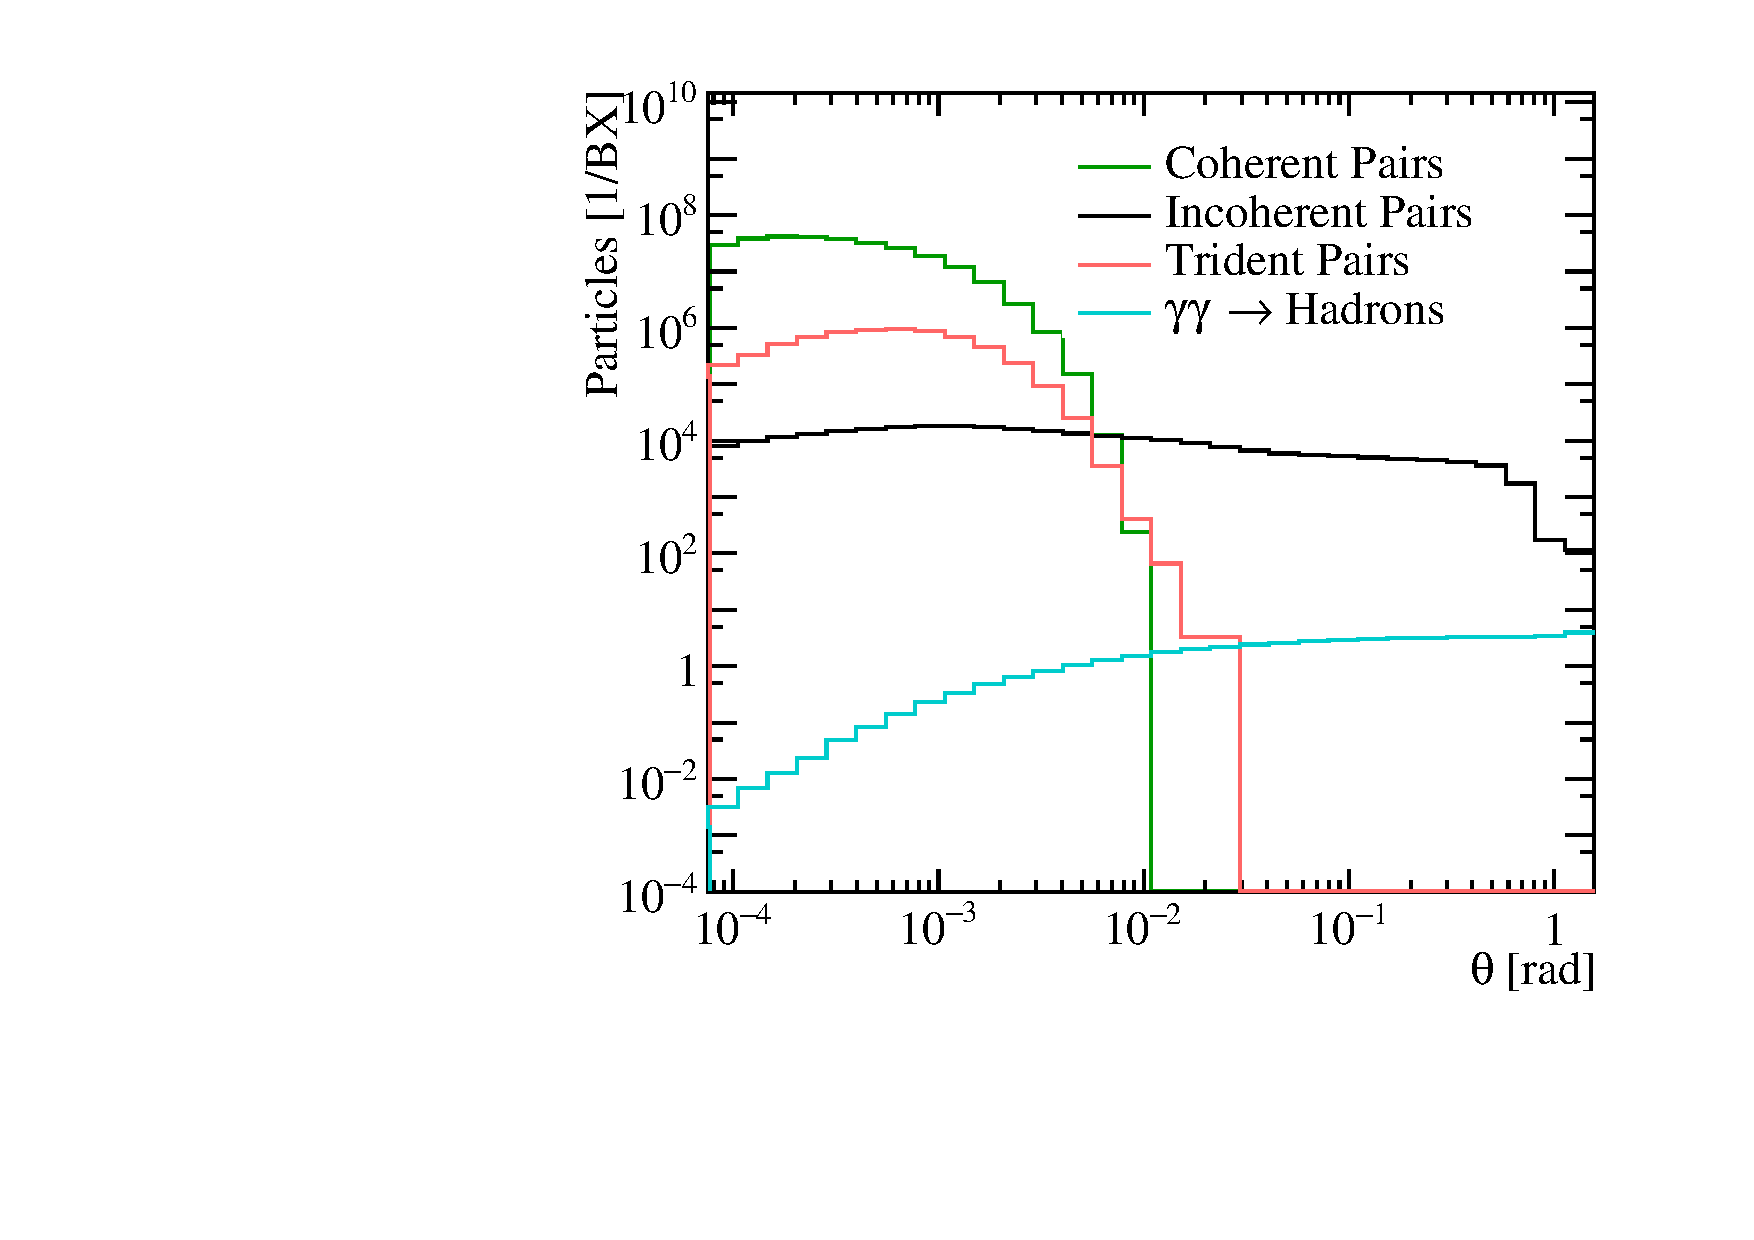
\includegraphics[width=0.5\textwidth]{FutureLinearColliders/Plots/CDRPlots/BackgroundAngleCut.pdf}
\caption[]{Angular distribution of number of particles for beam induced backgrounds for CLIC at $\sqrt{s} = 3$ TeV.  Taken from CLIC CDR.}
\label{fig:backgroundangle}
\end{figure}
  %% Theory - Higgs and EFT 
% \chapter{Theory}
\label{chap:theory}

\chapterquote{There, sir! that is the perfection of vessels!}
{Jules Verne, 1828--1905}

\section{Calorimetry}
% Probably start taking about EM showers and then move onto differences later.
% Particle Showers

\subsection{Electromagnetic Showers}
% Explain what happens when an electron passes through matter
When an electron passes through a material there are several ways different eenrgy loss mechanisms such as ionisation, nuclear excitation, nucelar inrerations, bremsstrahlung and \delta ray production (high energy electron knoack on).  These all have energy dependancies and vary from material to material, however, at the highest energies, such as those found in modern day particle collider experiments, the dominant energy loss meachnism is bremsstrahlung.  Bremsstrahlung is the process by which a photon is radiated off a charged particle as it interacts with the electromagnetic field of a nucleus.  The energy spectrum of the photons is continuous with values ranging up to the energy of the incoming electron (passage of particles through matter).  The peak of the photon energy spectrum from bremsstrahlung occurs at low values of the fractional energy lossed from the incoming particle, as shown in figure BLAH (p20 pptm, 32.12) indicating that in general several photons will be produced from a decelerating charged particle.  

% Explain what happens when a photon passes through matter
The incoming electron energy is thus distributed into serveal bremsstrahlung photons, which in turn deposit energy within the absorbing material through different mechanisms such as the photoelectric effect, Compton scattering and pair-production.  Again, at high energies a single process is dominant, which in this case is pair production whereby an $\text{e}^{+}\text{e}^{-}$ pair are produced from the interaction of a photon in the field of a charged particle, which in this case would be from the nucleus or the electrons of the absorber material atoms (p22 pptm, 32.15).  The $\text{e}^{+}$ will then go onto annihilate with an the $\text{e}^{-}$ in the absorber material producing two photons (spin conservation) and, if the energies are sufficiecntly high, the $\text{e}^{-}$ from the pair production will produce further bremsstrahlung photons.  

% Explain how both combine to make EM shower
The combination of these two mechanims mean that when an electron enters a material a shower of particles are produced from a chain reaction bremsstrahlung and pair production mechanisms.  This is known as an electromagentic shower.  The same shower mechanics also apply if the incoming particle were a positron, annihilation occuring first, or a photon, pair-production occuring first.  

\subsection{Detection of Electromagnetic Showers}
The goal of effective calorimetry is to get an accurate estimate of the energy of the incoming particle based on the measurements that can be made from the showering particles.  A commen technique for this would be to count the number of ionisation tracks produced in the electromagnetic shower.  The number of tracks will be directly proportional to the energy of the incoming particle as the higher the energy of the incoming particle the larger the number of showering particles and so the larger the number of tracks appearing in the shower.  




Calorimetry relies upon the assumption that the energy deposited within a detector is directly proprtional to the energy of the incoming particle.  The incoming particle if charged will deposit energy throughout the calorimeter via ionisation.  However, the incoming particle may also begin a particle shower.  This occurs when the incoming particle interacts via some process with the material inside the calorimeter and produces a cascase of secondard particles.  These secondary particles may then go on to shower later in the calorimeter.  Each particle in this heirarchy will deposit energy within the detector in various ways such as ionisation, exciting of atomic nuclei, collision with nuclei etc.  These energy deposits if recorded can then be summed to give a measurement of the initial particles energy.

% Why Gaussian
Effective calorimetry then becomes a counting exercise to measure as many of these energy deposits as well as possible.  These energy deposits can be recorded in multiple ways depending upon the choice of detector concept, however, these methods exclusively involve counting either the number of charged tracks, e.g. silicon detectors, or the number of photons, e.g. PMT detector, within the particle shower.

For example consider a silicon detector.  If we denote the sum of all the ionisation track lengths of a particle shower within this detector as $T_{0}$ then this is propartional to the number of ionising particles in the shower $N$.  In this case $N = E_{0}/\epsilon$ where $E_{0}$ is the energy of the particle initiating the shower and $\epsilon$ is the average particle energy within the shower.  This means the energy measurement $E_{0}$ is directly prortional to the number of ionised tracks in the shower.  So if $E \propto N$ then $\sigma_{E} \propto \sigma_{N} = \sqrt{N}$.  The last statement holds true as Poissonian statistics hold for measuring the signal $N$.  In the limit of large $N$, which is the typical case for a calorimeter the Poissonian statistics behave as Gaussian statistics and calorimetry yeilds Gaussian distributions for reconstructed energy measurements.  Therefore, the resolution in an ideal calorimeter goes as $\frac{\sigma_{E}}{E} \propto \frac{1}{\sqrt{E}}$.  The same arguement can be applied when we consider counting the number of photons instead of ionisation tracks in the shower.

% Resolution Terms
There are, however, other sources contributing to the resolution of a calorimeter that must be considered.  In general calorimeter energy resolutions are quotes using the following form:

\begin{equation}
\frac{\sigma_{E}}{E} = \frac{a}{\sqrt{E}} \oplus \frac{b}{E} \oplus c
\end{equation}

There are many different contributing sources to the resolution, these include:
\begin{enumerate}
\item Stoichastic term:  This term contributes to the resolution due to the statistical nature of counting quanta to get a measurement.
\item Noise term:  A noise term can also be added to the resolution that scales as $\frac{1}{E}$.  This is the case as the effect of noise on $\sigma_{E}$ is independant of energy, therefore$\sigma_{E}{E} \propto \frac{1}{E}$.
\item Constant term:  Accounts for effects such as leakage that grow with energy.  If $\sigma_{E} \propto E$ then a constant term is added to the resolution.
\end{enumerate}

% Sampling
In a sampling calorimetry the energy is deposited in the active layers of the calorimeter and this information is used to infer the energy deposited in the adjacent absorber layers.







\section{Particle Flow Calorimetry}
\label{sec:unitarisation}

\subsection{Overview}

Particle flow calorimetry is a method of calorimetry where the goal is to reconstruct every visible particle in any given event.  This prcoesses has numerous advantages over traditional calorimetry in that it yeilds superior energy resolutions as well as more topological information that can be used further downstream in physics analyses.  Careful use of this approach to calorimetry allows us to make signficant strides forward in physics understanding in comparison to traditional calorimetric methods.

The application of particle flow calorimetry creates new challenges for detector response on both the hardware and software side.  Fine granularity calorimeters are crucial to be able to track the energy deposits from individual particles and sophisticated pattern recongition software is essential for piecing these energy deposits back together into reconstructed particles.  For particle flow calorimetry to be successful there has to be a synergy between the hardware and software so that the two work together well with success being dictated by physics performance.  

The immense benefits offered by particle flow calorimetry have made it the front runner in terms of the calorimetric approach and as such has been adopted by the future linear lepton-lepton collider.  

\subsection{Paradigm}

The principle of particle flow calorimetry is a simple one, that is to record the energy deposited by a particle in a dectector in the subsystem that offers the best energy resolution.  While a relatively simple aim the application of such a paradigm is challenging as different particles deposit energy throughout the detector in different regions.  

The stable particles that it is possible to measure in a particle collider detector are relatively few in number and can be broken into three categories depending upon their energy depositions.  There are:

\begin{itemize}
\item Charged hardons.  These produce energy depoits in the tracker and both the electromangetic and hadronics calorimeters.
\item Neutral hadrons.  These produce energy depoits in the electromangetic and hadronics calorimeters.
\item Photons.  These produce energy deposits primarily in the electromangetic calorimeters. 
\end{itemize}

As the energy resolution offered by the tracker is signifcantly better that that offered by the calorimeters it is desirable to measure the energy of charged particles in the tracker.  As photons and neutral hadrons do not produce tracks these energy deposits must come from the calorimeter.  This approach is to be contrasted with traditional calorimetry where all energy deposits arise from the calorimeters.  


\section{Physics Theory }

% \chapter{Anomalous Gauge Coupling Theory}
\label{chap:anomalousgaugecouplingtheory}

\chapterquote{"Meaningless! Meaningless!" says the Teacher.  "Utterly meaningless! Everything is meaningless."}
{Ecclesiastes 1:2}

Presented in chapter \ref{chap:PhysicsAnalysis} is an analysis of the sensitivity of the CLIC experiment to the anomalous gauge couplings $\alpha_{4}$ and $\alpha_{5}$ through the vector boson scattering process.  Here, a brief description of the Standard Model of particle physics and a deeper discussion of the anomalous coupling theory studied in chapter \ref{chap:PhysicsAnalysis} is given.  

%========================================================================================
%========================================================================================
%
\section{The Standard Model}
The Standard Model is a non-abelian gauge theory of the $\text{SU}(3) \times \text{SU}(2)_{\text{L}} \times \text{U}(1)$ symmetry group.  It provides a description of three of the four fundamental forces of nature: the electromagnetic, weak and strong nuclear forces \cite{Griffiths:1987tj,Peskin:1995ev}.  The Standard Model contains a total of 24 fermion fields: six flavours of quark each with three colours and six leptons.  A summary of the properties of these particles is given in table \ref{table:smleptons} and \ref{table:smquarks}.  As these fields, $\psi$, are spin-$\frac{1}{2}$, they obey the Dirac equation
%
\begin{equation}
\mathcal{L} = \overline{\psi}(i \slashed{\partial} - m)\psi \text{ ,}
\end{equation}
%
\noindent where $\mathcal{L}$ is the Lagrangian density and $m$ is a mass term.  The derivative term, $\slashed{\partial} = \gamma^{\mu}\partial_{\mu}$, represents a summation over the partial \textcolor{blue}{derivative}, $\partial^{\mu} = (\frac{\partial}{\partial{t}},\frac{\partial}{\partial{x}},\frac{\partial}{\partial{y}},\frac{\partial}{\partial{z}})$, of the field $\psi$ and the gamma matrices, $\gamma^{\mu}$.  Each of the gauge transformations of the Standard Model are defined by a unitary operator \textrm{U}, which acts to transform the vector space, $\Psi$, formed from a combination of fermion fields, $\psi$, in the following way
%
\begin{equation}
\Psi \rightarrow \Psi' = \textrm{U}\Psi \text{ .}
\end{equation}
%
\begin{table}[h!]
\centering
\begin{tabular}{l l r r r}
\hline
Generation & Particle & Mass [MeV] & Spin & \textcolor{blue}{\textit{Q}}/\textit{e} \\
\hline
1 & $e^{-}$ & $0.548579909070\pm0.000000000016$ & 1/2 & $-1$ \\
& $\nu_{e}$ & - & 1/2 & 0 \\
\hline
2 & $\mu^{-}$ & $105.6583745\pm0.0000024$ & 1/2 & $-1$ \\
& $\nu_{\mu}$ & - & 1/2 & 0 \\
\hline
3 & $\tau^{-}$ & $1776.86\pm0.12$ & 1/2 & $-1$ \\
& $\nu_{\tau}$ & - & 1/2 & 0 \\
\end{tabular}
\caption[The mass, spin and electric charge (\textcolor{blue}{\textit{Q}}) of the leptons found in the Standard Model \cite{Beringer:1900zz}.  Neutrino masses have not been included in the above table as precise measurements are yet to be made.  However, oscillations between different neutrino flavour states have been observed, which indicates that the flavour and mass eigenstates differ and that the neutrinos have a non-zero mass.  The current upper bound on neutrino mass measurements is 2 eV.]{The mass, spin and electric charge (\textcolor{blue}{\textit{Q}}) of the leptons found in the Standard Model \cite{Beringer:1900zz}.  Neutrino masses have not been included in the above table as precise measurements are yet to be made.  However, oscillations between different neutrino flavour states have been observed, which indicates that the flavour and mass eigenstates differ and that the neutrinos have a non-zero mass.  The current upper bound on neutrino mass measurements is 2 eV.}
\label{table:smleptons}
\end{table}
%
\begin{table}[h!]
\centering
\begin{tabular}{l l r r r}
\hline
Generation & Particle & Mass [MeV] & Spin & \textcolor{blue}{\textit{Q}}/\textit{e} \\
\hline
1 & $u$ & $2.2^{+0.6}_{-0.4}$ & 1/2 & $+2$/3 \\
 & $d$ & $4.7^{+0.5}_{-0.4}$ & 1/2 & $-1$/3 \\
\hline
2 & $c$ & $1270\pm30$ & 1/2 & $+2$/3 \\
 & $s$ & $98^{+8}_{-4}$ & 1/2 & $+2$/3 \\
\hline
3 & $t$ & $173210 \pm 510 \pm 710$ & 1/2 & $+2$/3 \\
 & $b$ & $4180^{+40}_{-30}$ & 1/2 & $-1$/3 \\
\end{tabular}
\caption[The mass, spin and electric charge (\textcolor{blue}{\textit{Q}}) of the quarks found in the Standard Model \cite{Beringer:1900zz}.  Each of the particles in the above table corresponds to three fermion fields, one for each of the three colours of the SU(3) symmetry.]{The mass, spin and electric charge (\textcolor{blue}{\textit{Q}}) of the quarks found in the Standard Model \cite{Beringer:1900zz}.  Each of the particles in the above table corresponds to three fermion fields, one for each of the three colours of the SU(3) symmetry.} 
\label{table:smquarks}
\end{table}

In the Standard Model, the Lagrangian density describing the fermion fields is invariant under a $\text{SU}(3)$, $\text{SU}(2)_{\text{L}}$ and U(1) gauge transformations.  The $\text{SU}(2)_{L}$ gauge symmetry acts on doublets formed of pairs of left handed chiral components of the fermion fields, $\psi_{L} = \frac{1}{2}(1-\gamma_{5})\psi$, while the right handed components, $\psi_{R} = \frac{1}{2}(1+\gamma_{5})\psi$, transform trivially as singlets \cite{Weinberg:1967tq}.  Similarly, the SU(3) symmetry acts on triplets formed of the fermion fields for each flavour of quark.  All fields transform under the fundamental representation of U(1).  The invariance of the Standard Model Lagrangian to these gauge transformations is established by introducing 12 gauge fields, summarised in table \ref{table:smbosons}, through the covariant \textcolor{blue}{derivative} of the fermion fields
%
\begin{equation}
\partial^{\mu} \rightarrow D^{\mu} = \partial^{\mu} + ig_{1}YB^{\mu} + ig_{2} \textbf{T} \cdot \textbf{W}^{\mu} + ig_{3}\textbf{X} \cdot \textbf{G}^{\mu} \text{ ,}
\end{equation}
%
\noindent where $B^{\mu}$ is the gauge field for the U(1) symmetry, $\textbf{W}^{\mu}$ ($\text{W}^{\mu}_{j}, j =1,2,3$) are the fields of the $\text{SU}(2)_{\text{L}}$ symmetry and $\textbf{G}^{\mu}$ ($\text{G}^{\mu}_{j}, j =1,..,8$) are the fields of the SU(3).  $Y$ is the weak hypercharge, which relates to the chirality and flavour of the fermion field that it is associated to.  The three coefficients $g_{1}$, $g_{2}$ and $g_{3}$ are coupling constants related to the three gauged symmetry groups in the Standard Model.  Mixing of the gauge fields for the U(1) and SU(2) symmetry of the form
%
\begin{equation}
\text{Z}_{\mu} = \text{cos}{\theta_{W}} \text{W}^{3}_{\mu} - \text{sin}{\theta_{W}} \text{B}_{\mu} \text{ ,}\\
\text{A}_{\mu} = \text{sin}{\theta_{W}} \text{W}^{3}_{\mu} + \text{cos}{\theta_{W}} \text{B}_{\mu} \text{ ,}\\
\text{W}^{\pm}_{\mu} = \frac{1}{\sqrt{2}}(\text{W}^{1}_{\mu} \mp i \text{W}^{2}_{\mu}) \text{ ,}
\end{equation}
%
\noindent where
%
\begin{equation}
\text{cos}{\theta_{W}} = \frac{g_{2}}{g_{1}+g_{2}} \text{ and } \text{sin}{\theta_{W}} = \frac{g_{1}}{g_{1}+g_{2}} \text{ ,}
\end{equation}
%
\noindent gives the electroweak gauge bosons; $\text{W}^{\pm}$, Z and $\gamma$.  This mixing ensures that the $\text{W}^{\pm}$ and Z bosons become massive, while the $\gamma$ remains massless.  The $\text{G}^{\mu}_{j}$ fields are the eight massless gluons of the strong force.   $\textbf{T}$ and $\textbf{X}$ are the generators for the SU(2) and SU(3) symmetries, which are typically chosen as
%
\begin{equation}
T_{i} = \frac{1}{2}\tau_{i} \text{ ,} \\
X_{i} = \frac{1}{2}\lambda_{i} \text{ ,} \\
\end{equation}
%
\noindent where $\tau$ and $\lambda$ are the Pauli and the Gell-Mann matrices\textcolor{blue}{,} respectively.  
%
\begin{table}[h!]
\centering
\begin{tabular}{l l r r r}
\hline
Force & Particle & Mass [GeV] & Spin & \textcolor{blue}{\textit{Q}}/\textit{e} \\
\hline
Electromagnetic & $\gamma$ & 0 & 1 & 0 \\
\hline
Weak Nuclear & $\text{W}^{\pm}$ & $80.385 \pm 0.015$ & 1 & $\pm1$ \\
& Z & $91.1876 \pm 0.0021$ & 1 & 0 \\
\hline
Strong Nuclear & $g$ ($\times 8$ colours) & 0 & 1 & 0 \\
\hline
Higgs & H & $125.1 \pm 0.3$ & 0 & 0 \\
\end{tabular}
\caption[The mass, spin and electric charge (\textcolor{blue}{\textit{Q}}) of the gauge bosons found in the Standard Model \cite{Beringer:1900zz}.  The $\gamma$ and $g$s theoretically have zero mass, which is consistent with measurements.  The upper bound on the $\gamma$ mass has been measured at $10^{-18}$ eV, while gluon masses of up to a few MeV have not been precluded.  The upper bound on the magnitude of the charge of the $\gamma$ is measured at $10^{-35}$.]{The mass, spin and electric charge (\textcolor{blue}{\textit{Q}}) of the gauge bosons found in the Standard Model \cite{Beringer:1900zz}.  The $\gamma$ and $g$s theoretically have zero mass, which is consistent with measurements.  The upper bound on the $\gamma$ mass has been measured at $10^{-18}$ eV, while gluon masses of up to a few MeV have not been precluded.  The upper bound on the magnitude of the charge of the $\gamma$ is measured at $10^{-35}$.}
\label{table:smbosons}
\end{table}
%
The gauge fields of the Standard Model, $B_{\mu}$, $\textbf{W}_{\mu}$ and $\textbf{G}_{\mu}$, transform under the gauge transformations as
%
\begin{equation}
K_{\mu} \rightarrow K'_{\mu} = UK_{\mu}U^{\dagger} + \frac{i}{g}(\partial^{\mu}U)U^{\dagger} \text{ ,} 
\end{equation}
%
\noindent where $K_{\mu}$ is any of $B_{\mu}$, $\textbf{W}_{\mu}$ and $\textbf{G}_{\mu}$ and $g$ is the coupling constant associated to the relevant gauged symmetry group.  As the $B_{\mu}$, $\textbf{W}_{\mu}$ and $\textbf{G}_{\mu}$ gauge fields are spin-1, they are described by the Proca Lagrangian density
%
\begin{equation}
\mathcal{L} = -\frac{1}{4}F^{{\mu}{\nu}}_{i}F_{{\mu}{\nu}{i}} + \frac{1}{2}m_{K}^{2}K_{i\mu}K^{\mu}_{i} \text{ ,} 
\end{equation}
%
\noindent where
%
\begin{equation}
F^{{\mu}{\nu}}_{i} = \partial^{\mu}K^{\nu}_{i} - \partial^{\nu}K^{\mu}_{i} - gf_{ijk}K^{\mu}_{j}K^{\nu}_{k} \text{ ,} 
\end{equation}
%
\noindent \textcolor{blue}{and} $f_{ijk}$ are the fully anti-symmetric structure constants of the group, $K^{\mu}_{i}$ is the $i^{th}$ gauge field of the group and $m_{K}$ is a mass term for the gauge boson.  The structure constants are defined from the commutation relations between generators of the symmetry group
%
\begin{equation}
[T_{i},T_{j}] = if_{ijk}T_{k} \text{.} 
\end{equation}
%
\noindent These structure constants govern the self-interactions for the gauge bosons.  There is only one structure constant for the U(1) symmetry, which is zero, as the U(1) symmetry is abelian.  The SU(2) symmetry structure constants are $f_{ijk} = \epsilon_{ijk}$, where $\epsilon_{ijk}$ is the Levi-Civita tensor.  Due to the symmetries that are present in the Standard Model, $m_{K} = 0$ for all the gauge fields, however, it is clear that this is not the case.  

%========================================================================================
%========================================================================================

\section{Higgs Physics}
\label{sec:higgsphysics}
Mass terms are generated in the Standard Model by introducing a Higgs field that undergoes spontaneous symmetry breaking.  This allows the gauge bosons, as well as the quarks and leptons, to obtain a mass, while still respecting the gauge symmetries found in the Standard Model.  

%========================================================================================

\subsection{Spontaneous Symmetry Breaking}
\label{sec:ssb}
To illustrate spontaneous symmetry breaking, consider a complex scalar field \psi with the Klein-Gordon Lagrangian
%
\begin{equation}
\mathcal{L} = \partial^{\mu} \psi^{*} \partial_{\mu} \psi -m^{2} |\psi|^{2} = \partial^{\mu} \psi^{*} \partial_{\mu} \psi - V(\psi) \text{ ,}
\label{equ:kleingordon}
\end{equation}
%
\noindent where $m$ is a mass term and $V(\psi)$ is the potential \textcolor{blue}{of} the field $\psi$.  This Lagrangian density is invariant under the global symmetry $\psi \rightarrow e^{i\alpha} \psi$.  By adding extra terms to the Lagrangian, which retain the invariance to this global symmetry, it is possible to modify the interactions of this scalar field.  Consider modifying the potential of the scalar field to the following
%
\begin{equation}
\text{V}(\psi) = m^{2}|\psi|^{2} + \lambda |\psi|^{4} \text{ .}
\end{equation}
%
\noindent If $m^{2} > 0$, the potential has a \textcolor{blue}{minimum} at zero, however, if $m^{2} < 0$ then the minima exists on a circle in the complex $\psi$ plane, which is centred at $(0,0)$ and has radius $v = \sqrt{-m^{2}/\lambda}$.  To quantise this theory it is necessary to expand about the \textcolor{blue}{minimum} of the potential.  However, in the case of $m^{2} < 0$ there are an infinite number of choices of minima to expand about.  Irrespective of the choice of \textcolor{blue}{minimum} used to expand the field about, the symmetry $\psi \rightarrow e^{i\alpha} \psi$ is broken.  Fluctuations about the \textcolor{blue}{minimum} along the degenerate direction leave the potential unchanged, which is a consequence of the breaking of the $\psi \rightarrow e^{i\alpha} \psi$ symmetry; this is known as spontaneous symmetry breaking.  Goldstone's theorem \cite{Goldstone:1962es} implies that, for Lorentz-invariant theories, spontaneous symmetry breaking always leads to the existence of massless particles known as Goldstone bosons.  If the complex scalar field $\psi$ is expanded about the non-zero minima, $\psi$ takes the form
%
\begin{equation}
\psi = \frac{1}{\sqrt{2}}(v + \psi_{1} + i \psi_{2}) \text{ ,}
\label{equ:minima}
\end{equation}
%
\noindent where $\psi_{1}$ and $\psi_{2}$ are real fields and $v = \sqrt{-m^{2}/\lambda}$.  Applying this parameterisation to the Lagrangian yields a mass term of $\sqrt{-m^{2}}$ for the $\psi_{1}$ field.  However, there is no corresponding mass term for the $\psi_{2}$ field, which indicates that it is massless as predicated by Goldstone's theorem
%
\begin{equation}
\mathcal{L} = \frac{1}{2}\partial^{\mu} \psi_{1} \partial_{\mu} \psi_{1} + \frac{1}{2}\partial^{\mu} \psi_{2} \partial_{\mu} \psi_{2} - m^{2}|\psi_{1}|^{2} + ... \text{ \textcolor{blue}{.}}
\end{equation}

Spontaneous symmetry breaking is the origin of gauge boson mass terms when applied to local symmetries instead of global ones.  For example, consider the global symmetry, $\psi \rightarrow e^{i\alpha} \psi$ that exists in equation \ref{equ:kleingordon}.  If this global symmetry is promoted to a local symmetry by letting $\alpha \rightarrow \alpha(x)$ and $\partial^{\mu} \rightarrow D^{\mu} = \partial^{\mu} + iA^{\mu}$, where $A^{\mu}$ \textcolor{blue}{is} the gauge field that transforms as $A^{\mu} \rightarrow A^{\mu} - \partial^{\mu}\alpha(x)$, the Lagrangian becomes
%
\begin{equation}
\mathcal{L} = (D^{\mu} \psi)^{*} (D_{\mu} \psi) - m^{2} |\psi|^{2} - \lambda |\psi|^{4} \text{ .}
\end{equation}
%
\noindent If the $\psi$ field is expanded about a non-zero \textcolor{blue}{minimum} in the potential, i.e. $m^{2} < 0$ and $v = \sqrt{-m^{2}/\lambda}$, as was done in equation \ref{equ:minima}, then a gauge boson mass term, $+\frac{v^{2}}{2} A^{\mu} A_{\mu}$, is generated from the $(D^{\mu} \psi)^{*} (D_{\mu} \psi)$ term.

%========================================================================================

\subsection{Electroweak Interactions}
\label{sec:ewint}
The electroweak sector of the Standard Model is that related to the $\text{SU}(2)_{\text{L}} \times \text{U}(1)$ symmetry \cite{Ellis:2013jnq}.  In this sector, spontaneous symmetry breaking must occur in such a way as to give three massive gauge bosons,  $\text{W}^{\pm}$ and Z, and one massless gauge boson, the $\gamma$.  This can be achieved through a Higgs field, H, that transforms as a doublet under the $\text{SU}(2)_{\text{L}}$ symmetry.  The Lagrangian for this field is
%
\begin{equation}
\mathcal{L}_{Higgs} = (D_{\mu}\text{H})^{\dagger}D^{\mu}\text{H} - \text{V}(\text{H}) \text{ .}
\end{equation}
%
\noindent The Higgs potential, V(H), is
%
\begin{equation}
\text{V}(\text{H}) = -\mu^{2}\text{H}^{\dagger}\text{H} + \lambda (\text{H}^{\dagger}\text{H})^{2} \text{ ,}
\end{equation}
%
\noindent where $\mu$ and $\lambda$ are constants.  The covariant derivative of this Higgs field must satisfy the $\text{SU}(2)_{\text{L}} \times \text{U}(1)$ gauge symmetry meaning it takes the form
%
\begin{equation}
D_{\mu} \text{H} = (\partial_{\mu} + ig_{1}YB_{\mu} + ig_{2}\frac{\tau^{i}}{2}W^{i}_{\mu})\text{H} \text{ ,}
\end{equation}
%
\noindent where $g_{1}$ and $g_{2}$ are coupling constants for the U(1) and $\text{SU}(2)_{\text{L}}$ gauged symmetries\textcolor{blue}{,} respectively, $Y = \frac{1}{2}$ is the weak hypercharge of the Higgs and $\tau^{i}$ are the Pauli matrices.  $B_{\mu}$ and $W^{i}_{\mu}$ are the gauge fields for the U(1) and $\text{SU}(2)_{\text{L}}$ gauged symmetries respectively.  

Consider spontaneously breaking the symmetry in the Higgs sector by expanding the Higgs field about a non-zero vacuum expectation value (vev)
%
\begin{equation}
\langle \text{H} \rangle = \binom{0}{\frac{v}{\sqrt{2}}} \text{ ,}
\label{equ:higgsmin}
\end{equation}
%
\noindent where the minima of the field is defined as
%
\begin{equation}
\frac{v}{\sqrt{2}} = \sqrt{\frac{\mu^{2}}{2\lambda}} \text{ ,}
\end{equation}
%
\noindent where $v$ real.  In that case, the kinematic term in the Higgs Lagrangian, $D^{\mu} \text{H}^{\dagger} D_{\mu} \text{H}$, contains mass terms for the gauge bosons
%
\begin{equation}
D^{\mu} \text{H}^{\dagger} D_{\mu} \text{H} \subset \frac{v^{2}}{2}(ig_{1}YB^{\mu} + ig_{2}\frac{\tau^{i}}{2}W^{i\mu})(ig_{1}YB_{\mu} + ig_{2}\frac{\tau^{i}}{2}W^{i}_{\mu}) \text{ .}
\end{equation}
%
\noindent If there is mixing of the $\text{SU}(2)_{\text{L}}$ and U(1) fields of the form
%
\begin{equation}
\text{Z}_{\mu} = \text{cos}{\theta_{W}} \text{W}^{3}_{\mu} - \text{sin}{\theta_{W}} \text{B}_{\mu} \text{ ,}\\
\text{A}_{\mu} = \text{sin}{\theta_{W}} \text{W}^{3}_{\mu} + \text{cos}{\theta_{W}} \text{B}_{\mu} \text{ ,}\\
\text{W}^{\pm}_{\mu} = \frac{1}{\sqrt{2}}(\text{W}^{1}_{\mu} \mp i \text{W}^{2}_{\mu}) \text{ ,}
\end{equation}
%
\noindent then the following gauge boson mass terms are generated
%
\begin{equation}
\frac{(gv)^{2}}{4} \text{W}^{+}_{\mu} \text{W}^{-\mu} + \frac{(g^{2} + g'^{2})v^{2}}{8} \text{Z}_{\mu} \text{Z}^{\mu} \text{ .}
\end{equation}
%
\noindent The gauge boson masses generated by spontaneous symmetry breaking of the Higgs field are
%
\begin{equation}
\begin{aligned}
m_{\text{W}} = & \frac{gv}{2} \text{ ,} \\
m_{\text{Z}} = & \frac{v\sqrt{g^{2} + g'^{2}}}{2} = \frac{m_{W}}{\text{cos}{\theta_{W}}} \text{ ,} \\
m_{\text{A}} = & 0 \text{ ,}
\end{aligned}
\end{equation}
%
\noindent where $\theta_{W}$ is the Weinberg angle.  This mixing produces a massless gauge boson, the $\gamma$, and three massive gauge bosons, the $W^{\pm}$ and $Z$.  By acquiring a non-zero vev, the Higgs field breaks the $\text{SU}(2)_{\text{L}} \times \text{U}(1)$ symmetry that was present in the Lagrangian to the $\text{U}(1)_{em}$ symmetry of electromagnetism.  

The ratio of the masses of the $W^{\pm}$ and $Z$ bosons is predicted when spontaneous symmetry breaking occurs in the Higgs sector.  This prediction sets the $\rho$ parameter to unity, where the $\rho$ parameter is defined as
%
\begin{equation}
\rho = \frac{m_{\text{W}}^{2}}{m_{\text{Z}}^{2}\text{cos}{\theta_{W}}^{2}} = 1\text{ .}
\label{equ:custodialsymmetry}
\end{equation}
%
\noindent This is a consequence of the Higgs potential containing custodial symmetry \cite{Beringer:1900zz}.  As the $\rho$ parameter has been experimentally measured to be $1.00040 \pm 0.00024$ \cite{Agashe:2014kda}, it is clear that any extension to the Standard Model should retain this result.

%========================================================================================

\subsubsection{Custodial Symmetry}
The Standard Model Higgs field is defined by the Lagrangian
%
\begin{equation}
\mathcal{L}_{Higgs} = (D_{\mu}\text{H})^{\dagger}D^{\mu}\text{H} - \text{V}(\text{H}) \text{,}
\end{equation}
%
\noindent where
%
\begin{equation}
\text{V}(\text{H}) = -\mu^{2}\text{H}^{\dagger}\text{H} + \lambda (\text{H}^{\dagger}\text{H})^{2} \text{ ,}
\end{equation}
%
\noindent and $\mu$ and $\lambda$ are constants.  By construction the Higgs sector of the Standard Model is invariant under local $\text{SU}(2)_{\text{L}} \times \text{U}(1)$ gauge transformations.  However, a larger global symmetry also exists in this sector, which can be seen by examining the Higgs doublet \cite{Ellis:1991qj}
%
\begin{equation}
\text{H} = \binom{\psi^{+}}{\psi^{0}} = \binom{\psi_{1} + i\psi_{2}}{\psi_{3} + i\psi_{4}} \text{ .}
\end{equation}
%
\noindent All the terms in the Higgs potential involve $\text{H}^{\dagger}\text{H} = \psi_{1}^{2} + \psi_{2}^{2} + \psi_{3}^{2} + \psi_{4}^{2}$, which is invariant under any rotation of these four components and hence under \textcolor{blue}{an} SO(4) global symmetry.  In general, $\text{SO}(4) \cong \text{SU}(2) \times \text{SU}(2)$, where $\cong$ denotes an isomorphism.  In the case of the Higgs sector $\text{SO}(4) \cong \text{SU}(2)_{L} \times \text{SU}(2)_{R}$ where the $\text{SU}(2)_{L}$ symmetry is the gauged symmetry of the Standard Model.  This symmetry can be manifested using an alternative parameterisation \cite{Andersen:2011yj} of the Higgs field
%
\begin{equation}
\Phi = (i\tau_{2}\text{H}, \text{H}) = 
\begin{pmatrix}
\psi^{0*} & \psi^{+} \\
-\psi^{+*} & \psi^{0}
\end{pmatrix} 
\text{ .}
\end{equation}
%
\noindent In this parametrisation the Higgs Lagrangian, $\mathcal{L}_{Higgs}$, becomes
%
\begin{equation}
\mathcal{L}_{Higgs} =  \frac{1}{2}\text{Tr}[(D_{\mu}\Phi)^{\dagger}D^{\mu}\Phi] + \mu^{2}\text{Tr}[\Phi^{\dagger}\Phi] - \lambda \text{Tr}[\Phi^{\dagger}\Phi\Phi^{\dagger}\Phi] \text{ ,}
\end{equation}
%
\noindent which is invariant under transformations of the form
%
\begin{equation}
\Phi \rightarrow U_{L} \Phi U_{R}^{\dagger} \text{ ,}
\end{equation}
%
\noindent where $U_{L}$ and $U_{R}$ are transformations of the $\text{SU}(2)_{L}$ and $\text{SU}(2)_{R}$ symmetry groups respectively.

When the Higgs field acquires a non-zero vev the $\text{SU}(2)_{L} \times \text{SU}(2)_{R}$ symmetry of the Higgs potential is broken to \textcolor{blue}{an} $\text{SU}(2)_{C}$ symmetry, which is known as custodial symmetry \cite{Grojean:2007zz}.  As $\text{SO}(3) \cong \text{SU}(2)$, symmetry breaking in the Higgs sector is equivalent to \textcolor{blue}{an} SO(4) symmetry being broken to \textcolor{blue}{an} SO(3) symmetry.  This becomes clear when inspecting the form of the Higgs potential after symmetry breaking.  After expanding the Higgs field about the non-zero vev that is defined in equation \ref{equ:higgsmin}, the terms in the Higgs potential involve $\text{H}^{\dagger}\text{H} = (\psi_{3}-v)^{2} + \psi_{1}^{2} + \psi_{2}^{2} + \psi_{4}^{2}$.  Since $\text{H}^{\dagger}\text{H} $ is only invariant to rotations between the $\psi_{1}$, $\psi_{2}$ and $\psi_{4}$ fields, the SO(4) global symmetry of the Higgs potential has been broken by spontaneous symmetry breaking to \textcolor{blue}{an} SO(3) symmetry.

The Higgs field, H, transforms a singlet under this $\text{SU}(2)_{C}$ custodial symmetry, while the $\text{SU}(2)_{L}$ gauge boson fields, $W^{i}_{\mu}$, transform as a triplet.  It is the transformation of the $W^{i}_{\mu}$ fields under the $\text{SU}(2)_{C}$ symmetry that enforces the relationship between the masses of the $W^{\pm}$ and $Z$ gauge bosons and that $\rho$ should equal unity.  It should be noted that the $\text{SU}(2)_{L} \times \text{SU}(2)_{R}$ symmetry only exists in the Higgs sector of the Standard Model.  The $\text{SU}(2)_{R}$ symmetry in the Standard Model is broken by Yukawa couplings of the Higgs to quarks and leptons and by a non-zero coupling to the U(1) gauge symmetry of the Standard Model, $g_{1}$.  However, this breaking of the $\text{SU}(2)_{R}$ symmetry is weak, which means the deviations of $\rho$ from unity are minimal \cite{Grojean:2007zz}.  

%========================================================================================

\section{Effective Field Theory}
\label{sec:eft}
There are a number of features in the observable universe that cannot be accounted for using the Standard Model of particle physics.  However, the Standard Model provides a very good description of the interactions between particles at the energies being probed at modern particle collider experiments.  Any underlying theory governing the interactions of particles must, therefore, behave like the Standard Model over these energies, or distance scales.  Above such energies the theory will deviate from the Standard Model in order to account for the full underlying theory.  Effective field theories (EFTs) work from this premise by assuming that the complete theory has a momentum scale, $\Lambda$, below which Standard Model behaviour is replicated \cite{Degrande:2013rea, Arzt:1993gz}.  

Quantum field theories must be renormalizable to ensure that non-infinite predictions of the coefficients in the Lagrangian can be made and tested \cite{Gripaios:2015qya}.  Infinities arise from non-renormalizable theories due to divergent integrals from loop diagrams that assume the theory being applied is valid at all energy and length scales.  Effective field theories act to avoid such problems by only integrating up to the momentum scale $\Lambda$ and not above it.  At the energy scale being considered, any infinities arising from the loop calculations in the EFT can be absorbed into a finite number of parameters.  This methodology avoids the assumption that the theory in question is applicable to all energy scales and allows measurable predictions to be made.  

As the Standard Model should be replicated at the low energy scale, it is appropriate when creating an EFT Lagrangian to append new operators to the Standard Model Lagrangian to account for areas of new physics.  This gives the general form for an EFT Lagrangian as \cite{Degrande:2013rea}
%
\begin{equation}
\mathcal{L}_{EFT} = \mathcal{L}_{SM} + \sum_{\text{dimension d>4}} \sum_{i} \frac{c_{i}^{(d)}}{\Lambda^{d-4}} \mathcal{O}_{i}^{(d)} \text{ ,}
\label{equ:eft}
\end{equation}
%
\noindent where $\mathcal{L}_{SM}$ is the Standard Model Lagrangian, $c_{i}^{(d)}$ are free parameters, $\mathcal{O}_{i}^{(d)}$ is the $i^{th}$ unique operator with dimension $d$ in the EFT and $\Lambda$ is the EFT momentum scale.  The sum runs over all unique operators with dimension greater than four.  The presence of the $\Lambda^{d-4}$ in the denominator is required to ensure correct dimensionality of the new terms being added to the Lagrangian.  

New physics is introduced by the operators $\mathcal{O}_{i}^{(d)}$, but suppressed by the momentum scale $\Lambda$.  It is assumed that $\Lambda$ is large with respect to the momentum scales that have been examined at pre\textcolor{blue}{-}existing particle collider experiments, therefore, any new physics is suppressed.  Under this assumption, new operators with dimension less than, or equal to, four can be vetoed from the EFT as their effects would be readily observed at preexisting particle collider experiments, due to the $\Lambda^{4-d}$ coefficient.  At energies below the momentum scale, $\Lambda$, it is possible to find the dominant new physics terms in the EFT and consider these as corrections to the Standard Model.  Above this scale the EFT breaks down as operator $\mathcal{O}_{i}^{(d)}$ in $\mathcal{L}_{EFT}$ has a non-negligible coefficient.  In the extremal limit, $\Lambda \rightarrow \infty$, the Standard Model is recovered as new physics is too far out of reach to have any impact on observables.

%========================================================================================

\section{Electroweak Chiral Lagrangian}
The introduction of a Higgs field undergoing spontaneous symmetry breaking is able to produce mass terms in the Lagrangian for the $\text{W}^{\pm}$ and Z bosons.  However, it is possible to introduce these terms by parameterising the Higgs field using the gauge boson fields of the $\text{SU}(2)_{\text{L}}$ Standard Model symmetry \cite{Herrero:1994tj}.  In this approach, the pattern of spontaneous symmetry breaking mirrors that found in the Higgs sector of the Standard Model i.e. a global $\text{SU}(2)_{L} \times \text{SU}(2)_{R}$ symmetry is broken to \textcolor{blue}{an} $\text{SU}(2)_{C}$ symmetry.  This will ensure that the $\rho$ parameter, introduced in section \ref{sec:ewint}, retains a value of unity which is consistent with experimental measurements.  The Standard Model spontaneous symmetry breaking pattern can be replicated using a field, $\Sigma(x)$, which transforms under the $\text{SU}(2)_{L} \times \text{SU}(2)_{R}$ global symmetries as
%
\begin{equation}
\Sigma \rightarrow U_{L} \Sigma U_{R}^{\dagger} \text{ ,}
\end{equation}
%
\noindent where $U_{L}$ and $U_{R}$ are transformations of the $\text{SU}(2)_{L}$ and $\text{SU}(2)_{R}$ symmetry groups\textcolor{blue}{,} respectively\textcolor{blue}{,} and $\Sigma(x)$ is
%
\begin{equation}
\Sigma(x) = \text{exp} \bigg(\frac{-i}{v} \Sigma^{3}_{a=1} \pi^{a}\tau^{a}\bigg)\text{ ,}
\end{equation}
%
\noindent where $\pi^{a}$ are the three would-be Goldstone bosons that exist when the $\text{SU}(2)_{\text{L}} \times \text{U}(1)$ symmetry is broken to $\text{U}(1)_{em}$ \cite{Longhitano:1980tm}.  The $\text{SU}(2)_{\text{L}}$ and $\text{U}(1)$ symmetries of the Standard Model are gauged in the usual way by defining the covariant derivate of the $\Sigma$ field
%
\begin{equation}
\mathcal{D}_{\mu} \Sigma(x) = \partial_{\mu} \Sigma(x) + \frac{ig_{2}}{2}\text{W}_{\mu}^{a}\tau^{a}\Sigma(x) - \frac{ig_{1}}{2}\text{B}_{\mu}\tau^{3}\Sigma(x) \text{ ,}
\end{equation}
%
\noindent where $g_{1}$ and $g_{2}$ are coupling constants for the U(1) and SU$(2)_\text{L}$ symmetries respectively and $\tau^{a}$ are the Pauli spin matrices.  The lowest order derivative term for this $\Sigma$ field that could appear in the Lagrangian is
%
\begin{equation}
\mathcal{L}_{\Sigma} = \frac{v^{2}}{4} \text{Tr} (\mathcal{D}^{\mu} \Sigma^{\dagger} \mathcal{D}_{\mu} \Sigma) = -\frac{v^{2}}{4}\text{Tr}(V_{\mu} V^{\mu}) \text{ ,} 
\end{equation}
%
\noindent where $V_{\mu} = (\mathcal{D}_{\mu}\Sigma) \Sigma^{\dagger}$.  This terms respects all the symmetries present in the Higgs sector of that Standard Model, including the custodial symmetry in the limit $g_{1} \rightarrow 0$.  Furthermore, by expanding this field about a non-zero vev, the $\text{SU}(2)_{L} \times \text{SU}(2)_{R}$ global symmetry is broken to \textcolor{blue}{an} $\text{SU}(2)_{C}$ symmetry exactly as it is in the Standard Model.  For example, if this field is expanded about the point $\Sigma = \textbf{1}$, i.e. the unitary gauge, mass terms for the electroweak gauge bosons are generated that match those produced from spontaneous symmetry breaking of the Higgs field as described in section \ref{sec:ssb}
%
\begin{equation}
\frac{v^{2}}{4}\text{Tr}[V^{\mu}V_{\mu}] = - \frac{(gv)^{2}}{4} \text{W}^{+}_{\mu} \text{W}^{-\mu} - \frac{(g^{2} + g'^{2})v^{2}}{8} \text{Z}_{\mu} \text{Z}^{\mu} \\
\begin{aligned}
m_{\text{A}} = & 0 \text{ ,} \\
m_{\text{W}} = & \frac{gv}{2} \text{ ,} \\
m_{\text{Z}} = & \frac{v\sqrt{g^{2} + g'^{2}}}{2} = \frac{m_{\text{W}}}{\text{cos}{\theta_{W}}} \text{ \textcolor{blue}{.}}
\end{aligned}
\end{equation}

So far, all that has been done is a parameterisation of the Higgs field, however, it was shown by Longhitano \cite{Longhitano:1980tm} that there are several relevant operators involving the $\Sigma$ field that are $\text{SU}(2)_{\text{L}} \times \text{U}(1)$ invariant.  As these operators obey the same symmetries as those found in the Standard Model they should be considered.  This can be done using EFT approach, as discussed in section \ref{sec:eft}.  Of the operators introduced by Longhitano, only two involve quartic massive gauge boson vertices and preserve the custodial symmetry \cite{Belyaev:1998ih}.  These are
%
\begin{equation}
\alpha_{4}\text{Tr}[V^{\mu}V_{\nu}]\text{Tr}[V^{\nu}V_{\mu}] \quad \text{ and } \quad \alpha_{5}\text{Tr}[V^{\mu}V_{\mu}]^{2} \text{ .}
\label{equ:newterms}
\end{equation}
%
\noindent These terms contribute to the massive gauge boson quartic vertices shown in figure \ref{fig:agcvertices}.  The Standard Model already contains triple and quartic vertices involving the electroweak gauge bosons, shown in figure \ref{fig:smtripleandquarticverticestheory}, and these are also present in this EFT approach.  These vertices originate from the kinematic terms in the Proca Lagrangian density $\mathcal{L}_{kin} = -\frac{1}{4}B_{\mu\nu}B^{\mu\nu} - \frac{1}{4}W_{\mu\nu}W^{\mu\nu}$.  Of the vertices showing sensitivity to $\alpha_{4}$ and $\alpha_{5}$, only the vertex shown in figure \ref{fig:agcvertex3} is not present in the Standard Model.  

Both terms shown in equation \ref{equ:newterms} contain dimension 8 operators \cite{Degrande:2013rea} and, with respect to the EFT approach (i.e. equation \ref{equ:eft}) their coefficients are proportional to $\Lambda^{-4}$, where $\Lambda$ is the momentum scale of the new physics being modelled.  In the limit that the momentum scale of new physics is beyond experimental reach, i.e. $\Lambda \rightarrow \infty$, these terms do not contribute to measurable observables and the Standard Model is recovered.  It should be noted that in this case, the Standard Model has been parameterised using the $\Sigma$ field; so, in the limit $\Lambda \rightarrow \infty$, the gauge boson mass terms generated from $\mathcal{L}_{\Sigma}$ do not vanish.  

\begin{figure}[h!]
\subfloat[]{\label{fig:agcvertex1}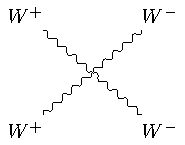
\includegraphics[width=0.3\textwidth]{AnomalousCouplingsTheory/Plots/AGCVertex1.pdf}} 
\subfloat[]{\label{fig:agcvertex2}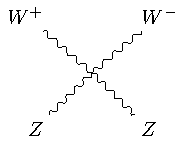
\includegraphics[width=0.3\textwidth]{AnomalousCouplingsTheory/Plots/AGCVertex3.pdf}} 
\subfloat[]{\label{fig:agcvertex3}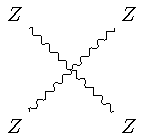
\includegraphics[width=0.2275\textwidth]{AnomalousCouplingsTheory/Plots/AGCVertex2.pdf}} 
\caption[Gauge boson self-coupling vertices that are sensitive to the anomalous gauge couplings $\alpha_{4}$ and $\alpha_{5}$.]{Gauge boson self-coupling vertices that are sensitive to the anomalous gauge couplings $\alpha_{4}$ and $\alpha_{5}$.}
\label{fig:agcvertices}
\end{figure}
% Feynam diagrams of triple and quartic vertices in the standard model.
\begin{figure}[h!]
\subfloat[]{\label{fig:smvertex1}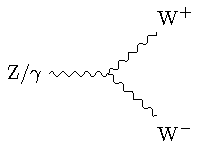
\includegraphics[width=0.3\textwidth]{PhysicsAnalysis/Plots/FeynmanDiagrams/SMVertex1.pdf}} 
\subfloat[]{\label{fig:smvertex2}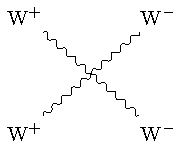
\includegraphics[width=0.3\textwidth]{PhysicsAnalysis/Plots/FeynmanDiagrams/SMVertex2.pdf}} 
\subfloat[]{\label{fig:smvertex3}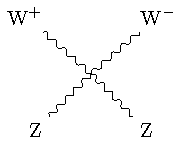
\includegraphics[width=0.3\textwidth]{PhysicsAnalysis/Plots/FeynmanDiagrams/SMVertex3.pdf}} \hfill
\subfloat[]{\label{fig:smvertex4}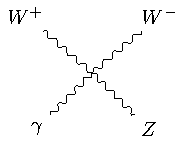
\includegraphics[width=0.3\textwidth]{PhysicsAnalysis/Plots/FeynmanDiagrams/SMVertex4.pdf}} 
\subfloat[]{\label{fig:smvertex5}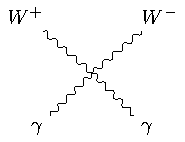
\includegraphics[width=0.3\textwidth]{PhysicsAnalysis/Plots/FeynmanDiagrams/SMVertex5.pdf}} 
\caption[Gauge boson self-coupling vertices in the Standard Model.]{Gauge boson self-coupling vertices in the Standard Model.}
\label{fig:smtripleandquarticverticestheory}
\end{figure}

%========================================================================================

  %% Linear Collider Detectors and Particle Flow
% \chapter{Particle Flow Calorimetry for Future Linear Colliders}
\label{chap:pflowandlcdetectors}

\chapterquote{I am fond of pigs.  Dogs look up to us.  Cats look down on us.  Pigs treat us as equals.}
{Winston Churchill}

%========================================================================================
%========================================================================================

Particle flow calorimetry can provide extremely good jet energy resolutions at a future linear collider.  Jet energy resolution is crucial at the linear collider as many of the interesting processes will be characterised by multi-jet final states.  Many of these multi-jet final states will be produced from the hadronic decays of W and Z bosons and one of the key goals of the future linear collider is to be able to separate these decays.  Separation of these decays can be achieved, however, only by placing a tight requirement on the jet energy resolution; $\sigma_{E}/E \lessapprox 3.5\%$ for 50-500~GeV jets at the ILC and up to 1.5~TeV at CLIC \cite{arXiv:0907.3577}.  The use of particle flow calorimetry will also be highly beneficial for quantifying final states of interest that involving charged leptons and missing momentum.  

%========================================================================================
%========================================================================================

\section{Particle Flow Calorimetry}
The premise of particle flow calorimetry is to use the sub-detector that offers the best energy resolution to measure the energy of any given particle, which corresponds to energy measurements being made in the ECal for $\gamma$s, the HCal for neutral hadrons and, crucially, the tracker for charged particles.  The starkest contrast of this approach to that of traditional calorimetry occurs in the measurement of the energy of charged particles.  In particle flow calorimetry the energy of a charged particle is measured using the curvature of the path it transverses as it bends in a magnetic field, while in traditional calorimetry the energy would be measured using the calorimeters, predominantly the hadronic calorimeter (HCal).  The tracker energy resolution for a single charged particle of energy $E_{X^{\pm}}$ is typically $10^{-4} \times E_{X^{\pm}}^{2}$, while for the HCal it is $\sim 0.55 \times \sqrt{E_{X^{\pm}}}$ \cite{arXiv:0907.3577}.  The energy resolution offered by the tracker is significantly better than that offered by the HCal for energies up to $\sim \mathcal{O}(300 \text{ GeV})$.  This means that particle flow calorimetry has the potential to offer a much better energy resolution for charged particles below $\sim \mathcal{O}(300 \text{ GeV})$, than that of the traditional calorimetry approach.  Particle flow calorimetry offers gains in performance for collision energies well beyond 300 GeV as the average long-lived particle energy for physics processes of interest is typically much less than 300 GeV.  Furthermore, it also leads to a significant improvement in the measurement of jet energies as, after the decay of short-lived particles, approximately 60\% of the energy of a jet is carried in the form of charged particles.  The measurement of jet energies in the particle flow paradigm is summarised in table \ref{table:pflowjet}.  The benefits to the energy resolution, for both charged particles and jets, offered by the particle flow approach to calorimetry is the driving factor behind why it is planned for used at the linear collider experiment.  

\begin{table}[h!]
\centering
\begin{tabular}{ l l l l l}
\hline
Jet  & Detector & Energy & Energy\\
Component &  & Fraction & Resolution\\
\hline
Charged Particles ($X^{\pm}$) & Tracker & $\sim 0.6 E_{j}$ & $10^{-4} \times E_{X^{\pm}}^{2}$ \\
Photons ($\gamma$) & ECal & $\sim 0.3 E_{j}$ & $0.15 \times \sqrt{E_{\gamma}}$ \\
Neutral Hadrons ($X^{0}$) & HCal &$\sim 0.1 E_{j}$ & $0.55 \times \sqrt{E_{X^{0}}}$ \\
\hline
\end{tabular}
\caption[The approximate jet fractions and energy resolutions for charged particles ($X^{\pm}$) of energy $E_{X^{\pm}}$, photons ($\gamma$) of energy $E_{\gamma}$ and neutral hadrons ($X^{0}$) of energy $E_{X^{0}}$.  The energy resolution for photons and neutral hadrons reflects the performance of a linear collider like ECal and HCal respectively.  Taken from \cite{arXiv:0907.3577}.]{The approximate jet fractions and energy resolutions for charged particles ($X^{\pm}$) of energy $E_{X^{\pm}}$, photons ($\gamma$) of energy $E_{\gamma}$ and neutral hadrons ($X^{0}$) of energy $E_{X^{0}}$.  The energy resolution for photons and neutral hadrons reflects the performance of a linear collider like ECal and HCal respectively.  Taken from \cite{arXiv:0907.3577}.}
\label{table:pflowjet}
\end{table}

Particle flow calorimetry is challenging to put into practice as it requires a precise reconstruction for all long-lived particles within a detector.  Charged particle energy measurements are made using the curvature of the track they transverse as they bend in the magnetic field, but they also produce calorimetric energy deposits, as shown in figure \ref{fig:particleflowpic}.  If both of these energy measurements are used, the energy of all charged particles would be double counted.  Therefore, to avoid this, any calorimetric energy deposits originating from charged particles are not included in the final energy measurement.  However, this methodology makes it possible to double count and omit energy measurements if the origin of a calorimetric energy deposit is misidentified.  For example:
\begin{itemize}
\item If a calorimetric energy deposit, made by a charged particle, is not associated to a track, the calorimetric energy deposit will be double counted: Firstly, when the track energy is accounted for and secondly, when the calorimetric energy deposit is incorrectly reported as the energy of a neutral particle.  
\item If a calorimetric energy deposit, made by a neutral particle, is incorrectly associated to a track, that calorimetric energy deposit is not accounted for.
\end{itemize}
\noindent These effects, collectively know as "confusion", degrade the energy resolution of a particle flow detector.  Therefore, it it is crucial to make correct associations between charged particle tracks and their calorimetric energy deposits to minimise the effect of confusion.  These associations can only be successfully made if the calorimeters used have fine segmentation, such as those found at the linear collider experiment, so that it becomes possible to separate the energy deposits from nearby showering particles.  Even with this segmentation, making the association of charged particle tracks to calorimetric energy deposits is highly non-trivial.  At the linear collider experiment, these associations are made using sophisticated pattern recognition algorithms, provided by PandoraPFA.  The fine segmentation of the linear collider calorimeters allows PandoraPFA to reconstruct the four-momenta of all particles passing through the detector and to report the energy of all reconstructed particles using energy measurements from the optimal sub-detectors.  

\begin{figure}[h!]
\centering
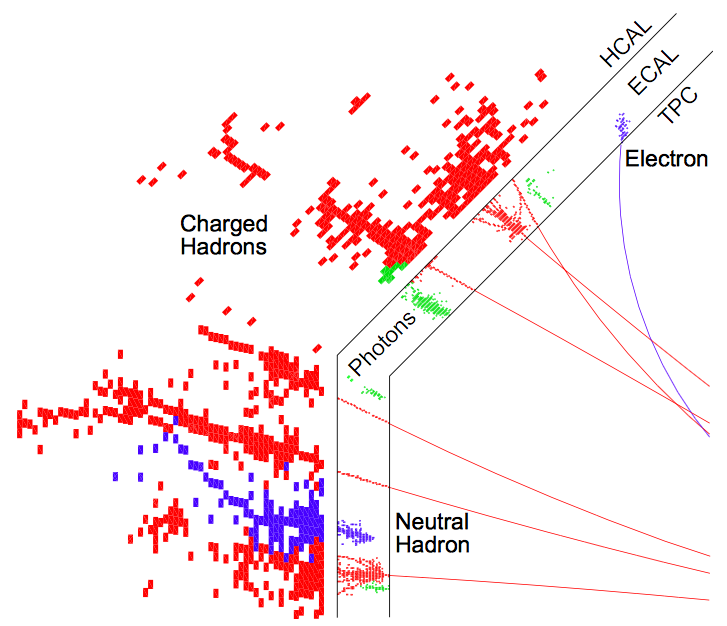
\includegraphics[width=0.5\textwidth]{LCDetectorsAndPFlow/Plots/Pictures/PFlow.png}
\caption[A typical simulated 250 GeV jet in the CLIC\_ILD detector, with labels identifying constituent particles.  Image taken from  \cite{arXiv:1209.4039}.]{A typical simulated 250 GeV jet in the CLIC\_ILD detector, with labels identifying constituent particles.  Image taken from  \cite{arXiv:1209.4039}.}
\label{fig:particleflowpic}
\end{figure} 

%========================================================================================
%========================================================================================

\section{International Large Detector}
\label{sec:ild}
The current detector concepts for the linear collider experiments have been designed to make particle flow calorimetry possible.  While there are a number of different concepts that are under consideration for both the ILC and CLIC, one of the most prominent, and the focus of this work, is the International Large Detector (ILD).  The ILD detector, shown in figure \ref{fig:ild}, achieves very high spatial resolution for all sub-detector systems thanks to its highly segmented calorimeters and central tracking system, both of which are encompassed within a 3.5 T magnetic field.  The sophisticated pattern recognition software that is needed for particle flow calorimetry is provided by PandoraPFA \cite{arXiv:1209.4039, arXiv:0907.3577}.   

\begin{figure}[h!]
\centering
\subfloat[]{\label{fig:ild1}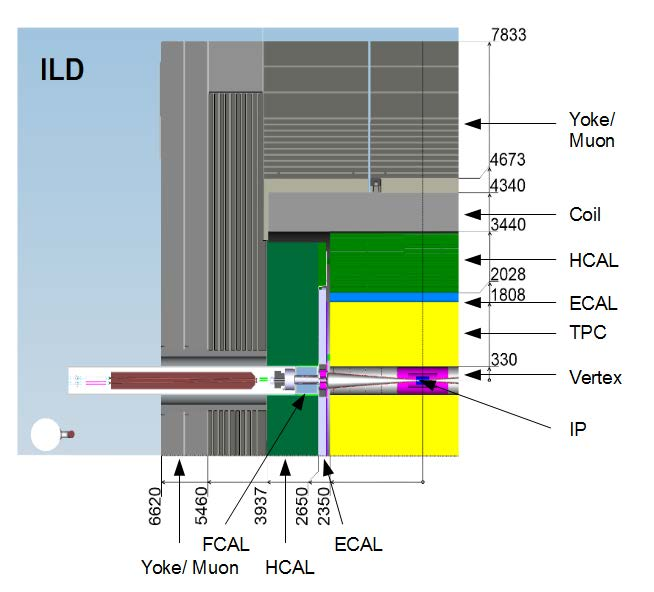
\includegraphics[width=0.5\textwidth]{LCDetectorsAndPFlow/Plots/Pictures/ILD.jpg}}
\subfloat[]{\label{fig:ild2}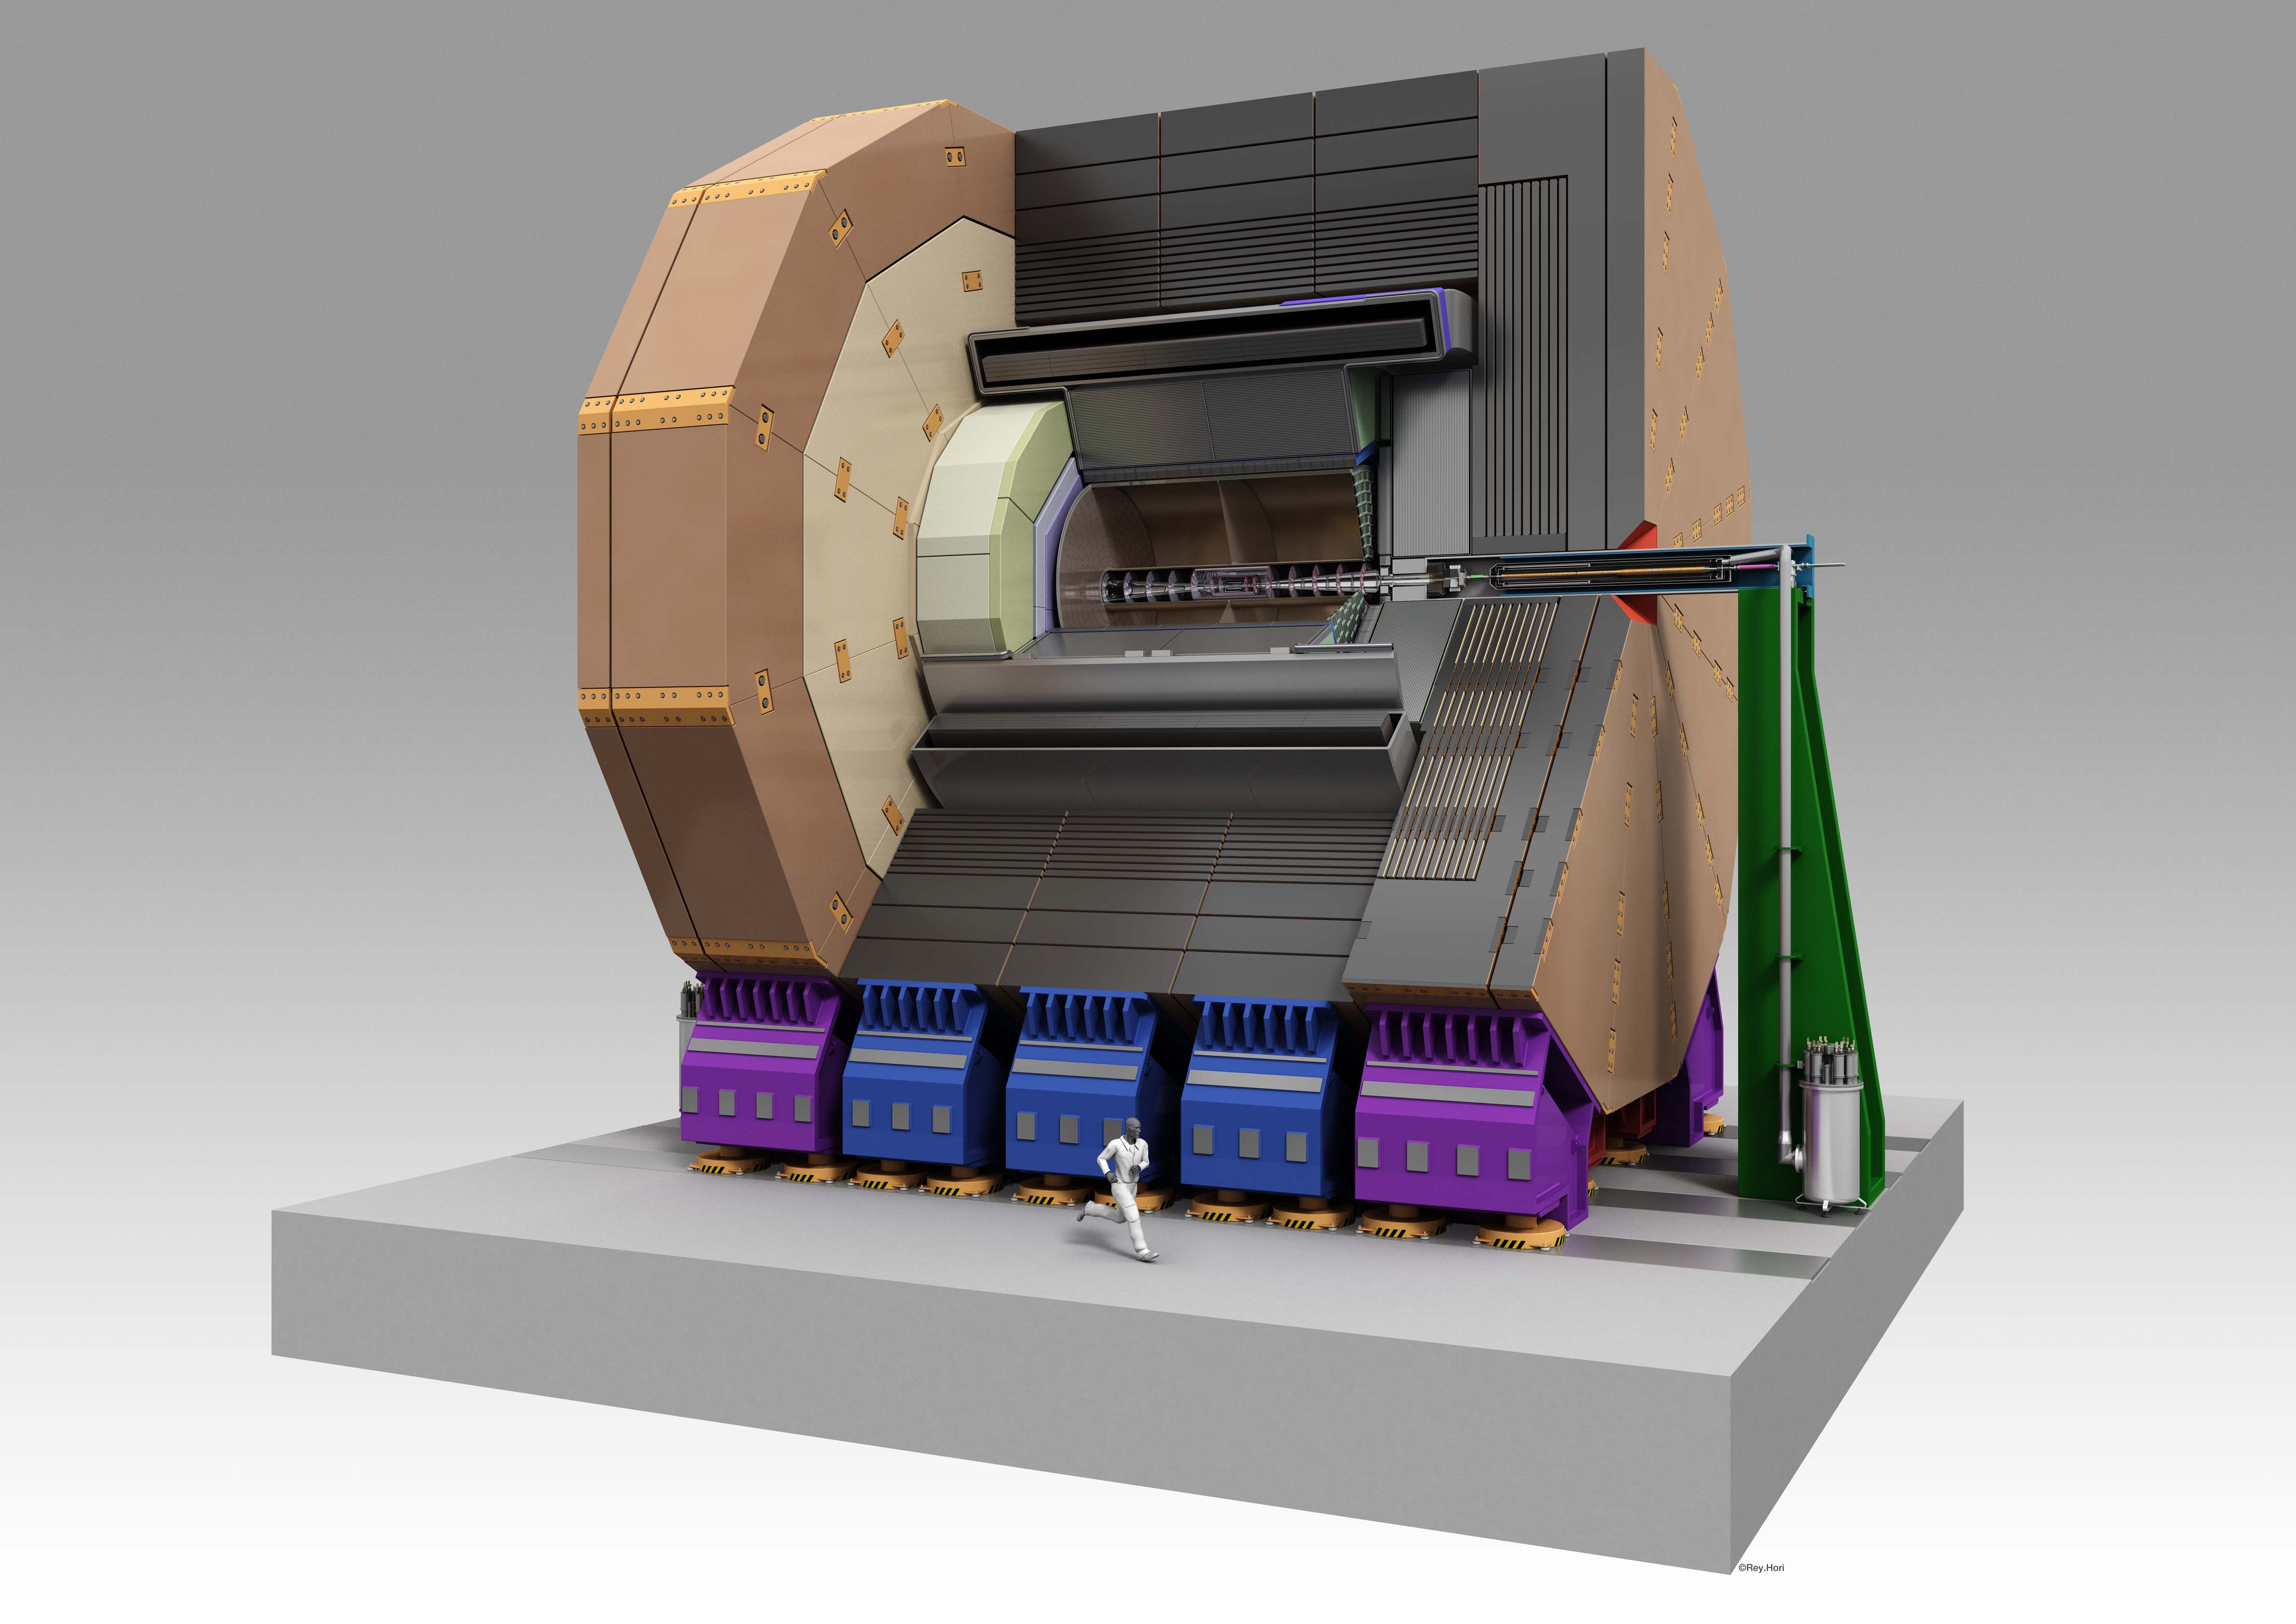
\includegraphics[width=0.5\textwidth]{LCDetectorsAndPFlow/Plots/Pictures/ILD_2.jpg}}
\caption[\protect\subref{fig:ild1} Quadrant view of the ILD detector concept.  The interaction point is in the lower right corner of the picture.  Dimensions are in~mm.  \protect\subref{fig:ild2} An artistic view of the ILD detector concept.  Figures taken from  \cite{Behnke:2013lya}.]{\protect\subref{fig:ild1} Quadrant view of the ILD detector concept.  The interaction point is in the lower right corner of the picture.  Dimensions are in~mm.  \protect\subref{fig:ild2} An artistic view of the ILD detector concept.  Figures taken from  \cite{Behnke:2013lya}.}
\label{fig:ild}
\end{figure} 

%========================================================================================

\subsection{Overview}
The tracking system for the ILD detector consists of a vertex detector, a Time Projection Chamber (TPC) and a number of supplementary silicon detectors.  The vertex detector is designed to give precise information about displaced vertices with respect to the impact point (IP), which is crucial for the study of short lived particles such as the \PD and \PB mesons.  The vertex detector is located close to the IP and surrounding it is the TPC, which is the central tracker for ILD.  The TPC provides detailed measurements of the trajectory of charged particle tracks passing through it, up to 224 measurements per track.  This information is used for determining the curvature of the charged particle track and hence the momentum of the charged particle that transversed it.  Finally, the purpose of the supplementary silicon detectors is to provide additional, high precision, spatial measurements to aid track fitting and extend coverage of the detector down to low polar angles.  

The calorimetric system for ILD is comprised of an electromagnetic calorimeter (ECal), a hadronic calorimeter (HCal) and a number of forward calorimeters (FCal).  The primary function of the ECal is to induce electromagnetic particles to shower within it and to measure the energy of these particle showers.  Similarly, the HCal is designed to induce and measure the energy of hadronic particle showers.  The ECal surrounds the tracking system in the ILD detector and is itself surrounded by the HCal.  The function of FCal is to extend the coverage of the calorimeter system to low polar angles and to provide measurements of the luminosity of the colliding $\text{e}^{\pm}$ beams.  

The outermost elements of the ILD detector are the solenoid, iron yoke and muon system.  The solenoid generates a magnetic field of 3.5~T, which is essential for determining the energy of charged particles in the particle flow paradigm.  The iron yoke is used to return the magnetic field generated by the solenoid.  The yoke is instrumented by the muon system to provide additional information, which supplements the calorimetric energy measurements made by the ILD calorimeters.  

%========================================================================================

\subsection{Vertex Detector}
The main goal of the ILD vertex detector is to achieve a resolution on the impact parameter of charged particle tracks of
\begin{equation}
\sigma_{b} < 5 \oplus \frac{10}{p\text{sin}(\theta)^{3/2}} \text{ {\mu}m,}
\end{equation}
\noindent where $\sigma_{b}$ is the resolution on the track impact parameter, $p$ is the momentum of the track and $\theta$ is the angle between the track and the vertex detector plane.  The first term in this parameterisation is the transverse impact parameters resolution and the second is a multiple-scattering term.  This makes precisely tagging secondary vertices from charm and bottom mesons possible.  Typically these mesons have relatively short proper lifetimes, $\tau$, such that $c\tau \approx \mathcal{O}(300 \text{{ \mu}m})$.  To achieve this impact parameter resolution, a spatial resolution of better than 3~{\mu}m is required near the impact point (IP).  Furthermore, a low material budget of less than 0.15~\% of a radiation length per layer is required to ensure that few electromagnetic showers are initiated within the vertex detector.  A low pixel occupancy is essential for determining the trajectory of individual tracks in the detector.  Furthermore, consideration will have to be given to the mechanical structure of the detector, power consumption and cooling.  

There are a number of different pixel technology options under consideration for the vertex detector for the ILD detector.  This is an active area of ongoing research and development for the linear collider collaboration.  The current design of the vertex detector consists of three concentric layers of double-sided ladders with the first layer contains 10 ladders, the second 11 ladders and the third 17 ladders as shown in figure \ref{fig:vertexpicture}.  Each ladder has two silicon pixel sensors on each side and the ladder thickness is approximately 2~mm.  The radii covered by the detector range from 16~mm to 60~mm from the IP.

\begin{figure}[h!]
\centering
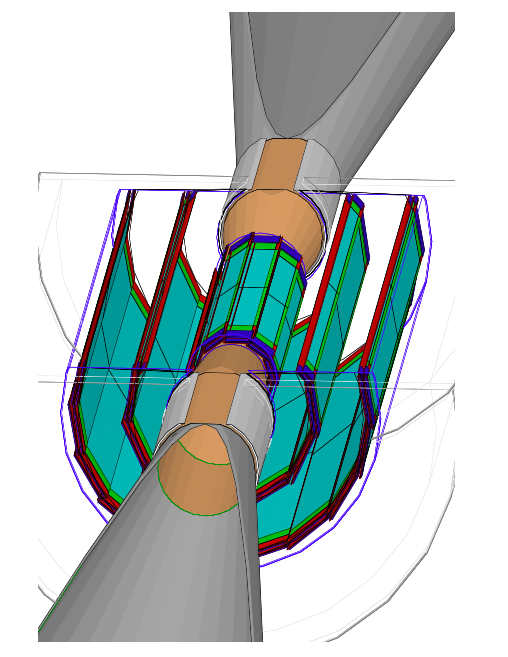
\includegraphics[width=0.3\textwidth]{LCDetectorsAndPFlow/Plots/Pictures/Vertex3.png}
\caption[Vertex detector design for ILD.  Figures taken from \cite{arXiv:1006.3396}.]{Vertex detector design for ILD.  Figures taken from \cite{arXiv:1006.3396}.}
\label{fig:vertexpicture}
\end{figure} 

%========================================================================================

\subsection{Time Projection Chamber}
The central tracking system for the ILD detector is a TPC, which is shown in figure \ref{fig:tracker}.  The TPC consists of a cylindrical gas volume with a central electrode providing an axial electric field.  When a charged particle passes through the TPC, it ionises the gas and the ionised molecules drift in the axial electric field.  The direction of the electric field is chosen such that the electrons drift towards the endplates where they are collected.  The position of the ionisation point can then be calculated using the drift time of the electrons in the TPC.  Combining these TPC hits together makes reconstruction of the full charged particle track possible.  TPCs have an advantage over silicon tracking in that they continuously track any charged particle passing through them, while silicon detectors are only sensitive within each silicon layer.  This compensates for the worse single point resolution that TPCs have in comparison to silicon detectors and makes TPCs a viable option for the ILD detector.  Furthermore, TPCs have a very low material budget.  This benefits calorimetry as it minimises energy losses prior to the particle energy entering the calorimeters, which means the calorimetric energy deposits give a better reflection of the true particle energy.  

The ILD TPC has a point resolution of better than 100~{\mu}m and a double hit resolution in $\phi$ of less than 2~mm.  The gas used for the TPC will be Ar:$\text{CH}_4$:$CO_{2}$ (95:3:2) \cite{Abe:2010aa}.  Several readout technology options, designed to measure the ionisation current, are currently under development.  For all potential options it is envisaged that the readout pads would be $\approx 1 \times 6 \text{mm}^{2}$ giving a total of approximately $10^{6}$ pads on each TPC endplate.

\begin{figure}[h!]
\centering
\subfloat[]{\label{fig:tracker1}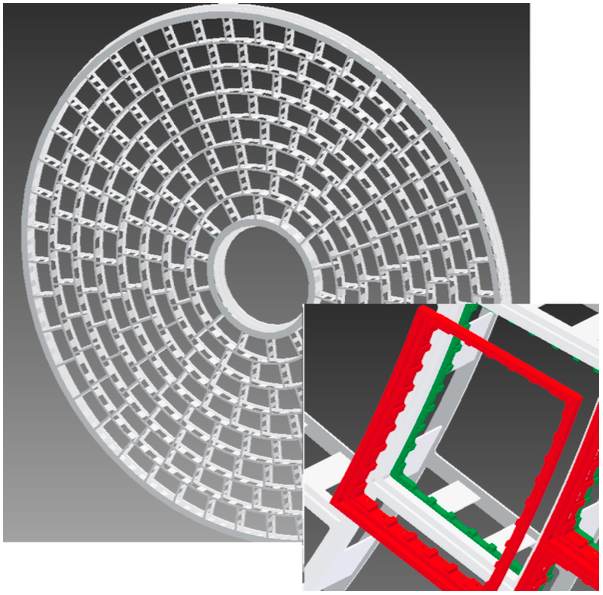
\includegraphics[width=0.5\textwidth]{LCDetectorsAndPFlow/Plots/Pictures/Tracker1.png}}
\subfloat[]{\label{fig:tracker2}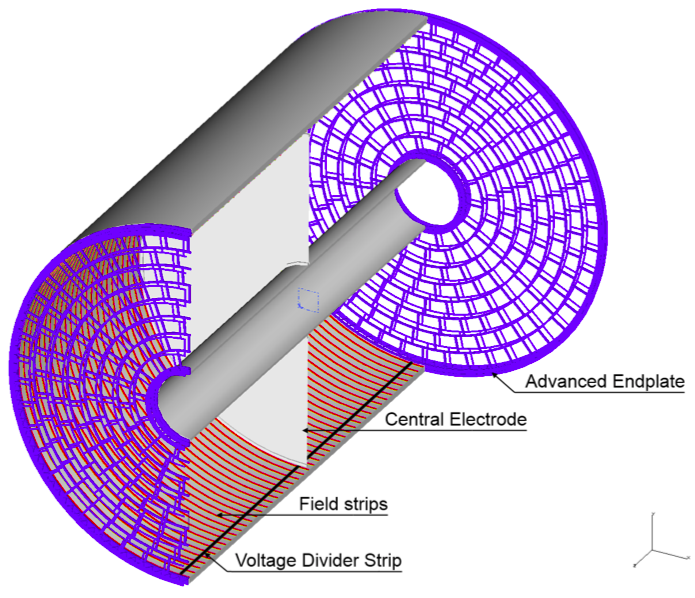
\includegraphics[width=0.5\textwidth]{LCDetectorsAndPFlow/Plots/Pictures/Tracker2.png}}
\caption[\protect\subref{fig:tracker1} Drawing of the proposed end-plate for the TPC.  In the insert a back frame, which is designed to support the readout modules, is shown.  \protect\subref{fig:tracker2} Conceptual sketch of the TPC system showing the main parts of the TPC (not to scale).  The central electrode generates the axial electric field, the endplates collect the ionisation electrons, the field strips help to maintain a uniform electric field across the TPC and the voltage divider strips maintains the voltage difference between the anode and cathode.  The field strips are held at fixed voltages such that they replicate the electric filed produced by the electrodes.  This reinforcing of the electric field configuration minimises non-uniformities in the electric field.  The field cage of the TPC is not shown.]{\protect\subref{fig:tracker1} Drawing of the proposed end-plate for the TPC.  In the insert a back frame, which is designed to support the readout modules, is shown.  \protect\subref{fig:tracker2} Conceptual sketch of the TPC system showing the main parts of the TPC (not to scale).  The central electrode generates the axial electric field, the endplates collect the ionisation electrons, the field strips help to maintain a uniform electric field across the TPC and the voltage divider strips maintains the voltage difference between the anode and cathode.  The field strips are held at fixed voltages such that they replicate the electric filed produced by the electrodes.  This reinforcing of the electric field configuration minimises non-uniformities in the electric field.  The field cage of the TPC is not shown.}
\label{fig:tracker}
\end{figure} 

%========================================================================================

\subsection{Supplemental Silicon Tracking System}
There are four components that make up the supplemental silicon tracking system in ILD, shown in figure \ref{fig:vertex}, which are:
\begin{itemize}
\item Silicon Inner Tracker (SIT) and Silicon External Tracker (SET).  These are both barrel components, which are positioned immediately inside and outside the TPC.  The SIT helps form associations between hits in the vertex detector and TPC, while the SET helps with extrapolation of TPC tracks into the calorimeter.  
\item Endplate of the TPC (ETD).  This sensor is identical to the SET, but is positioned in front of the ECal endcap calorimeter.  The ETD extends the coverage of the supplemental silicon tracking system envelope. 
\item Forward tracker (FTD).  This detector consists of seven silicon disks that extend the coverage of the tracking down to small angles that are not covered by the TPC.  
\end{itemize}

\begin{figure}[h!]
\centering
\subfloat[]{\label{fig:vertex1}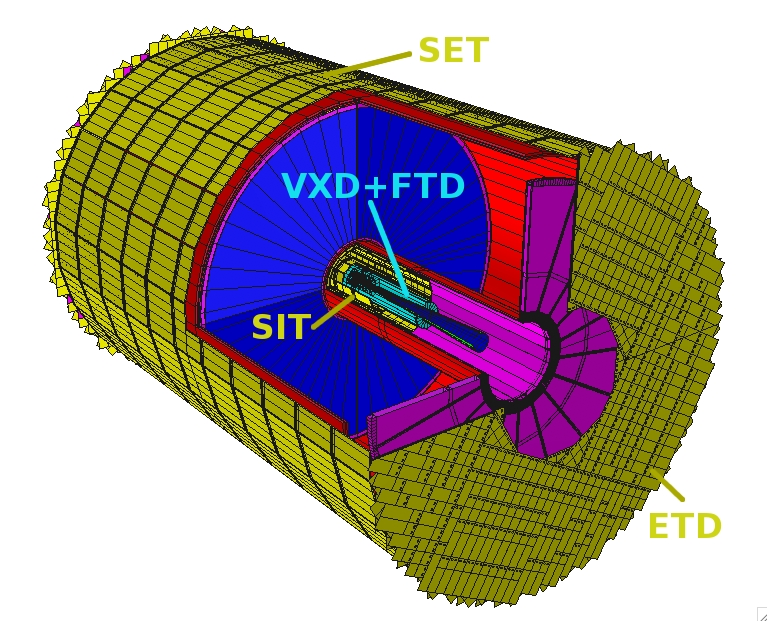
\includegraphics[width=0.5\textwidth]{LCDetectorsAndPFlow/Plots/Pictures/Vertex1.jpg}}
\subfloat[]{\label{fig:vertex2}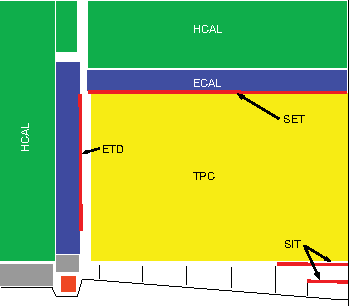
\includegraphics[width=0.5\textwidth]{LCDetectorsAndPFlow/Plots/Pictures/Vertex2.pdf}}
\caption[\protect\subref{fig:vertex1} A 3D detailed GEANT4 simulation description of the silicon system.  \protect\subref{fig:vertex2} A quadrant view of the ILD silicon envelope made of the four components SIT, SET, ETD and FTD as included in the full MOKKA simulation.  Figures taken from  \cite{Behnke:2013lya}.]{\protect\subref{fig:vertex1} A 3D detailed GEANT4 simulation description of the silicon system.  \protect\subref{fig:vertex2} A quadrant view of the ILD silicon envelope made of the four components SIT, SET, ETD and FTD as included in the full MOKKA simulation.  Figures taken from  \cite{Behnke:2013lya}.}
\label{fig:vertex}
\end{figure} 

\begin{table}[h!]
\centering
\begin{tabular}{ l r}
\hline
Tracking System & Coverage [cos$\theta$] \\
\hline
SIT & 0.910 \\
SET & 0.789 \\
ETD & 0.799 - 0.985 \\
FTD & 0.802 - 0.996\\
\hline
\end{tabular}
\caption[Coverage of the supplementary silicon tracking systems in the ILD detector.  In this table $\theta$ is the polar angle with respect to the beam direction.  Taken from \cite{Behnke:2013lya}.]{Coverage of the supplementary silicon tracking systems in the ILD detector.  In this table $\theta$ is the polar angle with respect to the beam direction.  Taken from \cite{Behnke:2013lya}.}
 \label{table:supptrackingcoverage}
\end{table}

The coverage of the SIT, SET, ETD and FTD is given in table \ref{table:supptrackingcoverage}.  These detectors are designed to give high precision space points that can be used in track fitting.  Furthermore, the ETD and SET are of particular use for extrapolating the charged particle tracks into the calorimeters.  This is key for particle flow calorimetry, which relies upon correct association of charged particle tracks and clusters of calorimeter hits.  Analogously to the vertex detector, these detectors require low material budget and low occupancy.  The FTD, due to its proximity to the beam axis, is particularly prone to high occupancies.  

The SIT, SET and ETD are silicon pixel sensors with 50~{\mu}m pitch embedded in 200~{\mu}m thick silicon.  The FTD consists of seven silicon tracking disks, the first two being pixel detectors and the remaining five being strip detectors.  The pixel detector disks are formed of 16 petals, as shown in figure \ref{fig:ftd}.  Within these petals the pixel size varies from $26 \times 29~{\mu}\text{m}^{2}$ to $26 \times 67~{\mu}\text{m}^{2}$.  Strip detectors are used for the outermost tracking disks as the occupancy considerations do not demand a high granularity detector i.e. a pixel detector.  These detector disks will have a pitch of 50~{\mu}m.  The active sensor and readout ASIC design for each of these detectors is an active area of development for the linear collider.  

\begin{figure}[h!]
\centering
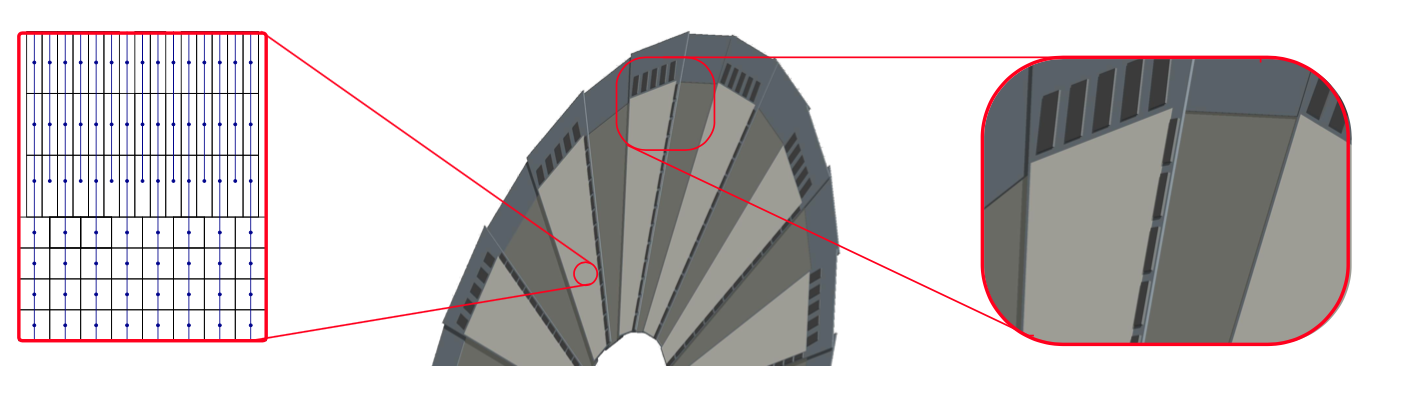
\includegraphics[width=0.8\textwidth]{LCDetectorsAndPFlow/Plots/Pictures/FTD.png}
\caption[A half-disk for the FTD showing the petal concept.  The rightmost zoom image showers a detail of the end-of-petal area that houses the read-out electronics.  The leftmost image shows the region at $R = 8$~cm where both the column width and the $R$-dimension of the pixels changes.  Figures taken from \cite{Behnke:2013lya}.]{A half-disk for the FTD showing the petal concept.  The rightmost zoom image showers a detail of the end-of-petal area that houses the read-out electronics.  The leftmost image shows the region at $R = 8$~cm where both the column width and the $R$-dimension of the pixels changes.  Figures taken from \cite{Behnke:2013lya}.}
\label{fig:ftd}
\end{figure} 

%========================================================================================

\subsection{Electromagnetic Calorimeter}
\label{sec:ildecal}
The nominal ILD detector contains a finely segmented electromagnetic sampling calorimeter (ECal).  The ILD ECal has been specifically designed with particle flow calorimetry in mind.  To that extent the spatial resolution of particle showers within the ECal takes as much, if not more, precedence than the energy resolution.   

There are a number of design requirements for the ECal:
\begin{itemize}
\item The ECal must be compact in size to reduce the overall cost of the detector.
\item Fine segmentation of the ECal is required so that nearby particle showers can be separated.  This is an essential requirement for particle flow calorimetry.
\item Electromagnetic showers should be contained within the ECal.
\end{itemize}
Based on these requirements tungsten is used as the absorber material for the ILD ECal as it has a small radiation length ($X_{0}$), a small Moli�re radius and a large ratio of radiation length to nuclear interaction length.  A comparison of these properties for other ECal absorber material candidates is shown in table \ref{table:absorberoptions}.  The small radiation length in tungsten allows for a large number of radiation lengths, $\approx 24 X_{0}$, to be compacted within a relatively short distance, $\approx 20$ cm, in nominal ILD ECal.  This is sufficient for containing all but the highest energy electromagnetic showers.  The small Moli�re radius in tungsten will lead to compact electromagnetic showers.  This makes separation of nearby showers easier.  Finally, the large ratio of the radiation length to the nuclear interaction length in tungsten will lead to greater longitudinal separation between electromagnetic and hadronic showers again making shower identification easier.   

The active material in the nominal ILD ECal is silicon, however, a scintillator strip option is also being considered.  It contains a total of 30 longitudinal readout layers, which is sufficient to provide a good energy resolution.  The tungsten thickness for the innermost 20 layers is 2.1~mm, while for the final 10 layers it is 4.2~mm.  This configuration of absorber material thickness is chosen to reduce the number of readout channels and hence the cost, while maintaining a high sampling rate for particle showers at the start of the ECal.  It should be noted that this ECal offers no gains in terms of energy resolutions in comparison to preexisting particle collider experiments, as shown in table \ref{table:ecalenergyres}.  This is the case because the focus of this calorimeter is split between imaging the particle showers and recording their energy as opposed to purely focusing on the energy measurement.  Each of the ECal layers is divided up into square cells, of side length 5~mm, which makes separation of nearby particle showers possible.  This cell size was chosen as a balance between being able to resolve nearby particle showers and reducing the overall cost of the calorimeter, which scales with the number of readout channels.  An optimisation study of the various ECal parameters for the ILD detector can be found in section \ref{sec:ecal}.

\begin{table}[h!]
\centering
\begin{tabular}{ l l l l l}
\hline
Material & $\lambda_{I}$ (cm) & $X_{0}$ (cm) & $\rho_{M}$ (cm) & $ \frac{\lambda_{I}}{X_{0}}$ \\
\hline
Fe & 16.8 & 1.76 & 1.69 & 9.5 \\
Cu & 15.1 & 1.43 & 1.52 & 10.6 \\
W & 9.6 & 0.35 & 0.93 & 27.4 \\
Pb & 17.1 & 0.56 & 1.00 & 30.5 \\
\hline
\end{tabular}
\caption[Comparison of the nuclear interaction length $\lambda_{I}$, radiation length $X_{0}$ and Moli�re radius for iron, copper, tungsten and lead.  Table taken from \cite{arXiv:0907.3577}.]{Comparison of the nuclear interaction length $\lambda_{I}$, radiation length $X_{0}$ and Moli�re radius for iron, copper, tungsten and lead.  Table taken from \cite{arXiv:0907.3577}.}
\label{table:absorberoptions}
\end{table}

\begin{table}[h!]
\centering
\begin{tabular}{ l l }
\hline
Experiment & ECal Energy Resolution $\frac{\sigma_{E}}{E}$ \\
\hline
CMS \cite{Chatrchyan:2013dga} & $\sim \frac{2.8\%}{\sqrt{E(\text{GeV})}} \oplus 0.3\% \oplus \frac{12\%}{E(\text{GeV})}$ \\
ATLAS \cite{Aharrouche:2006nf} & $\sim \frac{10.1\%}{\sqrt{E(\text{GeV})}} \oplus 0.1\%$ \\
LHCb \cite{Perret:2014owa} & $\sim \frac{9\%}{\sqrt{E(\text{GeV})}} \oplus 0.8\%$ \\
ILC (ILD Silicon Option) \cite{Behnke:2013lya} & $\sim \frac{16.6\%}{\sqrt{E(\text{GeV})}} \oplus 1.1\%$ \\
\hline
\end{tabular}
\caption[Comparison of the ECal energy resolutions for various experiments.]{Comparison of the ECal energy resolutions for various experiments.}
\label{table:ecalenergyres}
\end{table}

\begin{figure}[h!]
\centering
\subfloat[]{\label{fig:ecalimage1}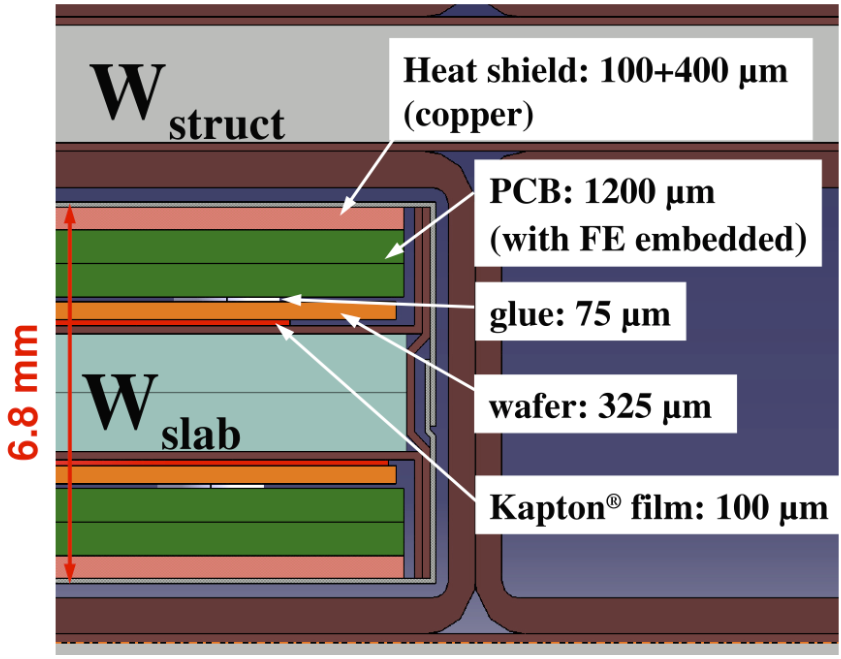
\includegraphics[width=0.4\textwidth]{LCDetectorsAndPFlow/Plots/Pictures/SiECal.png}} 
\hspace{1cm}
\subfloat[]{\label{fig:ecalimage2}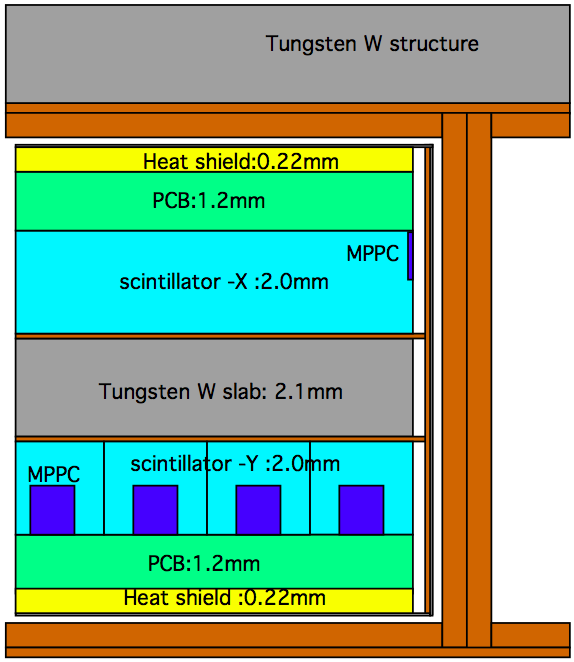
\includegraphics[width=0.4\textwidth]{LCDetectorsAndPFlow/Plots/Pictures/ScECal.png}}
\caption[Cross section through ECal layer for \protect\subref{fig:ecalimage1} silicon and \protect\subref{fig:ecalimage2} scintillator option.  Figures taken from  \cite{Behnke:2013lya}.]{Cross section through ECal layer for \protect\subref{fig:ecalimage1} silicon and \protect\subref{fig:ecalimage2} scintillator option.  Figures taken from  \cite{Behnke:2013lya}.}
\label{fig:ecalimage}
\end{figure} 

%========================================================================================

\subsection{Hadronic Calorimeter}
A finely segmented hadronic sampling calorimeter (HCal) is used in the nominal ILD detector.  The design requirements for the ILD HCal mirror those of the ECal, which can be found in section \ref{sec:ildecal}, with one exception; the HCal is designed to contain hadronic showers as opposed to electromagnetic showers.  Steel is used as the absorber material for the HCal as it has durable mechanical properties that allow the HCal to be constructed without the need of auxiliary supports.  If required, auxiliary supports would create dead regions in the detector that would harm performance.  Furthermore, steel is relatively inexpensive and has a relatively small nuclear interaction length, meaning it is possible to achieve a compact calorimeter design at low cost.  The nominal ILD HCal contains approximately $6 \lambda_{I}$, which when combined with the $1 \lambda_{I}$ in the ECal is enough to contain the majority of hadronic showers at ILC like energies.  

The active material in the nominal ILD HCal is scintillator.  In total, the HCal contains 48 readout layers, which provides an extremely good energy resolution.  This can be seen when comparing the HCal energy resolution between different experiments, as shown in table \ref{table:hcalenergyres}.  An individual layer in the HCal is comprised of 20~mm of steel absorber material with 3~mm of scintillator active material.  Each layer in the HCal is segmented into square cells, of side length 30~mm.  This cell size was chosen as a balance between reducing the cost of the detector, which is proportional to the number of readout channels, and achieving the required spatial resolution to make particle flow calorimetry possible.  The segmentation of the ILD HCal gives excellent spatial resolution and sufficiently good energy resolution to make the use of particle flow calorimetry a reality.  An optimisation study of the various HCal parameters for the ILD detector can be found in section \ref{sec:hcal}.

The ILD HCal is intrinsically non-compensating, which means that it has a different response to electromagnetic and hadronic showers.  The origin of this different response is the fundamentally different mechanisms governing the propagation of electromagnetic and hadronic showers.  One key difference between the mechanisms is that hadronic showers have an invisible energy component, which occurs due to  effects such as neutrons coming to rest in the detector and nuclear biding energy losses \cite{Tran:2017tgr}.  In general, this leads to a lower response from a calorimeter to a hadronic shower than an electromagnetic shower.  A number of different software techniques have been developed for the linear collider experiment that attempt to correct this non-compensating response.  For more details see chapter \ref{chap:energyestimators}.  The ILD ECal has a compensating response due to the use of tungsten as the absorber material \cite{Blaising:2015nla}, therefore, no additional treatment of energies is required.

\begin{table}[h!]
\centering
\begin{tabular}{ l l }
\hline
Experiment & HCal Energy Resolution $\frac{\sigma_{E}}{E}$ \\
\hline
CMS \cite{Budd:2001eu} & $\sim \frac{90\%}{\sqrt{E(\text{GeV})}} \oplus 4.8\%$ \\
ATLAS \cite{Airapetian:1996iv} & $\sim \frac{52.1\%}{\sqrt{E(\text{GeV})}} \oplus 3.0\% \oplus \frac{1.6\%}{E(\text{GeV})}$ \\
LHCb \cite{Perret:2014owa} & $\sim \frac{69\%}{\sqrt{E(\text{GeV})}} \oplus 9.0\%$ \\
ILC (ILD Silicon Option) \cite{Behnke:2013lya} & $\sim \frac{43.3\%}{\sqrt{E(\text{GeV})}} \oplus 1.8\%$ \\
\hline
\end{tabular}
\caption[Comparison of the HCal energy resolutions for various experiments.]{Comparison of the HCal energy resolutions for various experiments.}
\label{table:hcalenergyres}
\end{table}

%========================================================================================

\subsection{Solenoid, Yoke and Muon System}
Surrounding the ILD calorimeter system is solenoid that generates a 3.5~T magnetic field.  The magnetic field produced by the coil is crucial for bending charged particles so that their momentum can be determined from the curvature of the path they transverse.  Furthermore, the bending of charged particles leads to greater separation of calorimetric energy deposits between charged and neutral particles, which will reduce the effects of confusion when using particle flow calorimetry.  

The magnetic field in the ILD detector is returned by an iron yoke that surrounds the solenoid.  Iron is chosen for the yoke material as it has a very large permeability.  

This yoke is instrumented by a muon system in the barrel and forward regions of the detector.  The goal of this instrumentation is to identify muons escaping the calorimeters and to act as a tail catcher for the calorimeters.  The muon system consists of 10 layers, spaced 140~mm apart, followed by 2 (3) layers spaced 600~mm apart in the barrel (endcap) region of the detector, as shown in figure \ref{fig:muon}.  There is also an additional sensitive layer for the barrel region placed immediately outside the HCal to help with association energy deposits between the calorimeters and the yoke.  As the majority of particles at ILC like energies will be contained within the calorimeters, the energy and spatial resolution of the muon system are not critical to performance.  It is for that reason that the number of layers is lower and the layer thicknesses wider in the yoke than in the calorimeters.  The nominal ILD model uses 30~mm wide and 1 m long scintillator strips as the readout technology for the yoke.

\begin{figure}[h!]
\centering
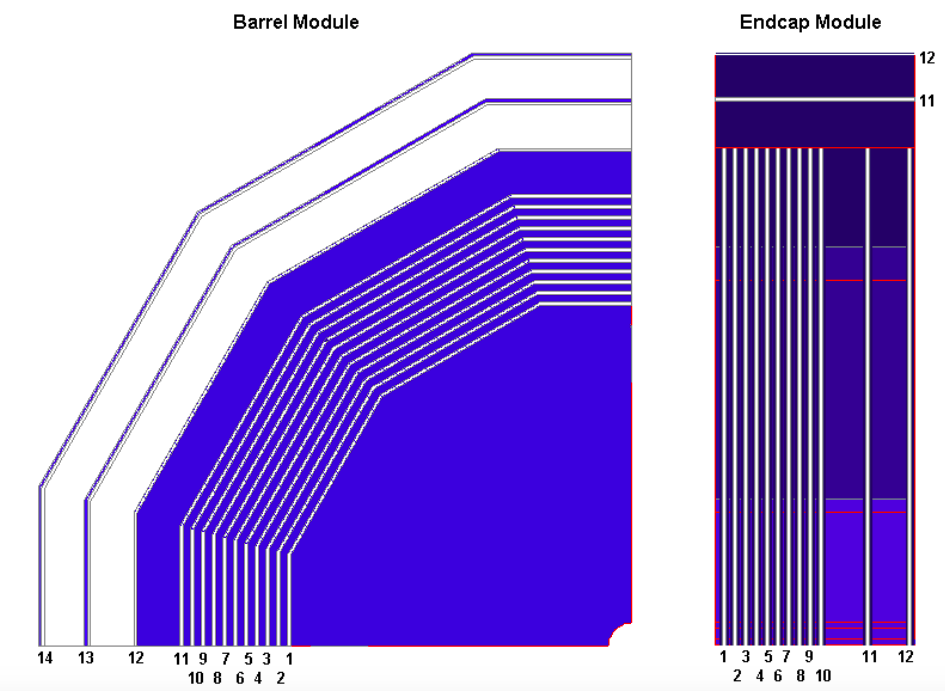
\includegraphics[width=0.5\textwidth]{LCDetectorsAndPFlow/Plots/Pictures/Muon.png}
\caption[The sensitive layers of the ILD muon system.  Figure taken from  \cite{Behnke:2013lya}.]{The sensitive layers of the ILD muon system.  Figure taken from  \cite{Behnke:2013lya}.}
\label{fig:muon}
\end{figure}   

%========================================================================================

\subsection{Forward Calorimetry}
Forward calorimetry in the ILD detector consists of three additional sampling calorimeters:
\begin{itemize}
\item The LumiCal, which is located within the octagonal hole in the ECal endcap.  This will give a precise measurement of the luminosity of the linear collider beam.   The LumiCal uses Bhabha scattering, $\text{e}^{+}\text{e}^{-} \rightarrow \text{e}^{+}\text{e}^{-}(\gamma)$, as a gauge process for the luminosity measurement.  Using this approach the luminosity can be measured with precision of less than $10^{-3}$ at $\sqrt{s}=500$~GeV \cite{Abe:2010aa}. 
\item The LHCal, which is positioned within the square hole of the HCal endcap.  This hadronic calorimeter is designed to extend the coverage of the HCal down to small polar angles.  
\item The BeamCal, which is located just in front of the final focusing quadrupole.  This calorimeter will perform a bunch-by-bunch estimate of the luminosity based on the energy deposited in the calorimeter.
\end{itemize}
The layout of these calorimeters is shown in figure \ref{fig:fcal} and their coverage is summarised in table \ref{table:fcalcoverage}.  Each of the forward calorimeters will have to deal with high occupancies due to the presence of background processes, e.g. beamstrahlung, which makes fast readout crucial.  Furthermore, the BeamCal experiences a large flux of low energy electrons due to its proximity to the beam pipe, which results in a large radiation dose.  This makes radiation hard sensors essential for the BeamCal.  

\begin{figure}[h!]
\centering
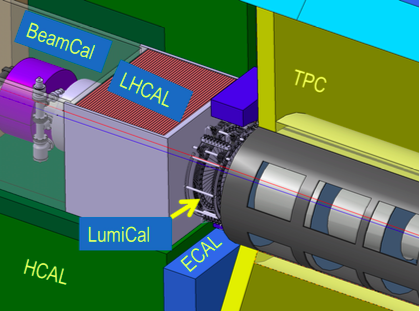
\includegraphics[width=0.5\textwidth]{LCDetectorsAndPFlow/Plots/Pictures/FCal.png}
\caption[The very forward region of the ILD detector.  LumiCal, BeamCal and LHCal are carried by the support tube for the final focusing quadruple, QD0, and the beam pipe.  Figure taken from  \cite{Behnke:2013lya}.]{The very forward region of the ILD detector.  LumiCal, BeamCal and LHCal are carried by the support tube for the final focusing quadruple, QD0, and the beam pipe.  Figure taken from  \cite{Behnke:2013lya}.}
\label{fig:fcal}
\end{figure} 

\begin{table}[h!]
\centering
\begin{tabular}{ l r }
\hline
Forward Calorimeter & Polar Angle Coverage [mrad] \\
\hline
LumiCal & $31 - 77$ \\
LHCal & $\sim 29 - 122$ \\
BeamCal & $5 - 40$ \\
\hline
\end{tabular}
\caption[Coverage of the forward calorimeters in the ILD detector.]{Coverage of the forward calorimeters in the ILD detector.}
\label{table:fcalcoverage}
\end{table}

Each of these forward calorimeters is constructed using tungsten as the absorber material.  The small Moli�re radius of tungsten ensures that narrow electromagnetic showers are formed within them, which makes separation and identification of showering particles easier.  

The layout of these calorimeters is as follows:
\begin{itemize}
\item The LumiCal is a silicon tungsten sampling calorimeter that contains 30 readout layers.  This gives the LumiCal a total depth of $\approx 24 X_{0}$.  
\item The LHCal is also a silicon tungsten sampling calorimeter, which contains 40 readout layers.  The total depth of the LHCal is $\approx 4 \lambda_{I}$.
\item The BeamCal is a tungsten based sampling calorimeter.  The sensitive detector material for the BeamCal is an ongoing area of research as, due to the extremely high occupancy from the beam induced backgrounds, a very fast readout is required.  The exact layer configuration of the BeamCal will depend upon the choice of sensitive detector material and hence is yet to be specified.  
\end{itemize}
The segmentation within the layers, the cell size, in these forward calorimeter is yet to be fully optimised.

%========================================================================================

\section{Simulation}
\label{sec:simulation}
Detector model simulation for all studies presented in this work was performed using MOKKA \cite{MoradeFreitas:2002kj}, a GEANT4 \cite{Agostinelli:2002hh} wrapper providing detailed geometric descriptions of detector concepts for the linear collider.  The MOKKA simulation of the ILD detector contains the following \cite{Behnke:2013lya}:
\begin{itemize}
\item The vertex detector is simulated using silicon as the sensitive material.  Support material and the cryostat are also included.
\item The supplementary silicon tracking systems are included.  Again, material has been added to the simulation to represent the support material for these systems.  Furthermore, an estimation has been made of the material budget for power and readout cables from the vertex detector, SIT and FTD and material has been added to the simulation to represent these.  The material added to represent the power and readout cables comes in the form of an aluminium cylinder running inside the TPC field cage and around a cone around the beam pipe.
\item The TPC is simulated as a cylindrical volume of a gas mixture surrounded by a field cage.  A conservative estimate of the endplate is included in the simulation to account for the support structure, electronics and cooling pipes for the TPC.
\item As well as including the silicon tungsten sampling calorimeter, the simulation of the ILD ECal contains additional material to represent the instrumented region of the sensor and a heat shield as shown in figure \ref{fig:ecalimage}.
\item Simulation of the ILD HCal has a number of realistic features including detailed modelling of the electronics, detector gaps and the implementation of Birk's law \cite{Birks:1951boa} for the scintillator sensitive detector elements.
\item The muon system, which is the instrumentation of the iron yoke, uses scintillator as the active material in the simulation.  A square cell size of side length 30~mm is assumed.  This is in contrast to the nominal ILD model, but as the tail-catcher plays a minimal role in event reconstruction at ILC like energies this difference should have negligible impact.  
\item The forward calorimeters, the LumiCal, LHCal and BeamCal, are all included in the simulation.  Tungsten is used as the absorber material for each of the calorimeters.  The LumiCal and LHCal use a silicon readout material, while the BeamCal uses a diamond readout.  
\end{itemize}

%========================================================================================

%\section{Reconstruction Chain}

%\section{Event Generation, Simulation and Reconstruction}

%The jet fragmentation and hadronisation for the Z $\rightarrow$ uds events used for determining the metric for detector performance was controlled using PYTHIA \cite{Sjostrand:2006za} that had been tuned using data from LEP \cite{Alexander:1995bk}.  Single particle spatially isotropic samples of $K_{L}^{0}$, $\gamma$ and $\mu^{-}$ were produced for the calibration of each detector model.  A simple c++ script was written to generate the relevant HEPEvt common blocks for these samples. 

%Event reconstruction was performed using MARLIN \cite{Gaede:2006pj}, a c++ framework designed for reconstruction at the linear collider.  PandoraPFA \cite{arXiv:0907.3577, arXiv:1209.4039} was used to apply Particle Flow Calorimetry in the reconstruction, the full details of which can be found in chapter PANDORA CHAPTER.

%========================================================================================

\section{CLIC ILD}
The increased collision energy of the proposed CLIC accelerator means the use of the nominal ILD detector model would be inappropriate.  Therefore, a new detector model, CLIC\_ILD \cite{Linssen:2012hp}, based upon the nominal ILD detector model was created to cope with the experimental conditions found at the CLIC experiment.  The main differences between the nominal ILD detector and CLIC\_ILD are:

\begin{figure}[h!]
\centering
\subfloat[]{\label{fig:clicild1}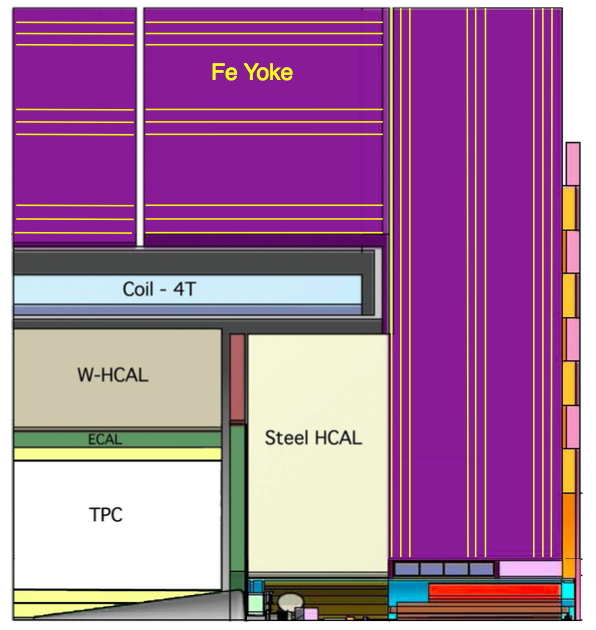
\includegraphics[width=0.4\textwidth]{LCDetectorsAndPFlow/Plots/Pictures/CLIC_ILD.png}}
\hspace{1cm}
\subfloat[]{\label{fig:clicild2}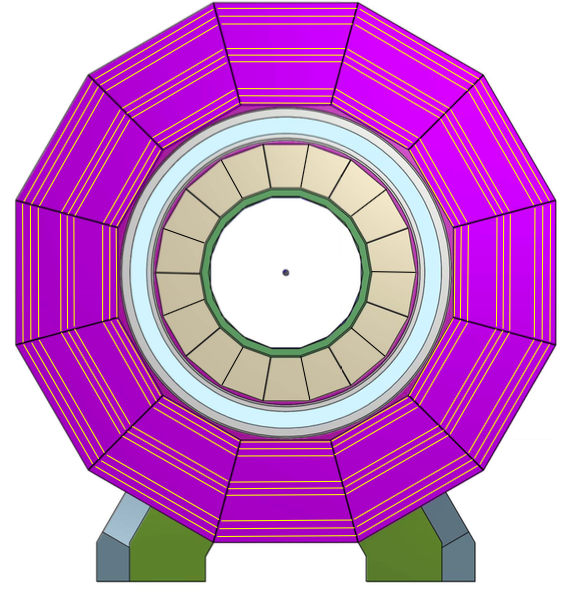
\includegraphics[width=0.4\textwidth]{LCDetectorsAndPFlow/Plots/Pictures/CLIC_ILD_2.png}}
\caption[\protect\subref{fig:ild1} Longitudinal (top quadrant) and \protect\subref{fig:ild2} transverse cross section of the CLIC\_ILD detector.  Figures taken from \cite{Linssen:2012hp}.]{\protect\subref{fig:ild1} Longitudinal (top quadrant) and \protect\subref{fig:ild2} transverse cross section of the CLIC\_ILD detector.  Figures taken from \cite{Linssen:2012hp}.}
\label{fig:clicild}
\end{figure} 

\begin{itemize}
\item The higher energies found at the CLIC experiment lead to more intense beam induced backgrounds, which is especially problematic for detectors close to the IP where the occupancies will be extremely high.  For this reason the inner vertex detector in CLIC\_ILD is moved 15~mm further out from the IP.    
\item The HCal thickness is increased from 6 $\lambda_{I}$ to 7.5 $\lambda_{I}$.  This ensures that higher energy hadronic showers found at the CLIC experiment are contained within the calorimeters.  
\item The HCal absorber material for the barrel is tungsten as opposed to steel.  This reduces the overall thickness of the HCal and keeps the coil size, one of the driving cost factors for the detectors, similar for the nominal ILD and CLIC\_ILD detectors.  Steel is used as the absorber material for the HCal endcaps as there are no spatial requirements relating to the coil size and this will lower the detector cost.  Furthermore, the shower development time in steel is faster than in tungsten making effective time stamping of energy deposits easier, which is crucial for the CLIC experiment for vetoing beam induced backgrounds.  
\item The magnetic field strength in the CLIC\_ILD detector is increased to 4 T.  This was found to benefit the reconstruction, particularly at high energies, as it leads to greater separation of charged particle tracks.  Furthermore, it was possible to achieve this increase in field strength using the nominal ILD coil design.   
\item The CLIC\_ILD detector contains masking, graphite layers placed in front of the BeamCal, to prevent particles produced by the beam-induced interactions from backscattering into the main detector.  It is the increased collision energy that makes backscattering of particles a more problematic effect for the CLIC experiment than it is for the ILC experiment.   
\end{itemize}  

%========================================================================================
%======================================================================================== 

\section{Particle Flow Reconstruction}
\label{sec:reconstruction}
Particle flow calorimetry relies upon correct associations being made between calorimetric energy deposits and charged particle tracks.  Even with a finely segmented detector, such as the ILD detector described in section \ref{sec:ild}, correctly making these associations is a highly a non-trivial task and must be done using advanced pattern recognition software.  This is provided by the PandoraPFA particle flow algorithm \cite{arXiv:0907.3577, arXiv:1209.4039}.  PandoraPFA is applied in the linear collider reconstruction using MARLIN \cite{Gaede:2006pj}, a c++ framework specifically designed for the linear collider.  

%======================================================================================== 

\subsection{PandoraPFA}
PandoraPFA takes as input calorimeter hits and charged particles tracks and produces as output reconstructed particles known as particle flow objects (PFOs).  The pattern recognition in PandoraPFA is applied in eight main stages \cite{arXiv:0907.3577}:
\begin{enumerate}
\item Track selection.  The input track collections are examined to determine whether $V^{0}$ decays, two charged tracks originating from a point displaced from the IP, or kinks, where a charged particle has decayed into a single charged particle and a number of neutral ones, are present.  Such information will be propagated in the reconstruction to the final PFO creation stage.  
\item Calorimeter hit treatment.  The treatment of calorimeter hits by PandoraPFA is of paramount importance to the work presented in chapters \ref{chap:energyestimators} and \ref{chap:detopt}.  Therefore, full details of the calorimeter hit selection procedure are presented here.  This selection procedure is broken down into several steps:
\begin{itemize}
\item The various collection of, post digitisation, calorimeter hits are passed into the Pandora framework and converted into Pandora calorimeter hits.  
\item To minimise any dependancy on the detector geometry each calorimeter hit is assigned to a pseudo-layer, which is representative of the hits position in the calorimeter.  All further topological association algorithms work using the pseudo-layer definition, illustrated in figure \ref{fig:pseudolayer}.  
\item A minimum ionising particle equivalent energy cut is applied to the calorimeter hits.  If a calorimeter hit contains less than 0.5 (0.3) of the energy of a normally incident MIP passing through the calorimeter cell in the ECal (HCal) then it is not used in the reconstruction.  
\item If a calorimeter hit is sufficiently far away from other hits, it is flagged as an isolated hit.  Such hits are most likely due to low energy neutrons produced in hadronic showers, which can travel a significant distance from the original shower before depositing energy.  Due to the distance they travel these hits are very difficult to associate to the correct particle shower.  Furthermore, as such hits are unlikely to be the seed for a particle shower they are not used by the initial clustering algorithm.  
\item Any calorimeter hit that contains an energy consistent with a MIP signal and where, at most, one Pandora calorimeter hit exists in the neighbouring cells within the same layer is flagged as a MIP consistent hit.  This information is used in the identification of MIPs in the reconstruction.
\item The energy contribution for each calorimeter hits ultimately depends on whether the cluster the calorimeter hit has been associated to is deemed to have originated from an electromagnetic or hadronic particle shower.  Different scale factors are applied to the energy for electromagnetic and hadronic showers to account for the non-compensating response of the calorimeters.  These scale factors are used throughout the reconstruction, including the final reconstructed particle energy, once the particle shower type has been identified.  For energy comparisons prior to the shower type being identified the uncorrected calorimeter hit energy is used.  Further details on how these calibration constants are determined can be found in chapter \ref{chap:energyestimators}.  
\end{itemize}
\item Clustering.  This begins by using the projection of the charged particle tracks onto the front face of the ECal as seeds for the initial clustering phase.  Calorimeter hits are looped over on a per layer basis, working from the inner to the outer pseudo-layer, and if they fall within a cone of fixed dimensions surrounding a cluster direction they are associated to the cluster.  If no association can be made to any preexisting calorimeter hit clusters then the calorimeter hit is used to seed a new cluster.  
\item Topological cluster merging.  The initial clustering algorithm is designed to be conservative to avoid mixing together energy deposits from several particles.  The fragments produced by the initial clustering are then merged together by various algorithms whose logic is motivated by a number of well-motivated topological rules, such as those shown figure \ref{fig:associations}.  
\item Statistical re-clustering.  Comparisons between the cluster energy and any associated track momenta are made to determine whether they are consistent.  If a large discrepancy is observed then statistical re-clustering is initiated.  This involves running a number of differently configured algorithms to change the cluster configuration to determine if a new optimal configuration of tracks and clusters can be found.  

This step relies upon the reported cluster energies being accurate.  To ensure this is the case, a well defined calibration procedure is applied for all detector models considered in this work, for more details see chapter \ref{chap:energyestimators}.  At this point in the reconstruction, the energy resolution of the calorimeters impacts the way that the pattern recognition is performed.  The better the energy resolution of the calorimeters, the fewer the number of mistakes that are made when pairing up clusters of calorimeter hits to charged particle tracks.    

\item Photon identification and recovery.  Topological likelihood data is used to identify clusters of calorimeter hits that are consistent with $\gamma$s.  This is possible due to the clear transverse and longitudinal profiles observed for electromagnetic showers.  
\item Fragment removal.  Neutral clusters originating from a nearby charged particle cluster are identified and merged back into the parent charged particle cluster.  These algorithms take into account the changes in the compatibility of the track and cluster associations when merging any neutral clusters into charged clusters.  
\item Formation of particle flow objects.  Finally, reconstructed particles are produced.  The energy for charged particles is taken from the track momenta, while neutral particle energies are taken from the calorimeter cluster measurements.  Furthermore, the different electromagnetic and hadronic scales are applied to the output neutral particle energies depending on whether the neutral cluster is consistent with a $\gamma$.  
\end{enumerate}

\begin{figure}[h!]
\centering
\subfloat[]{\label{fig:pseudolayer1}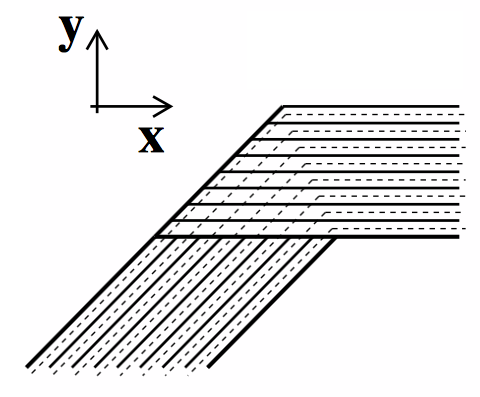
\includegraphics[width=0.4\textwidth]{LCDetectorsAndPFlow/Plots/Pictures/PseudoLayer1.png}}
\hspace{1cm}
\subfloat[]{\label{fig:pseudolayer2}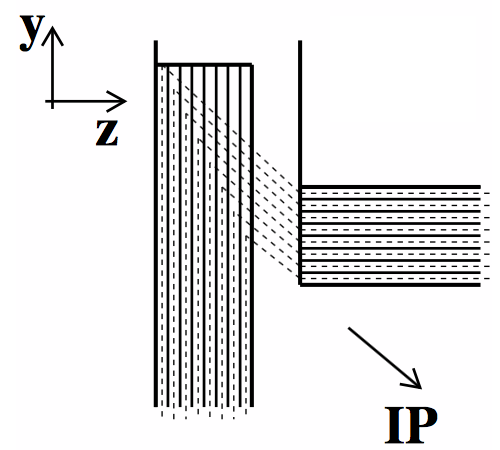
\includegraphics[width=0.4\textwidth]{LCDetectorsAndPFlow/Plots/Pictures/PseudoLayer2.png}}
\caption[Schematic showing the definition of the pseudo-layer assignment for calorimeter hits.  The solid lines indicate the positions of the physics ECal layers and the dashed lines show the definition of the virtual pseudo-layers.  \protect\subref{fig:pseudolayer1} The $xy$-view showing the ILD ECal stave structure.  \protect\subref{fig:pseudolayer2} The $xz$ view showing a possible layout for the ECal barrel/endcap overlap region.  The pseudo-layers are defined using projection back to the IP.  Figures taken from \cite{arXiv:0907.3577}.]{Schematic showing the definition of the pseudo-layer assignment for calorimeter hits.  The solid lines indicate the positions of the physics ECal layers and the dashed lines show the definition of the virtual pseudo-layers.  \protect\subref{fig:pseudolayer1} The $xy$-view showing the ILD ECal stave structure.  \protect\subref{fig:pseudolayer2} The $xz$ view showing a possible layout for the ECal barrel/endcap overlap region.  The pseudo-layers are defined using projection back to the IP.  Figures taken from \cite{arXiv:0907.3577}.}
\label{fig:pseudolayer}
\end{figure} 

\begin{figure}[h!]
\centering
\subfloat[]{\label{fig:association1}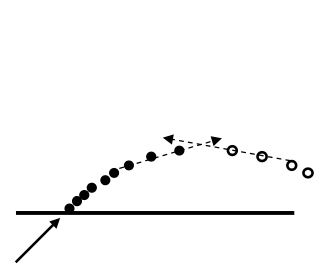
\includegraphics[width=0.2\textwidth]{LCDetectorsAndPFlow/Plots/Pictures/Association1.png}}
\hspace{5mm}
\subfloat[]{\label{fig:association2}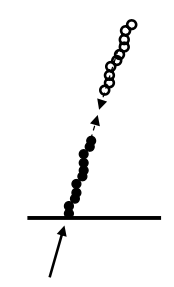
\includegraphics[width=0.2\textwidth]{LCDetectorsAndPFlow/Plots/Pictures/Association2.png}}
\hspace{5mm}
\subfloat[]{\label{fig:association3}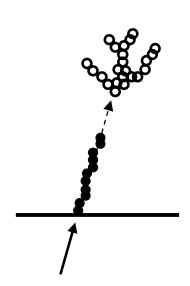
\includegraphics[width=0.2\textwidth]{LCDetectorsAndPFlow/Plots/Pictures/Association3.png}}
\hspace{5mm}
\subfloat[]{\label{fig:association4}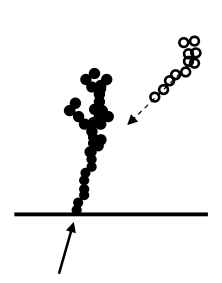
\includegraphics[width=0.2\textwidth]{LCDetectorsAndPFlow/Plots/Pictures/Association4.png}} \\
\subfloat[]{\label{fig:association5}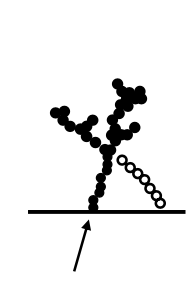
\includegraphics[width=0.2\textwidth]{LCDetectorsAndPFlow/Plots/Pictures/Association5.png}}
\hspace{5mm}
\subfloat[]{\label{fig:association6}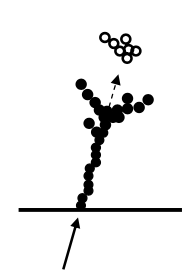
\includegraphics[width=0.2\textwidth]{LCDetectorsAndPFlow/Plots/Pictures/Association6.png}}
\hspace{5mm}
\subfloat[]{\label{fig:association7}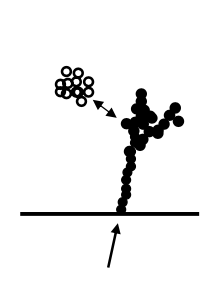
\includegraphics[width=0.2\textwidth]{LCDetectorsAndPFlow/Plots/Pictures/Association7.png}}
\hspace{5mm}
\subfloat[]{\label{fig:association8}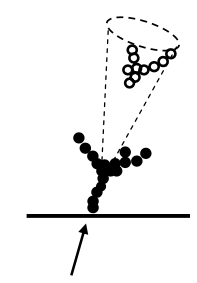
\includegraphics[width=0.2\textwidth]{LCDetectorsAndPFlow/Plots/Pictures/Association8.png}}
\hspace{5mm}
\subfloat[]{\label{fig:association9}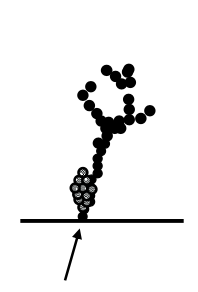
\includegraphics[width=0.2\textwidth]{LCDetectorsAndPFlow/Plots/Pictures/Association9.png}}
\caption[The main topological rules for cluster merging: \protect\subref{fig:association1} looping track segments; \protect\subref{fig:association2} track segments with gaps; \protect\subref{fig:association3} track segments pointing to hadronic showers; \protect\subref{fig:association4} track-like neutral clusters pointing back to a hadronic shower; \protect\subref{fig:association5} back-scattered tracks from hadronic showers; \protect\subref{fig:association6} neutral clusters which are close to a charged cluster; \protect\subref{fig:association7} a neutral cluster near a charged cluster; \protect\subref{fig:association8} cone association; and \protect\subref{fig:association9} recover of photons which overlap with a track segment.  In each case the arrow indicates the track, the filled points represent the hits in the associated cluster and the open points represent hits in the neutral cluster.  Figures taken from \cite{arXiv:0907.3577}.]{The main topological rules for cluster merging: \protect\subref{fig:association1} looping track segments; \protect\subref{fig:association2} track segments with gaps; \protect\subref{fig:association3} track segments pointing to hadronic showers; \protect\subref{fig:association4} track-like neutral clusters pointing back to a hadronic shower; \protect\subref{fig:association5} back-scattered tracks from hadronic showers; \protect\subref{fig:association6} neutral clusters which are close to a charged cluster; \protect\subref{fig:association7} a neutral cluster near a charged cluster; \protect\subref{fig:association8} cone association; and \protect\subref{fig:association9} recover of photons which overlap with a track segment.  In each case the arrow indicates the track, the filled points represent the hits in the associated cluster and the open points represent hits in the neutral cluster.  Figures taken from \cite{arXiv:0907.3577}.}
\label{fig:associations}
\end{figure} 

The application of the pattern recognition algorithms in PandoraPFA when combined with a highly segmented detector make particle flow calorimetry a reality.  In turn this provides excellent jet energy resolution for studying many interesting physics processes at the linear collider experiment.

%======================================================================================== 
%======================================================================================== 

\section{Performance}
\label{sec:performance}
The fundamental principle of particle flow calorimetry is to measure the energy of a particle passing through a detector in whichever sub-detector offers the best energy resolution.  For particle collider experiments, this involves measuring the momenta of charged particles using the curvature of the track they create in the detector.  This offers extremely good energy resolution in comparison to the traditional calorimetric approach.  

As many physics processes of interest at the linear collider involve multi-jet final states \cite{Abramowicz:2016zbo}, good jet energy resolution is a crucial aspect of detector performance.  As shown in chapter \ref{chap:PhysicsAnalysis}, the sensitivity of the linear collider experiment to areas of new physics can determined using reconstructed jet energies.  Furthermore, parameters derived from the energy measurements of jets are extremely useful for identification of physics channels of interest.  Therefore, a key metric for describing detector performance is the jet energy resolution.  Jet energy resolution in particular can benefit from the application of particle flow calorimetry as $\approx 70 \%$ of the energy of jets are carried in the form of charged particles.  As particle flow aims to measure the energy of charged particles using the tracker, it has the potential to offer extremely large benefits when measuring jet energies in comparison to the traditional calorimetric approach.  

%========================================================================================

\subsection{Jet Energy Resolution}
The jet energy resolution in these studies was determined through the simulation of off mass shell Z boson events decaying to light quarks (u, d, s).  PYTHIA version 6.4 \cite{Sjostrand:2006za}, which had been trained on fragmentation data from the OPAL experiment \cite{Alexander:1995bk}, was used to generate these events.  The decay of tau leptons appearing in the day was simulated using TAUOLA \cite{Was:2000st}.  Detector simulation and event reconstruction was carried out as described in sections \ref{sec:simulation} and \ref{sec:reconstruction} respectively.  

As the Z boson in these events is produced at rest, the typical decays form two mono-energetic jets that are produced back-to-back as shown in figure \ref{fig:500GeVzudsevtdisplay}.  Only events where $|\text{cos}(\theta)| < 0.7$, where $\theta$ is the polar angle of the quarks, are used in the jet energy resolution calculation.  This ensures little energy is lost down the beam axis.  Using these events, the jet energy resolution was calculated as follows: 
\begin{equation} 
\frac{\text{RMS}_{90}(E_{j})}{\text{Mean}_{90}(E_{j})} = \frac{\text{RMS}_{90}(E_{jj})}{\text{Mean}_{90}(E_{jj})} \times \sqrt{2} \text{ ,}
\end{equation}
\noindent where $E_{jj}$ is the total reconstructed energy.  The variables $\text{Mean}_{90}(E_{jj})$ and $\text{RMS}_{90}(E_{jj})$ are the mean and root mean squared (RMS) of the $E_{jj}$ distribution respectively.  They are calculated across the range of $E_{jj}$ with the smallest RMS containing at least 90\% of the data.  This definition is used to remove the effect of outliers in the distribution \cite{arXiv:0907.3577}.  If all associations between charged particle tracks and calorimeter clusters were correctly made, the reconstructed jet energy distribution would be Gaussian.  However, the effect of confusion on certain events will distort this distribution and broaden the tails significantly.  If the full range were to be used in the jet energy resolution calculation, the effect of these tails is overinflated.  If the distribution of reconstructed jet energies is truncated to the narrowest range of the data containing at least $90\%$ of the data, the effect of these tails can be negated.  This removes events where confusion is dominant, which makes the jet energy resolution metric far more robust and representative of the bulk of the data.  

\begin{figure}[h!]
\centering
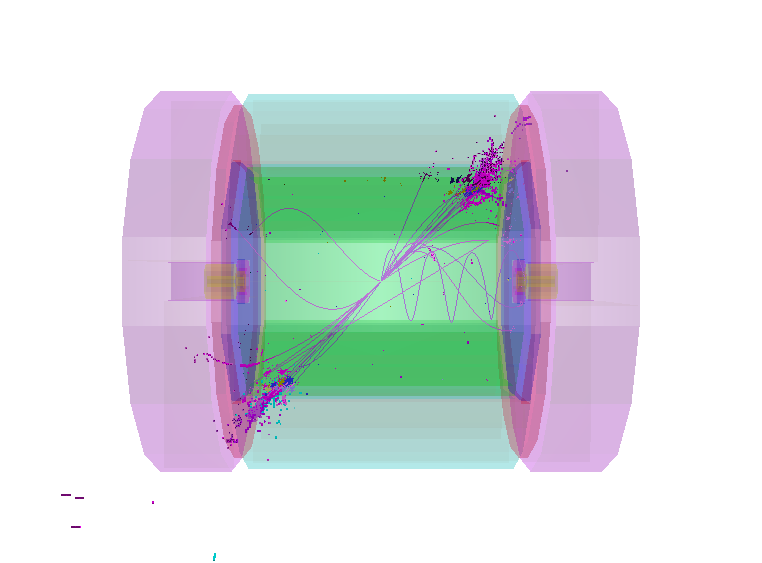
\includegraphics[width=0.75\textwidth]{OptimisationStudies/Plots/MethodDescription/500GeVEvent.png}
\caption[500~GeV di-jet Z$\rightarrow$uds event display for nominal ILD detector.]{500~GeV di-jet Z$\rightarrow$uds event display for nominal ILD detector.}
\label{fig:500GeVzudsevtdisplay}
\end{figure} 

\begin{figure}[h!]
\centering
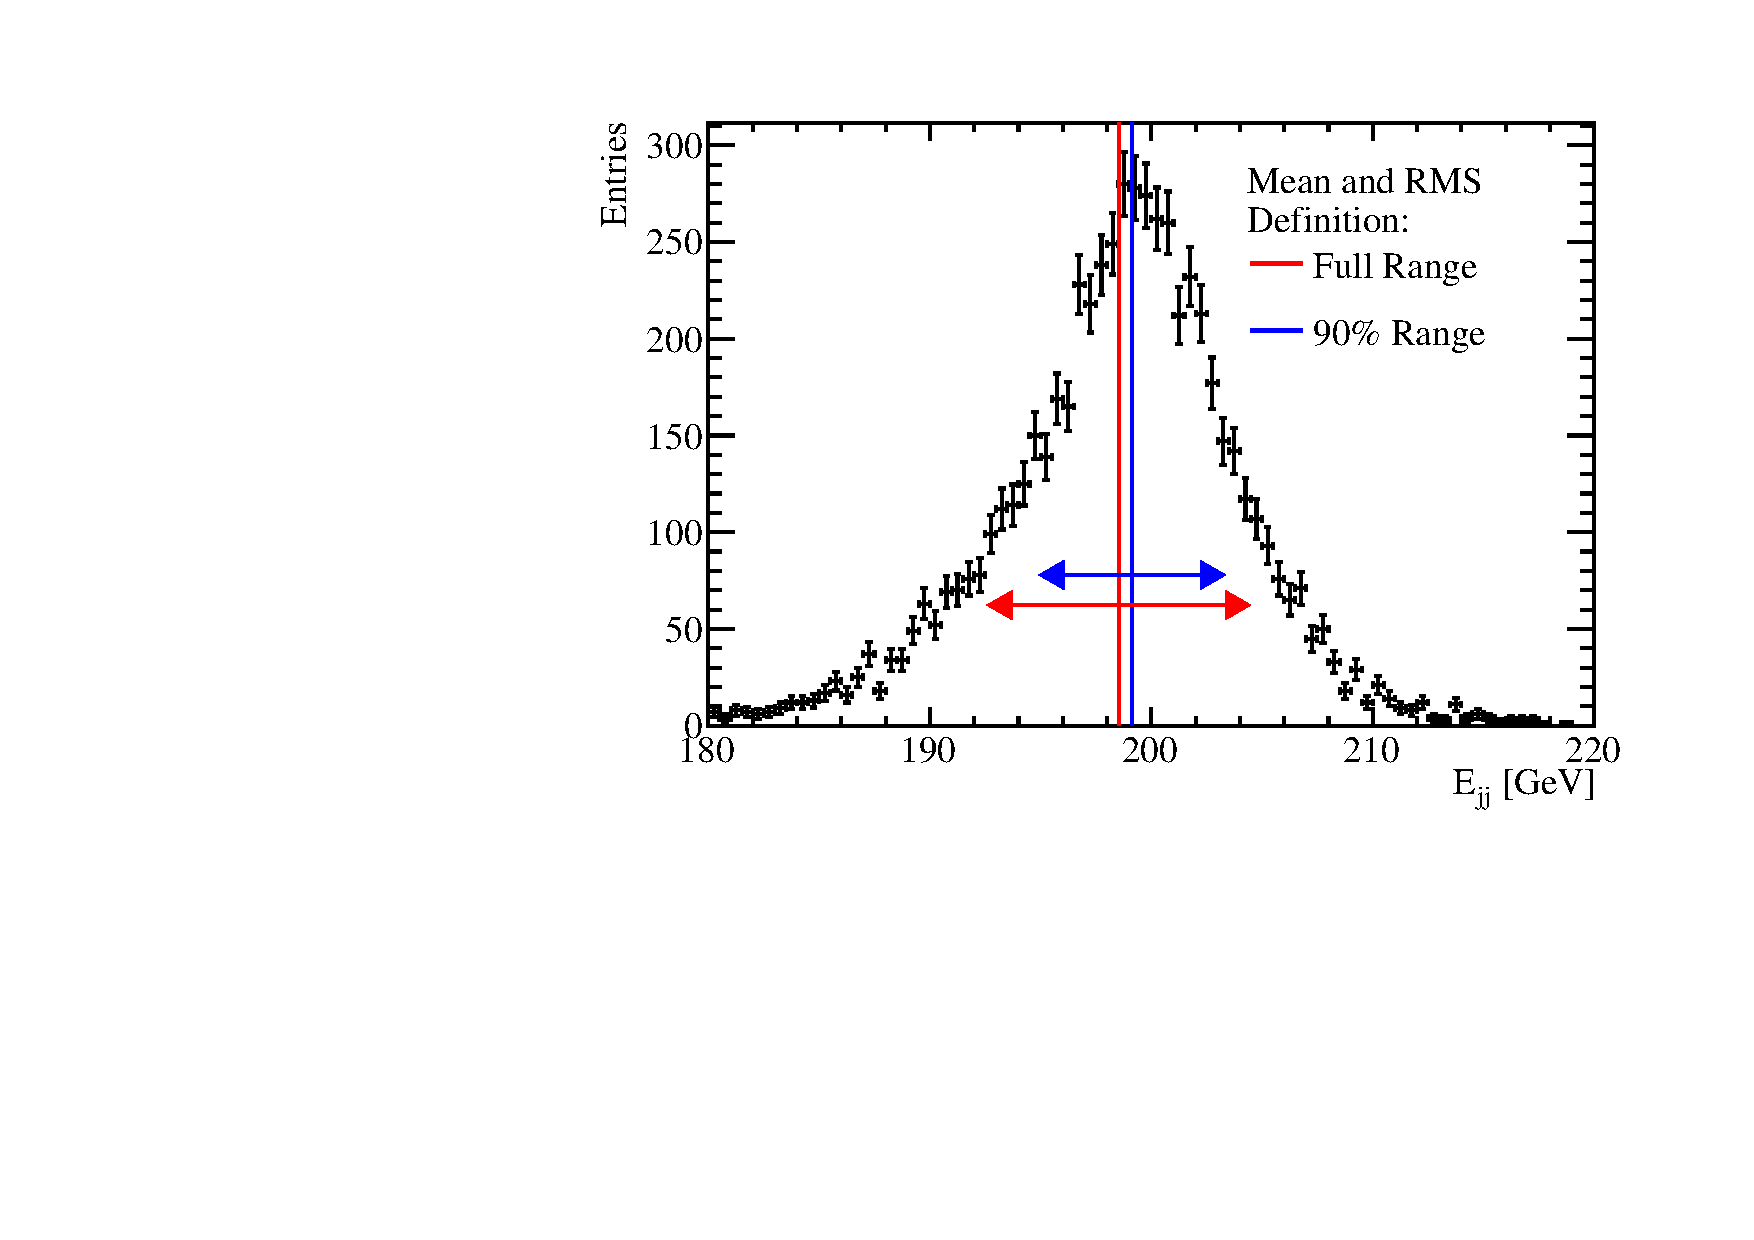
\includegraphics[width=0.5\textwidth]{OptimisationStudies/Plots/MethodDescription/RMS90Plot.pdf}
\caption[Definition of jet energy resolution.   Reconstructed jet energy for 200~GeV di-jet Z$\rightarrow$uds events for nominal ILD detector.  The solid vertical line shows the mean of the distribution and the horizontal arrows indicate the mean $\pm$ the root mean square (RMS) of the distribution.  The red and blue lines represent the mean and RMS calculated using the full range and 90\% of the full range with the smallest RMS.]{Definition of jet energy resolution.   Reconstructed jet energy for 200~GeV di-jet Z$\rightarrow$uds events for nominal ILD detector.  The solid vertical line shows the mean of the distribution and the horizontal arrows indicate the mean $\pm$ the root mean square (RMS) of the distribution.  The red and blue lines show the mean and RMS calculated using the full range and 90\% of the full range with the smallest RMS respectively.}
\label{fig:rms90defintion}
\end{figure} 

An example of the application of this metric can be found in figure \ref{fig:rms90defintion}.  In this example $\text{RMS}(E_{j})$, the RMS calculated using the full range, is 5.8~GeV, while $\text{RMS}_{90}(E_{j})$, the RMS using the reduced range, is 4.1~GeV.  This corresponds to a reduction in the jet energy resolution from $4.1\%$ to $2.9\%$, which clearly shows an overemphasis of the tails of the distribution when using the full jet energy range.

In the subsequent analysis a range of di-jet energies were considered ranging from the Z mass, 91~GeV, to the nominal running energy of the ILC, 500~GeV.  Each event sample contained 10,000 events generated isotropically so that, given the polar angle cut, approximately 7,000 events contribute to the jet energy resolution calculation. 

%========================================================================================

\subsection{Decomposition of the Jet Energy Resolution}
\label{sec:jerdecomposition}
It is possible to gain additional insight into the detector performance by cheating the pattern recognition, the clustering of calorimeter hits together and the creation of track to cluster associations, using MC information.  Cheating the pattern recognition removes the effect of confusion as it ensures no errors are made when either clustering calorimeter hits together or when associating charged particle tracks to those calorimeter clusters.  This allows the detector performance to be deconstructed into two terms; one related exclusively to the intrinsic energy resolution of the detector and another related to the pattern recognition confusion.  The additional information this provides is extremely useful for characterising changes to the overall detector performance.  

The intrinsic energy resolution contribution to the jet energy resolution is determined by fully cheating the pattern recognition; in this case all confusion is negated.  The total confusion is defined as the quadrature difference between the jet energy resolution using the standard reconstruction and this fully cheated reconstruction.  Furthermore, it is possible to cheat the pattern recognition associated with individual types of particles.  This is particularly useful for studies related to the ECal as, by cheating the photon pattern recognition, it is possible to isolate the confusion associated with photons.  The photon confusion is defined as the quadrature difference between the jet energy resolution using the standard reconstruction and the reconstruction where the photon pattern recognition is cheated.  Examples of the calculation of the various confusion terms defined above are given in table \ref{table:confusioncalculation}.

\begin{table}[h!]
\centering
\begin{tabular}{ l r}
\hline
Reconstruction & Jet Energy Resolution [\%] \\
\hline
Standard Reconstruction (No MC Information) & $a = 2.97\pm0.05$ \\
Cheating Entire Reconstruction & $b = 1.69\pm0.02$ \\
Confusion & $\sqrt{a^{2}-b^{2}} = 2.45\pm0.05$ \\
\hline
Cheating Photon Reconstruction & $c = 2.73\pm0.04$ \\
Photon Confusion & $\sqrt{a^{2}-c^{2}} =1.18\pm0.06$ \\
\hline
\end{tabular}
\caption[Example calculation of the confusion contributions to the jet energy resolution.  These jet energy resolutions are for 250~GeV jets using the nominal ILD detector model and are calculated using the range of jet energies with the smallest RMS containing at least 90\% of the data.]{Example calculation of the confusion contributions to the jet energy resolution.  These jet energy resolutions are for 250~GeV jets using the nominal ILD detector model and are calculated using the range of jet energies with the smallest RMS containing at least 90\% of the data.}
\label{table:confusioncalculation}
\end{table}

A common feature that is observed in these calibration studies is that as the intrinsic energy resolution of a calorimeter improves, the effect of confusion is reduced.  This occurs as a better energy resolution means more precise comparisons can be made between the energy of a cluster of calorimeter hits and the momentum of any charged particle tracks associated to it.  Comparisons such as these are made by PandoraPFA to determine whether the track cluster associations that have been made are consistent.  If a large discrepancy is observed between the cluster energy and track momenta, the clustering of calorimeter hits is modified until a consistent association can be made.  For more details on this comparison see chapter \ref{chap:pflowandlcdetectors}.  This consistency check vastly reduces the number of errors made when clustering calorimeter hits and associating charged particle tracks to those clusters i.e. the confusion.  Therefore, improving the precision of this consistency check, by improving the energy resolution, reduces the effect of confusion.  

%========================================================================================

\subsection{Single Particle Energy Resolution}
The energy resolution for individual particles is crucial for a number of physics studies of interest to the linear collider, such as $\gamma$ energy resolutions in the study of anomalous triple and quartic gauge couplings \cite{Chatrchyan:2013fya,ATLAS:2012mec,Chatrchyan:2014bza}.  Therefore, $\gamma$ and $K^{0}_{L}$ energy resolutions, alongside the jet energy resolution, will be considered in these optimisation studies.  As both $\gamma$ and $K^{0}_{L}$ are uncharged, their energy measurements will be made using the calorimeters as opposed to the tracker.  $\gamma$s are a natural choice of particle to consider as they are particularly relevant for several physics studies and, as they are largely contained within the ECal, they will be highly sensitive to changes in the ECal performance.  $K^{0}_{L}$s were used as, analogously to $\gamma$s and the ECal, their energies are primarily measured using the HCal.  In general, neutral hadron energy resolutions are less crucial to physics studies, however, they do make crucial contribution to the jet energy resolution that should not be overlooked.  The reported $\gamma$ energy resolutions were determined using events containing a single 100~GeV $\gamma$, while the $K^{0}_{L}$ energy resolutions were determined using events containing a single 50~GeV $K^{0}_{L}$.  These energies were chosen to be as large as possible, to maximise sampling of the calorimeter response, while minimising the affect of leakage of energy from the ECal to the HCal for the $\gamma$ events and leakage of energy out of the rear of the HCal for the $K^{0}_{L}$ events.

The energy resolution for these single particle samples is determined using a Gaussian fit to the reconstructed energy distributions.  To aid convergence, the fit was applied to the narrowest range of the reconstructed energy distribution containing at least 75\% of the data.  The single particle energy resolution is defined as the standard deviation divided by the mean of the fitted Gaussian.  For each energy resolution calculation, a total of 10,000 events were used to populate the reconstructed energy distribution.  For clarity, a cut of $|\text{cos}(\theta)| < 0.7$ was applied to veto events where particles travelled down the beam pipe or where they passed through the barrel/endcap overlap region.  An example of the reconstructed energy distributions for 100~GeV $\gamma$s and 50~GeV $K^{0}_{L}$s, alongside the Gaussian fits used to determine the energy resolutions, are shown in figure \ref{fig:singleparticleenergyhists}.  The errors quoted on single particle energy resolutions are determined by propagating the errors reported from the Gaussian fit into the resolution calculation.  

\begin{figure}[h!]
\centering
\subfloat[]{\label{fig:kaonsingleparticleenergyhist}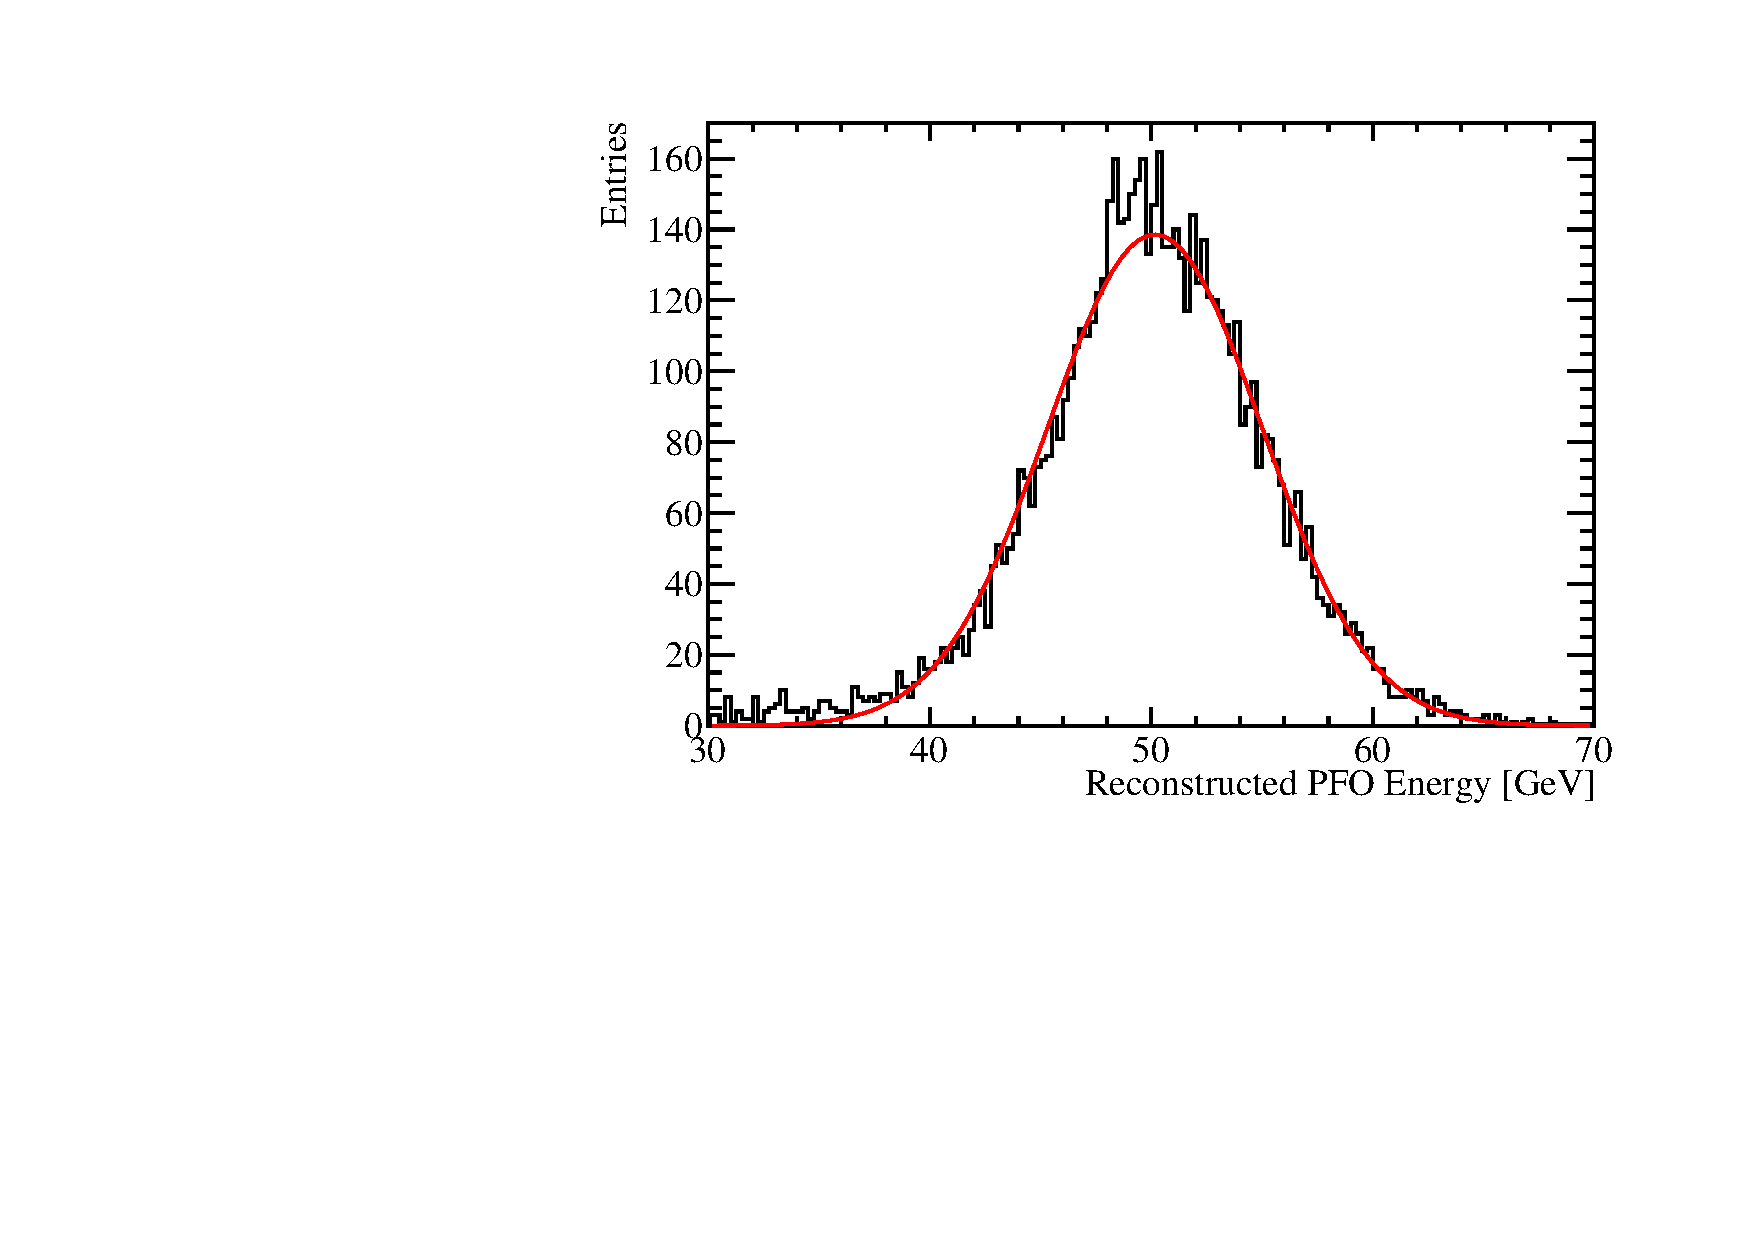
\includegraphics[width=0.5\textwidth]{OptimisationStudies/Plots/EnergyResolution/EKaon0L_50GeV.pdf}}
\subfloat[]{\label{fig:photonsingleparticleenergyhist}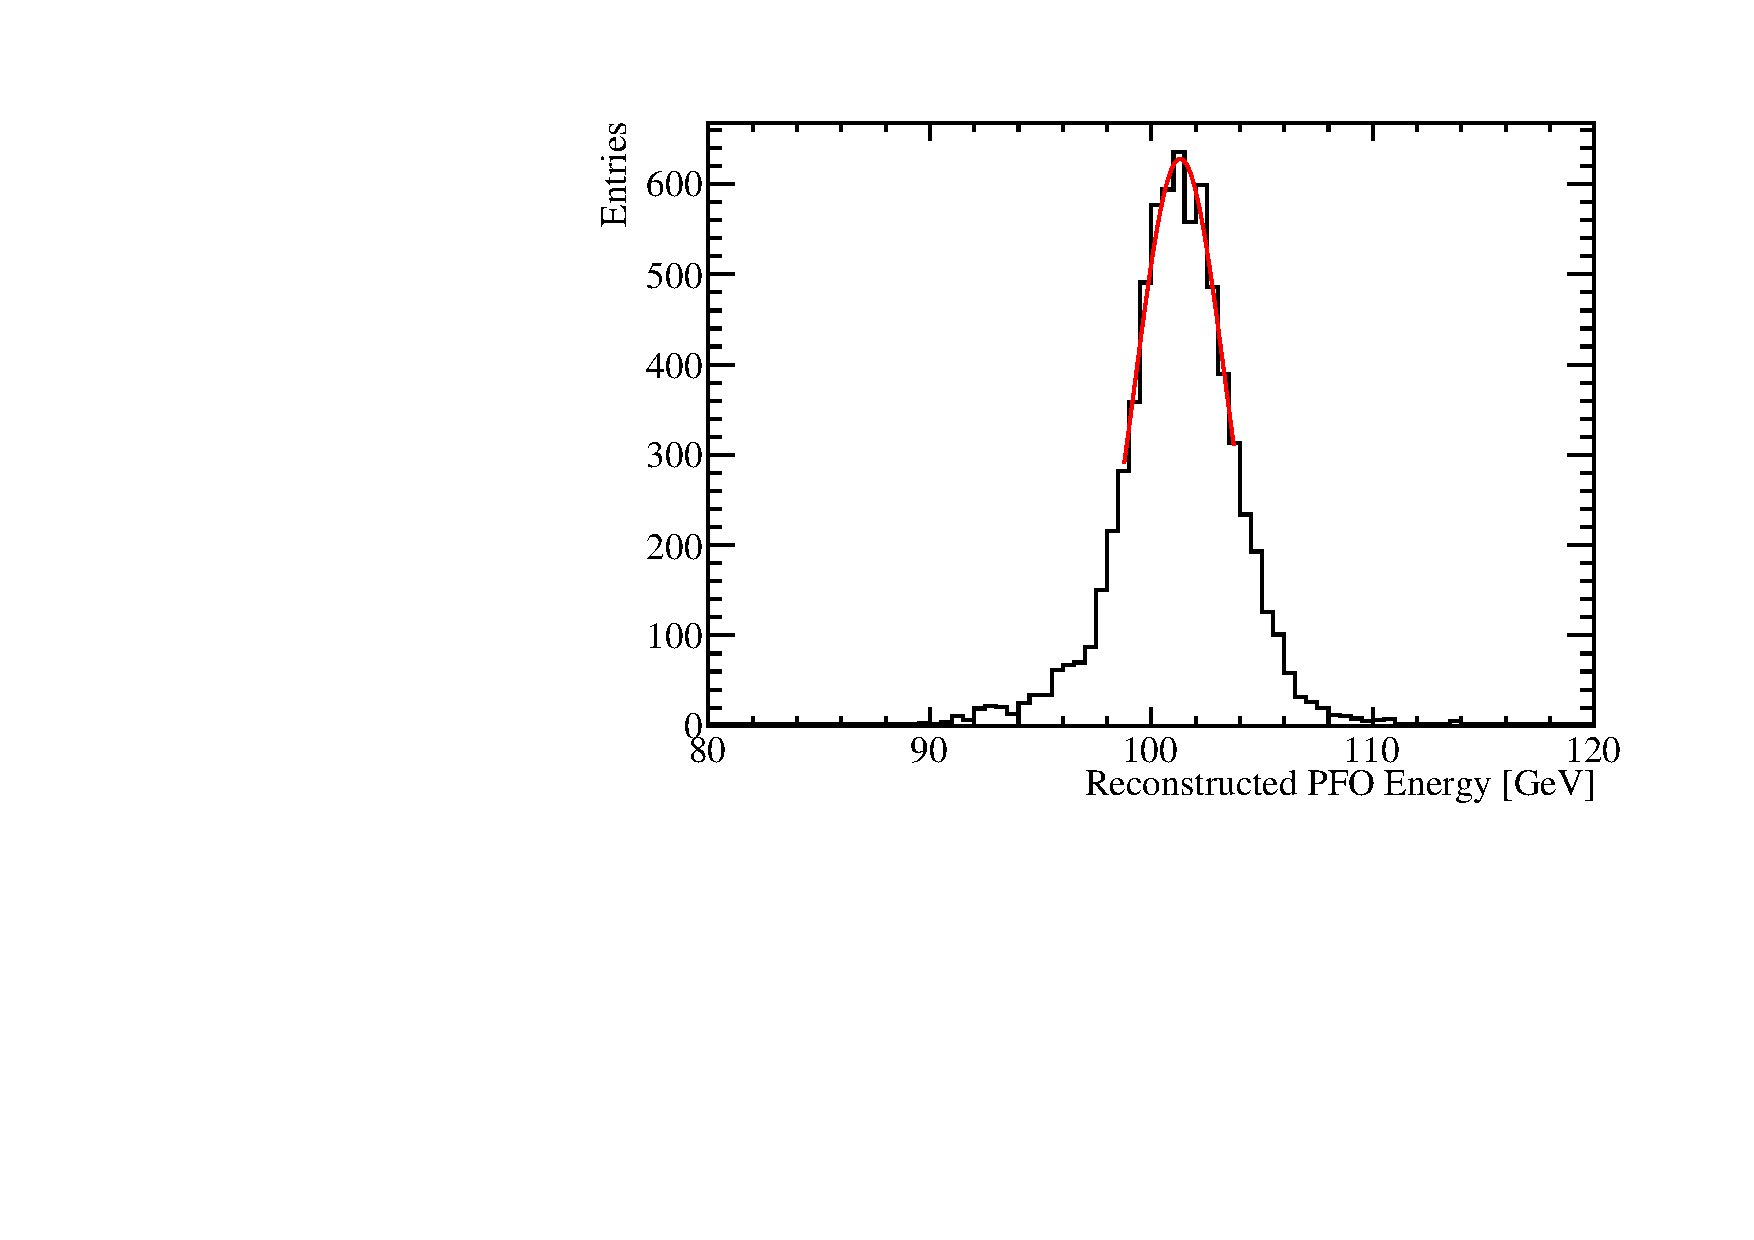
\includegraphics[width=0.5\textwidth]{OptimisationStudies/Plots/EnergyResolution/EPhoton_100GeV.pdf}}
\caption[The reconstructed energy distribution for \protect\subref{fig:kaonsingleparticleenergyhist} 50~GeV $K^{0}_{L}$ and \protect\subref{fig:photonsingleparticleenergyhist} 100~GeV $\gamma$ events.  The red line shows a Gaussian fit used to parameterise the detector performance.  The fit was applied to the truncated range of the reconstructed PFO energy distribution containing at least 75\% of the data with the narrowest RMS.  The nominal ILD model was used in this simulation.]{The reconstructed energy distribution for \protect\subref{fig:kaonsingleparticleenergyhist} 50~GeV $K^{0}_{L}$ and \protect\subref{fig:photonsingleparticleenergyhist} 100~GeV $\gamma$ events.  The red line shows a Gaussian fit used to parameterise the detector performance.  The fit was applied to the truncated range of the reconstructed PFO energy distribution containing at least 75\% of the data with the narrowest RMS.  The nominal ILD model was used in this simulation.}
\label{fig:singleparticleenergyhists}
\end{figure}

%========================================================================================
%========================================================================================

\section{Summary of ILD Detector Performance}
\label{sec:nominaldetectorperformance}
The following section outlines the nominal ILD detector performance using the metrics outlined in section \ref{sec:performance}.  

The reconstructed energy distributions for particles whose energies are measured using calorimeters will be Gaussian.  This is the case for sampling calorimeters as the active material in each calorimeter hit essentially counts the number of charged particle tracks passing through it, or possible the number of photons for scintillator options.  An estimation of the total energy deposited in a calorimeter hit, including the absorber material, can be made based upon this number of tracks or photons.  For more details on how this estimation is made see chapter \ref{chap:energyestimators}.  Finally, the energy of the entire particle shower is estimated by grouping together calorimeter hits and summing their energy.  As each calorimeter hit energy is an independent random measurement the particle shower energy will, by the central limit theorem, have a Gaussian distribution.  

As each calorimeter hit involves counting a number of objects, charged particle tracks or photons, Poisson statistics governing the distribution of calorimeter hit energies.  If the mean of the distribution of the energy of a cluster of calorimeter hits is $\lambda = N$, where $N$ is the mean number of objects the are measured in the calorimeters, the standard deviation of that distribution is $\sigma = \sqrt{\lambda} = \sqrt{N}$ and the energy resolution is $\frac{\sigma}{\lambda} = \frac{1}{\sqrt{N}}$.  As the total shower energy, $E_{Reco}$, is proportional to $N$ the energy resolution for a particle shower in an ideal calorimeter is $\frac{\sigma_{Reco}}{E_{Reco}} = \frac{a}{\sqrt{E_{Reco}}}$.  In reality, it is typical to express the energy resolution of a calorimeter in the following form
%
\begin{equation} 
\frac{\sigma_{Reco}}{E_{Reco}} = \frac{a}{\sqrt{E_{Reco}}} \oplus b \oplus \frac{c}{E_{Reco}}\text{ ,}
\end{equation}
%
\noindent where the $b$ term is a constant term that accounts for a variety of instrumental effects that do not depend on energy, e.g. mechanical imperfections, and the $c$ term accounts for electrical noise \cite{Fabjan:2003aq}.  Here $\oplus$ denotes the quadrature sum of variables.  

Prototypes of the various ILD calorimeter options have been constructed and validated using test beam measurements.  The energy resolution of the ILD ECal, determined from test beam measurements, was parameterised as $\frac{16.6}{\sqrt{E_{Reco}}} \oplus 1.1 \%$ for the silicon option and $\frac{12.9}{\sqrt{E_{Reco}}} \oplus 1.2 \%$ for the scintillator option \cite{Behnke:2013lya}.  The electrical noise was deemed sufficiently small that the $c$ term in the parameterisation could be neglected in both cases.  These results were determined using an $\text{e}^{-}$ test beam with energies ranging up to $\approx 40$~GeV.  This parametrisation is compared to the full ILD detector simulation in figures \ref{fig:ecalsinominalres} and \ref{fig:ecalscnominalres} for the silicon and scintillator ECal options respectively.  The test beam parameterisation of the energy resolution for the silicon ECal option is almost identical to the energy resolution observed in the full simulation.  At very high energies, $\approx 500$~GeV, the ECal is no longer sufficient to fully contain the $\gamma$s and so leakage of energy into the HCal leads to a minor degradation in the simulated energy resolution.  This accounts for the worse energy resolution seen in the full simulation when compared to an extrapolation of the test beam parameterisation at high energies.  The test beam parameterisation of the energy resolution for the scintillator ECal option is significantly better than that observed in the full simulation, which is most likely due to an imperfect implementation of the scintillator ECal within the full detector simulation.  The $\gamma$ energy resolutions seen in the full ILD simulation are similar for the silicon and scintillator ECal options.      

Similarly, the energy resolution, determined from test beam measurements, for the nominal ILD HCal was parameterised as $\frac{57.6}{\sqrt{E_{Reco}}} \oplus 1.6 \%$ \cite{Adloff:2012gv}.  A comparison between this test beam parameterisation and the full ILD simulation, using the silicon ECal option, is shown in figure \ref{fig:hcalnominalres}.  The test beam measurements were made using $\pi^{\pm}$s with energies ranging from 10 to 80~GeV, while the full ILD simulation used $K^{0}_{L}$s ranging from 10 to 100~GeV.  The deviation between the test beam parameterisation and the full ILD simulation, which grows at as the $K^{0}_{L}$ energy increases, is most likely due to the treatment of energy deposits leaking out of the back of the HCal.  In the test beam studies, to minimise the effect of leakage, events were only considered if the particle showers started developing at the front of the HCal.  In the full simulation studies, all particle showers were used, which means some energy will have leaked out of the back of the calorimeters and been deposited in the uninstrumented solenoid region of the detector resulting in a degradation in the energy resolution.   

Figure \ref{fig:jernominalres} shows the jet energy resolution as a function of jet energy for the full ILD simulation.  Alongside this, the intrinsic energy resolution and confusion contributions to the jet energy resolution are also presented.  The jet energy resolution at low energies is dominated by the intrinsic energy resolution of the detector, while at high energies it is dominated by the effect of confusion.  This is to be expected because the intrinsic energy resolution of the calorimeters is proportional $~\frac{1}{\sqrt{E_{j}}}$.  On the other hand, confusion grows with energy because increasing energy leads to more dense event topologies, which makes pattern recognition more challenging.  The total jet energy resolution for the ILD detector are sufficiently small, $\frac{\sigma_{E_{j}}}{E_{j}} \lesssim 3.8\%$ \cite{Behnke:2013lya, arXiv:0907.3577, Linssen:2012hp}, across the energy range considered to make separation of the hadronic decays of the W and Z bosons possible, which is one of the key requirements for the future linear collider.

\begin{figure}[h!]
\centering
\subfloat[]{\label{fig:ecalsinominalres}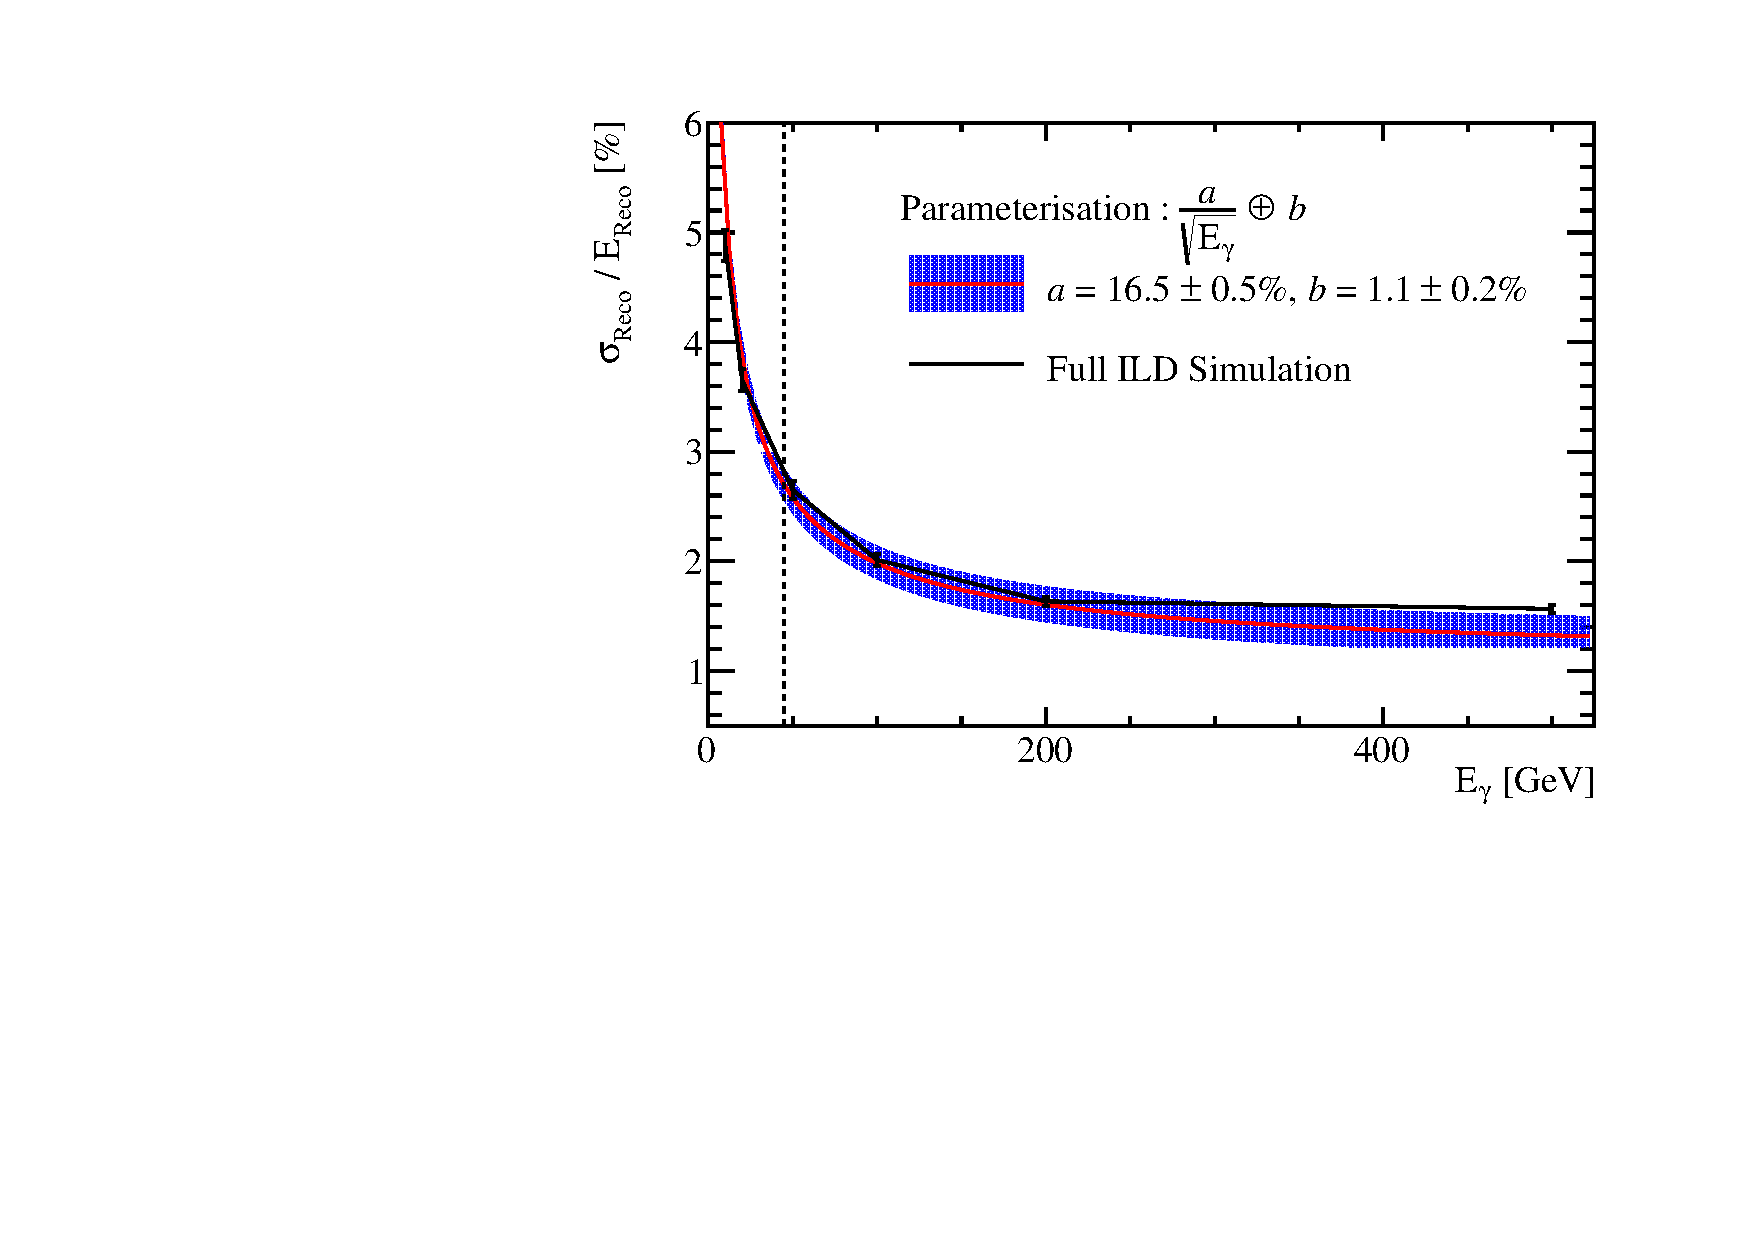
\includegraphics[width=0.5\textwidth]{OptimisationStudies/Plots/EnergyResolution/ER_vs_EGamma_SiECal.pdf}}
\subfloat[]{\label{fig:ecalscnominalres}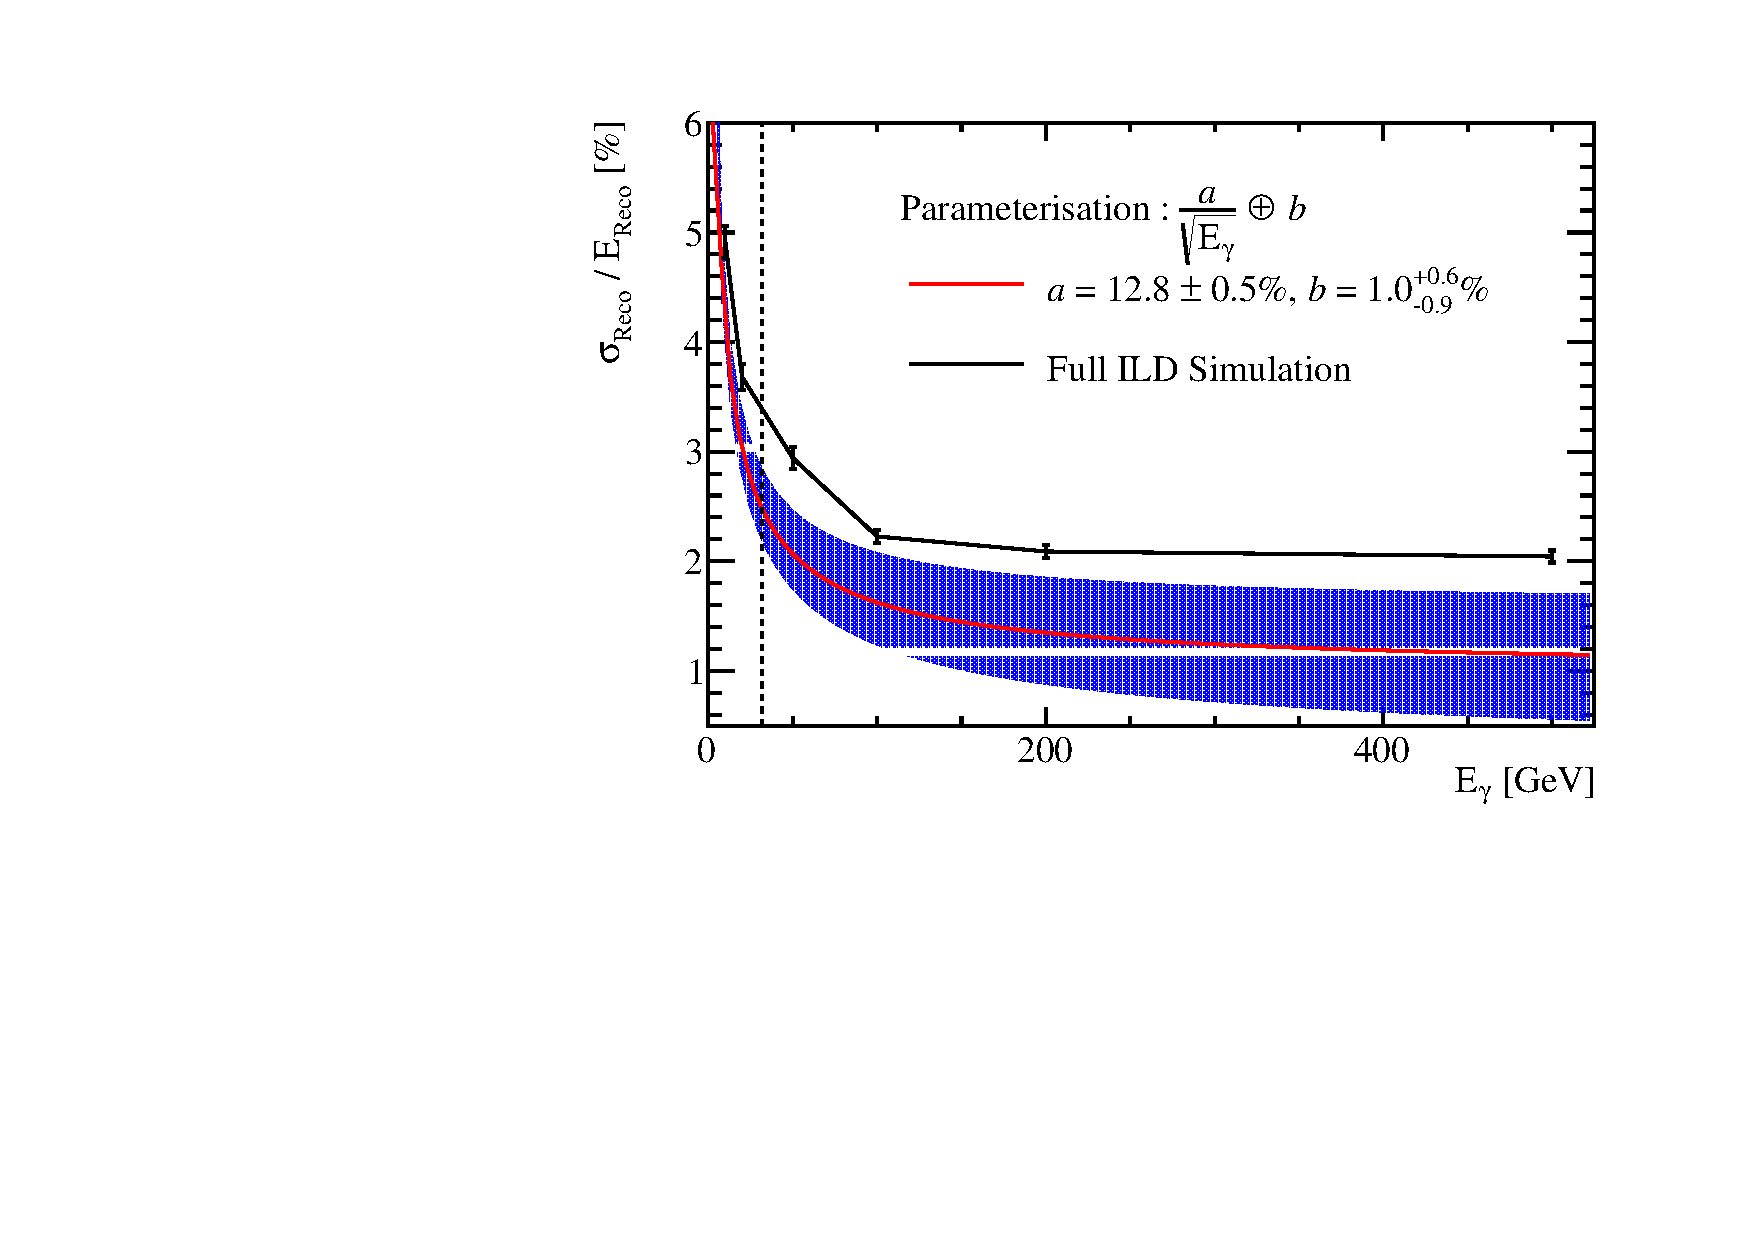
\includegraphics[width=0.5\textwidth]{OptimisationStudies/Plots/EnergyResolution/ER_vs_EGamma_ScECal.pdf}}\\
\subfloat[]{\label{fig:hcalnominalres}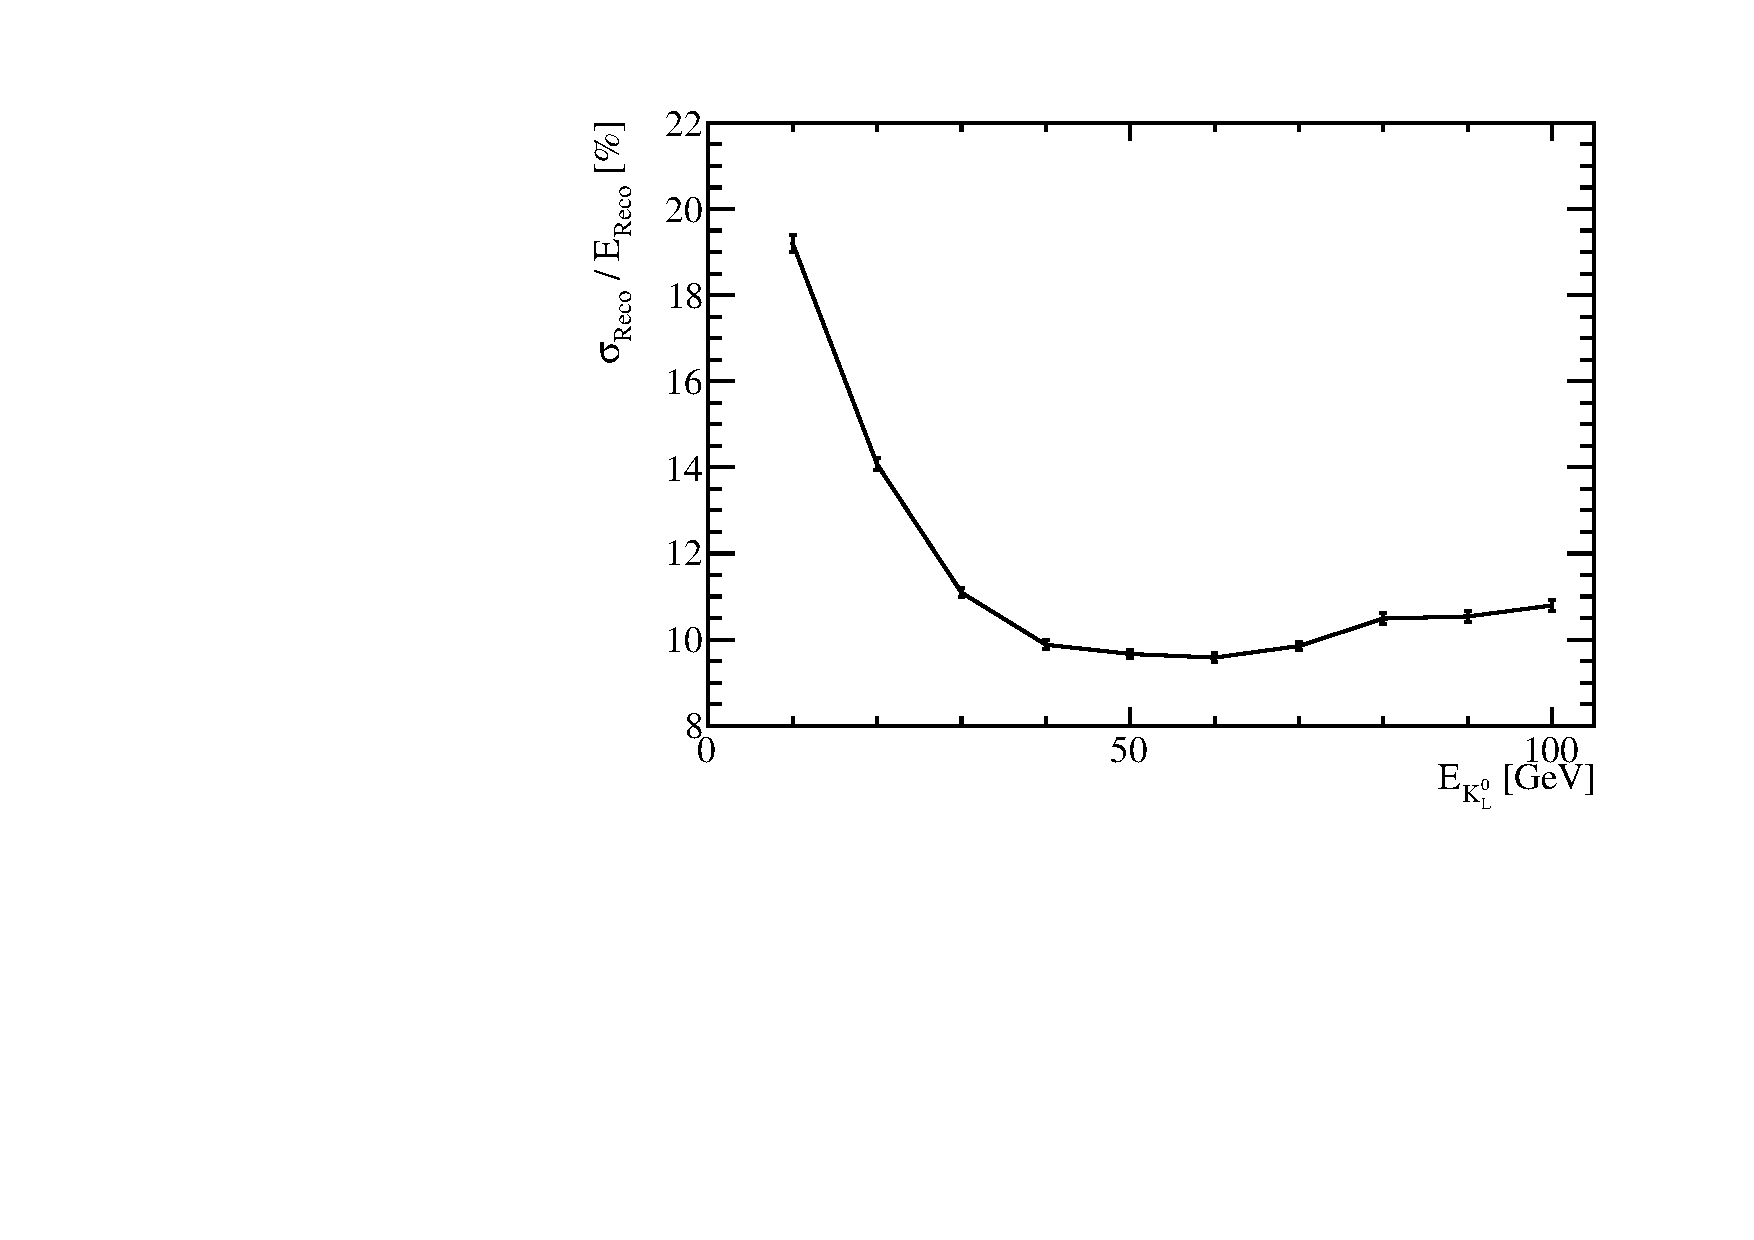
\includegraphics[width=0.5\textwidth]{OptimisationStudies/Plots/EnergyResolution/ER_vs_EKaon0L_SiECal.pdf}}
\subfloat[]{\label{fig:jernominalres}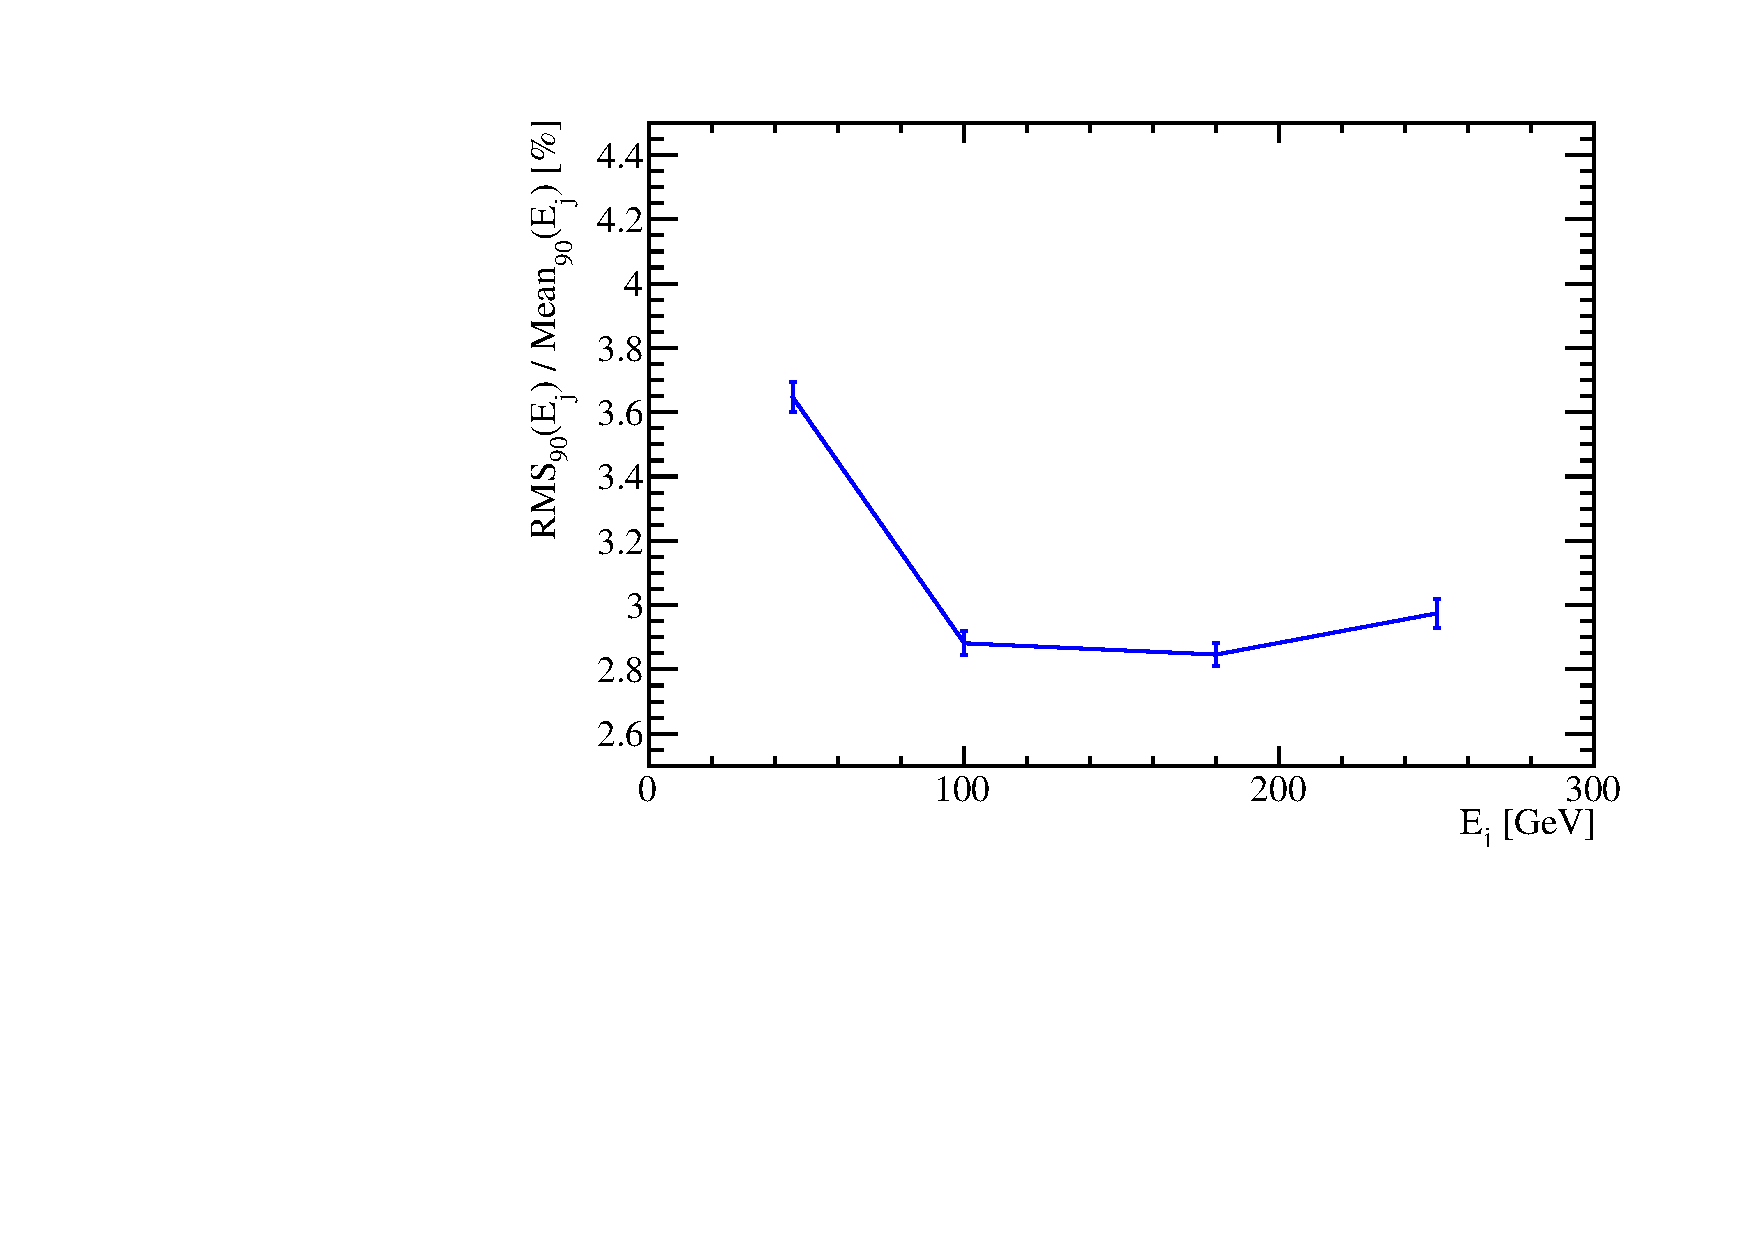
\includegraphics[width=0.5\textwidth]{OptimisationStudies/Plots/JetEnergyResolutions/JER_vs_JetEnergy_NominalDetectorPerformance.pdf}}
\caption[\protect\subref{fig:ecalsinominalres} The energy resolution as a function of $\gamma$ energy for the silicon ECal option.  The black markers indicate the energy resolutions for the full ILD simulation and the red dotted line shows the test beam parameterisation of the ECal energy resolution.  \protect\subref{fig:ecalscnominalres} The energy resolution as a function of $\gamma$ energy for the scintillator ECal option.  The black markers indicate the energy resolutions for the full ILD simulation and the red dotted line shows the test beam parameterisation of the ECal energy resolution.  \protect\subref{fig:hcalnominalres} The energy resolution as a function of neutral hadron energy.  The black markers indicate the energy resolutions for the full ILD simulation, with the silicon ECal option, which was determined using $K^{0}_{L}$s.  The red dotted line shows the test beam parameterisation of the HCal energy resolution, which was determined using $\pi^{\pm}$s.  \protect\subref{fig:jernominalres} The jet energy resolution ($\text{RMS}_{90}$) as a function of jet energy using the nominal ILD model, with the silicon ECal option.  The intrinsic energy resolution and confusion contributions these the jet energy resolutions are also presented.  The black dotted vertical line on the single particle energy resolutions shows the highest energy particles used in the test beam measurements.]{\protect\subref{fig:ecalsinominalres} The energy resolution as a function of $\gamma$ energy for the silicon ECal option.  The black markers indicate the energy resolutions for the full ILD simulation and the red dotted line shows the test beam parameterisation of the ECal energy resolution.  \protect\subref{fig:ecalscnominalres} The energy resolution as a function of $\gamma$ energy for the scintillator ECal option.  The black markers indicate the energy resolutions for the full ILD simulation and the red dotted line shows the test beam parameterisation of the ECal energy resolution.  \protect\subref{fig:hcalnominalres} The energy resolution as a function of neutral hadron energy.  The black markers indicate the energy resolutions for the full ILD simulation, with the silicon ECal option, which was determined using $K^{0}_{L}$s.  The red dotted line shows the test beam parameterisation of the HCal energy resolution, which was determined using $\pi^{\pm}$s.  \protect\subref{fig:jernominalres} The jet energy resolution ($\text{RMS}_{90}$) as a function of jet energy using the nominal ILD model, with the silicon ECal option.  The intrinsic energy resolution and confusion contributions these the jet energy resolutions are also presented.  The black dotted vertical line on the single particle energy resolutions shows the highest energy particles used in the test beam measurements.}
\label{fig:nominalres}
\end{figure}

%========================================================================================
%========================================================================================


  %% Reconstruction Chain
% \chapter{Reconstruction Chain}
\label{chap:reconstructionchain}

\chapterquote{There, sir! that is the perfection of vessels!}
{Jules Verne, 1828--1905}

\section{Reconstruction Chain}

\section{Event Generation, Simulation and Reconstruction}

The jet fragmentation and hadronisation for the Z $\rightarrow$ uds events used for determining the metric for detector performance was controlled using PYTHIA \cite{Sjostrand:2006za} that had been tuned using data from LEP \cite{Alexander:1995bk}.  Single particle spatially isotropic samples of $K_{L}^{0}$, $\gamma$ and $\mu^{-}$ were produced for the calibration of each detector model.  A simple c++ script was written to generate the relevant HEPEvt common blocks for these samples. 

Detector model simulation was performed using MOKKA \cite{MoradeFreitas:2002kj}, a GEANT4 \cite{Agostinelli:2002hh} wrapper providing detailed geometric descriptions of detector concepts for the linear collider.  Event reconstruction was performed using MARLIN \cite{Gaede:2006pj}, a c++ framework designed for reconstruction at the linear collider.  PandoraPFA \cite{arXiv:0907.3577, arXiv:1209.4039} was used to apply Particle Flow Calorimetry in the reconstruction, the full details of which can be found in chapter PANDORA CHAPTER.

  %% Energy Estimators
% \chapter{Energy Estimators}
\label{chap:energyestimators}

\chapterquote{There, sir! that is the perfection of vessels!}
{Jules Verne, 1828--1905}

%========================================================================================
%========================================================================================

\section{Calibration in the particle flow paradigm}
\label{sec:calibration}
%========================================================================================

\subsection{Motivation}
% Results use detector model 85 and calibration variant 71
In any experiment, calibration is essential for ensuring reliability in measured quantities and the linear collider will be no exception to this.  In the particle flow paradigm measured energy deposits fall into two distinct classes (i) calorimetric energy deposits and (ii) charged particle tracks.  Calorimetric energy deposits are the essential building blocks for the application of the particle flow.  The separation of energy deposits from charged and neutral particles in the calorimeters is crucial for achieving good energy resolutions, which is only possible if the energy estimators for those energy deposits are accurate.  

The ultimate goal of calibration is to obtain the best energy estimator for particles showering in the calorimeters.  The energy of a cluster of calorimeter hits is:

\begin{equation}
E_{Cluster} & = \sum_{ECal \text{ } hits} E_{ECal} + \sum_{HCal \text{ } hits} E_{HCal} \text{ ,}
\end{equation}

\noindent where $E_{ECal}$ is the energy of a calorimeter hit in the ECal, $E_{HCal}$ is the energy of a calorimeter hit in the HCal and $\sum$ runs over all hits in a given calorimeter.  This is a naive energy estimator, but it is a starting point for the development of more sophisticated procedures.  However, the determination of the hit energies in the calorimeter for a sampling calorimeters is non-trivial as it is only the energy in the active medium of the calorimeter that is reported in the detector response.  The full calorimeter hit energy is determined through a process, loosely referred to as digitisation, whereby the energy deposited in the absorber material of the calorimeter is estimated based on the energy in the active medium.  It is assumed that the energy deposited in the active and absorber layers of the calorimeter will be proportional to each other and so a series of constants, $\alpha$ one for each calorimeter, are used to make this estimation.  In this way the cluster energy estimator introduced above can be written as:

\begin{equation}
\begin{aligned}
E_{Cluster} = \sum_{ECal \text{ } hits} \epsilon_{ECal} \alpha_{ECal} + \sum_{HCal \text{ } hits} \epsilon_{HCal} \alpha_{HCal} \text{ ,}
\end{aligned}
\end{equation}

\noindent where $\epsilon_{ECal}$ is the energy response in the active medium for a calorimeter hit in the ECal, where $\epsilon_{HCal}$ is the energy response in the active medium for a calorimeter hit in the HCal and $\sum$ runs over all hits in a given calorimeter.  The first stage of the calibration procedure presented in this chapter covers the determination of these digitisation constants.  

Once the basic energy estimator has been calibrated, it is possible to apply more advanced procedures designed to give a compensating calorimeter response.  Depending on the properties of the materials used, calorimeters may have different responses to electromagnetic and hadronic particle showers.  The primary cause of this different response is the invisible energy component found in hadronic showers.  The invisible energy component in hadronic showers is caused by various factors such as neutrons stopping within the calorimeter and nuclear binding energy losses.  Overall, these effects leads to a reduction in the response of a calorimeter to hadronically showering particles in comparison to electromagnetically showering particles.  If left unchecked, this difference would lead to a systematic loss of energy for hadronic showers that would harm detector performance.  There are two distinct routes available for negating this unwanted effect and achieving a compensating response from a calorimeter, that is one where the response to electromagnetic and hadronic showers are identical:  The first is hardware compensation, whereby the calorimeters are constructed using materials that have a yield extra energy in response to hadronic showers, and the second is software compensation, whereby the uncompensated calorimetric energies are corrected based on whether the originate from a hadronic shower.  The linear collider lends itself to software compensation as the fine segmentation of the calorimeter and precise reconstruction of individual particles that enables makes identification of hadronic showers, and modifying their energies to achieve a compensating response, feasible.  A basic form of software compensation included in the linear collider reconstruction is the modification of the electromagnetic cluster energy estimator to:

\begin{equation}
E_{EM \text{ } Cluster} & = \sum_{ECal \text{ } hits} E_{ECal} \beta^{EM}_{ECal} + \sum_{HCal \text{ } hits} E_{HCal} \beta^{EM}_{HCal}
\end{equation}

and the hadronic cluster energy to:

\begin{equation}
E_{Had \text{ } Cluster} & = \sum_{ECal \text{ } hits} E_{ECal} \beta^{Had}_{ECal} + \sum_{HCal \text{ } hits} E_{HCal} \beta^{Had}_{HCal}
\end{equation}

\noindent where $\beta$ are constant scaling factors that are applied to the calorimeter hit energies associate to electromagnetic and hadronic clusters in the ECal and HCal.  This simple scaling of energies compensates the response of the calorimeters at single energy point leading to better detector performance.  Determination of these energy scale setting constants is the second stage of the calibration procedure that is presented in this chapter.  

While this scaling of energies improves detector performance, it does not account for any changes to the $\beta$ scaling factors as a function of energy, meaning compensation can only be guaranteed for the single energy point where the $\beta$ constants are calibrated.  As such, an alternative software compensation technique has been developed that makes use of the fine segmentation of the linear collider detectors to achieve a compensating response across a wider range of energies.  In this chapter, following the description of the calibration procedure outlined above, is a detailed explanation of this technique and the results showing the impact it has on performance.  This chapter concludes with a discussion of the impact of timing cuts applied to calorimeter hits in the software trigger for the linear collider.   Details regarding how all the detector performance metrics used in this chapter are calculated can be found in section \ref{sec:optstudiesmetric}.

%========================================================================================

\subsubsection{Hardware Compensation}
A novel example of hardware compensation would be the ZEUS calorimeter \cite{Derrick:1991tq} that was constructed using uranium as the absorber material.  In response to neutral hadrons the uranium underwent fission producing extra energy, which raises the hadronic response of the calorimeter.  The amount of uranium was carefully chosen to achieve a fully compensating calorimeter response i.e. identical calorimeter response to electromagnetic and hadronic showers.  While hardware compensation is possible for the linear collider calorimeters, restrictions on calorimeter construction and the use of a large amount of radioactive material are highly undesirable.  

%========================================================================================

\subsection{Calibration and detector optimisation}
Optimising the detector at a future linear collider will be crucial to exploit the full physics potential available to it.  An extensive optimisation of the calorimeters was performed and the results can be found in chapter \ref{sec:optimisationstudies}.  For each detector model considered in that study, the calibration procedure outlined in section \ref{sec:overviewcalibration} was applied to ensure optimal energy estimators were used to quantify the detector performance.  This made unbiased comparison between detector models performance possible and ensured reliability in the conclusions drawn from this study.

%========================================================================================

\subsection{Calibration Goals}
\label{sec:overviewcalibration}
The calibration procedure aims to determine variables related to four aspects of the reconstruction, which are:

\begin{enumerate}
\item \textbf{Digitisation of calorimeter hits}.  Digitisation in this sense is the estimation of the energy deposited within a calorimeter cell, both the active and absorber layers, based on the signal measured in the sensitive region of the cell, the active layer.  
\item \textbf{Minimum ionising particle (MIP) scale setting in the digitisation processor and PandoraPFA}.  The MIP scale has to be set in the digitiser as it simulates the response of the readout technology, which includes a maximum readout value set in units of MIPs.  The digitiser also applies a minimum threshold on the active layer cell energy, in units of MIPs, for calorimeter hit to be created.  PandoraPFA uses the MIP scale to place further threshold cuts on the cell energy that must be exceeded for a calorimeter hit to be used in the reconstruction.  Both of these thresholds are designed to veto noise that would be present in a real detector.  While noise is not applied in these simulations, the cuts are applied to better reflect the performance of a real detector. 
\item \textbf{Electromagnetic and hadronic scale setting in PandoraPFA}.  As discussed in chapter CALORIMETER CHAPTER, the response of a calorimeter to electromagnetic and hadronic showers is different due to the fundamentally different mechanisms governing their propagation.  A key difference between the two is the presence of an invisible energy component within hadronic showers.  This leads to calorimeters to produce a lower response to hadronic showers than to electromagnetic showers initiated by particles of the same incident energy.  To account for this and any energy losses incurred due to the application of noise vetoing cuts in PandoraPFA the PFO energies are rescaled depending on whether the PFO has showered electromagnetically or hadronically.  Determination of these scaling factors is the setting of the electromagnetic and hadronic energy scales.  
\item \textbf{Retraining photon likelihood data}.  The PandoraPFA algorithm uses likelihood data to determine whether a reconstructed object is a photon.  This likelihood data has to be retrained every time the ECal is altered.
\end{enumerate}

The majority of these aspects must be addressed every time the detector model changes.  The ordering of each of these calibration steps is also crucial as it is possible to get interference between the different stages if applied in an arbitrary order.

%========================================================================================

\subsection{Digitisation}
\label{sec:digi}
Calibration of the digitisation of the calorimeter hits involves accurately estimating the energy deposited in a calorimeter cell, in both the active and absorber layers, based on the energy deposited in the sensitive element of the calorimeter, the active layer.  The relationship between the energy deposited in the active layers and the absorber layers of a calorimeter is linear as the energy deposited in both layers is proportional to the number of charged particle tracks passing through them.  This works under the assumption that the density of charged particle tracks across a calorimeter cell within a particle shower is uniform.  The ratio of the calorimeter cell energy to the energy deposited in the active layers is hereby called the digitisation constant.

The digitisation constant for a calorimeter depends upon factors including the material properties of the calorimeters, the magnetic field strength and energy losses occurring within the gaps between the active and absorber layers.  To account for the extra material in the detector due to the effect of instrumented read out technology additional material surrounding the active and absorber layers is added in the simulation of the calorimeters.  In comparison to the absorber layer, this extra material adds little to the detector, however the small energy losses incurred here will be accounted for by the digitisation calibration.  

%========================================================================================

\subsubsection{ECal Digitisation}
\label{sec:ecaldigi}
The procedure for determining the digitisation constants in the ECal involves simulation of single $\gamma$ events at energy $E_{MC} = 10$ GeV.  $\gamma$ events are ideal for the calibration of the ECal as $\gamma$ energy measurements are made primarily within the ECal.  Furthermore, at this energy, $\gamma$s are largely fully contained within the ECal, as shown in figure \ref{fig:ecaldigiphotonsplit}.  This makes them ideal for isolating the ECal digitisation calibration from that of the HCal digitisation calibration.   

\begin{figure}
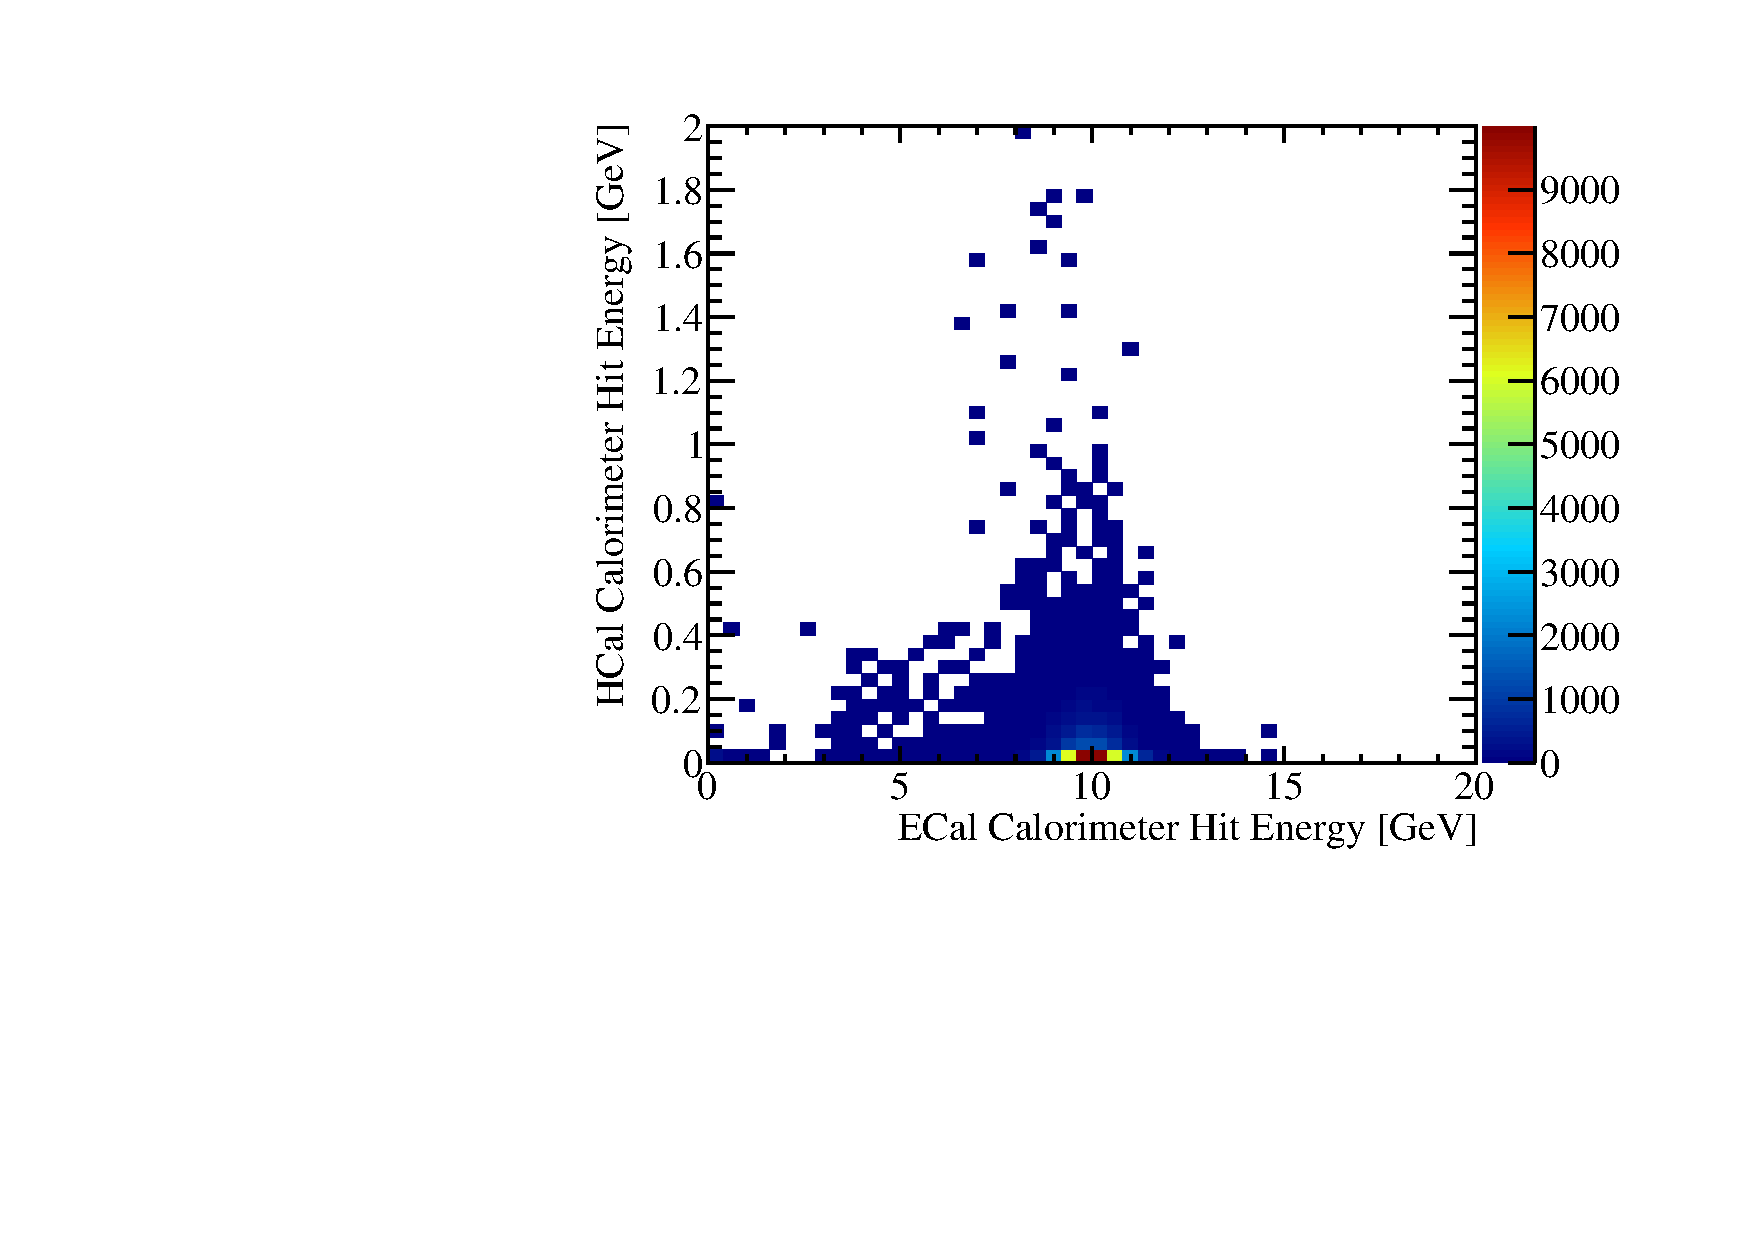
\includegraphics[width=0.5\textwidth]{EnergyEstimators/Plots/Calibration/Digitsation/ECal/ECalHCalPhotonSplit.pdf}
\caption[The sum of calorimeter hit energies in ECal and HCal for 10 GeV $\gamma$ events.]{The sum of calorimeter hit energies in ECal and HCal for 10 GeV $\gamma$ events.}
\label{fig:ecaldigiphotonsplit}
\end{figure}

Events are only used for calibrating the ECal digitisation if they are confined to the ECal.  To that extent cuts are applied ensuring that the sum of any reconstructed energy found outside the ECal is less than 1\% of $E_{MC}$ and that the $\text{cos}(\theta) < 0.95$ where $\theta$ is the polar angle of the $\gamma$.  $\gamma$ conversions are also vetoed in this event sample at MC level.  The impact of these cuts on the sum of ECal hit energies for the $E_{MC} = 10$ GeV $\gamma$ events is shown in figure \ref{fig:ecaldigiselection}.

\begin{figure}
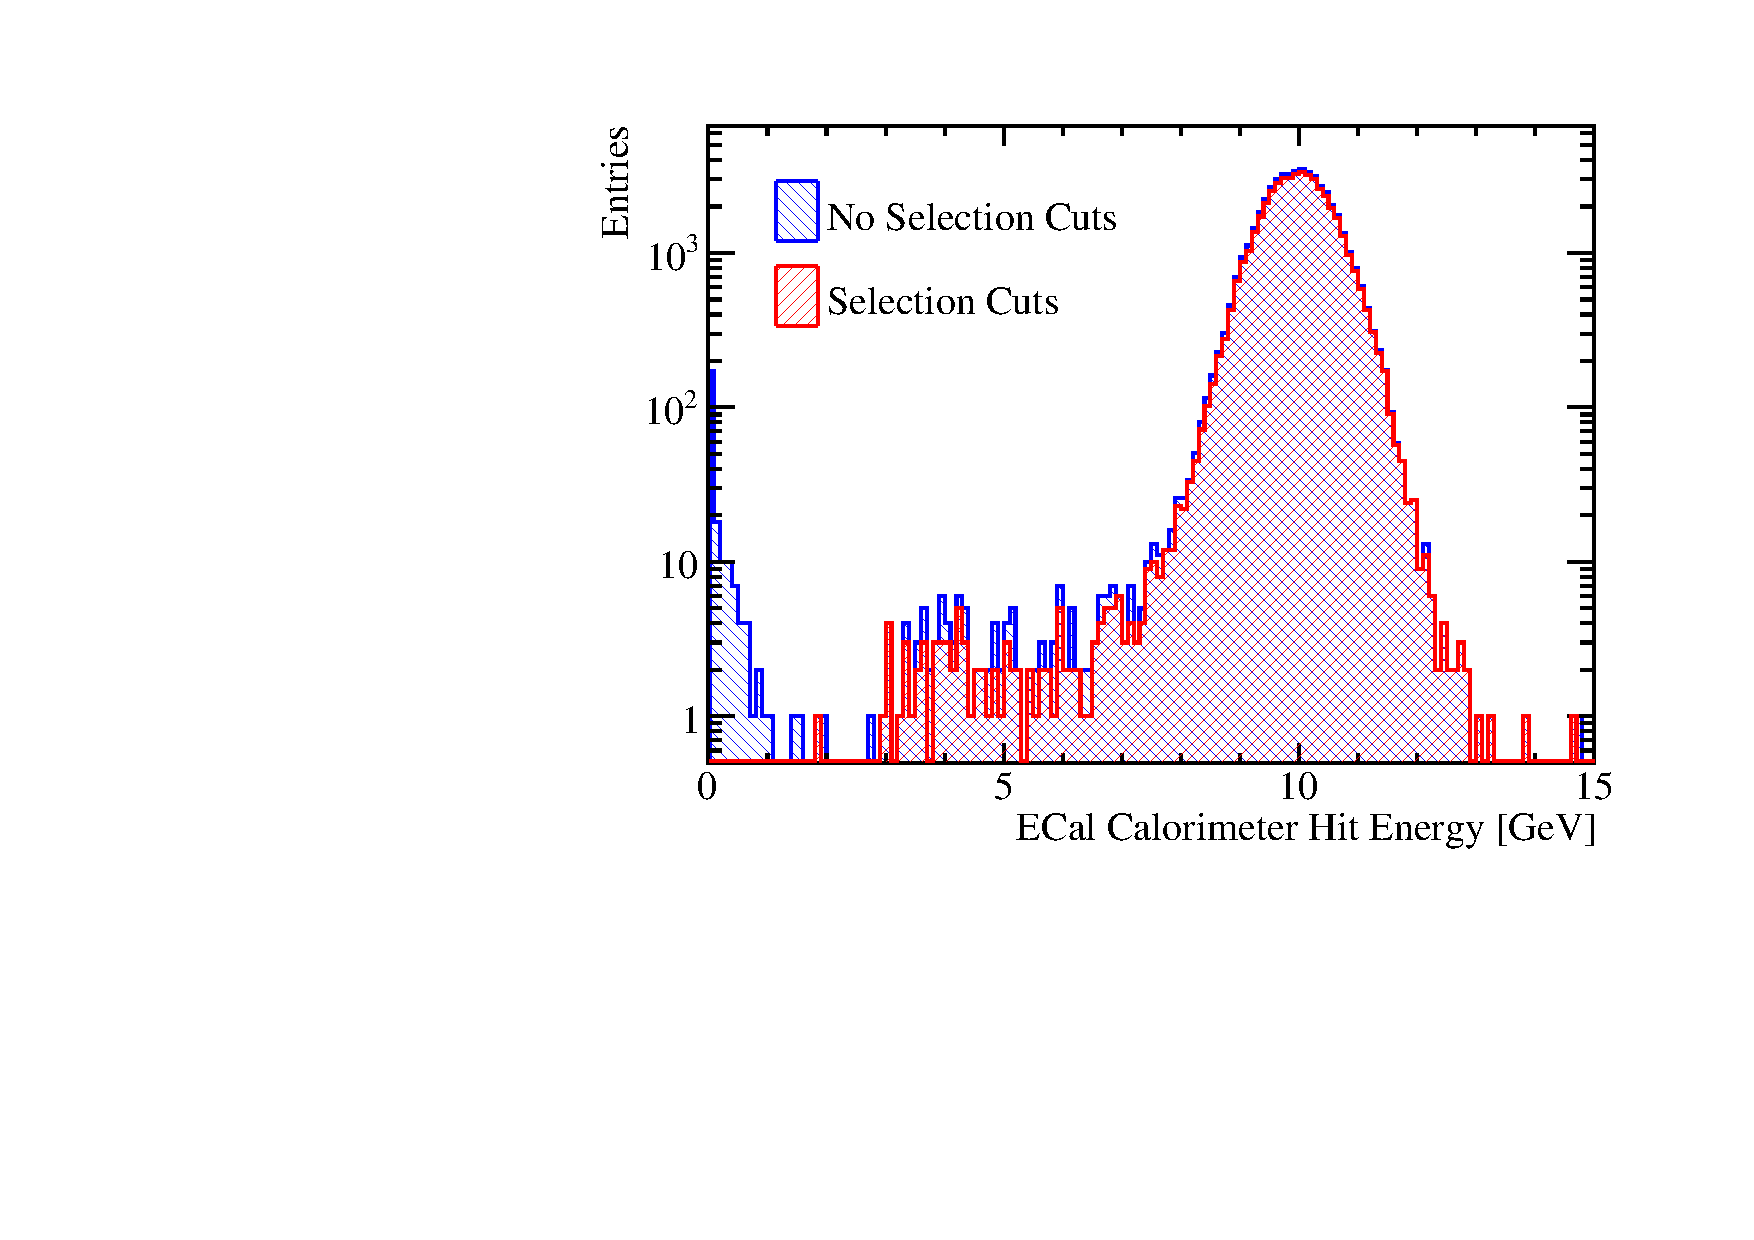
\includegraphics[width=0.5\textwidth]{EnergyEstimators/Plots/Calibration/Digitsation/ECal/DigitisationECalSelection.pdf}
\caption[The sum of the ECal calorimeter hit energies for 10 GeV $\gamma$ events with and without the selection cuts.]{The sum of the ECal calorimeter hit energies for 10 GeV $\gamma$ events with and without the selection cuts.}
\label{fig:ecaldigiselection}
\end{figure}

\begin{figure}
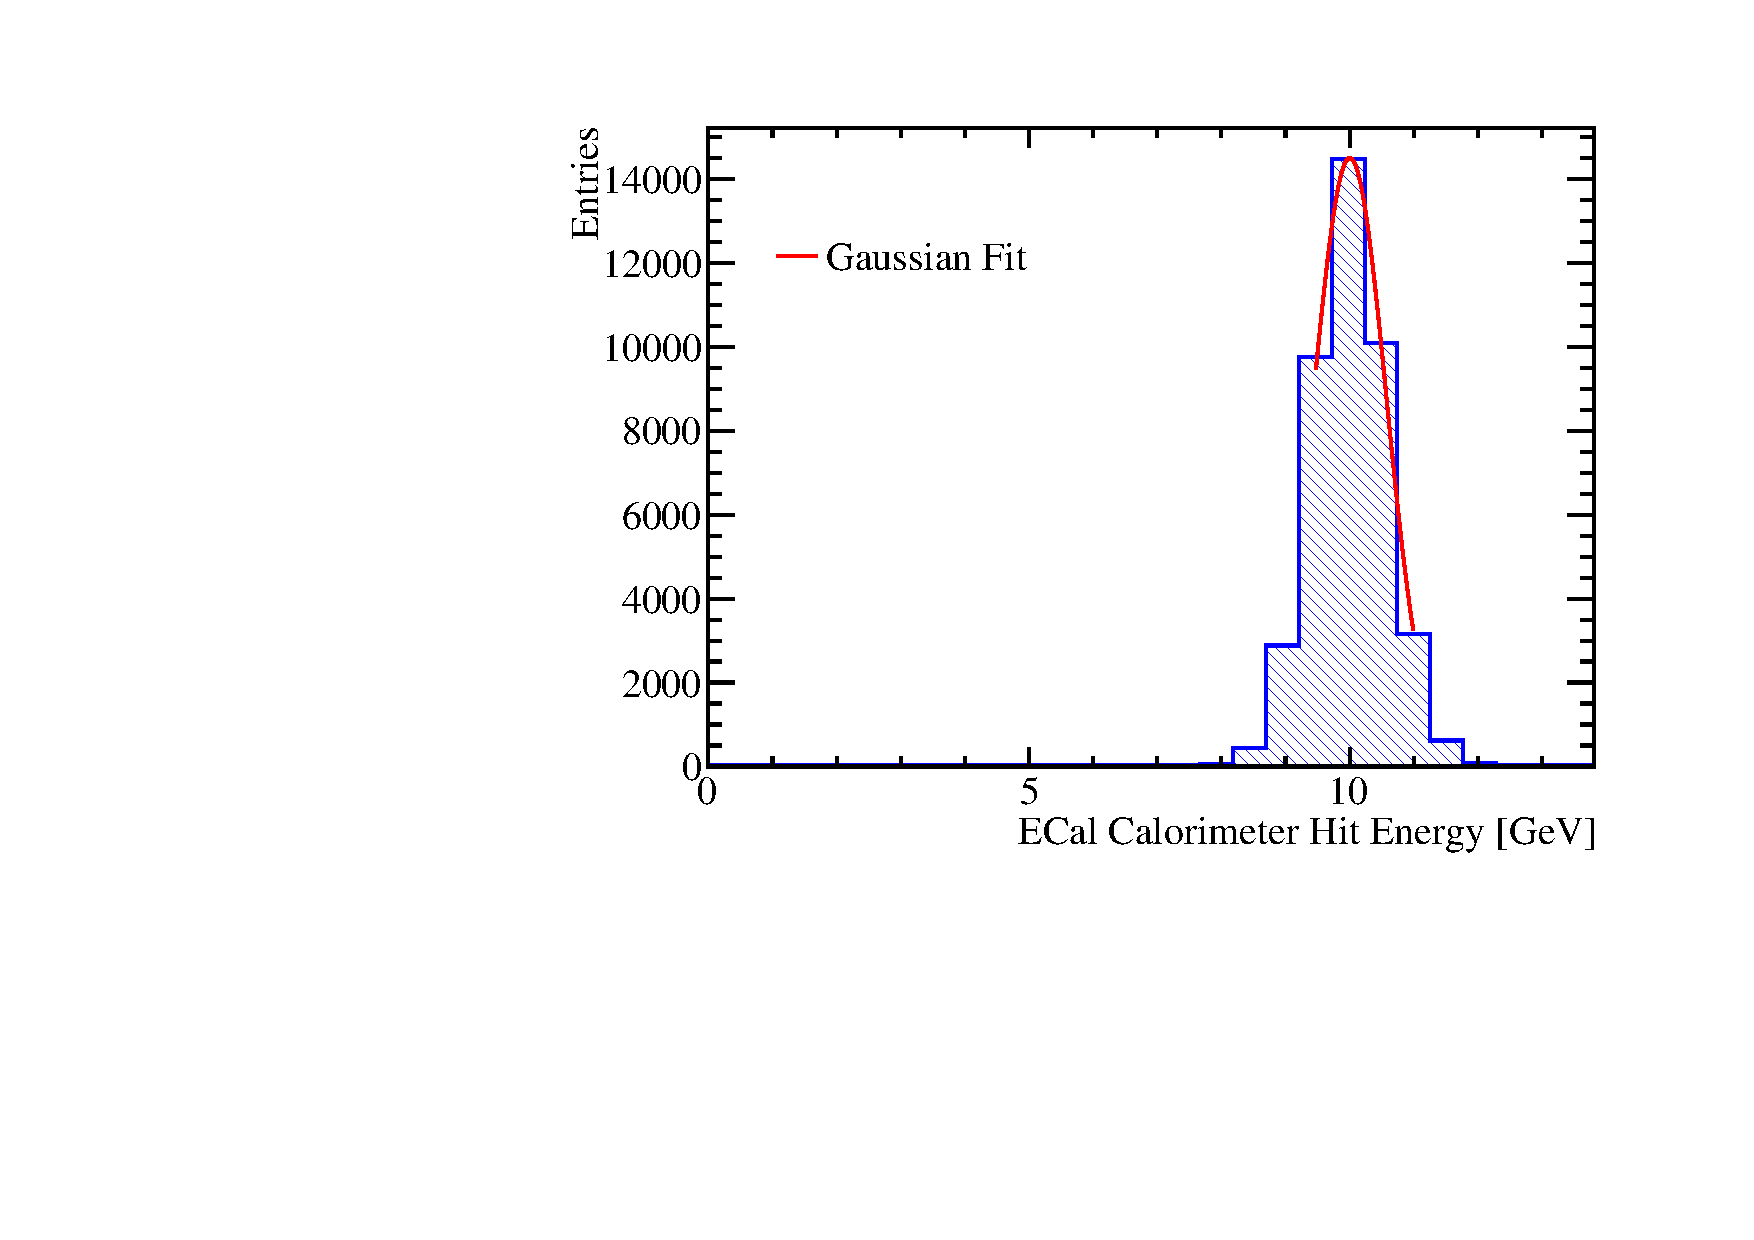
\includegraphics[width=0.5\textwidth]{EnergyEstimators/Plots/Calibration/Digitsation/ECal/DigitisationECalFit.pdf}
\caption[Gaussian fit to sum of the ECal calorimeter hit energies for 10 GeV $\gamma$ events with selection cuts.]{Gaussian fit to sum of the ECal calorimeter hit energies for 10 GeV $\gamma$ events with selection cuts.}
\label{fig:ecaldigifit}
\end{figure}

The calibration of the digitisation in the ECal is an iterative procedure and begins with the simulation of single $\gamma$ events using a trial calibration, with digitisation constant in the ECal $\alpha^{0}_{\text{ECal}}$ that may not be ideal.  Next the distribution of the sum of calorimeter hit energies within the ECal is produced for events passing the selection cuts, as shown in figure \ref{fig:ecaldigiselection}.  For an ideal calorimeter this distribution should be Gaussian, as was described in section CALORIMETER CHAPTER, therefore, a Gaussian fit is applied to this distribution and the mean, $E_{\text{Fit}}$, extracted.  To remove the effect of any outliers in this distribution, the fit is applied to the range of data with the smallest root mean square that contains at least 90 \% of the data.  An example of such a fit is shown in figure \ref{fig:ecaldigifit}.  In the case of ideal calibration the mean of this fit, $E_{\text{Fit}}$, would be equal $E_{MC}$.  It is assumed that any difference between the two is due to the calibration and to correct for this the digitisation constant from the trial calibration, $\alpha^{0}_{\text{ECal}}$, is rescaled by the ratio of the $E_{MC}$ to $E_{\text{Fit}}$.

\begin{equation}
\alpha^{0}_{\text{ECal}} \rightarrow \alpha_{\text{ECal}} = \alpha^{0}_{\text{ECal}} \times \frac{E_{MC}}{E_{Fit}}
\end{equation}

This procedure is then repeated until the $E_{\text{Fit}}$ falls within a specified tolerance.  The tolerance applied here was $|E_{\text{Fit}} - E_{\text{MC}}| < E_{\text{MC}} \times 5 \%$.  The binning used for the fitted histogram is chosen such that the bin width is equal to the desired tolerance on $E_{\text{Fit}}$ e.g. $E_{\text{MC}} \times 5 \% = 0.5$ GeV.  This tolerance is somewhat loose, however, it is tight enough to ensure successful application of PFA.  It should also be emphasised that the PFO energies used in downstream analyses have the electromagnetic and hadronic energy scale corrections applied, which are calibrated to a much tighter accuracy.

%========================================================================================

\subsubsection{HCal Digitisation}
\label{sec:hcaldigi}
The calibration for the digitisation in the HCal proceeds in a similar manor to that described for the ECal with a few key differences.  This calibration uses $K^{0}_{L}$ events at $E_{MC} = 20$ GeV as these neutral hadrons will deposit the bulk of their energy in the HCal.  The higher energy is used to create larger particle showers and sample deeper into the calorimeters.  

As in these events the $K^{0}_{L}$s have to pass through the ECal before arriving at the HCal and as the ECal contains $\approx 1 \lambda_{I}$, some of the $K^{0}_{L}$ begin showering in the ECal, as shown by figure \ref{fig:hcaldigikaonsplit}.  Such events are unsuitable for calibration of the HCal digitisation constants as rescaling $\alpha^{0}_{\text{HCal}}$ would not lead to a linear rescaling in $E_{\text{Fit}}$.  These events are vetoed in the even selections by applying selection cuts to ensure events used for the calibration deposit the bulk of their energy in the HCal.  

\begin{figure}
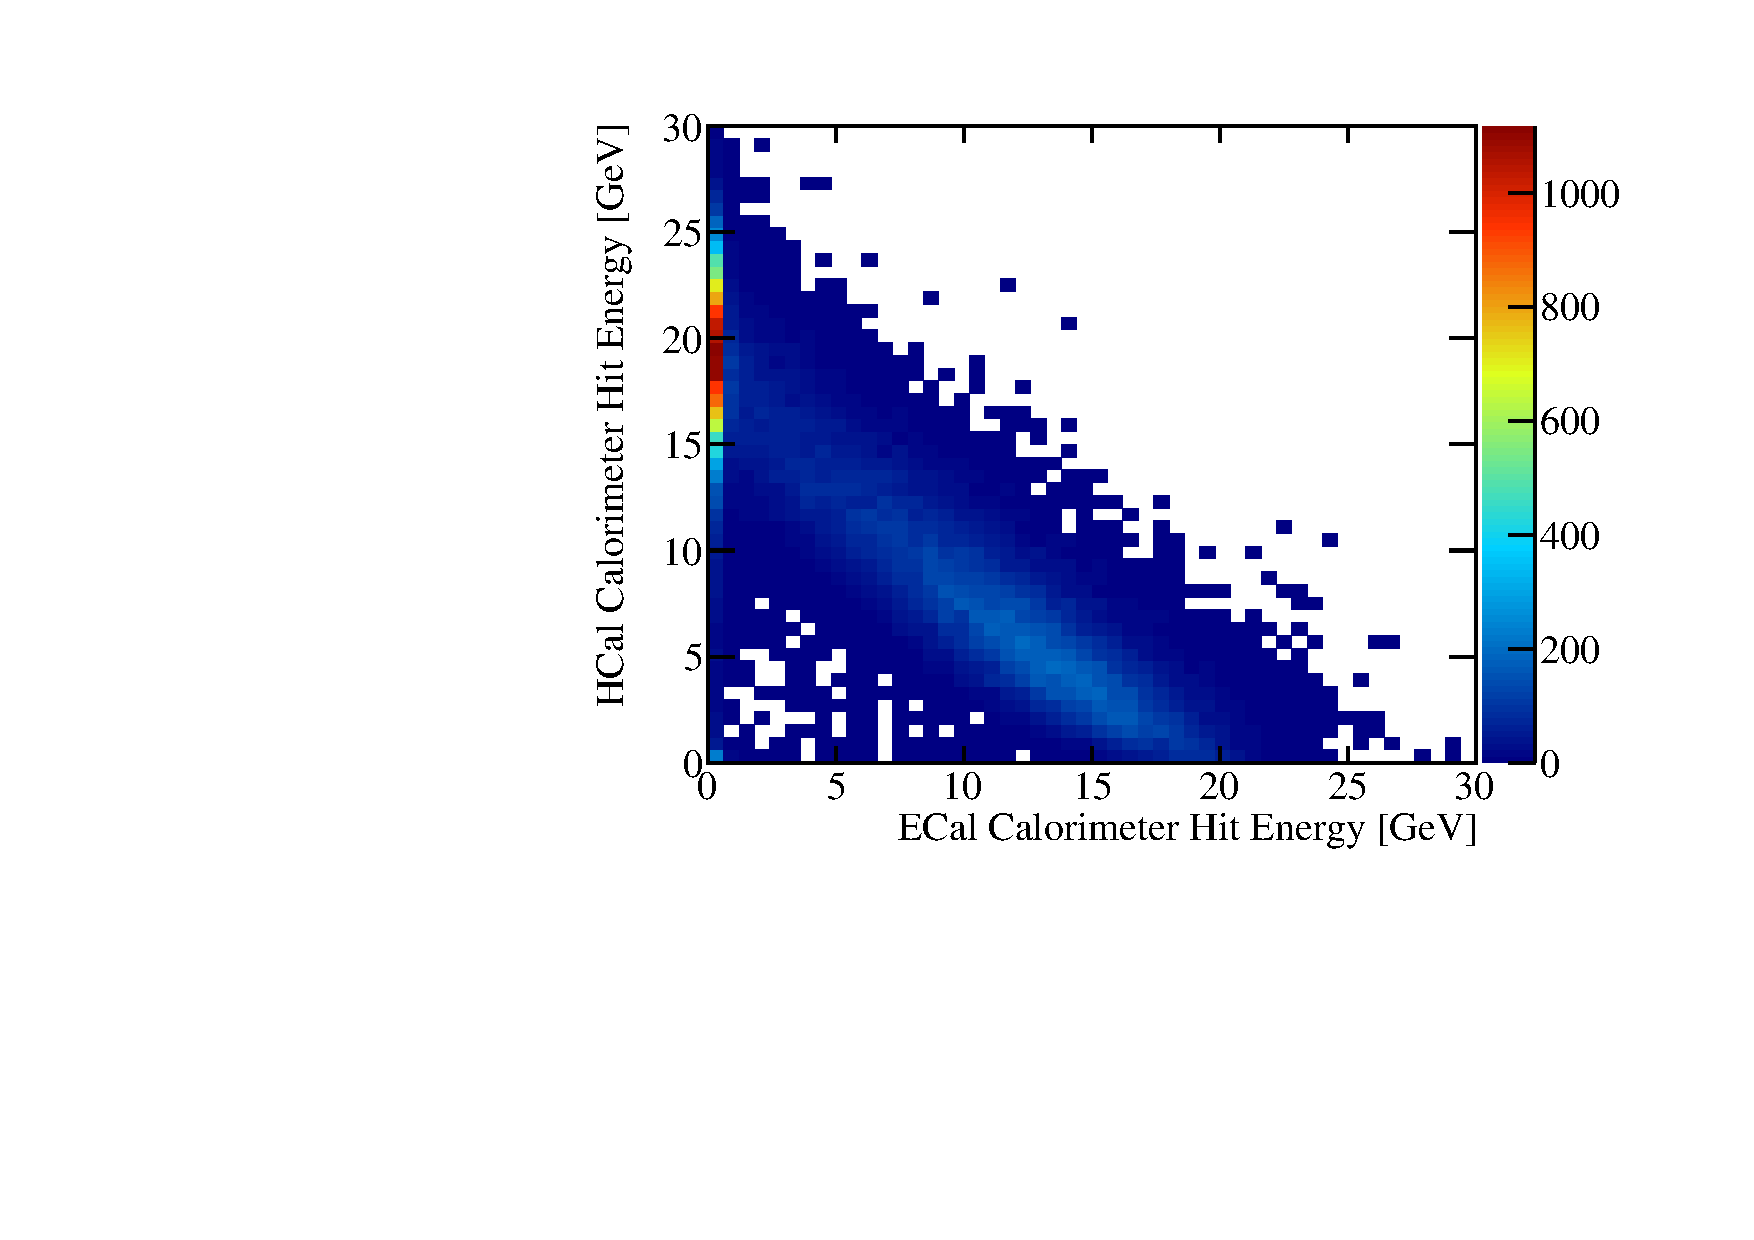
\includegraphics[width=0.5\textwidth]{EnergyEstimators/Plots/Calibration/Digitsation/HCal/ECalHCalKaon0LSplit.pdf}
\caption[Sum of calorimeter hit energies in ECal and HCal for 20 GeV $K^{0}_{L}$ events.]{Sum of calorimeter hit energies in ECal and HCal for 20 GeV $K^{0}_{L}$ events.}
\label{fig:hcaldigikaonsplit}
\end{figure}

Events are only considered in this analysis if a single neutral hadron PFO is reconstruction, the sum of any reconstructed energy found outside the HCal is less than 5\% of $E_{MC}$ and the last layer of the HCal where energy is deposited is in the first 90\% of the HCal.  The cut on the last HCal layer where energy is deposited is applied to veto events that shower late in the HCal and deposit a significant amount of energy in the uninstrumented coil region of the detector.  The impact of these cuts on the sum of HCal calorimeter hit energies for the $E_{MC} = 20$ GeV $K^{0}_{L}$ events is shown in figure \ref{fig:hcaldigiselection}.

\begin{figure}
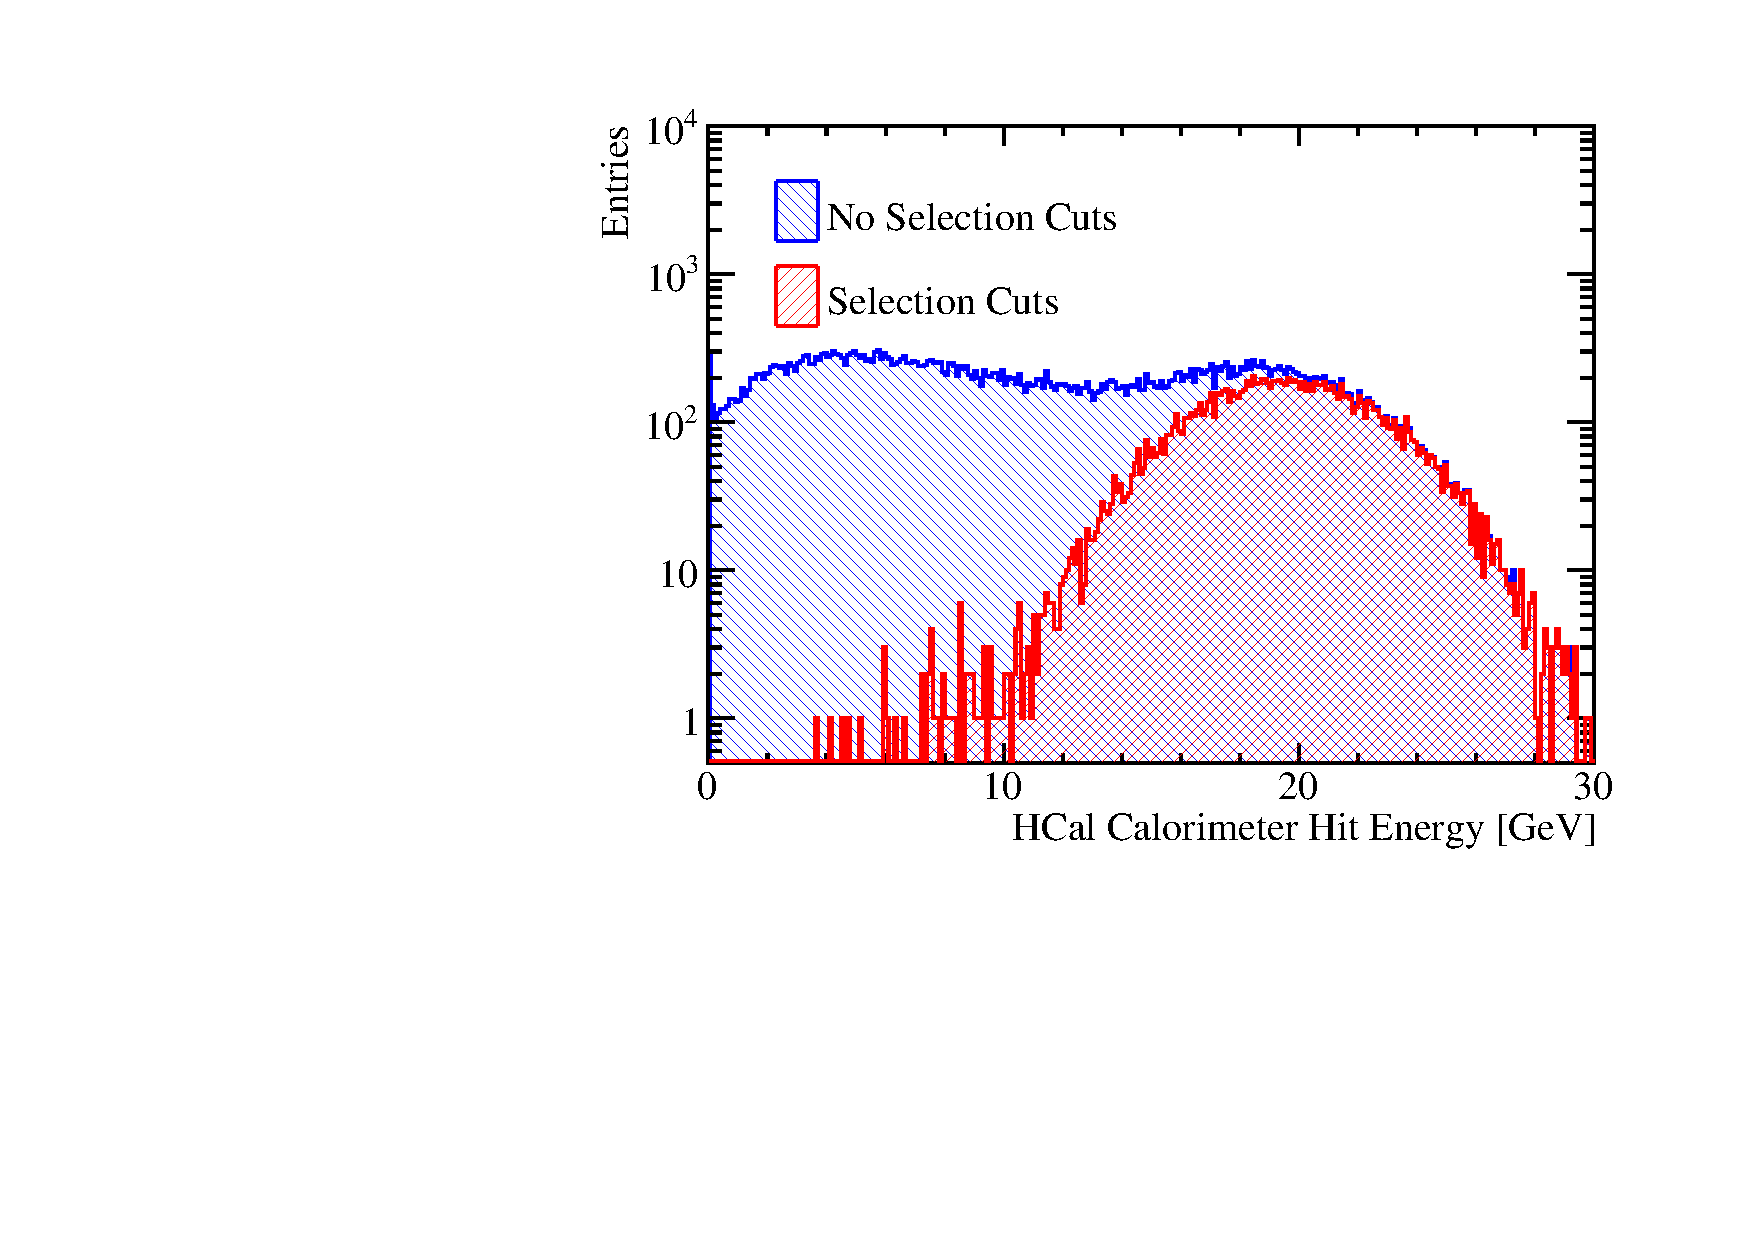
\includegraphics[width=0.5\textwidth]{EnergyEstimators/Plots/Calibration/Digitsation/HCal/DigitisationHCalSelection.pdf}
\caption[Sum of the HCal calorimeter hit energies for a 20 GeV $K^{0}_{L}$ events with and without the selection cuts.]{Sum of the HCal calorimeter hit energies for a 20 GeV $K^{0}_{L}$ events with and without the selection cuts.}
\label{fig:hcaldigiselection}
\end{figure}

There are two HCal digitisation constants used in the detector simulation, one applied for the Barrel and another for the EndCap.  This is to account for differences in hadronic shower dynamics between the two, such as differing magnetic field configurations in the Barrel and EndCap.  Both parameters are calibrated in the same manor, but have different cuts on $\theta$, the polar angle of the $K^{0}_{L}$.  For the Barrel region of the HCal events are selected if $0.2 < \text{cos}(\theta) < 0.6$, while for the EndCap events are selected if $0.8 < \text{cos}(\theta) < 0.9$.  These angular cuts are conservative to account for the transverse profile of the hadronic showers and ensure that they are confined to the relevant sub-detector.

Using these cuts the calibration procedure for the digitisation of the HCal Barrel and EndCap proceeds in the same manor as was described for the ECal, the details of which can be found in section \ref{sec:ecaldigi}.  Examples of the Gaussian fits applied to the sum of the calorimeter hit energies in the HCal Barrel and EndCap can be found in figure \ref{fig:hcaldigifit}.  

A noteworthy difference to the ECal digitisation procedure is that the target reconstructed energy for the $K^{0}_{L}$ samples is the kinetic energy as opposed to the total energy.  This decision was made as the majority of the neutral hadrons appearing in jets are neutrons and their accessible energy, what they can deposit in the detector, is their kinetic energy and not their rest mass energy.  This is the case as neutrons will come to a rest rather than decaying in the detector.  Therefore, calibrating to the kinetic energy should give the best performance for jet reconstruction.  

\begin{figure}
\subfloat[HCal Barrel.]{\label{fig:hcaldigibarrel}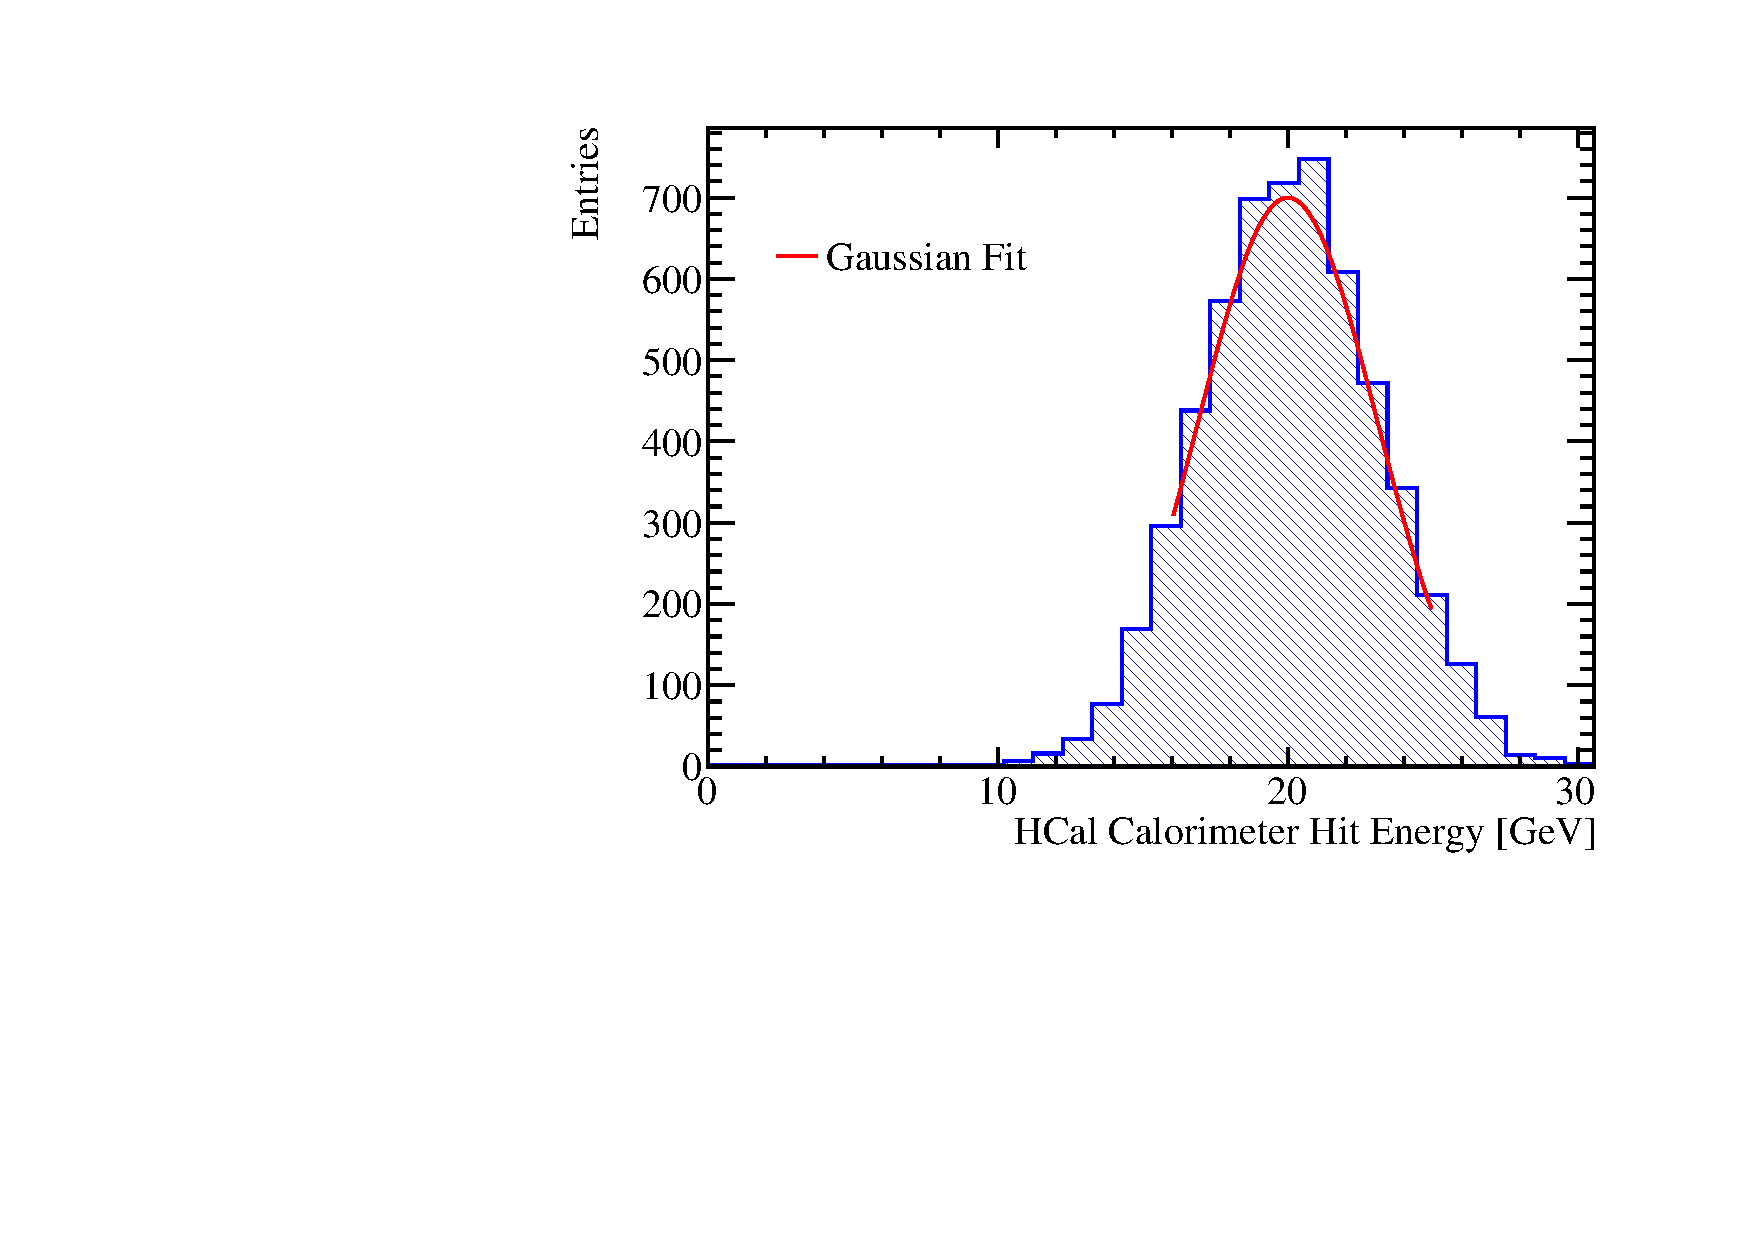
\includegraphics[width=0.5\textwidth]{EnergyEstimators/Plots/Calibration/Digitsation/HCal/DigitisationHCalBarrelFit.pdf}}
\subfloat[HCal EndCap.]{\label{fig:hcaldigiendcap}\includegraphics[width=0.5\textwidth]{EnergyEstimators/Plots/Calibration/Digitsation/HCal/DigitisationHCalEndCapFit.pdf}}
\caption[Gaussian fit to sum of the HCal calorimeter hit energies for 20 GeV $K^{0}_{L}$ events with selection cuts.]{Gaussian fit to sum of the HCal calorimeter hit energies for 20 GeV $K^{0}_{L}$ events with selection cuts.}
\label{fig:hcaldigifit}
\end{figure}

%========================================================================================

\subsubsection{HCal Ring Digitisation}
\label{sec:hcalringdigi}

\begin{figure}
\subfloat[]{\label{fig:ecal}\includegraphics[width=0.33\textwidth]{EnergyEstimators/Plots/Calibration/VisualDisplay/ECal.png}}
\subfloat[]{\label{fig:hcal}\includegraphics[width=0.33\textwidth]{EnergyEstimators/Plots/Calibration/VisualDisplay/HCal.png}}
\subfloat[]{\label{fig:hcalring}\includegraphics[width=0.33\textwidth]{EnergyEstimators/Plots/Calibration/VisualDisplay/HCalRing.png}}
\caption[A PandoraPFA event display showing the nominal ILD calorimeters.  \protect\subref{fig:ecal} show the ECal, \protect\subref{fig:hcal} shows the full HCal and \protect\subref{fig:hcalring} shows the HCal Ring.]{A PandoraPFA event display showing the nominal ILD calorimeters.  \protect\subref{fig:ecal} show the ECal, \protect\subref{fig:hcal} shows the full HCal and \protect\subref{fig:hcalring} shows the HCal Ring.}
\label{fig:calorimeters}
\end{figure}

The HCal Ring, illustrated in figure \ref{fig:calorimeters}, also has an independent digitisation constant to account for any difference in the hadronic shower development between the Ring, Barrel and EndCap.  The procedure used to calibrate this constant has to differs from that presented in section \ref{sec:hcaldigi} as it is unfeasible, due to the depth of the ring, to produce events that are wholly contained within it.  Fortunately, the size of the HCal ring means it plays a minimal role in the reconstruction, so precise calibration is not crucial.  To ensure that the calibration is approximately correct for the HCal Ring, $\alpha_{\text{HCal Ring}}$ is assumed to equal $\alpha_{\text{HCal EndCap}}$ multiplied by several factors designed to accounts for changes in the active layer thickness, absorber layer thickness and the MIP response between the HCal EndCap and Ring.  In detail:

\begin{equation}
\alpha_{\text{HCal Ring}} = \alpha_{\text{HCal EndCap}} \times \frac{\langle \text{cos}(\theta_\text{EndCap}) \rangle}{\langle \text{cos}(\theta_\text{Ring}) \rangle} \times \frac{P_\text{EndCap} }{P_\text{Ring} } \times \frac{L^{Absorber}_\text{EndCap}}{L^{Absorber}_\text{Ring} } \times \frac{L^{Active}_\text{Ring}}{L^{Active}_\text{EndCap}}
\end{equation}

where $\theta$ is the incident angle of the incoming particle to the calorimeter cells determined using the 20 GeV $K^{0}_{L}$ events, $L^{Active}$ is the active layer thickness and $L^{Absorber}$ is the absorber layer thickness. $P$ is the position of the MIP peak in the distribution of active layer cell energies, which has been corrected so that the MIP appears to enter the cell at normal incidence, and is determined using 10 GeV $\mu^{-}$ events.  Details on how $P$ is determined can be found in section \ref{sec:mipresponse}.

%========================================================================================

\subsection{MIP Scale Setting}
\label{sec:mipresponse}
The response of the various sub-detectors to a MIP has to be determined for both the digitisation processor and for PandoraPFA as both apply cuts in units of MIP response.  The digitiser applies cuts related to the electronic readout range of the various active layer technology options and applies a threshold on the minimum active layer energy for the creation of calorimeter hits.  PandoraPFA applies cuts designed to veto noise that would be present in a real detector.  Both these MIP responses, while intrinsically linked, have to be calculated separately as the digitiser requires the MIP peak definition from the active layer cell energies while, PandoraPFA requires the definition from the full cell, active and absorber layer, energies.  In these studies a MIP was defined as a 10 GeV $\mu^{-}$ \cite{Bichsel:2004ej} and no selection cuts applied to the sample.  

For the digitiser the MIP scale was defined as the, non-zero, peak in the distribution of the active layer calorimeter cell energies for normally incident $\mu^{-}$ as shown in figure \ref{fig:digitisermip}.  This distribution was produced using a sample of $\mu^{-}$ events that are spatially isotropic about the impact point.  A direction correction factor, $\text{cos}(\theta)$ where $\theta$ is the incident angle of the incoming $\mu^{-}$ to the calorimeter cell, was applied to the active layer cell energies to generate the effect of having normally incident $\mu^{-}$.  

\begin{figure}
\subfloat[ECal.]{\label{fig:digitisermipecal}\includegraphics[width=0.5\textwidth]{EnergyEstimators/Plots/Calibration/MIPScale/Digitiser/MIPScaleDigitiserECal.pdf}}
\subfloat[HCal Barrel.]{\label{fig:digitisermiphcalbarrel}\includegraphics[width=0.5\textwidth]{EnergyEstimators/Plots/Calibration/MIPScale/Digitiser/MIPScaleDigitiserHCalBarrel.pdf}} \\
\subfloat[HCal EndCap.]{\label{fig:digitisermiphcalendcap}\includegraphics[width=0.5\textwidth]{EnergyEstimators/Plots/Calibration/MIPScale/Digitiser/MIPScaleDigitiserHCalEndCap.pdf}}
\subfloat[HCal Ring.]{\label{fig:digitisermiphcalring}\includegraphics[width=0.5\textwidth]{EnergyEstimators/Plots/Calibration/MIPScale/Digitiser/MIPScaleDigitiserHCalOther.pdf}}
\caption[The active layer calorimeter cell energy distributions for \protect\subref{fig:digitisermipecal} the ECal, \protect\subref{fig:digitisermiphcalbarrel} the HCal Barrel, \protect\subref{fig:digitisermiphcalendcap} the HCal EndCap and \protect\subref{fig:digitisermiphcalring} the HCal Ring for 10 GeV $\mu^{-}$ events.]{The active layer calorimeter cell energy distributions for \protect\subref{fig:digitisermipecal} the ECal, \protect\subref{fig:digitisermiphcalbarrel} the HCal Barrel, \protect\subref{fig:digitisermiphcalendcap} the HCal EndCap and \protect\subref{fig:digitisermiphcalring} the HCal Ring for 10 GeV $\mu^{-}$ events.}
\label{fig:digitisermip}
\end{figure}

In the digitiser processor a single value for the MIP peak was required for the HCal and that was taken as the MIP peak position for the HCal Barrel.  The MIP peaks were separately calculated for the HCal EndCap and Ring for the purposes of the HCal Ring digitisation described in section \ref{sec:hcalringdigi}.  The realistic digitisation features present in the simulation of the ECal and HCal are not available for the muon chamber simulation, therefore, no MIP peak setting for that digitisation step is required.

A similar procedure was employed for calculation of the MIP peak in PandoraPFA.  One important difference was the distribution used for setting the MIP scale in PandoraPFA is the distribution of calorimeter cell energies, i.e. the energy in the active and absorber layers of a cell, and not just the active layer energies.  Examples of the distributions used to set the MIP scale in PandoraPFA can be found in figure \ref{fig:pandoramip}.  There are few populated low calorimeter cell energy bins due to cuts applied in the digitiser on the minimum active layer energy required to make a calorimeter hit.  The double peak structure in the ECal calorimeter hit energy distribution is present due to the doubling of the thickness of the ECal absorber material, from 2.1 mm to 4.2 mm tungsten, in the ILD detector model that occurs for the back 10 layers of the 30 layer ECal.  Further differences between the MIP scale setting in the digitiser and PandoraPFA worthy of note are that in PandoraPFA the HCal MIP scale setting combines the HCal sub-detectors, the Barrel, EndCal and Ring, together and PandoraPFA requires the MIP scale to be set in the muon chamber, which requires the muon chamber cell energy distribution to be created.  

\begin{figure}
\subfloat[]{\label{fig:pandoramipecal}\includegraphics[width=0.5\textwidth]{EnergyEstimators/Plots/Calibration/MIPScale/PandoraPFA/MIPScalePandoraPFAECal.pdf}}
\subfloat[]{\label{fig:pandoramiphcal}\includegraphics[width=0.5\textwidth]{EnergyEstimators/Plots/Calibration/MIPScale/PandoraPFA/MIPScalePandoraPFAHCal.pdf}} \\
\subfloat[]{\label{fig:pandoramipmuon}\includegraphics[width=0.5\textwidth]{EnergyEstimators/Plots/Calibration/MIPScale/PandoraPFA/MIPScalePandoraPFAMuon.pdf}}
\caption[The calorimeter cell energy distributions for \protect\subref{fig:pandoramipecal} the ECal, \protect\subref{fig:pandoramiphcal} the HCal and \protect\subref{fig:pandoramipmuon} the muon chamber for 10 GeV $\mu^{-}$ events.]{The calorimeter cell energy distributions for \protect\subref{fig:pandoramipecal} the ECal, \protect\subref{fig:pandoramiphcal} the HCal and \protect\subref{fig:pandoramipmuon} the muon chamber for 10 GeV $\mu^{-}$ events.}
\label{fig:pandoramip}
\end{figure}

%========================================================================================

\subsection{Electromagnetic and hadronic scale setting}
\label{sec:scalesetting}
The electromagnetic and hadronic scales have to be independently set in the simulation to account for the different mechanisms governing the propagation of electromagnetic and hadronic showers.  The setting of the scales involves tuning four parameters in PandoraPFA that correspond to energy rescaling factors, which are applied to energy measurements from electromagnetic and hadronic showering particles in the ECal and HCal.  

%========================================================================================

\subsubsection{Electromagnetic scale setting}
\label{sec:emscalesetting}
The electromagnetic scale in the ECal, $\beta^{EM}_{ECal}$, is determined using $\gamma$ events at $E_{MC} = 10$ GeV.  $\gamma$ events are ideal for the setting of the electromagnetic scale as they procedure electromagnetic showers and are primarily confined to the ECal at the energy considered, which was shown in figure \ref{fig:ecaldigiphotonsplit}.  

Cuts are applied to ensure that only events where the bulk of the energy is deposited within the ECal are used for this part of the calibration.  Less than 1\% of the reconstructed energy is outside the ECal to ensure the event is contained.  Furthermore, cuts requiring a single $\gamma$ be reconstructed are added to veto pattern recognition failures.  $\gamma$ conversions are excluded at MC level to ensure energy measurements used in the calibration arise from the calorimeters and not the charged particle tracks.  The impact of these cuts on the electromagnetic energy measured in the ECal for 10 GeV $\gamma$ events is shown in figure \ref{fig:ecalemscaleselection}.

\begin{figure}
\includegraphics[width=0.5\textwidth]{EnergyEstimators/Plots/Calibration/EMScaleSetting/EMScaleECalSelection.pdf}
\caption[Sum of the electromagnetic energy measured in the ECal for 10 GeV $\gamma$ events with and without the selection cuts.]{Sum of the electromagnetic energy measured in the ECal for 10 GeV $\gamma$ events with and without the selection cuts.}
\label{fig:ecalemscaleselection}
\end{figure}

\begin{figure}
\includegraphics[width=0.5\textwidth]{EnergyEstimators/Plots/Calibration/EMScaleSetting/EMScaleSettingECalFit.pdf}
\caption[Gaussian fit to sum of the electromagnetic energy deposited in the ECal for 10 GeV $\gamma$ events with selection cuts.]{Gaussian fit to sum of the electromagnetic energy deposited in the ECal for 10 GeV $\gamma$ events with selection cuts.}
\label{fig:ecalemscalefit}
\end{figure}

The fitting procedure follows that used for the ECal digitisation, described in section \ref{sec:ecaldigi}, whereby a trial calibration for the electromagnetic energy scale in the ECal, $\beta^{EM0}_{ECal}$, is assumed and the single $\gamma$ events simulated.  The distribution of the electromagnetic energy in the ECal is created and a Gaussian fit applied to the range of data with the smallest root mean square containing at least 90 \% of the data.  The mean of this fit, $E_{\text{Fit}}$, is then used to scale $\beta^{EM0}_{ECal}$ in the following way

\begin{equation}
\beta^{EM0}_{ECal} \rightarrow \beta^{EM}_{ECal} = \beta^{EM0}_{ECal} \times \frac{E_{MC}}{E_{Fit}}
\end{equation}

An example distribution and fit used in the calibration of the nominal ILD detector model can be found in figure \ref{fig:ecalemscalefit}.  This procedure is repeated using the updated $\beta^{EM}_{ECal}$ until $E_{\text{Fit}}$ falls within a specified tolerance.  The tolerance applied here was $|E_{\text{Fit}} - E_{\text{MC}}| < E_{\text{MC}} \times 0.5 \%$.  The binning for the fitted histogram is chosen such that the bin width is equal to the desired target tolerance on $E_{\text{Fit}}$ e.g. $E_{\text{MC}} \times 0.5 \% = 0.05$ GeV.  This tolerance is tighter than was applied for the digitisation as it is these energies that are used in downstream analyses.   
 
The electromagnetic scale in the HCal, $\beta^{EM}_{HCal}$, is chosen to be equal to the hadronic scale in the HCal, $\beta^{Had}_{HCal}$.  The details of the determination of $\beta^{Had}_{HCal}$ can be found in section \ref{sec:hadscalesetting}.  For the ILC and CLIC, $\beta^{EM}_{HCal}$ is not a critical parameter in the reconstruction as photons are largely contained within the ECal meaning little to no electromagnetic energy is measured in the HCal.  

%========================================================================================

\subsubsection{Hadronic scale setting}
\label{sec:hadscalesetting}
The hadronic scale in the ECal, $\beta^{Had}_{ECal}$, is important to detector performance as a non-negligible amount of hadronic energy will be measured in the ECal.  As the ECal contains $\approx 1 \lambda_{I}$, the hadronic scale in the ECal cannot be independently set as it is unfeasible to create a large sample of 20 GeV $K^{0}_{L}$ events that are fully contained within it.  Therefore, the hadronic scale in the ECal and HCal have to be set simultaneously.  

Cuts are applied to select the $K^{0}_{L}$ events that are appropriate to use for the hadronic scale calibration.  The last layer in which energy is deposited in the HCal must not occur in the back 10 \% of the HCal.  This ensures that the event does not suffer from leakage of energy out of the back of the HCal.  A single neutral hadron must be reconstructed to veto events with reconstruction failures.  Finally, the total hadronic energy measured in ECal and HCal, $E^{Had}_{ECal} + E^{Had}_{HCal}$, must fall within 3 $\sigma$ of the desired hadronic energy distribution, $E^{Had}_{ECal} + E^{Had}_{HCal} = 20 \text {GeV} - m_{K^{0}_{L}} = E_{K}$.  $\sigma$ is defined to be $55\% \times \sqrt{E} = 2.46 \text{GeV}$ for 20 GeV $K^{0}_{L}$.  This definition for sigma is used as it matches the energy resolution as a function of energy for neutral hadrons using the nominal ILD HCal \cite{Behnke:2013lya}.  This cut ensures that when fitting the two dimensional distribution of hadronic energy measured in the ECal and HCal outliers do not skew the fit.  Once again the target reconstructed energy for this sample is the kinetic energy and not the total energy of the $K^{0}_{L}$ for the reasons outlined in section \ref{sec:hcaldigi}.  The impact of cuts are illustrated in figure \ref{fig:hadscaleselection}.

\begin{figure}
\subfloat[]{\label{fig:hadscaleselectionnocuts}\includegraphics[width=0.5\textwidth]{EnergyEstimators/Plots/Calibration/HadScaleSetting/HadScaleECalHCalSelectionNoCuts.pdf}}
\subfloat[]{\label{fig:hadscaleselectioncuts}\includegraphics[width=0.5\textwidth]{EnergyEstimators/Plots/Calibration/HadScaleSetting/HadScaleECalHCalSelectionCuts.pdf}}
\caption[The distribution of hadronic energy measured in the ECal and HCal for 20 GeV $K^{0}_{L}$ events with and without selection cuts.]{The distribution of hadronic energy measured in the ECal and HCal for 20 GeV $K^{0}_{L}$ events \protect\subref{fig:hadscaleselectionnocuts} without selection cuts and \protect\subref{fig:hadscaleselectioncuts} with selection cuts.}
\label{fig:hadscaleselection}
\end{figure}

This part of the calibration procedure is again iterative and begins by assuming trial values, $\beta^{Had0}_{ECal}$ and $\beta^{Had0}_{ECal}$, for the hadronic scale calibration factors $\beta^{Had}_{ECal}$ and $\beta^{Had}_{ECal}$.  The 20 GeV $K^{0}_{L}$ events are then simulated and reconstructed.  Following that a linear fit to the distribution of $E^{Had}_{ECal}$ against $E^{Had}_{HCal}$ for 20 GeV $K^{0}_{L}$ events passing the selection cuts is applied.  The fit is performed by minimising $\chi^{2}$, which is defined as

\begin{equation}
\chi^{2}(\delta^{Had}_{ECal}, \delta^{Had}_{HCal}) = \sum_{i} \frac{x_{i}}{\sigma_{x_{i}}}
\end{equation}

where $x_{i}$ is the perpendicular distance from $E^{Had}_{ECal}$ and $E^{Had}_{HCal}$ for event $i$ to the line $E^{Had}_{HCal} = \delta^{Had}_{HCal} - E^{Had}_{ECal} \frac{\delta^{Had}_{HCal}}{\delta^{Had}_{ECal}}$.   The definition of $x_{i}$ is given in equation \ref{equ:xicalc}, but best illustrated by considering figure \ref{fig:hadscalechi2calc}.  $\sigma_{x_{i}}$ is the uncertainty on $x_{i}$, which is calculated by propagating the uncertainties on $E^{Had}_{ECal}$ and $E^{Had}_{HCal}$, which are assumed to be $\sigma_{E^{Had}_{E/HCal}} = 55\% \times \sqrt{E^{Had}_{E/HCal}}$, into the expression for $x_{i}$.  The result of this propagation of errors is given in equation \ref{equ:sigmaxicalc}.  The sum runs over all events, $i$, passing the selection cuts.  

\begin{figure}
\includegraphics[width=0.5\textwidth]{EnergyEstimators/Plots/Calibration/HadScaleSetting/HadScaleECalHCalSelectionExample.pdf}
\caption[An example showing the definition of $x_{i}$, the variable used for the calculation of $\chi^{2}(\delta^{Had}_{ECal}, \delta^{Had}_{HCal})$ for the setting of the hadronic energy scale.]{An example showing the definition of $x_{i}$, the variable used for the calculation of $\chi^{2}$ for the setting of the hadronic energy scale.  For an event that has been measured with hadronic energy $E^{Had}_{ECal}$ in the ECal and $E^{Had}_{HCal}$ in the HCal, the geometric interpretation of $x_{i}$ is shown.  The blue dotted line is defined as $E^{Had}_{HCal} = \delta^{Had}_{HCal} - E^{Had}_{ECal} \frac{\delta^{Had}_{HCal}}{\delta^{Had}_{ECal}}$.}
\label{fig:hadscalechi2calc}
\end{figure}

\begin{equation}
x_{i} = \frac{E^{Had}_{HCal} \delta^{Had}_{ECal} + E^{Had}_{ECal} \delta^{Had}_{HCal} - \delta^{Had}_{ECal} \delta^{Had}_{HCal}}{\sqrt{(\delta^{Had}_{ECal})^{2} + (\delta^{Had}_{HCal})^{2}}}
\label{equ:xicalc}
\end{equation}

\begin{equation}
\sigma_{i} = \frac{(\sigma_{E^{Had}_{HCal}}  \delta^{Had}_{ECal})^{2} + (\sigma_{E^{Had}_{ECal}} \delta^{Had}_{HCal})^{2}}{\sqrt{(\delta^{Had}_{ECal})^{2} + (\delta^{Had}_{HCal})^{2}}}
\label{equ:sigmaxicalc}
\end{equation}

The minimisation is done by stepping a range of $\delta^{Had}_{ECal}$ and $\delta^{Had}_{HCal}$ centred about the ideal value of $20 \text { GeV} - m_{K^{0}_{L}}$ in search for the minimum $\chi^{2}$.  Once the minima in $\chi^{2}$ is found the trial calibration factors $\beta^{Had0}_{ECal}$ and $\beta^{Had0}_{ECal}$ are rescaled to correct for any deviation from the desired fit as follows

\begin{equation}
\beta^{Had0}_{ECal} \rightarrow \beta^{Had}_{ECal} = \beta^{Had0}_{ECal} \times \frac{E_{K}}{\Delta^{Had}_{ECal}} \\
\beta^{Had0}_{HCal} \rightarrow \beta^{Had}_{HCal} = \beta^{Had0}_{HCal} \times \frac{E_{K}}{\Delta^{Had}_{HCal}}
\end{equation}

where $\Delta^{Had}_{ECal}$ and $\Delta^{Had}_{ECal}$ are the values of $\delta^{Had}_{ECal}$ and $\delta^{Had}_{ECal}$ giving the minimum $\chi^{2}$.  The step sizes used for minimising $\chi^{2}$ with respect to $\delta^{Had}_{ECal}$ and $\delta^{Had}_{ECal}$ is chosen such that a single step corresponds to the target final tolerance on $\delta^{Had}$ i.e. $|\delta^{Had}_{E/HCal} - E_{\text{MC}}| < E_{\text{MC}} \times 0.5 \% \approx 0.1 \text{GeV}$.  

This procedure is then repeated until $\Delta^{Had}_{ECal}$ and $\Delta^{Had}_{ECal}$ both fall within a given tolerance, which in this case it taken to be $|\Delta^{Had}_{E/HCal} - E_{\text{MC}}| < E_{\text{MC}} \times 0.5 \% \approx 0.1 \text{GeV}$

%========================================================================================

\subsection{Calibration step ordering}
\label{sec:orderingcalib}

The calibration procedure has to be run in the following order so that the building blocks used for each stage of the calibration procedure can be assumed to be correctly calibrated:

\begin{enumerate}
\item MIP Scale setting in the digitiser as described in section \ref{sec:mipresponse}.
\item Calibration of digitisation of calorimeter hits in the ECal and HCal as described in section \ref{sec:digi}.
\item MIP Scale setting in PandoraPFA as described in section \ref{sec:mipresponse}.
\item Electromagnetic and hadronic scale settings in PandoraPFA as described in section \ref{sec:scalesetting}.
\end{enumerate}

%========================================================================================

\subsection{Retraining photon likelihood data}
PandoraPFA uses likelihood data in the identification of $\gamma$s.  Data related to the topology and energy of electromagnetic showers and the wider event environment is used to determine whether a given shower is likely to be a $\gamma$.  The likelihood data is trained using off-shell mass Z boson (Z') events at 500 GeV that decay into light quarks (u, d, s).  It is necessary to retrain this data only when varying the ECal as photons are contained largely within the ECal at the energies being considered and the likelihood data only uses measurements made in the ECal.

As this data uses post digitisation hits it is important to ensure that a fully calibrated detector is used when retraining the likelihood data.  Therefore, it is necessary to run the calibration procedure, as described in section \ref{sec:orderingcalib}, before retaining.  However, as the reconstruction uses likelihood data the calibration procedure must be performed twice.  Initially the calibration procedure is performed where PandoraPFA is run without the inclusion of this likelihood data, using PandoraSettingsMuon.xml.  Then the likelihood data is retrained using the results of the first calibration pass and then the retrained likelihood data is used in the second pass of the calibration procedure.  

In the optimisation studies presented in chapter OPTIMISATION STUDIES this procedure was followed whenever the ECal was modified so that optimal detector performance was achieved.  

%========================================================================================
%========================================================================================

\section{HCal Cell Truncation}
\label{sec:hcalcelltruncation}
A powerful tool used by PandoraPFA in event reconstruction is the application of a truncation to the maximum amount of energy that can be recorded in a calorimeter cell in the HCal.  The purpose of this truncation is to eliminate the effect of spuriously high energy calorimeter cells that would skew the reconstruction.  The origin of these high energy cells is twofold: showering particles may be moving within the plane of the active material, which can lead to an overestimation of the deposited energy if the shower is not sufficiently uniform across the full cell, and Landau fluctuations \cite{Landau:1944if}, which originate from high energy knock-on electrons appearing within particle showers \cite{Bichsel:2004ej}.  These effects are only relevant in hadronic showers as electromagnetic showers begin showering almost immediately within the ECal, meaning they are unlikely to be directed within the plane of the active material of the calorimeter, and the Landau distribution only describes the energy loss for charged particles.  This means showering $\gamma$ do not produce Landau fluctuations and neither do $e^{-}$ and $e^{+}$ as their energy, in the particle flow paradigm, arises from the curvature of the track they produce and not the calorimeter hits.  Therefor, as only hadronic showers produce spuriously high energy cells through these mechanisms, this truncation is only applied on HCal cells.  

A great deal of care has to be given to the truncation energy so that cells from typical hadronic shower development are not truncated, while the spuriously high energy cells are.  This can be illustrated by considering the single particle energy resolutions as a function of the HCal cell truncation that are shown in figure \ref{fig:ercelltrunc}.  The photon energy resolution is invariant to changes in the cell truncation as no photon energy is recorded in the HCal, while the energy resolution for the neutral hadrons is optimal for a truncation of 1 GeV.  This indicates that a  GeV truncation is sufficient for dealing with the Landau fluctuations and showering particles travelling within the active material of the calorimeter cell.  For cell truncations greater than 1 GeV the resolution degrades as the spuriously high energy cells are not accounted for, while truncations below 1 GeV truncate energy measurements from typical hadronic shower development.  If typical hadronic shower cells are truncated this leads to a poorer sampling of the shower and a degradation in the energy resolution.  

\begin{figure}
\subfloat[]{\label{fig:ercelltruncphotons}\includegraphics[width=0.5\textwidth]{EnergyEstimators/Plots/CellTruncation/ER_vs_PhotonCellTrunc_100GeVPhoton.pdf}}
\subfloat[]{\label{fig:ercelltrunckaons}\includegraphics[width=0.5\textwidth]{EnergyEstimators/Plots/CellTruncation/ER_vs_Kaon0LCellTrunc_50GeVKaon0L.pdf}}
\caption[The energy resolution as a function of HCal cell truncation for \protect\subref{fig:ercelltruncphotons} 100 GeV $\gamma$ events and \protect\subref{fig:ercelltrunckaons} 50 GeV $K^{0}_{L}$ events for the nominal ILD detector model.]{The energy resolution as a function of HCal cell truncation for \protect\subref{fig:ercelltruncphotons} 100 GeV $\gamma$ events and \protect\subref{fig:ercelltrunckaons} 50 GeV $K^{0}_{L}$ events for the nominal ILD detector model.}
\label{fig:ercelltrunc}
\end{figure}

Once again, this effect propagates into the jet energy resolutions as shown by figure \ref{fig:jercelltrunc}.  The trends in this plot are complex as the optimal cell truncation varies with the jet energy.  At low energies a 0.5 GeV truncation gives the best performance, however, when the jet energies reach $\approx$ 180 GeV a 1-2 GeV truncation giving the best performance.  This is to be expected based on the Landau fluctuations.  The Landau distribution is essentially a Gaussian with a high energy tail and as the jet energy increases the definition of cell energies falling in the high energy tail changes.  Therefore, the definition of the cells requiring truncating changes as a function of jet energy and a procedure with more degrees of freedom than a single truncation value is required to fully account for this.  As particle showers grow in size with increasing incident particle energy it is expected that the problem of particles travelling within the active material plane, and not uniformly across the rest of the cell, should not change significantly with changes to the jet energy.  

When examining the breakdown of the jet energy resolutions into the intrinsic energy resolution and the confusion it was noted that the cell truncation improves both the intrinsic energy resolution and the confusion contribution to the jet energy resolution.  This indicates that the pattern recognition performed by PandoraPFA benefits from the absence of these spuriously high energy cells, which if not omitted can skew energy comparisons made in the reconstruction.  Any skewed energy comparisons in the reconstruction leads to inaccurate association of calorimeter hits to charged particle tracks.  In turn this causes double counting and/or omission of energy deposits in the calorimeters leading to a degradation of the energy resolution.  

\begin{figure}
\includegraphics[width=0.5\textwidth]{EnergyEstimators/Plots/CellTruncation/JER_vs_JetEnergy_HCalCellTruncation.pdf}
\caption[The jet energy resolution as a function of jet energy for various hadronic cell truncations.  The results shown use the nominal ILD detector model.]{The jet energy resolution as a function of jet energy for various hadronic cell truncations.  The results shown use the nominal ILD detector model.}
\label{fig:jercelltrunc}
\end{figure}

While it is challenging to determine the optimal performance for a given detector model it is clear that applying an appropriate truncation produces significant improvement in detector performance.  Therefore, for the optimisation studies presented in section OPT STUDIES, the performance of each detector model is determined using a range of HCal cell truncations and the optimal resolutions quoted.  The HCal cell truncations considered in the optimisation were 0.5, 0.75, 1, 1.5, 2, 5, 10, and $10^{6}$ GeV (semi-infinite).  For the HCal cell size study the optimal performance for the 10, 20, 30, 40, 50 and 100 mm HCal cell size detector models was achieved using a 0.5, 0.75, 1, 1.5, 2 and 5 GeV truncation, for the tungsten HCal options the optimal truncation was 5 GeV and for all other detector models considered the optimal truncation was 1 GeV.  This optimisation has a significant impact on detector optimisation, which can be seen by comparing the jet energy resolutions using the optimised cell truncation and a uniform 1 GeV truncation, as found in \ref{fig:jerhcalcellopt}.  Without this optimisation of cell truncation the significance of the HCal cell size is overinflated and could have led to a misinformed detector design choice.  

\begin{figure}
\subfloat[]{\label{fig:jerhcalcelloptgoodtrunc}\includegraphics[width=0.5\textwidth]{OptimisationStudies/Plots/JetEnergyResolutions/JER_vs_HCalCellSize.pdf}}
\subfloat[]{\label{fig:jerhcalcelloptbadtrunc}\includegraphics[width=0.5\textwidth]{EnergyEstimators/Plots/CellTruncation/JER_vs_HCalCellSizeBadTruncation.pdf}}
\caption[The jet energy resolution as a function of HCal cell size using \protect\subref{fig:jerhcalcelloptgoodtrunc} an optimised HCal cell truncation and \protect\subref{fig:jerhcalcelloptbadtrunc} a fixed 1 GeV truncation.]{The jet energy resolution as a function of HCal cell size using \protect\subref{fig:jerhcalcelloptgoodtrunc} an optimised HCal cell truncation and \protect\subref{fig:jerhcalcelloptbadtrunc} a 1 GeV truncation.}
\label{fig:jerhcalcellopt}
\end{figure}

%========================================================================================
%========================================================================================

\section{Software Compensation}
\label{sec:softcomp}
As discussed in chapter CALORIMETERS CHAPTER, the response of a calorimeter to a hadronic shower is different to that of an electromagnetic showers.  The particle shower produced by a hadron when passing through a calorimeter has two components,\cite{Wigmans:2000vf}; an electromagnetic shower core, which originates from the production and decay of $\pi^{0}$, and a hadronic shower component originating from all other interacting and decaying hadrons in the shower.  

%TAKEN "Hadronic showers have an "invisible" energy component caused by various factors such as neutrons stopping within the calorimeter and nuclear binding energy losses.  This leads to a reduced response from a calorimeter to a hadronic showering particle in comparison to an electromagnetic showering particle of the same energy.  " TO FRONT


An event display showing the high energy density electromagnetic core of a hadronic cluster for a 500 GeV Z$\rightarrow$uds di-jet event can be found in figure \ref{fig:softcompeventdisplay}.  This different calorimetric response will lead to a degradation in the energy resolution if not properly compensated for.  

\begin{figure}
\subfloat[]{\label{fig:softcompfulleventdisplay}\includegraphics[width=0.5\textwidth]{EnergyEstimators/Plots/SoftComp/VisualDisplay/SoftComp1.png}}
\subfloat[]{\label{fig:softcompclustereventdisplay}\includegraphics[width=0.3\textwidth]{EnergyEstimators/Plots/SoftComp/VisualDisplay/SoftComp3.png}}
\caption[An event display for a 500 GeV Z$\rightarrow$uds di-jet event reconstructed using the nominal ILD detector.  \protect\subref{fig:softcompfulleventdisplay} shows the full event environment.  \protect\subref{fig:softcompclustereventdisplay} shows a single hadronic cluster from the same event where shading indicates the energy density in the HCal.  High energy density cells are coloured red, while lower energy density cells are coloured blue.  All ECal \text{ } hits are shaded black.  The high energy density electromagnetic core of the selected hadronic cluster is clearly visible.]{An event display for a 500 GeV Z$\rightarrow$uds di-jet event reconstructed using the nominal ILD detector.  \protect\subref{fig:softcompfulleventdisplay} shows the full event environment.  \protect\subref{fig:softcompclustereventdisplay} shows a single hadronic cluster from the same event where shading indicates the energy density in the HCal.  High energy density cells are coloured red, while lower energy density cells are coloured blue.  All ECal \text{ } hits are shaded black.  The high energy density electromagnetic core of the selected hadronic cluster is clearly visible.}
\label{fig:softcompeventdisplay}
\end{figure}

This compensation can be applied either at the hardware level, whereby a calorimeter is made to be intrinsically compensating, or at the software level, whereby hadronic showers are identified and their energy estimators modified.  

The high granularity calorimeters and sophisticated pattern recognition software used at the linear collider give excellent resolution on individual particle showers.  This resolution means software compensation can be applied at the linear collider with greater effectiveness than has been possible for previous collider experiments.  

%========================================================================================

\subsection{Application}
The software compensation technique applied in this study involves reweighing HCal \text{ } hits based on their energy density and the energy of the cluster those hits belong to.  This is applied in the PandoraPFA framework in the form of an energy correction function, which in effect means whenever the energy of a cluster of hits is considered by PandoraPFA the software compensated energy is used.  Applying software compensation in this way benefits the detector energy resolution in two ways; firstly the intrinsic energy resolution of the detector improves and secondly the confusion contribution to the energy resolution, from incorrect association of charged particle tracks to calorimeter hit clusters, is reduced.  Lowering the confusion benefits the energy resolution as it decreases the number calorimeter hits where the energy of the hit is effectively double counted, if charged particle hits are not associated to a track, or not counted at all, if neutral hadron hits are associated to a track.   

Software compensation is applied to clusters of calorimeter hits, as opposed to being applied directly to the final output PFOs, so that the more accurate energy estimators can be used during the reconstruction.  For a cluster of calorimeter hits with an initial energy of $E_{\text{Raw}}$, which is  calculated by summing the calorimeter hit energies, the software compensated cluster energy, $E_{SoftComp}$ \cite{Adloff:2012gv}, is given by 

\begin{equation}
E_{SoftComp} = E_{ECal} + \sum_{i} E_{i} \times \omega_{i}(E_{\text{Raw}}, \rho_{i}) + E_{\text{Muon Chamber}}
\label{equ:softcomp}
\end{equation}

where $E_{ECal}$ is the sum of the calorimeter hit energies measured in the ECal, $E_{i}$ and $\rho_{i}$ are the energy and energy density of HCal hit $i$ respectively, $\omega_{i}$ is the software compensation weight applied to hit $i$, $E_{\text{Muon Chamber}}$ is the cluster energy recorded in the muon chamber and the sum runs over all hits, $i$, in the HCal.  The weight function $\omega_{i}(E_{\text{Raw}}, \rho_{i})$ is defined as

\begin{equation}
\omega_{i}(E_{\text{Raw}}, \rho_{i}) = p_{1}(E_{\text{Raw}}) \times exp(p_{2}(E_{\text{Raw}}) \times \rho_{i}) + p_{3}(E_{\text{Raw}}) \\
p_{1} = p_{11} + p_{12} \times E_{\text{Raw}} + p_{13} \times E_{\text{Raw}}^{2} \\
p_{2} = p_{21} + p_{22} \times E_{\text{Raw}} + p_{23} \times E_{\text{Raw}}^{2} \\
p_{3} = \frac{p_{31}}{p_{32} + exp(p_{33} \times E_{\text{Raw}})}
\label{equ:softcompweight}
\end{equation}

where $p_{ij}$ are trained parameters.  The parameters $p_{ij}$ are determined by performing a $\chi^{2}$ fit of $E_{SoftComp}$ to the MC energy for samples of $K^{0}_{L}$ ranging from 10 to 100 GeV in steps of 10 GeV.  Using the fitted parameters, $p_{1}$,  $p_{2}$ and $p_{3}$ as a function of $E_{\text{Raw}}$ and $\omega(E_{\text{Raw}}, \rho)$ as a function of $\rho$ for various $E_{\text{Raw}}$ are shown in figure \ref{fig:softcompparams} and \ref{fig:softcompweights} respectively.  

\begin{figure}
\subfloat[]{\label{fig:softcompparam1}\includegraphics[width=0.33\textwidth]{EnergyEstimators/Plots/SoftComp/Weights/SoftwareCompensationParam1.pdf}}
\subfloat[]{\label{fig:softcompparam2}\includegraphics[width=0.33\textwidth]{EnergyEstimators/Plots/SoftComp/Weights/SoftwareCompensationParam2.pdf}}
\subfloat[]{\label{fig:softcompparam3}\includegraphics[width=0.33\textwidth]{EnergyEstimators/Plots/SoftComp/Weights/SoftwareCompensationParam3.pdf}}
\caption[]{}
\label{fig:softcompparams}
\end{figure}

\begin{figure}
\includegraphics[width=0.5\textwidth]{EnergyEstimators/Plots/SoftComp/Weights/SoftwareCompensationWeights.pdf}
\caption[The software compensation weight applied to a calorimeter hit as a function of calorimeter hit energy density for various cluster energies.]{The software compensation weight applied to a calorimeter hit as a function of calorimeter hit energy density for various cluster energies.}
\label{fig:softcompweights}
\end{figure}

As software compensation only modifies the energy of HCal \text{ } hits there is freedom to apply further energy corrections to the ECal \text{ } hits.  Application of the Clean Clusters energy correction logic, described in section \ref{sec:legacycorrections}, to the ECal \text{ } hits alongside software compensation gave further improvements to the jet energy resolution.  Therefore, as standard the application of software compensation within PandoraPFA implicitly involves the application of the Clean Clusters logic to the ECal \text{ } hits.  

Software compensation is trained using a maximum $K^{0}_{L}$ energy of 100 GeV, therefor, it is only applied to clusters where $E_{\text{Raw}} < 100$ GeV as the behaviour outside this range cannot be guaranteed.  While it would be possible to modify the energy range of the training sample to go to higher energies, hadronic clusters with energy greater than 100 GeV will be rare for the use case considered here.  This is the case as the ILD detector was designed for use at the ILC, which has a maximum running energy of 500 GeV.  

%========================================================================================

\subsection{Results}

%========================================================================================

\subsubsection{Legacy Energy Corrections}
\label{sec:legacycorrections}
Before examining the impact of software compensation on detector performance is it necessary to address the 'legacy' energy corrections that are used as default in PandoraPFA.  The three energy correction that were in use prior to the development of software compensation are:

\begin{itemize}
\item \textbf{HCal cell truncation}, the details of which can be found in section \ref{sec:hcalcelltruncation}.
\item \textbf{Clean Clusters}.  This algorithm checks to see whether the energy measured within a calorimeter hit is anomalously high.  Anomalously high energy cells are defined as cells where the energy contained within the cell is greater than 10\% of the energy of the cluster that the cell has been associated to.  If a cell is deemed to have an anomalously high energy and if this energy is above a threshold (0.5 GeV) the cell energy used by PandoraPFA is modified.  The updated cell energy is taken as the average cell energy in the calorimeter layers immediately before and after the layer containing the high energy cell.    
\item \textbf{Scale Hot Hadrons}.  This algorithm calculates the average number of MIP equivalent particles passing through each calorimeter cell in a cluster.  If this number is larger than a given value, default 15 MIPs per cell, the cluster energy is rescaled to give a lower average number of MIPs per hit, default is 5 MIPs per hit.  
\end{itemize}

Each of these energy corrections help to deal with the effects of spuriously high energy cells the origin of which is described in section \ref{sec:hcalcelltruncation}.  However, the algorithms are simplistic and software compensation is expected to give far better results than these 'legacy' options.  

The optimisation studies presented in section OPTIMISATION STUDIES use all three of these legacy options simultaneously, which was the default behaviour for PandoraPFA when the studies were undertaken.  The new default behaviour in PandoraPFA is to use software compensation.

%========================================================================================

\subsubsection{Energy Resolution}
\label{sec:softcomper}
The energy resolution as a function of the MC energy for single $K^{0}_{L}$ events is shown in figure \ref{fig:ersoftcomp} using various energy correction settings.  

When comparing the energy resolution given by software compensation to that obtained using no energy corrections, it can be seen that software compensation offers a gain of $\approx 2 \%$ in energy resolution across all energies considered.  The uniformity of this improvement is encouraging, indicating software compensation has been successfully trained across this energy range.   

Comparing the performance of software compensation to the legacy corrections it can be seen that software compensation gives a better energy resolution across almost the entire range of energies considered.  The only exception to this is around $E_{K^{0}_{L}} \approx 50$ where the performance of software compensation and the legacy corrections are comparable.  By removing the cell truncation from the legacy options it is clear that the changes in energy resolution when using the legacy options are being driven by the cell truncation.  This makes the trend in energy resolution observed using the legacy corrections clear as at low $K^{0}_{L}$ energies very few cells are affected by the truncation so the performance is comparable to not using any energy corrections.  At high $K^{0}_{L}$ energies the truncation is too aggressive and removes energy from cells that are not spuriously high leading to a worsening energy resolution.  Between these two extremes, $E_{K^{0}_{L}} \approx 50$, the truncation works ideally and improvement in energy resolution using the legacy corrections is the largest.  

\begin{figure}
\includegraphics[width=0.5\textwidth]{EnergyEstimators/Plots/SoftComp/EnergyResolution/ER_vs_Kaon0LSoftComp_Kaon0L.pdf}
\caption[The energy resolution as a function of the MC energy for single $K^{0}_{L}$ events using various energy correction settings.  The detector model used was the nominal ILD detector model.]{The energy resolution as a function of the MC energy for single $K^{0}_{L}$ events using various energy correction settings.  The detector model used was the nominal ILD detector model.}
\label{fig:ersoftcomp}
\end{figure}

%========================================================================================

\subsubsection{Jet Energy Resolution}

The improvements in the intrinsic energy resolution of the detector observed when using software compensation will propagate into the reconstruction of jets.  These effects are illustrated by examining the jet energy resolution as a function of jet energy, which is shown in figure \ref{fig:jersoftcomp}.  Again it is clear that software compensation is extremely beneficial to the detector performance.  

\begin{figure}
\includegraphics[width=0.5\textwidth]{EnergyEstimators/Plots/SoftComp/JetEnergyResolution/JER_vs_JetEnergy_Default.pdf}
\caption[The jet energy resolution as a function of the jet energy for a variety of different energy correction options.  These results were produced for the nominal ILD detector model.]{The jet energy resolution as a function of the jet energy for a variety of different energy correction options.  These results were produced for the nominal ILD detector model.}
\label{fig:jersoftcomp}
\end{figure}

Software compensation gives a significant reduction in the jet energy resolution in comparison to using no energy corrections.  It also reduces the jet energy resolution in comparison to using the legacy corrections.  

Further light can be shed on these trends by examining the contribution to the jet energy resolutions from the intrinsic energy resolution and the pattern recognition confusion, which are shown in figure \ref{fig:jerbreakdownsoftcomp}.  The intrinsic energy resolution contribution shows that software compensation is significantly better than all other energy corrections options, which is to be expected from the energy resolution studies presented in section \ref{sec:softcomper}.  Unlike the single particle study there is no jet energy for which the cell truncation matches the performance obtained using software compensation.  This is due to the fact that the energy resolution when using the cell truncation is only comparable to the energy resolution using software compensation for a narrow range of hadronic cluster energies.  As the jet contains a broad spectrum of hadronic cluster energies the performance obtained when using the cell truncation will always be worse than when using software compensation.  When comparing the jet energy resolution for the legacy corrections is again apparent that the term driving the jet energy resolution is the cell truncation.

The confusion contribution to the jet energy resolution when using software compensation and the legacy corrections is almost identical.  This indicates that the improvement seen in the jet energy resolution, shown in figure \ref{fig:jersoftcomp}, when using software compensation as opposed to the legacy corrections is being driven by improvements to the intrinsic energy resolution.  

At low jet energies the Clean Clusters and Scale Hot Hadrons energy corrections are beneficial at reducing the confusion contribution, while the cell truncation is largely redundant.  For high jet energies jets this trend is reversed.  As the use of the Clean Clusters and Scale Hot Hadrons energy corrections do not alter the intrinsic energy resolution of the detector it is apparently that these energy corrections are purposed to account for failures in the pattern recognition that occur largely at low jet energies.  On the other hand the cell truncation and software compensation techniques aim to improve the energy resolution of the hadronic clusters, which has a knock-on effect of improving the track cluster associations made in the pattern recognition.  These corrections work across all energy ranges, but have a greater impact at high energies.  

By extracting the Clean Clusters logic, which is the driving term reducing the confusion contribution to the jet energy resolution at low jet energies, and embedding it within the software compensation energy correction, it is possible to achieve exceptional jet energy resolutions that will extend the physics reach of the linear collider detector.  

\begin{figure}
\subfloat[]{\label{fig:jerbreakdownsoftcomp1}\includegraphics[width=0.5\textwidth]{EnergyEstimators/Plots/SoftComp/JetEnergyResolution/JER_vs_JetEnergy_PerfectPFA.pdf}}
\subfloat[]{\label{fig:jerbreakdownsoftcomp2}\includegraphics[width=0.5\textwidth]{EnergyEstimators/Plots/SoftComp/JetEnergyResolution/JER_vs_JetEnergy_TotalConfusion.pdf}}
\caption[The contributions to the jet energy resolution as a function of the jet energy for a variety of different energy correction options.  \protect\subref{fig:jerbreakdownsoftcomp1} is the intrinsic energy resolution of the detector and \protect\subref{fig:jerbreakdownsoftcomp2} is the total confusion term.  The quadrature sum of both yields the standard reconstruction performance.  These results were produced for the nominal ILD detector model.]{The contributions to the jet energy resolution as a function of the jet energy for a variety of different energy correction options.  \protect\subref{fig:jerbreakdownsoftcomp1} is the intrinsic energy resolution of the detector and \protect\subref{fig:jerbreakdownsoftcomp2} is the total confusion term.  The quadrature sum of both yields the standard reconstruction performance.  These results were produced for the nominal ILD detector model.}
\label{fig:jerbreakdownsoftcomp}
\end{figure}

%========================================================================================
%========================================================================================

\section{Timing Cuts}
The ILC and CLIC will operate using a trigger-less readout approach whereby the recorded data for each sub-detector is readout between collisions of $\text{e}^{+}$ and $\text{e}^{-}$ bunches.  The train structure for the ILC and CLIC at maximum operating energy is shown in table \ref{table:trainstructure}.  Event selection will proceed through the application of a software trigger.  This involves the identification of hard interactions, prior to full event reconstruction, and only putting data into the event reconstruction if it is measured within a chosen time window about this interaction.  Timing cuts placed on the calorimeter hits are corrected for straight time-of-flight to the IP.  This ensures that the amount of time particle showers have to develop in the calorimeters is independent of their position.  As the size of the time window around the hard interaction changes the amount of time particle showers have to develop varies and this will affect the performance of the detector. 

% THIS IS NEW!
% Maybe worth adding to timing chapter
%\begin{figure}[h!]
%\centering
%\includegraphics[width=0.5\textwidth]{OptimisationStudies/Plots/Description/CalorimeterHitTimes_91GeV_Z_uds_Steel.pdf}
%\caption[The distribution of the time of the calorimeter hits, corrected for time of flight to the impact point, for 91 GeV Z$\rightarrow$uds di-jet events.]{The distribution of the time of the calorimeter hits, corrected for time of flight to the impact point, for 91 GeV Z$\rightarrow$uds di-jet events.}
%\label{fig:calohittiming}
%\end{figure} 

\begin{table}[h!]
\centering
\begin{tabular}{l r r}
\hline
& ILC 500 GeV & CLIC 3 TeV \\
\hline
Electrons per bunch & 2.0 & 0.37 \\
Bunches per train & 2810 & 312 \\
Train repetition rate [Hz] & 5 & 50 \\
Bunch separation [ns] & 308 & 0.5 \\
\end{tabular}
\caption[The train structure for 500 GeV ILC and 3 TeV CLIC.]{The train structure for 500 GeV ILC and 3 TeV CLIC.  CITE}
\label{table:trainstructure}
\end{table}

For all choices of time window considered in this study the calibration procedure was reapplied.  This means that the mean of the reconstructed energy distributions will be invariant to changes in the calorimeter timing window as the calibration procedure compensates for any energy losses incurred by truncating the particle shower development time.  

The energy resolution for 100 GeV $\gamma$ and 50 GeV $K^{0}_{L}$ events as a function of the timing window applied to the calorimeter hits is shown in figure \ref{fig:ertimingcuts} for the nominal ILD detector model .  The timing cut makes little difference to the energy resolution of the $\gamma$ events as they produce electromagnetic showers that develop rapidly.  However, there is a significant decrease in the energy resolution for the neutral hadrons, which is expected as these showers develop much more slowly.  Truncating the measurement of the hadronic showers by having a small time window leads to a reduced sampling of the shower, as those hits passing the time window are no longer measured, and a broadening of the reconstructed energy distribution.  

\begin{figure}
\subfloat[]{\label{fig:ertimingcutsphotons}\includegraphics[width=0.5\textwidth]{EnergyEstimators/Plots/TimingCuts/ER_vs_PhotonTiming_100GeVPhoton.pdf}}
\subfloat[]{\label{fig:ertimingcutskaons}\includegraphics[width=0.5\textwidth]{EnergyEstimators/Plots/TimingCuts/ER_vs_Kaon0LTiming_50GeVKaon0L.pdf}}
\caption[The energy resolution as a function of calorimeter timing window for \protect\subref{fig:ertimingcutsphotons} 100 GeV $\gamma$ events and \protect\subref{fig:ertimingcutskaons} 50 GeV $K^{0}_{L}$ events for the nominal ILD detector model.]{The energy resolution as a function of calorimeter timing window for \protect\subref{fig:ertimingcutsphotons} 100 GeV $\gamma$ events and \protect\subref{fig:ertimingcutskaons} 50 GeV $K^{0}_{L}$ events for the nominal ILD detector model.}
\label{fig:ertimingcuts}
\end{figure}

The degradation in neutral hadron energy resolution with decreasing calorimeter time window also affects the jet energy resolution, which can be seen in figure \ref{fig:jertimingcuts}.  The sole exception to this is the 250 GeV jets for the 100 ns time window whereby the jet energy resolution is slightly better than when using the 300 ns and semi-infinite time windows.  As the magnitude of the changes to the jet energy resolution when varying the time window size are small in comparison to the absolute resolutions, this exception will most likely be due to a fluctuation in either the event sample used or in the reapplication of the calibration procedure.  

\begin{figure}
\includegraphics[width=0.5\textwidth]{EnergyEstimators/Plots/TimingCuts/JER_vs_JetEnergy_TimingCutStudies.pdf}
\caption[The jet energy resolution as a function of jet energy for various calorimeter timing cuts.  The results shown use the nominal ILD detector model.]{The jet energy resolution as a function of jet energy for various calorimeter timing cuts.  The nominal ILD detector model was used for this study.}
\label{fig:jertimingcuts}
\end{figure}

The time window applied to the calorimeter hits affects both the neutral hadron and jet energy resolutions with a larger timing window leading to better resolutions.  It can be seen that applying an aggressive choice of time window, such as 10 ns, damages the jet energy resolutions as many of the hadronic showers being sampled do not have time to fully develop.  However, even using a 10 ns timing cut the jet energy resolutions are still sufficiently low to give excellent detector performance.  Both the single particle and jet energy resolutions indicate that the majority of hadronic showers will have fully developed within 100 ns and that there are little gains to be made by extending the size of this window.  

For results presented in this chapter and the optimisation studies found in chapter OPT STUDIES a 100 ns timing window was applied across all models considered.  As the choice of timing window has yet to be finalised for the linear collider this value was chosen as it represents something that could be achieved using the readout technology options presently available CITE.  Furthermore, it adds additional realism to the detector simulation in comparison to omitting the effect of the calorimeter time window.  The categorisation of changes to the detector performance when varying the calorimeter timing window presented here can be used to discern the impact of changing the timing window used for the optimisation studies at a later date if so desired.  

%========================================================================================
%========================================================================================

  %% Optimisation Studies
% \chapter{Calorimeter Optimisation Studies}
\label{chap:detopt}

\chapterquote{The simple believes everything, but the prudent gives thought to his steps.}
{Proverbs 14:15}

%========================================================================================
%========================================================================================

\section{Introduction}
\label{sec:optimisationstudies}
The fundamental principle of particle flow calorimetry is to measure the energy of a particle passing through a detector in whichever sub-detector offers the best energy resolution.  For particle collider experiments, this involves measuring the momenta of charged particles using the curvature of the track they create in the detector.  This offers extremely good energy resolution in comparison to calorimetric energy measurements.  As neutral particles produce no tracks, their energies must be measured using calorimetric energy deposits.

The application of particle flow calorimetry is extremely challenging as charged particles create both tracks and calorimetric energy deposits.  If both of these energy measurements were included, the energy of all charged particles would be double counted.  Therefore, to avoid this, any calorimetric energy deposits originating from charged particles are not included in the final energy measurement.  However, this methodology makes it possible to double count and omit energy measurements if the origin of a calorimetric energy deposit is misidentified.  For example:
\begin{itemize}
\item If a calorimetric energy deposit, made by a charged particle, is not associated to a track, the calorimetric energy deposit will be double counted: Firstly, when the track energy is accounted for and secondly, when the calorimetric energy deposit is incorrectly reported as the energy of a neutral particle.  
\item If a calorimetric energy deposit, made by a neutral particle, is incorrectly associated to a track, that calorimetric energy deposit is not accounted for.
\end{itemize}
\noindent These effects, collectively know as "confusion", degrade the energy resolution of a particle flow detector.  Therefore, it it is crucial to make correct associations between charged particle tracks and their calorimetric energy deposits to minimise the effect of confusion.  These associations can only be successfully made if the calorimeters used have fine segmentation, such as those found at the linear collider experiment, so that it becomes possible to separate the energy deposits from nearby showering particles.  Even with this segmentation, making the association of charged particle tracks to calorimetric energy deposits is highly non-trivial.  At the linear collider experiment, these associations are made using sophisticated pattern recognition algorithms, provided by PandoraPFA.  The fine segmentation of the linear collider calorimeters allows PandoraPFA to reconstruct the four-momenta of all particles passing through the detector and to report the energy of all reconstructed particles using the energy measurement from the optimal sub-detector.  For additional details on PandoraPFA see chapter \ref{chap:pflowandlcdetectors}.

This chapter considered optimisation of the calorimeters used at the linear collider, with focus placed on obtaining the best energy resolution for jets.  Parameters such as the number of layers, cell size and material choices for the calorimeters are investigated.  This chapter concludes with an optimisation of several global detector parameters such as the magnetic field strength and the inner radius of the ECal.  These parameters are not calorimeter specific, but affect the jet energy resolution obtained from particle flow. 

%========================================================================================
%========================================================================================

\section{Jet Energy Resolution}
\label{sec:optstudiesmetric}
As many physics processes of interest at the linear collider involve multi-jet final states \cite{Abramowicz:2016zbo}, good jet energy resolution is a crucial a aspect of detector performance.  As shown in chapter \ref{chap:PhysicsAnalysis}, the sensitivity of the linear collider experiment to areas of new physics can determined using reconstructed jet energies.  Furthermore, parameters derived from the energy measurements of jets are extremely useful for identification of physics channels of interest.  Therefore, the primary metric used for this optimisation study is the jet energy resolution.

Jet energy resolution in particular can benefit from the application of particle flow calorimetry as $\approx 70 \%$ of the energy of jets are carried in the form of charged particles.  As particle flow aims to measure the energy of charged particles using the tracker, it has the potential to offer extremely large benefits when measuring jet energies in comparison to the traditional calorimetric approach.  

%========================================================================================

\subsection{Jet Energy Resolution Metrics}
The jet energy resolution in these studies was determined through the simulation of off-shell mass Z boson events decaying to light quarks (u, d, s).  In these events, the Z boson is produced at rest, which means the typical decays form two mono-energetic jets that are produced back to back as shown in figure \ref{fig:500GeVzudsevtdisplay}.  Only events where $|\text{cos}(\theta)| < 0.7$, where $\theta$ is the polar angle of the quarks, are used in the jet energy resolution calculation.  This ensures little energy is lost down the beam axis.  Using these events the jet energy resolution is calculated as follows: 
\begin{equation} 
\frac{\text{RMS}_{90}(E_{j})}{\text{Mean}_{90}(E_{j})} = \frac{\text{RMS}_{90}(E_{jj})}{\text{Mean}_{90}(E_{jj})} \times \sqrt{2} \text{ ,}
\end{equation}
\noindent where $E_{jj}$ is the total reconstructed energy.  $\text{Mean}_{90}(E_{jj})$ and $\text{RMS}_{90}(E_{jj})$ are the mean and root mean squared (RMS) of the $E_{jj}$ distribution.  These variables are calculated across the range of $E_{jj}$ with the smallest RMS containing at least 90\% of the data.  This definition is used to remove the effect of outliers in the distribution \cite{arXiv:0907.3577}.  If all associations between charged particle tracks and calorimeter clusters were correctly made, the reconstructed jet energy distribution would be Gaussian.  However, the effect of confusion on certain events will distort this distribution and broaden the tails significantly.  If the full range were to be used in the jet energy resolution calculation, the effect of these tails is overinflated.  If the distribution of reconstructed jet energies is truncated to the narrowest range of the data containing at least $90\%$ of the data, the effect of these tails can be negated.  This removes events where confusion is dominant, which makes the jet energy resolution metric far more robust and representative of the bulk of the data.  

\begin{figure}[h!]
\centering
\includegraphics[width=0.75\textwidth]{OptimisationStudies/Plots/MethodDescription/500GeVEvent.png}
\caption[500 GeV di-jet Z$\rightarrow$uds event display for nominal ILD detector.]{500 GeV di-jet Z$\rightarrow$uds event display for nominal ILD detector.}
\label{fig:500GeVzudsevtdisplay}
\end{figure} 

\begin{figure}[h!]
\centering
\includegraphics[width=0.5\textwidth]{OptimisationStudies/Plots/MethodDescription/RMS90Plot.pdf}
\caption[Definition of jet energy resolution.   Reconstructed jet energy for 200 GeV di-jet Z$\rightarrow$uds events for nominal ILD detector.]{Definition of jet energy resolution.   Reconstructed jet energy for 200 GeV di-jet Z$\rightarrow$uds events for nominal ILD detector.}
\label{fig:rms90defintion}
\end{figure} 

An example of the application of this metric can be found in figure \ref{fig:rms90defintion}.  In this example $\text{RMS}(E_{j})$, the RMS calculated using the full range, is 5.8~GeV, while $\text{RMS}_{90}(E_{j})$, the RMS using the reduced range, is 4.1~GeV.  This corresponds to a reduction in the jet energy resolution from $4.1\%$ to $2.9\%$, which clearly shows an overemphasis of the tails of the distribution when using the full jet energy range.

In the subsequent analysis a range of di-jet energies were considered ranging from the Z mass, 91~GeV, to the nominal running energy of the ILC, 500~GeV.  Each event sample contained 10,000 events generated isotropically so that, given the polar angle cut, approximately 7,000 events contribute to the jet energy resolution calculation. 

%========================================================================================

\subsection{Jet Energy Resolution Decompositions}
It is possible to gain additional insight into the detector performance by cheating the pattern recognition, the clustering of calorimeter hits together and the creation of track to cluster associations, using MC information.  Cheating the pattern recognition removes the effect of confusion as it ensures no errors are made when either clustering calorimeter hits together or when associating charged particle tracks to those calorimeter clusters.  This allows the detector performance to be deconstructed into two terms; one related exclusively to the intrinsic energy resolution of the detector and another related to the pattern recognition confusion.  The additional information this provides is extremely useful for characterising changes to the overall detector performance.  

The intrinsic energy resolution contribution to the jet energy resolution is determined by fully cheating the pattern recognition; in this case all confusion is negated.  The total confusion is defined as the quadrature difference between the jet energy resolution using the standard reconstruction and this fully cheated reconstruction.  Furthermore, it is possible to cheat the pattern recognition associated with individual types of particles.  This is particularly useful for studies related to the ECal as, by cheating the photon pattern recognition, it is possible to isolate the confusion associated with photons.  The photon confusion is defined as the quadrature difference between the jet energy resolution using the standard reconstruction and the reconstruction where the photon pattern recognition is cheated.  Examples of the calculation of the various confusion terms defined above are given in table \ref{table:confusioncalculation}.

\begin{table}[h!]
\centering
\begin{tabular}{ l r}
\hline
Reconstruction & Jet Energy Resolution [\%] \\
\hline
Standard Reconstruction (No MC Information) & $a = 2.97\pm0.05$ \\
Cheating Entire Reconstruction & $b = 1.69\pm0.02$ \\
Confusion & $\sqrt{a^{2}-b^{2}} = 2.45\pm0.05$ \\
\hline
Cheating Photon Reconstruction & $c = 2.73\pm0.04$ \\
Photon Confusion & $\sqrt{a^{2}-c^{2}} =1.18\pm0.06$ \\
\hline
\end{tabular}
\caption[Example calculation of the confusion contributions to the jet energy resolution.  These jet energy resolutions are for 250~GeV jets using the nominal ILD detector model.]{Example calculation of the confusion contributions to the jet energy resolution.  These jet energy resolutions are for 250~GeV jets using the nominal ILD detector model.}
\label{table:confusioncalculation}
\end{table}

%========================================================================================

\subsection{Single Particle Energy Resolution}
The energy resolution for individual particles is crucial for a number of physics studies of interest to the linear collider, such as $\gamma$ energy resolutions in the study of anomalous triple and quartic gauge couplings \cite{Chatrchyan:2013fya,ATLAS:2012mec,Chatrchyan:2014bza}.  Therefore, $\gamma$ and $K^{0}_{L}$ energy resolutions, alongside the jet energy resolution, will be considered in these optimisation studies.  As both $\gamma$ and $K^{0}_{L}$ are uncharged, their energy measurements will be made using the calorimeters as opposed to the tracker.  $\gamma$s are a natural choice of particle to consider as they are particularly relevant for several physics studies and, as they are largely contained within the ECal, they will be highly sensitive to changes in the ECal performance.  $K^{0}_{L}$s were used as, analogously to $\gamma$s and the ECal, their energies are primarily measured using the HCal.  In general, neutral hadron energy resolutions are less crucial to physics studies, however, they do make crucial contribution to the jet energy resolution that should not be overlooked.  The reported $\gamma$ energy resolutions were determined using events containing a single 100~GeV $\gamma$, while the $K^{0}_{L}$ energy resolutions were determined using events containing a single 50~GeV $K^{0}_{L}$.  These energies were chosen to be as large as possible, to maximise sampling of the calorimeter response, while minimising the affect of leakage of energy from the ECal to the HCal for the $\gamma$ events and leakage of energy out of the rear of the HCal for the $K^{0}_{L}$ events.

For these single particle samples, the energy resolution is defined using a Gaussian fit to the reconstructed energy distributions.  To aid convergence of the fit, the fit was applied to the narrowest range of the reconstructed energy distribution containing at least 75\% of the data.  The single particle energy resolution is defined as the standard deviation divided by the mean of the fitted Gaussian.  For each energy resolution calculation, a total of 10,000 events were used to populate the reconstructed energy distribution.  For clarity, a cut of $|\text{cos}(\theta)| < 0.7$ was applied to veto events where particles travelled down the beam pipe or where they passed through the barrel/endcap overlap region.  An example of the reconstructed energy distributions for 100 GeV $\gamma$s and 50 GeV $K^{0}_{L}$s, alongside the Gaussian fits used to determine the energy resolutions, are shown in figure \ref{fig:singleparticleenergyhists}.  The errors quoted on single particle energy resolutions are determined by propagating the errors reported from the Gaussian fit into the resolution calculation.  

\begin{figure}[h!]
\centering
\subfloat[50 GeV $K^{0}_{L}$.]{\label{fig:kaonsingleparticleenergyhist}\includegraphics[width=0.5\textwidth]{OptimisationStudies/Plots/EnergyResolution/EKaon0L_50GeV.pdf}}
\subfloat[100 GeV $\gamma$.]{\label{fig:photonsingleparticleenergyhist}\includegraphics[width=0.5\textwidth]{OptimisationStudies/Plots/EnergyResolution/EPhoton_100GeV.pdf}}
\caption[The reconstructed energy distribution for \protect\subref{fig:kaonsingleparticleenergyhist} 50 GeV $K^{0}_{L}$ and \protect\subref{fig:photonsingleparticleenergyhist} 100 GeV $\gamma$ events.  The red line shows a Gaussian fit used to parameterise the detector performance.  The fit was applied to the truncated range of the reconstructed PFO energy distribution containing at least 75\% of the data with the narrowest RMS.  The nominal ILD model was used in this simulation.]{The reconstructed energy distribution for \protect\subref{fig:kaonsingleparticleenergyhist} 50 GeV $K^{0}_{L}$ and \protect\subref{fig:photonsingleparticleenergyhist} 100 GeV $\gamma$ events.  The red line shows a Gaussian fit used to parameterise the detector performance.  The fit was applied to the truncated range of the reconstructed PFO energy distribution containing at least 75\% of the data with the narrowest RMS.  The nominal ILD model was used in this simulation.}
\label{fig:singleparticleenergyhists}
\end{figure}

%========================================================================================
%========================================================================================

\section{Nominal Detector Performance}
\label{sec:nominaldetectorperformance}
Before addressing optimisation of the calorimeters for use at the linear collider experiment, it is necessary to properly quantify the behaviour of the nominal linear collider detector model.  The nominal detector model used in these simulation studies will be the ILD detector model.  For more details on this detector model see chapter \ref{chap:pflowandlcdetectors}.  

The reconstructed energy distributions for particles whose energies are measured using calorimeters will be Gaussian.  This is the case for sampling calorimeters as the active material in each calorimeter hit essentially counts the number of charged particle tracks passing through it, or possible the number of photons for scintillator options.  An estimation of the total energy deposited in a calorimeter hit, including the absorber material, can be made based upon this number of tracks or photons.  For more details on how this estimation is made see chapter \ref{chap:energyestimators}.  Finally, the energy of the entire particle shower is estimated by grouping together calorimeter hits and summing their energy.  As each calorimeter hit energy is an independent random measurement the particle shower energy will, by the central limit theorem, have a Gaussian distribution.  

As each calorimeter hit involves counting a number of objects, charged particle tracks or photons, Poisson statistics governing the distribution of calorimeter hit energies.  If the mean of the distribution of the energy of a cluster of calorimeter hits is $\lambda = N$, where $N$ is the mean number of objects the are measured in the calorimeters, the standard deviation of that distribution is $\sigma = \sqrt{\lambda} = \sqrt{N}$ and the energy resolution is $\frac{\sigma}{\lambda} = \frac{1}{\sqrt{N}}$.  As the total shower energy, $E_{Reco}$, is proportional to $N$ the energy resolution for a particle shower in an ideal calorimeter is proportional to $\frac{1}{\sqrt{N}} = \frac{1}{\sqrt{E_{Reco}}}$.  Therefore, the energy resolution as a function of energy for an ideal calorimeter is $\frac{\sigma_{Reco}}{E_{Reco}} = \frac{a}{\sqrt{E_{Reco}}}$.  In reality, it is typical to express the energy resolution of a calorimeter in the following form:

\begin{equation} 
\frac{\sigma_{Reco}}{E_{Reco}} = \frac{a}{\sqrt{E_{Reco}}} \oplus b \oplus \frac{c}{E_{Reco}}\text{ ,}
\end{equation}

\noindent where the $b$ term is a constant term that accounts for a variety of instrumental effects that do not depend on energy, e.g. mechanical imperfections, and the $c$ term accounts for electrical noise \cite{Fabjan:2003aq}.  $\oplus$ denotes the quadrature sum.  

Prototypes of the various ILD calorimeter options have been constructed and validated using test beam measurements.  For the ECal, the energy resolution was parameterised using test beam measurements as $\frac{16.6}{\sqrt{E_{Reco}}} \oplus 1.1 \%$ for the silicon option and $\frac{12.9}{\sqrt{E_{Reco}}} \oplus 1.2 \%$ for the scintillator option \cite{Behnke:2013lya}.  The electrical noise was deemed sufficiently small that the $c$ term in the parameterisation could be neglected in both cases.  These results were determined using an $\text{e}^{-}$ test beam with energies ranging up to $\approx 40$ GeV.  This parametrisation is compared to the full ILD detector simulation in figures \ref{fig:ecalsinominalres} and \ref{fig:ecalscnominalres} for the silicon and scintillator ECal options respectively.  The test beam parameterisation of the energy resolution for the silicon ECal option is almost identical to the energy resolution observed in the full simulation.  At very high energies, $\approx 500$ GeV, the ECal is no longer sufficient to fully contain the $\gamma$s and so leakage of energy into the HCal leads to a minor degradation in the energy resolution.  This accounts for the worse energy resolution seen in the full simulation when compared to an extrapolation of the test beam parameterisation at high energies.  The test beam parameterisation of the energy resolution for the scintillator ECal option is significantly better than that observed in the full simulation.  This difference is most likely due to an imperfect implementation of the scintillator ECal within the full detector simulation.  The $\gamma$ energy resolutions seen in the full ILD simulation are similar for the silicon and scintillator ECal options.      

Similarly, the energy resolution using test beam was parameterised as $\frac{57.6}{\sqrt{E_{Reco}}} \oplus 1.6 \%$ for the nominal ILD HCal \cite{Adloff:2012gv}.  A comparison between this test beam parameterisation and the full ILD simulation, using the silicon ECal option, is shown in figure \ref{fig:hcalnominalres}.  The test beam measurements were made using $\pi^{\pm}$s with energies ranging from 10 to 80~GeV, while the full ILD simulation used $K^{0}_{L}$s ranging from 10 to 100~GeV.  For determining the test beam parameterisation, only showers starting in the HCal were considered to minimise the effect of errors associated with the ECal calibration, while all showers were considered in the full simulation.  The deviation between the test beam parameterisation and the full simulation, which grows at as the $K^{0}_{L}$ energy increases, is most likely due to the treatment of energy deposits leaking out of the back of the HCal.  A tail catcher was used in the test beam analysis that had a similar structure to the HCal, but with a much wider average absorber thickness.  Energy deposits in this tail catcher were calibrated in a similar fashion to the HCal giving a very good energy resolution for these energy deposits.  In the full simulation a muon chamber acts as the tail catcher, however, the calibration applied to it is less sophisticated than that applied to the test beam tail catcher data, which gives a worse energy resolution for those hits.  Furthermore, energy deposits in the uninstrumented solenoid region in the full simulation could not be accounted for.  

The jet energy resolutions as a function of jet energy using the full ILD simulation are shown in figure \ref{fig:jernominalres}.  Alongside this, the intrinsic energy resolution and confusion contributions to the jet energy resolution are also presented.  The jet energy resolution at low energies is dominated by the intrinsic energy resolution of the detector, while at high energies it is dominated by the effect of confusion.  This is to be expected as the intrinsic energy resolution of the calorimeters is proportional $~\frac{1}{\sqrt{E_{j}}}$, where $E_{j}$ is the jet energy, which means that it will dominate the energy resolution at low energies.  On the other hand, confusion, which is a measure of how easy it is to group calorimeter hits together into clusters and associate those clusters to charged particle tracks, will grow with increasing jet energy as the event topology becomes more dense.  The total jet energy resolution for the ILD detector are sufficiently small, $\frac{\sigma_{E_{j}}}{E_{j}} \lesssim 3.8\%$ \cite{Behnke:2013lya, arXiv:0907.3577, Linssen:2012hp}, across the energy range considered to make separation of the hadronic decays of the W and Z bosons possible, which is one of the key requirements for the future linear collider

\begin{figure}[h!]
\centering
\subfloat[]{\label{fig:ecalsinominalres}\includegraphics[width=0.5\textwidth]{OptimisationStudies/Plots/EnergyResolution/ER_vs_EGamma_SiECal.pdf}}
\subfloat[]{\label{fig:ecalscnominalres}\includegraphics[width=0.5\textwidth]{OptimisationStudies/Plots/EnergyResolution/ER_vs_EGamma_ScECal.pdf}}\\
\subfloat[]{\label{fig:hcalnominalres}\includegraphics[width=0.5\textwidth]{OptimisationStudies/Plots/EnergyResolution/ER_vs_EKaon0L_SiECal.pdf}}
\subfloat[]{\label{fig:jernominalres}\includegraphics[width=0.5\textwidth]{OptimisationStudies/Plots/JetEnergyResolutions/JER_vs_JetEnergy_NominalDetectorPerformance.pdf}}
\caption[\protect\subref{fig:ecalsinominalres} The energy resolution as a function of $\gamma$ energy for the silicon ECal option.  The black markers indicate the energy resolutions for the full ILD simulation and the red dotted line shows the test beam parameterisation of the ECal energy resolution.  \protect\subref{fig:ecalscnominalres} The energy resolution as a function of $\gamma$ energy for the scintillator ECal option.  The black markers indicate the energy resolutions for the full ILD simulation and the red dotted line shows the test beam parameterisation of the ECal energy resolution.  \protect\subref{fig:hcalnominalres} The energy resolution as a function of neutral hadron energy.  The black markers indicate the energy resolutions for the full ILD simulation, with the silicon ECal option, which was determined using $K^{0}_{L}$s.  The red dotted line shows the test beam parameterisation of the HCal energy resolution, which was determined using $\pi^{\pm}$s.  \protect\subref{fig:jernominalres} The jet energy resolution ($\text{RMS}_{90}$) as a function of jet energy using the nominal ILD model, with the silicon ECal option.  The intrinsic energy resolution and confusion contributions these the jet energy resolutions are also presented.  The black dotted vertical line on the single particle energy resolutions shows the highest energy particles used in the test beam measurements.]{\protect\subref{fig:ecalsinominalres} The energy resolution as a function of $\gamma$ energy for the silicon ECal option.  The black markers indicate the energy resolutions for the full ILD simulation and the red dotted line shows the test beam parameterisation of the ECal energy resolution.  \protect\subref{fig:ecalscnominalres} The energy resolution as a function of $\gamma$ energy for the scintillator ECal option.  The black markers indicate the energy resolutions for the full ILD simulation and the red dotted line shows the test beam parameterisation of the ECal energy resolution.  \protect\subref{fig:hcalnominalres} The energy resolution as a function of neutral hadron energy.  The black markers indicate the energy resolutions for the full ILD simulation, with the silicon ECal option, which was determined using $K^{0}_{L}$s.  The red dotted line shows the test beam parameterisation of the HCal energy resolution, which was determined using $\pi^{\pm}$s.  \protect\subref{fig:jernominalres} The jet energy resolution ($\text{RMS}_{90}$) as a function of jet energy using the nominal ILD model, with the silicon ECal option.  The intrinsic energy resolution and confusion contributions these the jet energy resolutions are also presented.  The black dotted vertical line on the single particle energy resolutions shows the highest energy particles used in the test beam measurements.}
\label{fig:nominalres}
\end{figure}

%========================================================================================
%========================================================================================

\section{Electromagnetic Calorimeter Optimisation}
\label{sec:ecal}
The ECal primarily measures the energy deposits of electromagnetic showers.  The ECal in the nominal ILD detector model, summarised in table \ref{table:defaultildecal}, is a silicon-tungsten sampling calorimeter.  It contains 24 radiation lengths ($\text{X}_{0}$), which is sufficient to contain all but the highest energy electromagnetic showers, and has 29 readout layers.  The absorber thickness of the last nine layers is twice that of the first 20 layers to reduces the number of readout channels and cost of the overall calorimeter while retaining a high sampling rate.  This high sampling rate is crucial for the pattern recognition aspect of particle flow calorimetry, especially in the region where particle showers start developing, as shown in section \ref{sec:ecalcells}.  

\begin{table}[h!]
\centering
\begin{tabular}{ l l}
\hline
Parameter & Default Value \\
\hline
Cell Size & $5 \times 5 \text{mm}^{2}$ square cells \\
Number of Layers & 29 readout layers \\
Active Material Choice & Silicon or Scintillator  \\
Active Material Thickness & 0.5 mm (Silicon) or 2 mm (Scintillator)  \\
Absorber Material Choice & Tungsten \\
Absorber Material Thickness & 20 layers of 2.1 mm followed by 9 layers of 4.2 mm \\
\hline
\end{tabular}
\caption[The configuration of the ECal in the nominal ILD detector model.  The parameters are given for the nominal silicon model as well as the alternative scintillator option.]{The configuration of the ECal in the nominal ILD detector model.  The parameters are given for the nominal silicon model as well as the alternative scintillator option.}
\label{table:defaultildecal}
\end{table}

The calorimeter performance was simulated for a number of detector models where the following detector parameters were varied:
\begin{itemize}
\item Cell size:  This is a vital aspect of the detector in the particle flow paradigm as smaller cell sizes give greater potential for being able to separate energy deposits from charged and neutral particles.  This should have little to no effect on the intrinsic energy resolution of the detector.  
\item Number of layers or sampling frequency:  When varying the number of layers the layer thicknesses are altered to keep the total number of radiation lengths within the ECal constant.  By increasing the number of layers in the calorimeter a particle shower is sampled more thoroughly leading to a reduction in the stochastic contribution to the energy resolution.  Therefore, the number of layers will govern the intrinsic energy resolution of the calorimeter.
\item Active material choice:  The options under consideration for the active material choice are silicon or scintillator.  As well as providing different intrinsic energy resolutions the readout mechanics of these two options are significantly different.  There is no clear prior knowledge as to which should provide better performance. 
\end{itemize}

%========================================================================================

\subsection{ECal Cell Size}
\label{sec:ecalcells}
A number of different detector models were considered where the cell size in the ECal was varied about the nominal value of $5 \times 5 \text{mm}^{2}$ square cells.  The granularities considered were $3 \times 3 \text{mm}^{2}$, $5 \times 5 \text{mm}^{2}$, $7 \times 7 \text{mm}^{2}$, $10 \times 10 \text{mm}^{2}$, $15 \times 15 \text{mm}^{2}$ and $20 \times 20 \text{mm}^{2}$ square cells for both the silicon and scintillator active material options.  

The energy resolution, using 100 GeV $\gamma$ events, as a function of the ECal cell size is shown in figure \ref{fig:ecalsicellsize} for the silicon option and figure \ref{fig:ecalsccellsize} for the scintillator option.  As at these energies the $\gamma$ will be largely contained within the ECal, these results relate solely to the energy resolution of the ECal within the full ILD simulation.  For both the silicon and scintillator ECal options the energy resolution does not depend strongly on the ECal cell size.  This is to be expected as the sampling frequency, which is the main factor in determining the energy resolution of a calorimeter, does not change when modifying the cell size.  There are minor fluctuations in the energy resolution when varying the cell size, but these are mostly likely due to fluctuations in the energy response from calibration procedure that was applied to each detector models.  For the scintillator ECal option there is a significant degradation in the energy resolution for the $3 \times 3 \text{mm}^{2}$ cell size model.  The most likely cause of this is a "dead" region in the active material, which represents the readout multi pixel photon counter (MPPC) \ref{arXiv:1006.3396}.  The MPPC occupies a fixed area of the cell irrespective of cell size and so the dead region of the cell fractionally increases as cell size is reduced.  The larger this dead region, the worse the sampling of the electromagnetic showers in the ECal and the worse the resolution.  While this effect will be present in all scintillator ECal options, it will only be significant for the small cell sizes when the dead region is fractionally the largest.  This explains why degradation is seen only for the smallest cell size considered in the scintillator ECal option.     

\begin{figure}[h!]\centering
\subfloat[]{\label{fig:ecalsicellsize100gamma}\includegraphics[width=0.5\textwidth]{OptimisationStudies/Plots/EnergyResolution/ER_vs_SiECalCellSize_100GeVPhoton.pdf}}
\subfloat[]{\label{fig:ecalsccellsize100gamma}\includegraphics[width=0.5\textwidth]{OptimisationStudies/Plots/EnergyResolution/ER_vs_ScECalCellSize_100GeVPhoton.pdf}}
\caption[The energy resolution as a function of ECal cell size for 100 GeV $\gamma$s using the nominal ILD detector model with \protect\subref{fig:ecalsicellsize100gamma} the silicon and \protect\subref{fig:ecalsccellsize100gamma} the scintillator ECal option.]{The energy resolution as a function of ECal cell size for 100 GeV $\gamma$s using the nominal ILD detector model with \protect\subref{fig:ecalsicellsize100gamma} the silicon and \protect\subref{fig:ecalsccellsize100gamma} the scintillator ECal option.}
\label{fig:ecalcellsizegamma}
\end{figure}

The separation of nearby particle showers within the calorimeter is limited by the cell size.  Smaller cell sizes make it easier to separate nearby particle showers, which causes a reduction in the affect of confusion.  Therefore, although the intrinsic energy resolution of a calorimeter is not dependent on the cell size, it is expected that the jet energy resolution be sensitive to the ECal cell size.  The jet energy resolution as a function of ECal cell size is shown in figure \ref{fig:ecalsicellsize} for the silicon option and figure \ref{fig:ecalsccellsize} for the scintillator option.  As expected there is a very strong dependancy on the ECal cell size, with smaller cell sizes leading to lower values of the jet energy resolution.  The origin of this trend is best illustrated by considering the intrinsic energy resolution and confusion contributions to the jet energy resolution.  These contributions are shown as a function of ECal cell size for 45 and 250 GeV jets, for both the silicon and scintillator ECal options, in figure \ref{fig:ecalcellsizebreak}.  It is clear from these contributions that the intrinsic energy resolution of the detector does not change when varying the cell size, which agrees with both prior expectations of calorimeter behaviour and the single particle energy resolution study.  The minor fluctuations seen in the energy resolution for the single particle study are washed out when considering the intrinsic energy resolution for jets, as only $~30\%$ of jet energy is carried in the form of $\gamma$s.  Furthermore, the jet energy resolution trend as a function of the ECal cell size is being driven purely by changes to the confusion contribution and, in particular, the confusion caused by the reconstruction of $\gamma$s.  This is exactly what is to expected given the ECal primarily measures $\gamma$s and shows that the performance of the ECal when varying the cell size is well understood.

\begin{figure}[h!]
\centering
\subfloat[]{\label{fig:ecalsicellsize}\includegraphics[width=0.5\textwidth]{OptimisationStudies/Plots/JetEnergyResolutions/JER_vs_SiliconECalCellSize.pdf}}
\subfloat[]{\label{fig:ecalsccellsize}\includegraphics[width=0.5\textwidth]{OptimisationStudies/Plots/JetEnergyResolutions/JER_vs_ScintillatorECalCellSize.pdf}} \hfill
\caption[The jet energy resolution as a function of ECal cell size for various jet energies using the nominal ILD detector model with \protect\subref{fig:ecalsicellsize} the silicon and \protect\subref{fig:ecalsccellsize} the scintillator ECal option.]{The jet energy resolution as a function of ECal cell size for various jet energies using the nominal ILD detector model with \protect\subref{fig:ecalsicellsize} the silicon and \protect\subref{fig:ecalsccellsize} the scintillator ECal option.}
\label{fig:ecalcellsize}
\end{figure}

\begin{figure}[h!]
\centering
\subfloat[]{\label{fig:ecalsicellsize45break}\includegraphics[width=0.5\textwidth]{OptimisationStudies/Plots/JetEnergyResolutions/JER_vs_SiliconECalCellSize_91GeV_DiJet_Breakdown.pdf}}
\subfloat[]{\label{fig:ecalsccellsize45break}\includegraphics[width=0.5\textwidth]{OptimisationStudies/Plots/JetEnergyResolutions/JER_vs_ScintillatorECalCellSize_91GeV_DiJet_Breakdown.pdf}} \hfill
\subfloat[]{\label{fig:ecalsicellsize250break}\includegraphics[width=0.5\textwidth]{OptimisationStudies/Plots/JetEnergyResolutions/JER_vs_SiliconECalCellSize_500GeV_DiJet_Breakdown.pdf}}
\subfloat[]{\label{fig:ecalsccellsize250break}\includegraphics[width=0.5\textwidth]{OptimisationStudies/Plots/JetEnergyResolutions/JER_vs_ScintillatorECalCellSize_500GeV_DiJet_Breakdown.pdf}}
\caption[The contributions to the jet energy resolution as a function of ECal cell size using the nominal ILD detector model for \protect\subref{fig:ecalsicellsize45break} the silicon ECal option and 45 GeV jets, \protect\subref{fig:ecalsccellsize45break} the scintillator ECal option and 45 GeV jets, \protect\subref{fig:ecalsicellsize250break} the silicon ECal option and 250 GeV jets and \protect\subref{fig:ecalsccellsize250break} the scintillator ECal option and 250 GeV jets.  The black curves correspond to the standard reconstruction, the blue curves to the intrinsic energy resolution contribution to the jet energy resolution, the red curves to the confusion contribution to the jet energy resolution and the magenta curves to the confusion contribution to the jet energy resolution related solely to $\gamma$ reconstruction.]{The contributions to the jet energy resolution as a function of ECal cell size using the nominal ILD detector model for \protect\subref{fig:ecalsicellsize45break} the silicon ECal option and 45 GeV jets, \protect\subref{fig:ecalsccellsize45break} the scintillator ECal option and 45 GeV jets, \protect\subref{fig:ecalsicellsize250break} the silicon ECal option and 250 GeV jets and \protect\subref{fig:ecalsccellsize250break} the scintillator ECal option and 250 GeV jets.  The black curves correspond to the standard reconstruction, the blue curves to the intrinsic energy resolution contribution to the jet energy resolution, the red curves to the confusion contribution to the jet energy resolution and the magenta curves to the confusion contribution to the jet energy resolution related solely to $\gamma$ reconstruction}
\label{fig:ecalcellsizebreak}
\end{figure}

It is clear that the ECal cell size is extremely important for the jet energy resolution of the detector, but it has little bearing on the intrinsic energy resolution.  To ensure separation of hadronic decays of W and Z bosons is possible at ILC like energies, an ECal cell size of least $15 \times 15 \text{mm}^{2}$ is crucial, however, as reducing the ECal cell size further continues to improve the jet energy resolution choosing the smallest size possible is desirable.   

%========================================================================================

\subsection{ECal Number of Layers} 
\label{sec:ecalnlayers}
The ECal performance was simulated for different numbers of sampling layers, while keeping the total material budget ($\text{X}_{0}$) approximately constant.  This study was performed for both the silicon and scintillator active material options.  In all cases tungsten was used for the ECal absorber material and the active layer thicknesses were not changed from those used in the nominal ECal models found in table \ref{table:defaultildecal}.  The different layouts for the ECals considered here are summarised in table \ref{table:nlayersecaloption}.  

\begin{table}[h!]
\centering
\begin{tabular}{ l l l l l l}
\hline
Total Number & $N_{Layers}$ & Absorber & $N_{Layers}$ & Absorber & Total  \\
of Layers & Region 1 & Thickness & Region 2 & Thickness & Thickness \\
$N_{\text{Layers ECal}}$ & & Region 1 [mm] & &  Region 2 [mm] &  [$\text{X}_{0}$] \\
\hline
30 & 20 & 2.10 & 9 & 4.20 & 22.77 \\
26 & 17 & 2.40 & 8 & 4.80 & 22.60 \\
20 & 13 & 3.15 & 6 & 6.30 & 22.47 \\
16 & 10 & 4.00 & 5 & 8.00 & 22.31\\
\hline
\end{tabular}
\caption[The longitudinal structure of the ECal models considered in the optimisation study.  The radiation length of tungsten absorber is 3.504mm \cite{Olive:2016xmw}.  Note that a presampler layer contributes one extra layer to the cumulative number of layers value for all detector models considered.]{The longitudinal structure of the ECal models considered in the optimisation study.  The radiation length of tungsten absorber is 3.504mm \cite{Olive:2016xmw}.  Note that a presampler layer contributes one extra layer to the cumulative number of layers value for all detector models considered.}
\label{table:nlayersecaloption}
\end{table}

The energy resolution, using 100 GeV $\gamma$ events, as a function of the number of layers in the ECal is shown in figure \ref{fig:ecalsinlayers100gamma} for the silicon option and figure \ref{fig:ecalscnlayers100gamma} for the scintillator option.  As the number of layers is reduced the energy resolution increases, which is expected as more layers leads to greater sampling of the electromagnetic particle showers and a reduction in the stochastic contribution to the energy resolution.  The trend observed for the scintillator option is less smooth than that observed for the silicon option.  This will be due to the minor fluctuations appearing in the energy resolutions from the calibration of the simulation.   

\begin{figure}[h!]
\centering
\subfloat[]{\label{fig:ecalsinlayers100gamma}\includegraphics[width=0.5\textwidth]{OptimisationStudies/Plots/EnergyResolution/ER_vs_SiECalNLayers_100GeVPhoton.pdf}}
\subfloat[]{\label{fig:ecalscnlayers100gamma}\includegraphics[width=0.5\textwidth]{OptimisationStudies/Plots/EnergyResolution/ER_vs_ScECalNLayers_100GeVPhoton.pdf}}
\caption[The energy resolution as a function of number of layers in the ECal for 100 GeV $\gamma$s using the nominal ILD detector model with \protect\subref{fig:ecalsinlayers100gamma} the silicon and \protect\subref{fig:ecalscnlayers100gamma} the scintillator ECal option.]{The energy resolution as a function of number of layers in the ECal for 100 GeV $\gamma$s using the nominal ILD detector model with \protect\subref{fig:ecalsinlayers100gamma} the silicon and \protect\subref{fig:ecalscnlayers100gamma} the scintillator ECal option.}
\label{fig:ecalnlayersgamma}
\end{figure}

Improving the energy resolution of the calorimeters leads to a reduction in the effect of confusion.  A better energy resolution means more precise comparisons can be made between the energy of a calorimeter hit cluster and the momentum of any charged particle track associated to it.  Comparisons such as these are made by PandoraPFA to determine whether the track cluster associations that have been made are consistent.  If a large discrepancy is observed between the cluster energy and track momenta, the clustering of calorimeter hits is modified until a consistent association can be made.  For more details on this comparison see chapter \ref{chap:pflowandlcdetectors}.  This consistency check vastly reduces the number of errors made when clustering calorimeter hits and associating charged particle tracks to those clusters i.e. the confusion.  Therefore, improving the precision of this consistency check, by improving the energy resolution, reduces the effect of confusion.  

When the number of layers in the ECal is increased, the intrinsic energy resolution of the ECal improves.  This has the knock on effect of reducing the confusion contribution to the jet energy resolution, which can be seen in figure \ref{fig:ecalsinlayers} and \ref{fig:ecalscnlayers} for the silicon and scintillator ECal options respectively.  In both cases the jet energy resolution was found to improve when the number of layers in the ECal is increased.  The magnitude of the change in jet energy resolution was, however, dependent upon the jet energy, with a stronger dependancy being observed for low energy jets.  The origin of this trend will be the stochastic term in the energy resolution for a sampling calorimeter, which is $\propto \frac{1}{\sqrt{E \times N_{Layers}}}$ where $E$ is the reconstructed energy and $N_{Layers}$ is the number of layers in the calorimeter.  At high jet energies, the energy resolution in the ECal is small and changes to the stochastic term that occur when varying the number of layers are too fine to be resolved using jet energy resolution.  While at low jet energies the stochastic term is larger making it possible to resolve the changes to it when varying the number of layers in the ECal.  The jet energy resolution is less sensitive then the single $\gamma$ energy resolution to changes in the number of ECal layers as only $\approx 30\%$ of jet energy is carried in the form of $\gamma$s.  The decomposition of the jet energy resolution into the intrinsic energy resolution and confusion contributions for 45 and 250~GeV jets are shown, for both the silicon and scintillator ECal options, in figure \ref{fig:ecalnlayersbreak}.  As expected, the twofold reduction in both the intrinsic energy resolution and the confusion contribution to the jet energy resolution is observed when increasing the number of layers in the ECal.  Furthermore, changes to both jet energy resolution contributions when varying the number of layers in the ECal are comparable in size indicating that they are both crucial for determining the overall detector performance.  

\begin{figure}[h!]
\centering
\subfloat[]{\label{fig:ecalsinlayers}\includegraphics[width=0.5\textwidth]{OptimisationStudies/Plots/JetEnergyResolutions/JER_vs_SiliconECalNumberofLayers.pdf}}
\subfloat[]{\label{fig:ecalscnlayers}\includegraphics[width=0.5\textwidth]{OptimisationStudies/Plots/JetEnergyResolutions/JER_vs_ScintillatorECalNumberofLayers.pdf}} \hfill
\caption[The jet energy resolution as a function of number of layers in the ECal for various jet energies using the nominal ILD detector model with \protect\subref{fig:ecalsinlayers} the silicon and \protect\subref{fig:ecalscnlayers} the scintillator ECal option.]{The jet energy resolution as a function of number of layers in the ECal for various jet energies using the nominal ILD detector model with \protect\subref{fig:ecalsinlayers} the silicon and \protect\subref{fig:ecalscnlayers} the scintillator ECal option.}
\label{fig:ecalnlayers}
\end{figure}

% MAYBE REMOVE PHOTON CONFUSION
\begin{figure}[h!]
\centering
\subfloat[Silicon active material, 45 GeV Jets.]{\label{fig:ecalsinlayers45break}\includegraphics[width=0.5\textwidth]{OptimisationStudies/Plots/JetEnergyResolutions/JER_vs_SiliconECalNumberofLayers_91GeV_DiJet_Breakdown.pdf}}
\subfloat[Scintillator active material, 45 GeV Jets.]{\label{fig:ecalscnlayers45break}\includegraphics[width=0.5\textwidth]{OptimisationStudies/Plots/JetEnergyResolutions/JER_vs_ScintillatorECalNumberofLayers_91GeV_DiJet_Breakdown.pdf}} \hfill
\subfloat[Silicon active material, 250 GeV Jets.]{\label{fig:ecalsinlayers250break}\includegraphics[width=0.5\textwidth]{OptimisationStudies/Plots/JetEnergyResolutions/JER_vs_SiliconECalNumberofLayers_500GeV_DiJet_Breakdown.pdf}}
\subfloat[Scintillator active material, 250 GeV Jets.]{\label{fig:ecalscnlayers250break}\includegraphics[width=0.5\textwidth]{OptimisationStudies/Plots/JetEnergyResolutions/JER_vs_ScintillatorECalNumberofLayers_500GeV_DiJet_Breakdown.pdf}}
\caption[The contributions to the jet energy resolution as a function of number of layers in the ECal using the nominal ILD detector model for \protect\subref{fig:ecalsinlayers45break} the silicon ECal option and 45 GeV jets, \protect\subref{fig:ecalscnlayers45break} the scintillator ECal option and 45 GeV jets, \protect\subref{fig:ecalsinlayers250break} the silicon ECal option and 250 GeV jets and \protect\subref{fig:ecalscnlayers250break} the scintillator ECal option and 250 GeV jets.  The black curves correspond to the standard reconstruction, the blue curves to the intrinsic energy resolution contribution to the jet energy resolution, the red curves to the confusion contribution to the jet energy resolution and the magenta curves to the confusion contribution to the jet energy resolution related solely to $\gamma$ reconstruction.]{The contributions to the jet energy resolution as a function of number of layers in the ECal using the nominal ILD detector model for \protect\subref{fig:ecalsinlayers45break} the silicon ECal option and 45 GeV jets, \protect\subref{fig:ecalscnlayers45break} the scintillator ECal option and 45 GeV jets, \protect\subref{fig:ecalsinlayers250break} the silicon ECal option and 250 GeV jets and \protect\subref{fig:ecalscnlayers250break} the scintillator ECal option and 250 GeV jets.  The black curves correspond to the standard reconstruction, the blue curves to the intrinsic energy resolution contribution to the jet energy resolution, the red curves to the confusion contribution to the jet energy resolution and the magenta curves to the confusion contribution to the jet energy resolution related solely to $\gamma$ reconstruction.}
\label{fig:ecalnlayersbreak}
\end{figure}

Increasing the number of layers in the ECal is beneficial to the intrinsic energy resolution of the ECal as well as the jet energy resolution, particularly for low jet energies.  Separation of the W and Z hadronic decays should be possible for ILC like energies given there are at least 26 layers in the ECal, however, it is desirable to have as large a number of layers as possible to benefit single $\gamma$ energy resolution also.  

%========================================================================================

\subsection{ECal Active Material}
In sections \ref{sec:ecalcells} and \ref{sec:ecalnlayers} the performance of the ECal was reported for both the silicon and scintillator options and to a large extent the performance of the two options was similar, but not identical:

\begin{itemize}
\item The intrinsic energy resolution of the silicon ECal option is better than that of a scintillator option for high energies, see figures \ref{fig:ecalsinominalres} and \ref{fig:ecalscnominalres}.  This is most likely due to the implementation of Birks' law \cite{BirksLaw} for scintillator active materials.  Birks' law states:
\begin{equation}
\frac{d\mathcal{L}}{dx} \propto \times \frac{dE/dx}{1+k_{B}dE/dx}\text{ ,}
\end{equation}
where $\frac{d\mathcal{L}}{dx}$ is the light yield per unit path length, $dE/dx$ is the energy deposited per unit path length and $k_{B}$ is a material property constant.  For large energy deposits per unit length, such as those found in high energy $\gamma$ events, the light yield saturates causing a degradation in the energy resolution.  Based on a comparison with the silicon ECal option performance, this effect starts to degrade the energy resolution for the scintillator option around ~50 GeV.  However, the degradation in energy resolution up to 100 GeV is relatively small.
\item The "dead" region due to the presence of the MPPC in the simulation of the scintillator ECal option degrades performance of the detector for small transverse granularities, see figure \ref{fig:ecalcellsizegamma}.
\end{itemize}

In summary, the performance of the two options in terms of energy and jet energy resolution are similar, meaning no clear option is preferred.  However, the silicon option is preferred when manufacture and implementation of the two models is compared.  While constructing silicon wafers to fit the $5 \times 5 \text{mm}^{2}$ square cell size of the ECal is achievable, this would be extremely challenging for scintillator tiles.  To resolve this in actuality, the scintillator ECal option would have to use $5 \times 45 \text{mm}^{2}$ scintillator strips that are arranged in alternating directions in each ECal layer.  By combining information from neighbouring layers it becomes possible to effectively achieve a $5 \times 5 \text{mm}^{2}$ square cell size.  This further challenge to the reconstruction make the silicon option is the more preferred ECal option.  

%========================================================================================
%========================================================================================

\section{Hadronic Calorimeter Optimisation}
The HCal primarily measures energy deposits from hadronic showers.  The HCal in the default ILD detector model, summarised in table \ref{table:defaultildhcal}, is approximately 6 nuclear interaction lengths ($\lambda_{I}$) deep.  The ECal contributes approximately one $\lambda_{I}$ giving a total of $\approx 7 \lambda_{I}$, which is sufficient to confine the bulk of jets up to 1 TeV events.  The longitudinal structure of this model consists of 48 readout layers each containing a 3 mm active layer of scintillator and a 20 mm absorber layer of iron.  

\begin{table}[h!]
\centering
\begin{tabular}{ l l}
\hline
Parameter & Default Value \\
\hline
Cell Size & $30 \times 30 \text{mm}^{2}$ square cells \\
Number of Layers & 48 readout layers \\
Active Material Choice & Scintillator \\
Active Material Thickness & 3 mm  \\
Absorber Material Choice & Steel \\
Absorber Material Thickness & 20 mm \\
\hline
\end{tabular}
\caption[The configuration of the HCal in the nominal ILD detector model.]{The configuration of the HCal in the nominal ILD detector model.}
\label{table:defaultildhcal}
\end{table}
% Nuclear interaction length iron 167.7mm
% Nuclear interaction length tungsten 99.46mm 
% Nuclear interaction length silicon 465.2mm 
% Nuclear interaction length polystyrene 770.7mm

There are several readout approaches under consideration for the HCal including fully analogue, fully digital and semi-digital.  The analogue readout measures the energy within each HCal cell using a continuous spectrum of measurements, while the digital readout only produces a response if the energy deposited within a calorimeter cell is above a given threshold.  The semi-digital approach mirrors that of the digital approach, but has three responses each with a different energy threshold.  While the energy resolution for digital calorimeters is not as good as that of analogue calorimeters, it is possible to construct smaller cell sizes using a digital readout.  In traditional calorimetry, a digital readout would lead to worsening jet energy resolution, however, that is not necessarily the case in particle flow calorimetry.  If a digital readout could be realised with significantly smaller cell sizes than the analogue equivalent, then the effect of confusion may be reduced enough to compensate for the reduced intrinsic energy resolution.  Therefore, in the following studies only the analogue HCal is considered.

The HCal performance for single hadrons and the overall jet energy resolution will depend on the details of the HCal design.  A number of options were simulated where the following parameters were varied:
\begin{itemize}
\item Cell size:  This is key to successful application of pattern recognition in the particle flow paradigm, but should not change the intrinsic energy resolution.   
\item Number of layers, keeping the absorber and active layers thicknesses constant:  This changes the total depth of the HCal and so will determine the effect of leakage of energy out of the back of the HCal.
\item The sampling frequency:  This involved changing the number of readout layers in the HCal while modifying the thicknesses of the active and absorber layers to keep the total number of nuclear interaction lengths constant.  As this modifies the sampling of particle showers in the HCal it will affect the intrinsic energy resolution.
\item Sampling fraction:  This is the ratio of the active medium thickness to the absorber medium thickness.  This controls how particle showers within the calorimeter are sampled.
\item Absorber material choice:  Two options have been considered: steel and tungsten.  This choice dictates the growth and propagation of hadronic showers and so plays a crucial role in calorimetry.  
\end{itemize}

%========================================================================================

\subsection{HCal Cell Size}
\label{sec:hcalcells}
The HCal cell size is an important detector parameter in the application of particle flow calorimetry.  

Smaller HCal cell sizes will lead to a finer spatial resolution that can be used to better separate charged and neutral particle calorimetric energy deposits.  On the other hand, this will also lead to an increase in the number of readout channels that will raise the cost of the calorimeter.  Therefore, it is highly desirable to achieve the optimal physics performance using the largest cell size possible.  The nominal ILD HCal has a 30 mm square cell size and in this study the following square cell sizes were considered; 10 mm, 20 mm, 30 mm, 40 mm, 50 mm and 100 mm.  

The energy resolution for 50 GeV $\text{K}^{0}_{L}$ events as a function of cell size in the HCal is shown in figure \ref{fig:hcalcellser}.  These $\text{K}^{0}_{L}$ samples will deposit energy primarily within the HCal, making them appropriate events to consider when determining the performance of the HCal.  However, a non-neglibile amount of energy will also be deposited within the ECal.  Therefore, these energy resolutions represent the intrinsic energy resolution of the ILD detector as a whole and not purely that of the HCal.  It is clear that there is no strong dependency on the energy resolution of the $\text{K}^{0}_{L}$ as a function of the HCal cell size.  There are small fluctuations in the energy resolution that are most likely due to variations in applying the calibration procedure and the tuning of the optimal HCal cell truncation, described in section \ref{sec:hcalcelltruncation}.  The precision on the optimal cell truncation is worse for large HCal cell sizes as the truncations considered in the optimisation are focused around the optimal truncation for the nominal ILD HCal.  

\begin{figure}[h!]
\centering
\includegraphics[width=0.5\textwidth]{OptimisationStudies/Plots/EnergyResolution/ER_vs_HCalCellSize_50GeVKaon0L.pdf}
\caption[The energy resolution as a function of HCal cell size for 50 GeV $\text{K}^{0}_{L}$ events using the nominal ILD detector model.]{The energy resolution as a function of HCal cell size for 50 GeV $\text{K}^{0}_{L}$ events using the nominal ILD detector model.}
\label{fig:hcalcellser}
\end{figure}

As a smaller HCal cell size will lead to better separation of charged and neutral hadron calorimetric energy deposits, it is expected that the confusion contribution to the jet energy resolution will be reduced by using smaller HCal cell sizes.  The jet energy resolution as a function of cell size in the HCal shown in figure \ref{fig:hcalcellsize}.  At low jet energies there is no strong dependency of the jet energy resolution on the HCal cell size, which is as expected from the $\text{K}^{0}_{L}$ energy resolution study.  For high energy jets there is a clear dependence, with lower HCal cell sizes leading to better jet energy resolutions.  Examining the different contributions to the jet energy resolution, shown in figure \ref{fig:hcalcellsizebreak} it can be seen that the intrinsic energy resolution contribution is largely invariant to changes in the HCal cell size.  Instead it is the confusion contribution that drives the overall trend in the jet energy resolution.  This is particularly clear at high jet energies where the confusion contribution to the jet energy resolution dominates that of the intrinsic energy resolution contribution.  The confusion contribution does fluctuate for small HCal cell sizes when considering low jet energies, but this will be due to tuning of the PandoraPFA algorithms to the nominal ILD HCal cell size.  As the confusion contribution is not dominant at low energies, this effect is masked when considering the jet energy resolution metric.  Furthermore, as the photon confusion is largely invariant to changes in the HCal cell size it indicates that the confusion contribution is changing due to pattern recognition improvements related to charged and neutral hadrons.

\begin{figure}[h!]
\centering
\includegraphics[width=0.5\textwidth]{OptimisationStudies/Plots/JetEnergyResolutions/JER_vs_HCalCellSize.pdf}
\caption[The jet energy resolution as a function of HCal cell size for various jet energies using the nominal ILD detector model.]{The jet energy resolution as a function of HCal cell size for various jet energies using the nominal ILD detector model.}
\label{fig:hcalcellsize}
\end{figure}

\begin{figure}[h!]
\centering
\subfloat[]{\label{fig:hcalcellsize45break}\includegraphics[width=0.5\textwidth]{OptimisationStudies/Plots/JetEnergyResolutions/JER_vs_HCalCellSize_91GeV_DiJet_Breakdown.pdf}}
\subfloat[]{\label{fig:hcalcellsize250break}\includegraphics[width=0.5\textwidth]{OptimisationStudies/Plots/JetEnergyResolutions/JER_vs_HCalCellSize_500GeV_DiJet_Breakdown.pdf}}
\caption[The contributions to the jet energy resolution as a function of HCal cell size using the nominal ILD detector model for \protect\subref{fig:hcalcellsize45break} 45 GeV jets and \protect\subref{fig:hcalcellsize250break} 250 GeV jets.  The black curves correspond to the standard reconstruction, the blue curves to the intrinsic energy resolution contribution to the jet energy resolution, the red curves to the confusion contribution to the jet energy resolution and the magenta curves to the confusion contribution to the jet energy resolution related solely to $\gamma$ reconstruction.]{The contributions to the jet energy resolution as a function of HCal cell size using the nominal ILD detector model for \protect\subref{fig:hcalcellsize45break} 45 GeV jets and \protect\subref{fig:hcalcellsize250break} 250 GeV jets.  The black curves correspond to the standard reconstruction, the blue curves to the intrinsic energy resolution contribution to the jet energy resolution, the red curves to the confusion contribution to the jet energy resolution and the magenta curves to the confusion contribution to the jet energy resolution related solely to $\gamma$ reconstruction.}
\label{fig:hcalcellsizebreak}
\end{figure}

The jet energy resolution dependence on the HCal cell size is less strong than that observed in the ECal cell size, but that is to be expected as the ECal cell size determines the position of the start of showering particles in the calorimeters.  If the start of a particle shower is well reconstructed in the ECal it becomes easier to associate the relevant calorimetric energy deposits in the HCal to it and vice verse.  Therefore, a comparison of these studies indicates that ECal cell size is more crucial in the successful application of particle flow calorimetry than the HCal cell size is.

The confusion contribution to the jet energy resolution decreases by reducing the HCal cell size, while the intrinsic energy resolution of the detector is largely invariant to changes in the HCal cell size.  As this dependancy is relatively weak, even the use of 100 mm square HCal cell sizes would be enough to allow for separation of the hadronic decays of W and Z bosons at ILC like energies.  However, as jet energy resolution does improve with decreasing cell sizes it is desirable to have as small a HCal cell size as possible.

%========================================================================================

\subsection{HCal Number of Layers}
\label{sec:hcalnlayers}
The total number of layers in the HCal was varied while leaving the active and absorber layer thicknesses unchanged.  This leads to a change in the total thickness of the calorimeter, but not the sampling frequency of particle showers within it.  It is expected that this study will determine the effects of leakage of energy out of the back of the calorimeter, with a larger number of layers giving a smaller effect from leakage.  The cost of the HCal is proportional to the number of readout channels, which is proportional to the number of layers used in the HCal.  Therefore, minimising the number of layers, while retaining excellent physics performance it vital.  For this study detector models were simulated with a HCal containing 36, 42, 48 (nominal), 54 and 60 layers. 

It is expected that the energy resolution of the detector will improve with an increasing number of layers in the HCal as fewer events will suffer from the effects of leakage in a HCal with more layers.  The improvement is only expected up to a point, as beyond a given point almost all hadronic showers will be fully contained and so additional layers do not impact the energy measurements.  The energy resolution as a function of number of layers in the HCal for 50 GeV $\text{K}^{0}_{L}$ is shown in figure \ref{fig:hcalnfixedlayerser}.  As expected, the energy resolution degrades when the number of layers is reduced below 48 layers, while above this, additional layers do not yield better energy resolutions.  However, even reducing the number of layers to 36 only causes a degradation in the energy resolution of the order of $1\%$.  

\begin{figure}[h!]
\centering
\includegraphics[width=0.5\textwidth]{OptimisationStudies/Plots/EnergyResolution/ER_vs_HCalNFixedLayers_50GeVKaon0L.pdf}
\caption[The energy resolution as a function of number of layers in the HCal for 50 GeV $\text{K}^{0}_{L}$ events using the nominal ILD detector model.]{The energy resolution as a function of number of layers in the HCal for 50 GeV $\text{K}^{0}_{L}$ events using the nominal ILD detector model.}
\label{fig:hcalnfixedlayerser}
\end{figure}

The trend in the 50 GeV $\text{K}^{0}_{L}$ energy resolution when varying the number of layers in the HCal is unlikely to be seen in the jet energy resolution as it is a weak trend and only a small fraction of jet energy is measured within the HCal.  However, the confusion contribution to the jet energy resolution is expected to change as, during the charged particle track to calorimeter cell cluster association, errors will be introduced if energy has leaked from the back of the calorimeter.  For example, if a particle shower from a charged particle suffers heavily from leakage there will be a large disparity between the track momentum and the energy it deposits within the calorimeter.  In that case, PandoraPFA will be overly aggressive in associating other calorimeter energy deposits to this track to account for the energy that has leaked out of the calorimeter, which will introduce errors.  The jet energy resolution as a function of the number of layers in the HCal is shown in figure \ref{fig:hcalnfixedlayers}.  As expected for low energy jets, where intrinsic energy resolution dominates, the jet energy resolution is invariant to the number of layers, while for high jet energies, where confusion dominates, a larger number of layers benefits the jet energy resolution.  When examining the different contributions to the jet energy resolution, shown in figure \ref{fig:hcalnfixedlayersbreak}, it becomes clear that the confusion contribution that drives the observed trends.  On the other hand, the intrinsic energy resolution is largely invariant to changes to the number of HCal layers as only a small fraction of jet energy is recorded in the HCal.  Furthermore, the photon confusion is invariant to changes in the number of HCal layers, indicating that the change in the confusion contribution are originating from pattern recognition involving hadrons.

\begin{figure}[h!]
\centering
\includegraphics[width=0.5\textwidth]{OptimisationStudies/Plots/JetEnergyResolutions/JER_vs_NumberOfHCalLayersOfFixedDepth.pdf}
\caption[The jet energy resolution as a function of number of layers in the HCal for various jet energies using the nominal ILD detector model.]{The jet energy resolution as a function of number of layers in the HCal for various jet energies using the nominal ILD detector model.}
\label{fig:hcalnfixedlayers}
\end{figure}

\begin{figure}[h!]
\centering
\subfloat[]{\label{fig:hcalnfixedlayers45break}\includegraphics[width=0.5\textwidth]{OptimisationStudies/Plots/JetEnergyResolutions/JER_vs_NumberOfHCalLayersOfFixedDepth_91GeV_DiJet_Breakdown.pdf}}
\subfloat[]{\label{fig:hcalnfixedlayers250break}\includegraphics[width=0.5\textwidth]{OptimisationStudies/Plots/JetEnergyResolutions/JER_vs_NumberOfHCalLayersOfFixedDepth_500GeV_DiJet_Breakdown.pdf}}
\caption[The contributions to the jet energy resolution as a function of number of layers in the HCal using the nominal ILD detector model for \protect\subref{fig:hcalnfixedlayers45break} 45 GeV jets and \protect\subref{fig:hcalnfixedlayers250break} 250 GeV jets.  The black curves correspond to the standard reconstruction, the blue curves to the intrinsic energy resolution contribution to the jet energy resolution, the red curves to the confusion contribution to the jet energy resolution and the magenta curves to the confusion contribution to the jet energy resolution related solely to $\gamma$ reconstruction.]{The contributions to the jet energy resolution as a function of number of layers in the HCal using the nominal ILD detector model for \protect\subref{fig:hcalnfixedlayers45break} 45 GeV jets and \protect\subref{fig:hcalnfixedlayers250break} 250 GeV jets.  The black curves correspond to the standard reconstruction, the blue curves to the intrinsic energy resolution contribution to the jet energy resolution, the red curves to the confusion contribution to the jet energy resolution and the magenta curves to the confusion contribution to the jet energy resolution related solely to $\gamma$ reconstruction.}
\label{fig:hcalnfixedlayersbreak}
\end{figure}

In summary, even if the number of layers in the HCal were reduced by a factor of 25\% the jet energy resolution would be sufficient for separating the hadronic decays of the W and Z bosons at ILC energies.  However, it is clear that leakage of energy from the back of the HCal would negatively affect events at ILC like energies should the number of layers be reduced from the nominal value of 48 layers, therefore it is desirable to have a minimum of 48 layers in the HCal.
  
%========================================================================================

\subsection{HCal Sampling Frequency}
\label{sec:hcalsamplingfrequency}
The sampling frequency in the HCal was by varying the number of readout layers in the HCal, while simultaneously varying the active and absorber layer thicknesses such that the total number of nuclear interaction lengths in the HCal is constant.  For each model considered, the absorber material was steel, containing a total of 5.72 $\lambda_{I}$, while the active material was scintillator, containing a total of 0.19 $\lambda_{I}$.  Furthermore, the ratio of the active to absorber layers thicknesses (the sampling fraction) was not changed.  A summary of the detector models considered in this study can be found in table \ref{table:nlayershcaloption}.  

\begin{table}[h!]
\centering
\begin{tabular}{ l l l }
\hline
Number $N_{\text{Layers HCal}}$& Absorber Thickness & Active Thickness \\
 & [mm] & [mm] \\
\hline
60 & 16.00 & 2.40 \\ 
54 & 17.78 & 2.67 \\
48 & 20.00 & 3.00 \\
42 & 22.86 & 3.43 \\
36 & 26.67 & 4.00 \\
30 & 32.00 & 4.80 \\
24 & 40.00 & 6.00 \\
18 & 53.33 & 8.00 \\
\hline
\end{tabular}
\caption[Cell size layout of various HCal models considered.]{Cell size layout of various HCal models considered.}
\label{table:nlayershcaloption}
\end{table}

Increasing the number of layers in the HCal will increase the number of times a showering particle is sampled, which in turn will reduce the stochastic term in the energy resolution for a sampling calorimeter.  Therefore, it is expected that the energy resolution will improve with increasing number of layers in the HCal.  This is shown for 50 GeV $\text{K}^{0}_{L}$ in figure \ref{fig:hcalnlayerser}.  Although there are fluctuations in the energy resolution, due to both fitting the Gaussian to extract the energy resolution and in the calibration of the detector, there is a clear trend showing that the energy resolution of the calorimeter is strongly dependent upon the sampling frequency in the HCal.   The trend in the energy resolution does not exactly follow a $\frac{1}{\sqrt{N_{\text{Readout Layers HCal}}}}$ relationship, but this is to be expected as this relationship only holds for the energy resolution of the HCal.  On the other hand, these results are for the whole ILD detector, including the $\approx 1 \lambda_{I}$ in the ECal.  Furthermore, this functional form neglects the constant term in the energy resolution described in section \ref{sec:nominaldetectorperformance}.  

\begin{figure}[h!]
\centering
\includegraphics[width=0.5\textwidth]{OptimisationStudies/Plots/EnergyResolution/ER_vs_NHCalVariableLayers_50GeVKaon0L.pdf}
\caption[The energy resolution as a function of sampling frequency in the HCal for 50 GeV $\text{K}^{0}_{L}$ events using the nominal ILD detector model.]{The energy resolution as a function of sampling frequency in the HCal for 50 GeV $\text{K}^{0}_{L}$ events using the nominal ILD detector model.}
\label{fig:hcalnlayerser}
\end{figure}

As changing the sampling frequency of a calorimeter alters the intrinsic energy resolution, it is expected that this will produce a twofold effect on the jet energy resolution whereby the intrinsic energy improvements have the knock on effect of lowering confusion, as described in section \ref{sec:ecalnlayers}, for changes to the number of layers in the ECal.  The jet energy resolution as a function of sampling frequency in the HCal is shown in figure \ref{ig:hcalnlayers}.  As expected there is an improvement in jet energy resolution at all energies due as both the intrinsic energy resolution and confusion are reduced with increasing sampling frequency, which can be seen when examining the different contributions to the jet energy resolution, shown in figure \ref{fig:hcalnlayersbreak}.  

\begin{figure}[h!]
\centering
\includegraphics[width=0.5\textwidth]{OptimisationStudies/Plots/JetEnergyResolutions/JER_vs_NumberOfLayersInTheHCal.pdf}
\caption[The jet energy resolution as a function of sampling frequency in the HCal for various jet energies using the nominal ILD detector model.]{The jet energy resolution as a function of sampling frequency in the HCal for various jet energies using the nominal ILD detector model.}
\label{fig:hcalnlayers}
\end{figure}

\begin{figure}[h!]
\centering
\subfloat[]{\label{fig:hcalnlayers45break}\includegraphics[width=0.5\textwidth]{OptimisationStudies/Plots/JetEnergyResolutions/JER_vs_NumberOfLayersInTheHCal_91GeV_DiJet_Breakdown.pdf}}
\subfloat[]{\label{fig:hcalnlayers250break}\includegraphics[width=0.5\textwidth]{OptimisationStudies/Plots/JetEnergyResolutions/JER_vs_NumberOfLayersInTheHCal_500GeV_DiJet_Breakdown.pdf}}
\caption[The contributions to the jet energy resolution as a function of sampling frequency in the HCal using the nominal ILD detector model for \protect\subref{fig:hcalnlayers45break} 45 GeV jets and \protect\subref{fig:hcalnlayers250break} 250 GeV jets.  The black curves correspond to the standard reconstruction, the blue curves to the intrinsic energy resolution contribution to the jet energy resolution, the red curves to the confusion contribution to the jet energy resolution and the magenta curves to the confusion contribution to the jet energy resolution related solely to $\gamma$ reconstruction.]{The contributions to the jet energy resolution as a function of sampling frequency in the HCal using the nominal ILD detector model for \protect\subref{fig:hcalnlayers45break} 45 GeV jets and \protect\subref{fig:hcalnlayers250break} 250 GeV jets.  The black curves correspond to the standard reconstruction, the blue curves to the intrinsic energy resolution contribution to the jet energy resolution, the red curves to the confusion contribution to the jet energy resolution and the magenta curves to the confusion contribution to the jet energy resolution related solely to $\gamma$ reconstruction.}
\label{fig:hcalnlayersbreak}
\end{figure}

It is clear that a larger number of layers in the HCal benefits both the intrinsic energy resolution of the ILD detector as well as reducing the confusion contribution to the jet energy resolution.  As there are few physics analyses that rely on the identification and categorisation of individual neutral hadrons, but there are many that rely on identification and categorisation of $\gamma$s, the intrinsic energy resolution of the HCal is less crucial from a physics perspective than that of the ECal.  However, these studies show the HCal still has a crucial role to play in jet reconstruction in the particle flow paradigm and therefore cannot be neglected.  To achieve a jet energy resolution of $\frac{\sigma_{E}}{E} \lesssim 3.8\%$, which is required to separate the W and Z hadronic decays, the ILD detector will require a minimum of 42 layers in the HCal.  This sampling frequency is required in particular for lower energy jets where the energy resolution is dominated by the intrinsic energy resolution of the detector, while at higher energies the resolution is more than good enough to achieve the separation of the decay channels.  

%========================================================================================

\subsection{HCal Sampling Fraction}
\label{sec:hcalsamplingfraction}
The ILD detector performance was simulated where the ratio of the active to absorber layer thicknesses in the HCal were varied.  In the nominal detector model the active scintillator layer thickness is 3 mm, while the absorber layer thickness is 20 mm giving a sampling fraction of 0.15.  HCal models were simulated where this ratio was changed from 0.05 to 0.25 in steps of 0.05, while retaining the same number of interaction lengths in the absorber and active layers as is found in the nominal HCal model.  If the active layer thickness becomes excessively small then it is possible that any signal produced in that layer would be insufficient to accurately estimate the energy deposited within the surrounding absorber layers.  However, no performance differences were observed for any of these detector models when considering the energy resolution for 50 GeV $\text{K}^{0}_{L}$ events or the jet energy resolution for the 91, 200, 360 and 500 GeV Z$\rightarrow$uds di-jet events.  This indicates the particle showers are sufficiently well sampled in all detector models considered and that thinning the active layer of the ILD HCal down to $\sim1$~mm would not harm the detector performance.  

%========================================================================================

\subsection{HCal Absorber Material}
\label{sec:hcalabsorbermaterial}

The nominal choice of absorber material is steel with tungsten providing a feasible alternative \cite{Blaising:2015nla}.  Although tungsten is more expensive than steel, it contains a larger number of nuclear interaction lengths per unit length.  Therefore, using tungsten as opposed to steel as the absorber material would reduce the size of the HCal, while retaining the same number of nuclear interaction lengths.  Reducing the depth of the calorimeter would decrease the size of the solenoid required, which would offset some of the additional cost if tungsten were used as the absorber material. 

\begin{table}[h!]
\centering
\begin{tabular}{ l l l }
\hline
Parameter & Steel HCal Option & Tungsten HCal Option \\
\hline
Cell Size & $30 \times 30 \text{mm}^{2}$ square cells & $30 \times 30 \text{mm}^{2}$ square cells\\
Number of Layers & 48 readout layers & 48 readout layers\\
Absorber Material Thickness [mm] & 20.0 & 12.0 \\
Active Material Choice & Scintillator & Scintillator \\
Active Material Thickness [mm] & 3.0 & 1.8 \\
\hline
\end{tabular}
\caption[The configuration of the stainless steel and tungsten HCal options.]{The configuration of the stainless steel and tungsten HCal options.}
\label{table:hcalabsmaterial}
\end{table}

The configuration for the stainless steel and tungsten HCal options that were used in the full ILD simulation can be found in table \ref{table:hcalabsmaterial}.  To isolate the effects of changing the absorber material, the total depth, in nuclear interaction lengths, was kept constant when comparing these two options.  Furthermore, the sampling fraction was also held constant.  The interaction of hadrons with the absorber material within the detector is simulated by GEANT4.  A number of different physics lists exist within GEANT4 for the modelling of hadronic showers.  The default model for high energy physics calorimetry is the QGSP\_BERT physics list, which uses the quark-gluon string model \cite{Folger:2003sb} with the precompound model of nuclear evaporation \cite{geantStringModel} (QGSP) for high energy interactions and the Bertini (BERT) cascade model \cite{Guthrie:1968ue} for intermediate energy interactions.  For this study both the QGSP\_BERT and the QGSP\_BERT\_HP physics lists were used.  The QGSP\_BERT\_HP list uses the high precision neutron package (NeutronHP) to deal with the transportation of neutrons from below 20 MeV to thermal energies.  This added detail was thought to be necessary for a study involving tungsten due to the expected increase in shower development.    

One of the dominant processes governing the energy deposition of hadronic showers in calorimeters is spallation \cite{Wigmans:2000vf}.  Spallation begins with the collision of a high energy incident particle with an atomic nuclei from the calorimeter absorbing material.  This collision creates an internuclear cascade where a shower of high energy hadronic particles, e.g. protons, neutrons and pions, are produced within the nucleus.  If these energies are large enough, some of these particles may escape the nucleus and form secondary particles in the hadronic shower.  After this initial collision, the nuclei of the absorbing material are left in an excited state.  Assuming the excited nuclei are sufficiently stable that they will not undergo fission, they will return to a stable state by ejecting energy in the form of particles in a process called evaporation.  Evaporation of neutrons, which is the dominant form of evaporation, significantly delays the growth of hadronic showers as some of these neutrons undergo neutron capture \cite{Adloff:2014rya}.  Neutron capture involves an absorber nuclei capturing a neutron and then emitting a $\gamma$ as it returns to a stable state.  Therefore, the time it take for the neutron capture mechanism to proceed is limited by the lifetime of the unstable nuclei.  This makes neutron capture one of the slowest mechanisms by which hadronic showers can propagate.  As absorber materials with a large atomic number, Z, have a larger number of neutrons, it is expected that there will be an increase in the number of evaporation neutrons within hadronic showers developing in such materials.  In turn this will lead to more neutron capture processes and a longer development time for the hadronic showers.  This is what is observed when considering the shower development times using the tungsten (Z=74) and steel (iron, Z=26) HCal options as seen in figure \ref{fig:hcalabsmaterialtiming}. 

\begin{figure}[h!]
\centering
\includegraphics[width=0.5\textwidth]{OptimisationStudies/Plots/Description/HCalAbsorberMaterialTimings.pdf}
\caption[The fraction of the total calorimetric energy deposited in the HCal as a function of time for 25 GeV $\text{K}^{0}_{L}$ events using the steel and tungsten HCal options.  Results are shown for both the QGSP\_BERT and QGSP\_BERT\_HP physics lists.  The calorimeter hit times have been corrected for straight line time of flight to the impact point.]{The fraction of the total calorimetric energy deposited in the HCal as a function of time for 25 GeV $\text{K}^{0}_{L}$ events using the steel and tungsten HCal options.  Results are shown for both the QGSP\_BERT and QGSP\_BERT\_HP physics lists.  The calorimeter hit times have been corrected for straight line time of flight to the impact point.}
\label{fig:hcalabsmaterialtiming}
\end{figure} 

The energy resolution for 50 GeV $\text{K}^{0}_{L}$ events using the nominal ILD detector model with a stainless steel and tungsten HCal absorber material can be found in table \ref{table:erhcalabsmaterial}.  The tungsten HCal option offers a slight improvement over steel in the energy resolution for these samples.  This will be caused by differences in the atomic structure of the two materials, which will lead to different developments of the hadronic showers within them.  One example of this would be that energy losses to nuclear binding energies will be smaller in tungsten than steel (iron) as the atomic nuclei for tungsten is less stable and so less energy is needed to liberate nucleons in the shower development.  This will lead to a larger signal in the tungsten calorimeter and a reduction in the energy resolution in comparison to steel.  These results also indicated that the addition of the high precision neutron package did not alter the detector performance significantly for either option.  

\begin{table}[h!]
\centering
\begin{tabular}{ l l l }
\hline
HCal Option & Energy Resolution [\%] \\
\hline
Stainless Steel, QGSP\_BERT & $8.8\pm0.2$ \\
Stainless Steel, QGSP\_BERT\_HP & $9.0\pm0.3$ \\
Tungsten, QGSP\_BERT & $8.3\pm0.2$ \\
Tungsten, QGSP\_BERT\_HP & $8.3\pm0.2$ \\
\hline
\end{tabular}
\caption[The energy resolution using the nominal ILD detector with various HCal options determined using 50 GeV $\text{K}^{0}_{L}$ events.]{The energy resolution using the nominal ILD detector with various HCal options determined using 50 GeV $\text{K}^{0}_{L}$ events.}
\label{table:erhcalabsmaterial}
\end{table}

It should be emphasised that in determining these results, the HCal cell truncation, as described in chapter \ref{chap:energyestimators}, was separately tuned for the tungsten option.  This had to be done as the average cell energy is greater when using tungsten, as opposed to steel, for the HCal absorber material because tungsten has a larger number of radiation lengths per unit length than steel does.  As the HCal primarily measures hadronic showers one may naively expect the number of radiation lengths in the HCal to be irrelevant to performance, given both options have the same number of nuclear interaction lengths, but this is not the case as all hadronic showers have an electromagnetic component, from the decays of $\pi^{0}\rightarrow \gamma \gamma$.  Therefore, these shower components deposit more energy per unit length in the HCal, which raises the average cell energy.  

The jet energy resolutions for various jet energies are shown in table \ref{table:jerhcalabsmaterial} for the various HCal options considered.  These results indicate that steel outperforms tungsten as the absorber material for the HCal.  Furthermore, as the jet energy increases, the magnitude of the difference in jet energy resolutions between the two options grows.  This indicates the differences in jet energy resolution between the two options is driven by the confusion contribution since this contribution grows with increasing jet energy.  Furthermore, as the $\text{K}^{0}_{L}$ energy resolution was only slightly better for the tungsten option it is expected that the intrinsic energy resolution contribution to the jet energy resolution will not vary significantly between the two as only a small fraction of jet energy is measured in the HCal.  The intrinsic energy resolution and confusion contributions to the jet energy resolution for 45 and 250 GeV jets are shown in table \ref{table:jerbdhcalabsmaterial}.  As expected, the intrinsic energy resolution contribution to the jet energy resolution is nearly identical between the various options.  The confusion contribution to the jet energy resolution is larger for the tungsten HCal option than for the steel HCal option.  This will be due to the PandoraPFA algorithms being tuned for HCal cell dimensions for the steel HCal option, while the cells for the tungsten option are thinner by a factor of approximately $\frac{\lambda_{I}^{Steel}}{\lambda_{I}^{Tungsten}} \approx 1.7$, where $\lambda_{I}^{x}$ is the distance of one radiation length in material $x$.  It is unfeasible to tune all of the PandoraPFA algorithms to each detector geometry, however, the breakdowns of the jet energy resolution indicate that even if it were possible to obtain the same confusion contributions for both options, the tungsten option would offer no advantage to the steel option in terms of the intrinsic jet energy resolution.  Once again, it was noted that the use of the QGSP\_BERT\_HP physics list, as opposed to QGSP\_BERT, made a minimal impact on these results.

\begin{table}[h!]
\centering
\begin{tabular}{ l l l l l }
\hline
HCal Option & Jet Energy & & & \\
 & Resolution & & & \\
 & [\%] & & & \\
 & 45 GeV & 100 GeV & 180 GeV & 250 GeV \\
\hline
Stainless Steel, QGSP\_BERT & $3.65 \pm 0.05$ &$2.88 \pm 0.04$ &$2.85 \pm 0.04$ &$2.97 \pm 0.05$ \\
Stainless Steel, QGSP\_BERT\_HP & $3.67 \pm 0.05$ &$2.92 \pm 0.04$ &$2.86 \pm 0.04$ &$3.03 \pm 0.04$ \\
Tungsten, QGSP\_BERT & $3.78 \pm 0.05$ & $3.12 \pm 0.04$ & $3.15 \pm 0.04$ & $3.43 \pm 0.04 |$ \\
Tungsten, QGSP\_BERT\_HP & $3.80 \pm 0.05$ & $3.08 \pm 0.04$ & $3.24 \pm 0.04$ & $3.41 \pm 0.04$ \\
%Tungsten, QGSP\_BERT & $3.67 \pm 0.05$ &$3.12 \pm 0.04$ &$3.36 \pm 0.04$ &$3.76 \pm 0.05$ \\ 1 GeV Truncation 
%Tungsten, QGSP\_BERT\_HP & $3.69 \pm 0.05$ &$3.03 \pm 0.04$ &$3.38 \pm 0.04$ &$3.80 \pm 0.05$ \\ 1 GeV Truncation
\hline
\end{tabular}
\caption[The jet energy resolution using the nominal ILD detector with various HCal options for various jet energies.]{The jet energy resolution using the nominal ILD detector with various HCal options for various jet energies.}
\label{table:jerhcalabsmaterial}
\end{table}

\begin{table}[h!]
\centering
\begin{tabular}{ l l l l l }
\hline
HCal Option & Jet Energy & & & \\
 & Resolution & & & \\
 & [\%] & & & \\
 & 45 GeV & & 250 GeV & \\
 & Intrinsic & Confusion & Intrinsic & Confusion \\
\hline
Stainless Steel, QGSP\_BERT & $2.93 \pm 0.04$ & $2.16 \pm 0.06$ & $1.69 \pm 0.02$ &$2.45 \pm 0.05$ \\
Stainless Steel, QGSP\_BERT\_HP & $2.98 \pm 0.04$ &$2.15 \pm 0.06$ &$1.65 \pm 0.02$ &$2.53 \pm 0.04$ \\
Tungsten, QGSP\_BERT & $2.97 \pm 0.04$ & $2.34 \pm 0.06$ & $1.65 \pm 0.02$ & $3.01 \pm 0.05$ \\
Tungsten, QGSP\_BERT\_HP & $2.92 \pm 0.04$ & $2.42 \pm 0.06$ & $1.65 \pm 0.02$ & $2.99 \pm 0.05$ \\
\hline
\end{tabular}
\caption[The contributions to the jet energy resolution using the nominal ILD detector with various HCal options for 45 and 250 GeV jet energies.]{The contributions to the jet energy resolution using the nominal ILD detector with various HCal options for 45 and 250 GeV jet energies.}
\label{table:jerbdhcalabsmaterial}
\end{table}

In conclusion, there are no large differences in the intrinsic energy resolution of the ILD detector simulation, for either neutral hadrons or jets, when changing the HCal absorber material from steel to tungsten.  The steel option HCal outperforms the tungsten option in terms of pattern recognition confusion, when using the default PandoraPFA settings, although this could be addressed should it become clear that tungsten were a preferred option.  However, when examining the mechanical properties of steel and tungsten, it is clear that steel has a significant advantage over tungsten in terms of rigidity \cite{Linssen:2012hp}.  This means that fewer support structures would be required for the calorimeter leading to less dead material and better performance, which makes steel the more preferred option of the two.

%========================================================================================
%========================================================================================

\section{Global Detector Parameters}
The detector geometry and the magnetic field strength are major cost drivers for the detector.  Both will affect the jet energy resolution and, for completeness, are considered here.  

%========================================================================================

\subsection{The Magnetic Field Strength}
\label{sec:bfield}
In the particle flow paradigm the momentum of charged particles is obtained through the curvature of the track they traverse as they bend in the magnetic field.  Therefore, the magnetic field is an integral element for the successful application of particle flow calorimetry.  Furthermore, the magnetic field deflects charged particles away from neutral ones in jets.  The stronger the magnetic field, the larger the separation between the calorimetric energy deposits made by charged and neutral particles from jets.  This, in turn, makes it easier to associate charged particle tracks to the correct calorimetric energy deposits.  Therefore, it is expected that a stronger magnetic field will lead to better jet energy resolutions through a reduction of the confusion contribution to the jet energy resolution.  

Detector models were simulated where the magnetic field was varied from 1 to 5~T in steps of 0.5~T and the jet energy resolutions for these detectors is shown in figure \ref{fig:bfield}.  For high energy jets there is a strong trend whereby a stronger magnetic field lead to a better jet energy resolution.  On the other hand, at low jet energies the jet energy resolution is almost invariant to changes in the magnetic field.  

The jet energy resolution breakdowns into the various contributions are shown in figure \ref{fig:bfieldbreak} and as expected there is clear reduction in the confusion contribution to the jet energy resolution with increasing magnetic field strength.  Furthermore, there is a reduction in intrinsic energy resolution with increasing magnetic field strength for low energy jets.  At low energies, the radius of curvature of the helix charged particles traverse will be small.  If the radius for a given particle is small enough, it will not make it into the calorimeters.  In this case, only if the track produced from this particle passes tight selection cuts, designed to ensure the track originates from the IP, will the track be used in the reconstruction.  Therefore, energy can and will be lost from events where particles are stuck within the tracker.  Given the radii of curvature is inversely proportional to the magnetic field strength, the larger the magnetic field strength the more tracks will be confined to the tracker as is shown by figure \ref{fig:bfieldchargedparticles}.  The more tracks that are confined to the tracker, the worse the intrinsic energy resolution becomes as inevitably some tracks fail the quality cuts.  At high jet energies, low transverse momentum charged particles will still get trapped within the tracker, however, these contribute fractionally little energy to the total reconstructed energy.  Therefore, the trend of worsening intrinsic energy resolution with increasing magnetic field strength is less pronounced as the jet energy grows.  At very low magnetic field strengths and high jet energies, the intrinsic energy resolution actually degrades, due to an artefact in the determination of the intrinsic energy resolution.  The intrinsic energy resolution is determined by associating a single MC particle to each calorimeter cell.  At low magnetic field strengths and high jet energies, many of the MC particles will have overlapping energy deposits wihtin the calorimeter cells and so associating a single MC particle per cell is inaccurate.  This leads to imperfect association of charged particle tracks to calorimetric energy deposits, which worsens the intrinsic energy resolution.  However, as this effect is second order small in comparison to changes in the confusion contribution the overall dependancy of detector performance on the magnetic field strength can be confidently quantified.  

\begin{figure}[h!]
\includegraphics[width=0.5\textwidth]{OptimisationStudies/Plots/JetEnergyResolutions/JER_vs_MagneticFieldStrength.pdf}
\caption[The jet energy resolution using the nominal ILD detector as a function of the magnetic field strength for various jet energies.]{The jet energy resolution using the nominal ILD detector as a function of the magnetic field strength for various jet energies.}
\label{fig:bfield}
\end{figure}

\begin{figure}[h!]
\subfloat[]{\label{fig:bfield45break}\includegraphics[width=0.5\textwidth]{OptimisationStudies/Plots/JetEnergyResolutions/JER_vs_MagneticFieldStrength_91GeV_DiJet_Breakdown.pdf}}
\subfloat[]{\label{fig:bfield250break}\includegraphics[width=0.5\textwidth]{OptimisationStudies/Plots/JetEnergyResolutions/JER_vs_MagneticFieldStrength_500GeV_DiJet_Breakdown.pdf}}
\caption[The contributions to the jet energy resolution as a function of the magnetic field strength using the nominal ILD detector model for \protect\subref{fig:bfield45break} 45 GeV jets and \protect\subref{fig:bfield250break} 250 GeV jets.  The black curves correspond to the standard reconstruction, the blue curves to the intrinsic energy resolution contribution to the jet energy resolution, the red curves to the confusion contribution to the jet energy resolution and the magenta curves to the confusion contribution to the jet energy resolution related solely to $\gamma$ reconstruction.]{The contributions to the jet energy resolution as a function of the magnetic field strength using the nominal ILD detector model for \protect\subref{fig:bfield45break} 45 GeV jets and \protect\subref{fig:bfield250break} 250 GeV jets.  The black curves correspond to the standard reconstruction, the blue curves to the intrinsic energy resolution contribution to the jet energy resolution, the red curves to the confusion contribution to the jet energy resolution and the magenta curves to the confusion contribution to the jet energy resolution related solely to $\gamma$ reconstruction.}
\label{fig:bfieldbreak}
\end{figure}

\begin{figure}[h!]
\includegraphics[width=0.5\textwidth]{OptimisationStudies/Plots/Description/BField/BFieldNumbers_91GeV_Z_uds.pdf}
\caption[The mean number of reconstructed charged particles as a function of the magnetic field strength for 91 GeV Z$\rightarrow$uds di-jet events.  The nominal ILD detector model was used and the pattern recognition has been fully cheated using the MC information.]{The mean number of reconstructed charged particles as a function of the magnetic field strength for 91 GeV Z$\rightarrow$uds di-jet events.  The nominal ILD detector model was used and the pattern recognition has been fully cheated using the MC information.}
\label{fig:bfieldchargedparticles}
\end{figure}

In summary, increasing the magnetic field strength is beneficial to detector performance as it reduces confusion from associating tracks to calorimetric energy deposits from charged particles.  While there is a reduction in the intrinsic energy resolution for low transverse momentum jets with increasing magnetic field strength, this effect is largely offset by the change in confusion.  While the nominal field of 3.5 T gives good performance increasing the field strength is a clear way of making gains in detector performance.

%========================================================================================

\subsection{Inner ECal Radius}
Detector models were considered where the ECal inner radius was set to 1208, 1408, 1608, 1808 (nominal) and 2008~mm.  All other detector parameters are identical to those found in the nominal ILD detector model.

Figure \ref{fig:ecalinnerr} shows the dependence of the jet energy resolution on the ECal inner radius.  The simulations indicate that a large ECal inner radius was highly beneficial to detector performance, which is due to the increase in the time it takes for particles to reach the calorimeters.  The longer it takes for the particles to reach the calorimeters the more the charged particles will bend and the larger separation between calorimetric energy deposits from charged and neutral particles.  This larger separation reduces the confusion when associating calorimetric energy deposits to tracks and so improves the detector performance.  This conclusion is backed up by the decomposition of the jet energy resolution for the low and high energy jets, shown in figure \ref{fig:ecalinnerrbreak}, which explicitly show a reduction in confusion with increasing ECal inner radius.  The intrinsic energy resolution of the detectors showed no strong dependence on the inner ECal radius.  There is a small degradation in intrinsic energy resolution at low ECal inner radii due to the association of a single MC particle per calorimeter cell when running the cheated pattern recognition as explained in section \ref{sec:bfield}.  Again, this effect has little bearing on the final conclusions as the change in intrinsic energy resolution across the detector models is a second order effect.  

\begin{figure}[h!]
\includegraphics[width=0.5\textwidth]{OptimisationStudies/Plots/JetEnergyResolutions/JER_vs_ECalInnerRadius.pdf}
\caption[The jet energy resolution using the nominal ILD detector as a function of the ECal inner radius for various jet energies.]{The jet energy resolution using the nominal ILD detector as a function of the ECal inner radius for various jet energies.}
\label{fig:ecalinnerr}
\end{figure}

\begin{figure}[h!]
\subfloat[]{\label{fig:ecalinnerr45break}\includegraphics[width=0.5\textwidth]{OptimisationStudies/Plots/JetEnergyResolutions/JER_vs_ECalInnerRadius_91GeV_DiJet_Breakdown.pdf}}
\subfloat[]{\label{fig:ecalinnerr250break}\includegraphics[width=0.5\textwidth]{OptimisationStudies/Plots/JetEnergyResolutions/JER_vs_ECalInnerRadius_500GeV_DiJet_Breakdown.pdf}}
\caption[The contributions to the jet energy resolution as a function of the ECal inner radius using the nominal ILD detector model for \protect\subref{fig:ecalinnerr45break} 45 GeV jets and \protect\subref{fig:ecalinnerr250break} 250 GeV jets.  The black curves correspond to the standard reconstruction, the blue curves to the intrinsic energy resolution contribution to the jet energy resolution, the red curves to the confusion contribution to the jet energy resolution and the magenta curves to the confusion contribution to the jet energy resolution related solely to $\gamma$ reconstruction.]{The contributions to the jet energy resolution as a function of the ECal inner radius using the nominal ILD detector model for \protect\subref{fig:ecalinnerr45break} 45 GeV jets and \protect\subref{fig:ecalinnerr250break} 250 GeV jets.  The black curves correspond to the standard reconstruction, the blue curves to the intrinsic energy resolution contribution to the jet energy resolution, the red curves to the confusion contribution to the jet energy resolution and the magenta curves to the confusion contribution to the jet energy resolution related solely to $\gamma$ reconstruction.}
\label{fig:ecalinnerrbreak}
\end{figure}

In conclusion, increasing the ECal inner radius benefits the jet energy resolution significantly.  This trend is driven by changes to the confusion in associating calorimetric energy deposits to charged particle tracks, with a larger ECal inner radius producing a reduction in the confusion as separation of charged and neutral particle energy deposits increases.  

  %% CLIC Vertex Work
% \chapter{Capacitively Coupled Pixel Detectors for the CLIC Vertex Detector}
\label{chap:clicvertex}

\chapterquote{The beginning of wisdom is this: Get wisdom.  Though it cost all you have, get understanding.}
{Proverbs 4:7}

%========================================================================================
%========================================================================================

\section{Introduction}
Identification of heavy-flavour quarks and tau-leptons at any of the currently proposed linear collider experiments will rely upon precise reconstruction of secondary displaced vertices that are produced when these particles decay \cite{Linssen:2012hp}.  Furthermore, the ability to accurately associate any daughter tracks produced in such decays to the secondary vertices is essential.  At CLIC, this can only be realised using a vertex detector with a very high spatial resolution, of approximately 3~${\micro}$m, and good geometric coverage, extending to low polar angles $\theta$.  The vertex detector must also have a low material budget (less than 0.2~\%~$\text{X}_{0}$ per layer) in order to prevent additional decay vertices from material interactions, and allow efficient track reconstruction despite the high presence of beam-induced background particles.  Tracking in the vertex detector will be aided by the use of time-stamping of individual hits, to an accuracy of 10~ns, to identify particles produced from the physics event of interest.  

As there are currently no technology options that fulfil all of the criteria for the CLIC vertex detector, the CLIC experiment has developed an extensive R\&D program where new technologies for the vertex detector are considered.  High-voltage complementary metal-oxide-semiconductor (HV-CMOS) sensors, which are capacitively coupled to a separate readout application-specific integrated circuit (ASIC) are one such option. The performance of prototype detectors based upon this technology and the impact of mechanical tolerances present in their manufacture are presented in this chapter.  

%========================================================================================

\subsection{HV-CMOS}
Pixel detectors can be broadly classified in two groups: hybrid detectors, where a separate sensor and readout chip are bonded together; and fully-integrated devices, where the collection diode is implanted in the same piece of silicon as the readout circuitry.  Fully-integrated devices have traditionally not been suitable for applications with high timing requirements due to the relatively slow charge collection time and limited on-pixel functionality.  However, recent developments in CMOS technologies \cite{Weste:2010:CVD:1841628} have led to new detector designs that may overcome some of these issues. 

HV-CMOS is a processing technology whereby the n-MOS and p-MOS transistors forming the on-pixel electronics are placed entirely within a deep n-well, as shown in figure \ref{fig:hvcmos}.  By varying the voltage applied at the gate terminal, n-MOS and p-MOS transistors are able to control the current flowing between the source and drain terminals.  The gate voltage produces an inversion layer between the source and drain terminals that acts as a conduit, allowing current to flow between the source and drain as shown in figure \ref{fig:nmos}.  The voltage at the gate, with respect to the body, controls the width of the inversion layer and hence the magnitude of this current.  Logic operations can be performed directly on-pixel using various configurations of n-MOS and p-MOS transistors.

\begin{figure}[h!]
\centering
\includegraphics[width=0.75\textwidth]{CLICdpVertex/Plots/HV-CMOSDiagram.png}
\caption[Schematic cross section of an HV-CMOS sensor: the deep n-well is the charge-collecting electrode and also contains additional CMOS circuitry such as a preamplifier.  Image taken from \cite{Benoit:2016vup}.]{Schematic cross section of an HV-CMOS sensor: the deep n-well is the charge-collecting electrode and also contains additional CMOS circuitry such as a preamplifier.  Image taken from \cite{Benoit:2016vup}.}\micro
\label{fig:hvcmos}
\end{figure}

\begin{figure}[h!]
\centering
\includegraphics[width=0.5\textwidth]{CLICdpVertex/Plots/FETDiagram.pdf}
\caption[Schematic cross section of an n-MOS transistor.  p-MOS transistors have a similar cross section where the n and p doped regions are switched.]{Schematic cross section of an n-MOS transistor.  p-MOS transistors have a similar cross section where the n and p doped regions are switched.}
\label{fig:nmos}
\end{figure}

For the HV-CMOS, the deep n-well housing the on-pixel electronics acts as the charge collection diode as well as shielding the circuitry from the p-substrate.  This shielding allows for the application of a moderate bias voltage to the sensor bulk that produces a depletion region, which facilitates fast charge collection via a drift current.  In contrast, traditional monolithic active pixel sensors (MAPS) have a much smaller depletion region meaning charge collection occurs primarily through the slower mechanism of diffusion.  Furthermore, in conventional MAPS there is potential for competition in charge collection between the n-well collecting diode and the p-MOS transistors used to perform logic operations since the p-MOS transistors are embedded within an n-well.  This only occurs as the n-well collection diode is separated from the n-wells housing the p-MOS transistors.  HV-CMOS technology does not suffer from this issue as the deep n-well collecting diode houses the p-MOS transistors, meaning charge is only collected at a single well in the sensor bulk.  

HV-CMOS technology thus offers the possibility of fast charge collection with integrated on-pixel functionality, but several limitations still exist.  As the on-pixel electronics have to be placed inside the deep n-well and the n-wells of neighbouring pixels have to be isolated from each other, there is a limited physical area of the pixel that can be used for transistor layout, which limits the available on-pixel functionality.  In addition to this, it is not possible to implement full CMOS logic inside the deep n-well as coupling between p-MOS transistors and the collection diode will lead to noise injection at the charge collection node.  While it is possible to embed p-MOS transistors within a p-well to shield them from the deep n-well, so-called "quadruple-well technology", to give access to full CMOS logic this option is not readily available for prototyping.  By restricting the complexity of on-pixel electronics and using a separate readout ASIC, it is possible to overcome many of these issues.  When coupled with the fast charge collection time and removal of competition in charge collection, this makes HV-CMOS technology highly desirable for use in the CLIC vertex detector.

%========================================================================================

\subsection{CLIC ASICs}
As HV-CMOS technology is such a promising option for use at the CLIC vertex detector, prototype devices based on this technology have been developed for testing.  Two ASICs have been developed: the capacitively coupled pixel detector version 3 (CCPDv3), a sensor chip based on HV-CMOS technology, and the CLICpix, a readout chip providing additional on-pixel logic operations.  The pixel pitch of the chips, both the CCPDv3 and the CLICpix, is 25~${\micro}$m, which should be sufficient to meet the requirements for the CLIC vertex detector.  Each of the prototype ASICs consists of a matrix of 64$\times$64 pixels.  The CCPDv3 is fabricated in a 180~nm HV-CMOS process, where 180~nm refers to the smallest size building block that can be used for creating the integrated circuits on a silicon wafer.  This is comparable to device fabrication at the LHC, which typically uses a 130 and/or 250~nm CMOS processes \cite{Aaij:2244311, Dominguez:1481838}.  In comparison, the CLICpix is fabricated in a 65~nm process, which makes it possible to have more complex on-pixel circuitry incorporated into it than would be possible in previous generations of pixel detectors.  A schematic of these devices can be found in figure \ref{fig:ccpdandclicpix}.  

\begin{figure}[h!]
\centering
\includegraphics[width=1.0\textwidth]{CLICdpVertex/Plots/schematic.pdf}
\caption[Schematic of CCPDv3 and CLICpix pixels. Figure taken from \cite{FabricationNote}.]{Schematic of CCPDv3 and CLICpix pixels. Figure taken from \cite{FabricationNote}.}
\label{fig:ccpdandclicpix}
\end{figure}

%========================================================================================

\subsubsection{CLICpix}

CLICpix is a hybrid pixel readout chip that has been developed for the CLIC vertex detector. Each CLICpix pixel contains a charge-integrating amplifier connected to a discriminator, as shown in figure \ref{fig:ccpdandclicpix}.  The discriminator remains high for as long as the input signal is over a given threshold, and this output is then used as the input for further logic operations.  The additional logic operations record the time of arrival and magnitude of the collected charge, using a Time over Threshold (ToT) measurement. The ToT is stored in a 4-bit on-pixel counter.  

The CLICpix operates using a shutter-based readout, where the entire matrix is kept active while the shutter is open and when closed the matrix is read out in its entirety.  This is designed to match the expected beam structure for the CLIC experiment, as the accelerator will deliver bunch trains of $e^{+}$ and $e^{-}$ that are separated by 20~ms.  Each bunch train contains 312~bunches with a spacing of 0.5~ns, giving a total train length of 156~ns.  Furthermore, the shutter-based readout is well suited to power-pulsing, where the power to the front-end electronics is turned off between bunch crossings.  This helps to significantly reduce the power consumption of the detector.

The threshold voltage, the voltage required for the discriminator to register an output, seen by each CLICpix pixel is slightly different due to variations in the manufacturing process.  If these variations are not accounted for then the behaviour of the device across the matrix will not be uniform.  To minimise the impact of these fluctuations, each CLICpix pixel contains a 4-bit local adjustment to the threshold voltage, which is calibrated to unify the response across the matrix.  The threshold "equalisation" is achieved by performing two threshold scans across the matrix, once with all four bits set to 0 (no local threshold adjustment), and a second time with all four bits set to 1 (maximum local threshold adjustment).  For each scan, the baseline voltage of each pixel is determined. By applying a linear interpolation between the 0000 and 1111 cases, each pixel can be tuned to a common point, such that all pixels respond at the same global threshold.

%========================================================================================

\subsection{Capacitive Coupling}

Solder bump-bonding is typically used to connect the sensor and readout ASIC in hybrid pixel detectors.  This procedure uses small spheres of solder to connect each pixel on the sensor to the corresponding pixel on the readout ASIC.  There are several drawbacks to the use of this procedure for pixel detectors: it is expensive and sets limits on the thickness of both ASICs that is required for mechanical stability.  An alternative procedure for connecting the sensor and readout ASICs involves using a thin layer of glue to form a capacitive connection between the two.  This procedure reduces the cost and material budget with respect to bump-bonding, making it highly desirable for use in the CLIC vertex detector. In order to make this viable, it is necessary to implement an amplifier in the CCPDv3 pixel, shown in figure \ref{fig:ccpdandclicpix}, to boost the signal and overcome the intrinsically small coupling capacitance. 

%========================================================================================
%========================================================================================

\section{Device Fabrication}

There are two issues related to device manufacture that have to be considered when using capacitive coupling to connect the sensor and readout ASIC: the uniformity of the glue layer and the spatial alignment of the sensor and readout pads.  The former has been investigated in \cite{FabricationNote}, while the latter is the focus of this study.  In order to characterise the impact on detector performance of any misalignment between the CCPDv3 and the CLICpix pads, a number of assemblies have been constructed that purposefully contain misalignments, as shown in figure \ref{fig:alignment}.  Table \ref{table:alignment} contains a summary of the samples produced.

\begin{figure}[h!]
\centering
\includegraphics[width=1.0\textwidth]{CLICdpVertex/Plots/misalignedPads.pdf}
\caption[Alignment schematic of the CCPDv3 and CLICpix detectors studied.  The red dotted line represents the CCPDv3 pad and the solid black line represents the CLICpix top metal layer.  From left to right; centred pixels, 1/4 offset (6.25~${\micro}$m) and 1/2 offset (12.5~${\micro}$m).]{Alignment schematic of the CCPDv3 and CLICpix detectors studied.  The red dotted line represents the CCPDv3 pad and the solid black line represents the CLICpix top metal layer.  From left to right; centred pixels, 1/4 offset (6.25~${\micro}$m) and 1/2 offset (12.5~${\micro}$m).}
\label{fig:alignment}
\end{figure}

\begin{table}[h!]
\centering
\begin{tabular}{ l l }
\hline
Assembly & Alignment \\ 
\hline
SET 9 & Centred \\
SET 10 & $\frac{1}{4}$ Offset \\
%SET 11 & $\frac{1}{2}$ Offset \\
SET 12 & Centred \\
SET 13 & Centred \\
%SET 14 & $\frac{1}{2}$ Offset REMOVED, NO?\\
SET 15 & Centred \\
SET 16 & $\frac{1}{2}$ Offset \\
\hline
\end{tabular}
\caption[A list detailing the alignment of the CCPDv3 and CLICpix coupling pads for the devices considered in this study.]{A list detailing the alignment of the CCPDv3 and CLICpix coupling pads for the devices considered in this study.}
\label{table:alignment}
\end{table}

The full details of the \textcolor{blue}{gluing} procedure can be found in \cite{FabricationNote}, along with a study of the absolute precision of the manufacturing procedure.  For devices constructed in an identical fashion to those considered here, the glue layer thicknesses were less than 1~${\micro}$m and the precision on the pad positioning was less than 2~${\micro}$m.  

%========================================================================================
%========================================================================================

\section{Device Characterisation}
A series of laboratory experiments were used to characterise the devices produced for this alignment study.  The devices were also tested in realistic experimental conditions using the CERN SPS test beam.  Due to the complexities of testing devices in a test beam, extensive laboratory tests were performed first to characterise as many properties of the assemblies as possible.  The laboratory experiments performed were:

\begin{itemize}
\item \textbf{Radioactive source measurements}.  The goal of this measurement is to measure the response of the CCPDv3 and CLICpix when a radioactive source is used to deposit charge within the CCPDv3 sensor.  
\item \textbf{Test pulse calibration of the CLICpix chip}.  The goal of this measurement is to calibrate the response of the CLICpix sensor.  This is achieved by examining the CLICpix response when injecting a quantity of charge directly into the input of the chip, which bypasses the CCPDv3 and glue layer.
\end{itemize} 

%========================================================================================

\subsection{Source Measurements}
\label{sec:source}
A radioactive source was used to deposit charge within the CCPDv3 sensor and the response of the CCPDv3 and CLICpix examined.  The CCPDv3 sensor converts the deposited charge into a voltage, which in turn passes through the capacitive glue layer and into the CLICpix chip.  Measurements were made of the output voltage produced by the CCPDv3 and the response of the CLICpix readout chip, in units of ToT.  As the exact amount of charge deposited by the radioactive source is unknown, calibration of the CCPDv3 is not possible.  Instead, this experiment focuses on examining the shape of the voltage produced by the CCPDv3 and determining the response of the CLICpix chip as a function of this voltage.  As the CCPDv3 signal passes through the capacitively coupled glue layer before entering the CLICpix chip, this study characterises the properties of the gluing layer as well as the sensor and readout chips.

%========================================================================================

\subsubsection{Experimental Setup}
The radioactive material used in this study was $\text{Sr}^{90}$.  $\text{Sr}^{90}$ undergoes $\beta^{-}$ decay to form $\text{Y}^{90}$, which in turn undergoes $\beta^{-}$ decay to form the stable isotope $\text{Z}^{90}$.  Each $\beta^{-}$ decay produces an $\text{e}^{-}$ and a $\bar{\nu}_{\text{e}}$, and the $\text{e}^{-}$ goes on to deposit charge in the CCPDv3 sensor.  The $\text{Sr}^{90}$ source used had an activity of 29.6 MBq.  \textcolor{blue}{The decay energy of the $\text{Sr}^{90}$ and $\text{Y}^{90}$ $\beta^{-}$ decays are 0.546~MeV and 2.28~MeV, respectively \cite{radiationhandbook}.  The decay energy will be shared between the electron, anti-neutrino and recoiling daughter nuclei in the $\beta^{-}$ decays.}

The radioactive source was positioned directly above the back-side of the CCPDv3 sensor, and measurements were made of both the ToT output from the CLICpix and the CCPDv3 analogue signal for individual pixels on the sensor.  The CCPDv3 pulse shape was recorded on a fast sampling oscilloscope that was also used to trigger the CLICpix readout.  The on-pixel event counter, which is located in the CLICpix chip, was used to veto events where multiple hits occurred within the active shutter period.  The CCPDv3 sensor was biased to 60~V during this experiment.  Examples of CCPDv3 output voltage pulses when using the $\text{Sr}^{90}$ source can be seen in figure \ref{fig:pulseshapes}.  The analogue output has a baseline voltage of $\approx 1.15$~V with signal saturation occurring around a height of 700~mV.  

\begin{figure}[h!]
\centering
\subfloat[]{\label{fig:pulseshape1}\includegraphics[width=0.5\textwidth]{CLICdpVertex/Plots/HV-CMOS/Frames/PulseShape01000NoOffset.pdf}}
\subfloat[]{\label{fig:pulseshape2}\includegraphics[width=0.5\textwidth]{CLICdpVertex/Plots/HV-CMOS/Frames/PulseShape01005NoOffset.pdf}}\hfill
\subfloat[]{\label{fig:pulseshape3}\includegraphics[width=0.5\textwidth]{CLICdpVertex/Plots/HV-CMOS/Frames/PulseShape01006NoOffset.pdf}}
\subfloat[]{\label{fig:pulseshape4}\includegraphics[width=0.5\textwidth]{CLICdpVertex/Plots/HV-CMOS/Frames/PulseShape01008NoOffset.pdf}}
\caption[CCPDv3 voltage pulses produced using a radioactive source, $\text{Sr}^{90}$, to deposit charge in the sensor.]{CCPDv3 voltage pulses produced using a radioactive source, $\text{Sr}^{90}$, to deposit charge in the sensor.}
\label{fig:pulseshapes}
\end{figure}

%========================================================================================

\subsubsection{Analysis}
The quantities of interest related to the CCPDv3 output voltage are the pulse height, defined as the peak of the voltage pulse, and the rise time, defined as the time it takes for the CCPDv3 to reach the pulse height.  For ease of analysis the baseline voltage is subtracted from the CCPDv3 output voltage and the pulse shape inverted before the following analysis is applied to extract the variables of interest.  

The pulse height is defined using a Gaussian fit to the peak of the voltage pulse.  This method is used to minimise the dependency of the pulse height on small fluctuations in the output voltage.  The peak of the voltage pulse is defined as the region where the change in the CCPDv3 voltage output is greater than 90\% of the maximum change in the CCPDv3 voltage output.  

The rise time is defined as the time taken for the signal to go from 10\% to 90\% of the maximum change in the CCPDv3 voltage output.  This definition makes the rise time metric more robust against fluctuations in the CCPDv3 voltage output.  

Examples of the calculation of these metrics for a representative pulse is shown in figure \ref{fig:pulseshapeanalysis}.  Due to the design of the CCPDv3 matrix, it is only possible to record the CCPDv3 voltage output for 15 pixels running along one edge of the 64 $\times$ 64 matrix.  Therefore, in the subsequent analysis, data was taken for each of these accessible pixels and combined.

\begin{figure}[h!]
\centering
\subfloat[]{\label{fig:pulseshapeanalysisvoltage}\includegraphics[width=0.5\textwidth]{CLICdpVertex/Plots/HV-CMOS/Frames/PulseShape01000FittingVoltage.pdf}}
\subfloat[]{\label{fig:pulseshapeanalysistime}\includegraphics[width=0.5\textwidth]{CLICdpVertex/Plots/HV-CMOS/Frames/PulseShape01000FittingRiseTime.pdf}}
\caption[An example calculation of the pulse height and rise time for the CCPDv3 output voltage.  In this example the black line show the CCPDv3 output voltage as a function of time where the baseline voltage has been subtracted and the pulse shape inverted.  These voltage pulses were created using a radioactive source, $\text{Sr}^{90}$, to deposit charge in the sensor. \protect\subref{fig:pulseshapeanalysisvoltage} The definition of the pulse height.  Pulse height is defined as the amplitude of a Gaussian function fitted across the peak of the voltage pulse.  The peak of the voltage pulse is defined as the region where the voltage in excess of 90\% of the raw pulse height, which is indicated in the figure by the red arrow.  The red dotted line shows the Gaussian fit used to extract the pulse height.  \protect\subref{fig:pulseshapeanalysistime} The definition of rise time.  Rise time is defined as the time taken for the CCPDv3 voltage to rise from 10\% to 90\% of the raw pulse height.  The rise time, and change in CCPDv3 output voltage over this time, are shown in the figure by the blue arrows.]{An example calculation of the pulse height and rise time for the CCPDv3 output voltage.  In this example the black line show the CCPDv3 output voltage as a function of time where the baseline voltage has been subtracted and the pulse shape inverted.  These voltage pulses were created using a radioactive source, $\text{Sr}^{90}$, to deposit charge in the sensor. \protect\subref{fig:pulseshapeanalysisvoltage} The definition of the pulse height.  Pulse height is defined as the amplitude of a Gaussian function fitted across the peak of the voltage pulse.  The peak of the voltage pulse is defined as the region where the voltage in excess of 90\% of the raw pulse height, which is indicated in the figure by the red arrow.  The red dotted line shows the Gaussian fit used to extract the pulse height.  \protect\subref{fig:pulseshapeanalysistime} The definition of rise time.  Rise time is defined as the time taken for the CCPDv3 voltage to rise from 10\% to 90\% of the raw pulse height.  The rise time, and change in CCPDv3 output voltage over this time, are shown in the figure by the blue arrows.}
\label{fig:pulseshapeanalysis}
\end{figure}

%========================================================================================

\subsubsection{Results: Rise Time vs Pulse Height}
\label{sec:resultsrisetimepulseheight}
The mean rise time as function of pulse height for the CCPDv3 output voltage is shown in figure \ref{fig:risetime}.  This was determined by binning the measurements in pulse height and determining the mean rise time for measurements in each bin.  The pulse height was binned using a bin width of 4 mV ranging from 0 to 700 mV.  A minimum of 10 measurements per bin were used for the calculation of the average rise time.  The error bars on this figure show the standard error in the mean rise time.  Data was only included in this analysis if the on-pixel event counter registered a single hit in the time window used to take data.

\begin{figure}[h!]
\centering
\includegraphics[width=1.0\textwidth]{CLICdpVertex/Plots/RadSourceAnalysis/AllSETs_RiseTime_PulseHeight.pdf}
\caption[The CCPDv3 output voltage rise time as a function of pulse height.]{The CCPDv3 output voltage rise time as a function of pulse height.}
\label{fig:risetime}
\end{figure}
 
The data in figure \ref{fig:risetime} shows that the rise time for the CCPDv3 front-end is approximately 300~ns across all samples.  The rise time is largely independent of pulse height for all but the smallest signals.  For very small pulse heights ($< 100$ mV) rise times are significantly larger, which suggests that the deposited charge takes a longer time to be collected.  This may be due to charge transport occurring via diffusion rather than drift.  A gradual reduction in the rise time is observed as the total deposited charge, which is proportional to the pulse height, increases.  This is expected as larger charge deposits in the sensor bulk lead to a greater rate of charge collection by the CCPDv3 and a smaller time taken for the pulse height to reach the peak.  As the intrinsic performance of the CCPDv3 sensors in the devices tested is very similar, comparisons of the misaligned samples will be made more straightforward.  As nearly identical intrinsic performance was observed for the CLICpix readout chips, as will be shown in section \ref{sec:testpulsecalibration}, any performance differences observed between these devices will be entirely due to the capacitive glue layer and the pad alignment.    

%========================================================================================

\subsubsection{Results: ToT vs Pulse Height}
\label{sec:resultstotpulseheight}
The mean ToT measured in the CLICpix as a function of the CCPDv3 output voltage pulse height is shown in figure \ref{fig:tot}.  Determination of the mean and error bars for the ToT as a function of pulse height measurement is identical to that described in section \ref{sec:resultsrisetimepulseheight} for the rise time as a function of pulse height measurement.   

\begin{figure}[h!]
\centering
\includegraphics[width=1.0\textwidth]{CLICdpVertex/Plots/RadSourceAnalysis/AllSETs_TargetTot_PulseHeight.pdf}
\caption[The mean ToT measured on the CLICpix ASIC as a function of CCPDv3 voltage pulse height.]{The mean ToT measured on the CLICpix ASIC as a function of CCPDv3 voltage pulse height.}
\label{fig:tot}
\end{figure}

For samples where the CCPDv3 and CLICpix are centred, the distribution of the mean ToT against pulse height shows that the ToT increases with pulse height up to values of approximately 400~mV and for larger pulse heights the mean ToT saturates at $\approx 15$.  It is expected that the $\frac{1}{4}-$ and $\frac{1}{2}-$offset samples will have a lower ToT than the centred samples due to the lower effective capacitance between the CCPDv3 and CLICpix pads.  The greater the offset, the smaller the effective capacitance to the target CLICpix pad will be, and so the lower the recorded ToT.  This is can be seen when comparing the centred samples to SET 10, the $\frac{1}{4}-$offset sample, and SET 16, the $\frac{1}{2}-$offset sample.  In addition to the charge injected by the radioactive source there will also be background noise present from a variety of effects such as manufacturing defects in the silicon and thermal noise.  This additional charge will increase the mean ToT recorded by the CLICpix and is the most likely reason as to why the mean ToT does not smoothly tend to zero as the pulse height decreases.

%========================================================================================

\subsubsection{Results: Cross Couplings}
Capacitive coupling of the sensor to the readout ASIC can also lead to unwanted signals being induced on neighbouring pixels, due to non-zero stray capacitances. Cross-coupling is the transfer of signal from a sensor pad to the readout ASIC on an adjacent pad, which will occur if there is a non-negligible capacitance between the two pads.  Signals are still transferred between the aligned sensor and readout pads, however, if the cross-capacitance is large enough unwanted additional hits in the neighbouring pads will be created.  This issue is particularly relevant for this study as any misalignment between the sensor and readout pads will result in an increase in the cross-capacitance along the direction of the misalignment.   

Any effects of cross-coupling can be studied using the same setup as was used in section \ref{sec:resultstotpulseheight} for the ToT against pulse height analysis, but in contrast considering the ToT on the adjacent CLICpix pixel along the direction of the misalignment.  The mean ToT on the adjacent pixel is shown as a function of the pulse height for all devices where the CCPDv3 and CLICpix are aligned in figure \ref{fig:totcrosscoupling1} and for the misaligned samples in figure \ref{fig:totcrosscoupling2}.

\begin{figure}[h!]
\centering
\subfloat[]{\label{fig:totcrosscoupling1}\includegraphics[width=1.0\textwidth]{CLICdpVertex/Plots/RadSourceAnalysis/NoCrossCouplingSETs_Tot_X_PulseHeight.pdf}}\hfill
\subfloat[]{\label{fig:totcrosscoupling2}\includegraphics[width=1.0\textwidth]{CLICdpVertex/Plots/RadSourceAnalysis/CrossCouplingSETs_Tot_X_PulseHeight.pdf}}
\caption[The mean ToT measured on the adjacent CLICpix pixel, along the direction of the offset, as a function of CCPDv3 voltage pulse height for \protect\subref{fig:totcrosscoupling1} the centred and \protect\subref{fig:totcrosscoupling2} the misaligned devices.]{The mean ToT measured on the adjacent CLICpix pixel, along the direction of the offset, as a function of CCPDv3 voltage pulse height for \protect\subref{fig:totcrosscoupling1} the centred and \protect\subref{fig:totcrosscoupling2} the misaligned devices.}
\label{fig:totcrosscoupling}
\end{figure}

The distributions of the mean ToT on the adjacent CLICpix as a function of pulse height are governed largely by cross-coupling effects.  These effects will make this distribution look similar in shape to that of the mean ToT in the target CLICpix as a function of pulse height, shown in figure \ref{fig:tot}.  However, the gradient of the adjacent ToT distribution will be shallower than the adjacent ToT distribution as the cross-capacitance is smaller than the aligned capacitance.  The exception to this is the $\frac{1}{2}-$offset sample where the cross-capacitance and aligned capacitance will be comparable.  In addition to cross-coupling, this distribution will be affected by electrical noise and charge being deposited in the neighbouring HV-CMOS pixels.  

For the centred samples, cross-coupling seems to have a small effect as the correlation between the adjacent ToT and pulse height is minimal.  For the $\frac{1}{4}-$offset sample there is a stronger correlation between the adjacent ToT and pulse height, which indicates that cross-coupling is having a more dominant effect.  The gradient of the adjacent ToT vs pulse height is, however, very shallow as the cross-capacitance for this device will be relatively small.  A much stronger cross-capacitive effect can be see in the $\frac{1}{2}-$offset sample, which is expected given it has a larger cross-capacitance than either the centred or $\frac{1}{4}-$offset sample.  The adjacent ToT distribution for the $\frac{1}{2}-$offset sample almost mirrors the aligned ToT distribution in terms of both shape and width of the distribution.  There are some small differences between the shape of the aligned and adjacent ToT vs pulse height distribution for the $\frac{1}{2}-$offset sample, but this is understood to be from the column structure of the CLICpix readout ASIC, more details of which can be found in section \ref{sec:testpulsecalibration}.  Overall, these results indicate that, as expected, a misalignment between the CCPDv3 and CLICpix pads increases the effect of cross-coupling along the direction of the misalignment.

%========================================================================================

\subsection{Test Pulse Calibration}
\label{sec:testpulsecalibration}
In order to fully understand the charge transfer to the CLICpix, a calibration of the CLICpix front-end electronics response was performed.  This was achieved by directly injecting a voltage pulse of fixed height directly into a capacitor \textcolor{blue}{held} in each CLICpix pixel.  This capacitor will then inject a known amount of charge into the pixel, and by varying the height of the pulse applied the response of the CLICpix to different amounts of charge can be quantified.  This experiment extends the characterisation of the CLICpix chip beyond what was found using the radioactive source measurements, as applying the voltage directly to the CLICpix fully isolates the response of the chip from any effects relating to the glue layer or CCPDv3.  

%========================================================================================

\subsubsection{Experimental Setup}

To prevent any influence from neighbouring pixels during the test pulse measurements the matrix was pulsed in stages.  Charge was injected into 1 out of every 16 pixels while masking the others to ensure issues related to power consumption were not encountered.  This was repeated 15 more times using different mask configurations until the entire matrix had been sampled.  This procedure was carried out 100 times to determine the average ToT response on a per-pixel level.  The pulse height injected into the CLICpix was varied from 2 to 180 mV in steps of 2 mV in order to fully characterise the response up to saturation of the ToT output.  An example of the mean ToT plotted against the injected pulse height is shown in figure \ref{fig:testpulseexamplenofit}.  

\begin{figure}[h!]
\centering
\includegraphics[width=1.0\textwidth]{CLICdpVertex/Plots/TestPulseCalibration/Fits/Set9/ToT_PulseHeight_Set_9_ChipID_001ec0db94b1_Pixel_x0_y0_NoFit.pdf}
\caption[The CLICpix ToT as a function of injected pulse height.  The black markers show the mean ToT and the error bars show the standard error.]{The CLICpix ToT as a function of injected pulse height.  The black markers show the mean ToT and the error bars show the standard error.}
\label{fig:testpulseexamplenofit}
\end{figure}

%========================================================================================

\subsubsection{Analysis}
The functional form of the ToT against pulse height plot will be described using a surrogate function \cite{AlipourTehrani:2054922}
\begin{equation}
y  = ax + b  - \frac{c}{x-t} \text{,}
\end{equation}

\noindent where $y$ is the ToT, $x$ is the pulse height in mV and $a$, $b$, $c$ and $t$ are fit parameters.  Application of the fit helps to condense the large amount of data recorded for an individual pixel down to a small number of parameters, which makes categorisation of the response of the CLICpix matrix clearer.  At large pulse heights the linear relationship dominates, while for low pulse heights the inversely proportional term dominates.  $c$ describes the curvature of the graph, while $t$ determines the asymptote below which no signal is detected.  Figure \ref{fig:testpulseexamplefit} shows an example of the application of this fit.  As this function does not describe saturation of the ToT or the region below threshold, the fit is only applied on data points where the mean ToT is greater than 1 and less than 14.75.  

\begin{figure}
\centering
\includegraphics[width=1.0\textwidth]{CLICdpVertex/Plots/TestPulseCalibration/Fits/Set9/ToT_PulseHeight_Set_9_ChipID_001ec0db94b1_Pixel_x0_y0_Fit.pdf}
\caption[CLICpix ToT as a function of injected pulse height.]{CLICpix ToT as a function of injected pulse height for a single pixel.  The black markers are the mean ToT and the error bars are the standard error on the mean.  The solid red line shows the surrogate function fit and the dotted red lines show the range where the fit was applied.}
\label{fig:testpulseexamplefit}
\end{figure}

%========================================================================================

\subsubsection{Results}
\label{sec:testpulsecalibrationresults}
A known issue with the design of the CLICpix ASIC is the unwanted feedback capacitance between the discriminator output and amplifier input.  This feedback leads to an additional fixed injected charge being measured for each recorded hit, due to the firing of the discriminator.  The magnitude of this effect differs between even and odd columns across the CLICpix matrix due to slight differences in the physical layouts of alternating columns.  By examining the distribution of the surrogate fit parameters, shown for SET 9 in figure \ref{fig:fitparams}, this effect can be seen.  

\begin{figure}[h!]
\centering
\subfloat[$a$ parameter.]{\label{fig:fitparams1}\includegraphics[width=0.5\textwidth]{CLICdpVertex/Plots/TestPulseCalibration/FitParam/OneDHistFitParamA_Set9.pdf}}
\subfloat[$b$ parameter.]{\label{fig:fitparams2}\includegraphics[width=0.5\textwidth]{CLICdpVertex/Plots/TestPulseCalibration/FitParam/OneDHistFitParamB_Set9.pdf}}\hfill
\subfloat[$c$ parameter.]{\label{fig:fitparams3}\includegraphics[width=0.5\textwidth]{CLICdpVertex/Plots/TestPulseCalibration/FitParam/OneDHistFitParamC_Set9.pdf}}
\subfloat[$t$ parameter.]{\label{fig:fitparams4}\includegraphics[width=0.5\textwidth]{CLICdpVertex/Plots/TestPulseCalibration/FitParam/OneDHistFitParamT_Set9.pdf}}
\caption[The distribution of the surrogate function parameters obtained when fitting the ToT as a function of injected pulse height for SET 9.  \protect\subref{fig:fitparams1}, \protect\subref{fig:fitparams2}, \protect\subref{fig:fitparams3} and \protect\subref{fig:fitparams4} show the distribution of the $a$, $b$, $c$ and $d$ parameters\textcolor{blue}{,} respectively.]{The distribution of the surrogate function parameters obtained when fitting the ToT as a function of injected pulse height for SET 9.  \protect\subref{fig:fitparams1}, \protect\subref{fig:fitparams2}, \protect\subref{fig:fitparams3} and \protect\subref{fig:fitparams4} show the distribution of the $a$, $b$, $c$ and $d$ parameters\textcolor{blue}{,} respectively.}  
\label{fig:fitparams}
\end{figure}

The peaks at zero in the distribution of the $a$ and $b$ parameters, containing $\approx$ 150 entries, correspond to noisy and dead pixels.  These damaged pixels will be found in the device due to problems occurring in the manufacturing process.  The majority of the $a$ and $b$ parameters are centred around a single value, which indicates a similar response in the linear region of the surrogate function, however, the $c$ and $t$ parameters are centred around one of two values.  When examining the distribution of these parameters as a function of position on the matrix, shown in figure \ref{fig:fitparams2d} for a selected device, it can be seen that the structure is related to the column a given pixel is in.  This feature is present in all devices considered and the underlying cause, the unwanted feedback capacitance, will be remedied in the next generation of the CLICpix ASIC.

\begin{figure}[h!]
\centering
\subfloat[$c$ parameter.]{\label{fig:fitparams2dc}\includegraphics[width=0.5\textwidth]{CLICdpVertex/Plots/TestPulseCalibration/FitParam/FitParamC_Set9.pdf}}
\subfloat[$t$ parameter.]{\label{fig:fitparams2dt}\includegraphics[width=0.5\textwidth]{CLICdpVertex/Plots/TestPulseCalibration/FitParam/FitParamT_Set9.pdf}}
\caption[The distribution of selected surrogate function parameters obtained when fitting the ToT as a function of injected pulse height for SET 9 as a function of matrix position.  \protect\subref{fig:fitparams2dc} and \protect\subref{fig:fitparams2dt} show the distribution of the $c$ and $t$ parameters\textcolor{blue}{,} respectively.]{The distribution of selected surrogate function parameters obtained when fitting the ToT as a function of injected pulse height for SET 9 as a function of matrix position.  \protect\subref{fig:fitparams2dc} and \protect\subref{fig:fitparams2dt} show the distribution of the $c$ and $t$ parameters\textcolor{blue}{,} respectively.}
\label{fig:fitparams2d}
\end{figure}

The matrix-averaged surrogate function fit parameters for all devices can be found in tables \ref{table:clicpixfitparamseven} and  \ref{table:clicpixfitparamsodd}, for the even and odd columns\textcolor{blue}{,} respectively.  The surrogate function for each device using these average parameters as input is shown in figure \ref{fig:testpulsemeanfit}.

\begin{table}[h!]
\centering
\begin{tabular}{ l r r r r}
\hline
Assembly & \multicolumn{1}{c}{$a$} & \multicolumn{1}{c}{$b$} & \multicolumn{1}{c}{$c$} & \multicolumn{1}{c}{$t$} \\ 
\hline
SET 9   & $0.0875 \pm 0.0005$ & $2.41 \pm 0.03$ & $5.1 \pm 0.1$ & $12.79 \pm 0.15$ \\
SET 10 & $0.0769 \pm 0.0005$ & $2.58 \pm 0.03$ & $7.5 \pm 0.2$ & $8.02 \pm 0.14$ \\
SET 12 & $0.0725 \pm 0.0005$ & $2.87 \pm 0.04$ & $12.1 \pm 0.3$ & $7.86 \pm 0.22$  \\
SET 13 & $0.0708 \pm 0.0005$ & $2.69 \pm 0.03$ & $16.2 \pm 0.3$ & $6.65 \pm 0.18$ \\
SET 15 & $0.0856 \pm 0.0005$ & $2.34 \pm 0.03$ & $5.1 \pm 0.2$ & $12.51 \pm 0.13$ \\
SET 16 & $0.0746 \pm 0.0004$ & $2.32 \pm 0.02$ & $13.7 \pm 0.3$ & $6.65\pm 0.16$ \\
\hline
\end{tabular}
\caption[The average fit parameters for even columns of CLICpix sensor.  The reported error was calculated using the standard error in the mean when averaging the fit parameters across the matrix.]{The average fit parameters for even columns of CLICpix sensor.  The reported error was calculated using the standard error in the mean when averaging the fit parameters across the matrix.}
\label{table:clicpixfitparamseven}
\vspace{\floatsep}
\centering
\begin{tabular}{ l r r r r}
\hline
Assembly & \multicolumn{1}{c}{$a$} & \multicolumn{1}{c}{$b$} & \multicolumn{1}{c}{$c$} & \multicolumn{1}{c}{$t$} \\ 
\hline
SET 9   & $0.0834 \pm 0.0003$ & $1.72 \pm 0.01$ & $61.0 \pm 0.3$ & $0.25 \pm 0.09$ \\
SET 10 & $0.0759 \pm 0.0002$ & $1.63 \pm 0.01$ & $43.2 \pm 0.2$ & $0.10 \pm 0.02$ \\
SET 12 & $0.0731 \pm 0.0003$ & $1.92 \pm 0.02$ & $51.5 \pm 0.3$ & $0.36 \pm 0.12$ \\
SET 13 & $0.0713 \pm 0.0002$ & $1.72 \pm 0.01$ & $52.5 \pm 0.3$ & $0.18 \pm 0.07$ \\
SET 15 & $0.0836 \pm 0.0003$ & $1.52 \pm 0.02$ & $52.7 \pm 0.3$ & $0.42 \pm 0.08$ \\
SET 16  & $0.0727 \pm 0.0002$ & $1.49 \pm 0.01$ & $50.7 \pm 0.2$ & $0.10 \pm 0.03$ \\
\hline
\end{tabular}
\caption[The average fit parameters for odd columns of CLICpix sensor.  The reported error was calculated using the standard error in the mean when averaging the fit parameters across the matrix.]{The average fit parameters for odd columns of CLICpix sensor.  The reported error was calculated using the standard error in the mean when averaging the fit parameters across the matrix.}\label{table:clicpixfitparamsodd}
\end{table}

\begin{figure}[h!]
\centering
\includegraphics[width=1.0\textwidth]{CLICdpVertex/Plots/TestPulseCalibration/FitParam/AverageToT_vs_InjectedPulseHeight.pdf}
\caption[The average ToT response as a function of injected pulse height, which is represented using the surrogate function.  Parameters for the surrogate function are obtained by fitting the ToT against pulse height curve for all pixels in the matrix.  The results are divided into even and odd columns to account for the differing effective thresholds on alternate CLICpix columns.]{The average ToT response as a function of injected pulse height, which is represented using the surrogate function.  Parameters for the surrogate function are obtained by fitting the ToT against pulse height curve for all pixels in the matrix.  The results are divided into even and odd columns to account for the differing effective thresholds on alternate CLICpix columns.}
\label{fig:testpulsemeanfit}
\end{figure}

As figure \ref{fig:testpulsemeanfit} shows, the response of the CLICpix to the injected pulse height is largely uniform across all samples.  For all devices the turn-on pulse height is $\approx$ 10~mV and saturation, which occurs when the ToT output reaches the maximum value of 15, occurs at $\approx$ 150~mV.  The differing column structure exists due to the unwanted feedback capacitance between the discriminator output and amplifier input.  This unwanted feedback leads to a sharper rise in ToT for even-numbered columns than for odd-numbered columns, because, in effect, the even-numbered columns are operating at a lower threshold.  This column structure is present in all devices considered.  The uniformity of the response of the CLICpix ASICs observed in this study make comparisons between the misaligned samples clearer.  These results show that any performance differences observed between the misaligned devices do not originate from the intrinsic behaviour of the CLICpix ASIC.   

%========================================================================================
%========================================================================================

\section{Test Beam Analysis}
\label{sec:testbeam}
Test beam measurements were used to characterise the behaviour of the prototype capacitively coupled pixel detectors.  These measurements are particularly useful as they include information relating to the properties of the particles passing through the device under test (DUT).  This information is crucial for calculating the efficiency of the devices, which will ultimately determine whether the device is fit for use in the CLIC vertex detector.  

The trajectory of any particles passing through the DUT was measured in the test beam setup using a telescope.  The telescope consisted of several planes of pixel detectors mounted either side of the DUT.  As low energy particles would be stopped by the telescope detector planes, telescopes can only be used to measure the trajectory of relatively high energy particles.  This means that they cannot be used in lab based measurements, but can be used in test beams where high energy particles can be safely produced.  

%========================================================================================

\subsection{Test Beam Setup}
Test beam experiments were carried out in August and September 2015 on the H6 beam line in the CERN SPS North Area.  The beam consisted of positively charged hadrons of momenta 120 GeV/c.  Mean particle rates of 500 kHz/cm$^{2}$ were observed during the 4.8~s spills at intervals of 25~s. The devices under test were mounted on an EUDET/AIDA telescope \cite{Rubinskiy:2000287}.  This telescope consisted of six planes of sensors, three on either side of the DUT, constructed of Mimosa pixel detectors.  This telescope provided a resolution of 1.6 $\micro$m on the intercept position between tracks passing through the device and the DUT mounted on it.  

%========================================================================================

\subsection{Analysis}
A number of cuts were applied to veto the effect of noisy pixels and tracks that underwent non-negligible multiple scattering \cite{Tehrani:2016ogb}.  These effects would lead to discrepancies in the reported efficiencies of the devices, which are not representative of the true device performance.  Any pixels identified on the DUT that were deemed to be noisy were removed from the analysis.  A pixel was deemed noisy if it responded at a mean rate greater than 5 $\sigma$ in comparison to the average rate across the whole matrix.  In addition to this, any tracks with an intercept on the DUT within half a pixel width of a noisy pixel were also rejected from the analysis.  As tracks may undergo non-negligible multiple scattering, a $\chi^{2}$ cut was used to remove less precisely reconstructed tracks.  Furthermore, all tracks occurring within 125 $\micro$m of each other were vetoed, in order to reduce the possibility of mis-association of clusters to tracks. 

After the application of these cuts, the track position on the DUT was calculated using the measured particle trajectory through the telescope planes.  This was followed by a search around the intercept position on the DUT to find an associated cluster.  Clusters were associated to the track if they fell within 75 $\micro$m, or 3 pixels, about the intercept position.  If multiple clusters were associated to a track the cluster position was calculated as the ToT-weighted centre-of-gravity.  

Alignment of the telescope planes was essential for ensuring that the correct trajectory of the particles passing through the setup could be determined.  Furthermore, alignment of the DUT with respect to the telescope planes was critical for ensuring the correct track intercept position was found.  With that in mind the six telescope planes were aligned by minimising the total track $\chi^{2}$ with respect to the global alignment parameters.  The tracks that were created in the alignment procedure are referred to as "rough tracks" since they are produced using the hits from sensor planes that may not be ideally aligned.  The alignment proceeded by one telescope plane at a time until all planes were accounted for.  This procedure was iteratively repeated, updating the global alignment parameters to the optimal values found each time, until no further gains could be made.  Once the telescope planes were aligned, the DUT was aligned in a similar manner, but this time minimising the root mean squared of the residual distribution.  Here, residuals are defined as the distance between the track intercept and associated cluster centre-of-gravity on the DUT.  

%========================================================================================

\subsection{Results}
The metric used for characterising the device performance in the test beam is the single hit efficiency, $\epsilon$.  This is defined as the number of tracks with associated clusters recorded by the DUT, $n$, divided by the number of reconstructed tracks passing through the DUT recorded by the telescope, $m$. The errors shown on the efficiency measurements are given by $\sqrt{\epsilon (1 - \epsilon)/m}$, which follows from the variance of $n$ given binomial statistics with mean $\epsilon$.  The single hit efficiency as a function of threshold for all devices is shown in figure \ref{fig:efficiency}.  The threshold, in units of number of electrons, is the size of the signal that must be injected into the CLICpix ASIC to generate a hit. 

\begin{figure}
\centering
\includegraphics[width=1.0\textwidth]{CLICdpVertex/Plots/TestBeamData/EfficiencyThresholdPlot.pdf}
\caption[The efficiency of the devices considered as a function of the threshold applied.]{The efficiency of the devices considered as a function of the threshold applied.}
\label{fig:efficiency}
\end{figure}

The data indicates that for all assemblies the single hit efficiency of the detector decreases when a higher amount of charge is required to generate a signal, which is to be expected.  However, the efficiency of all samples, with the exception of the $\frac{1}{2}$-offset sample, is still above 99\% up to a threshold of 2000 electrons.  This is encouraging behaviour as the larger the threshold that can be applied, the lower the effects from noise will be.  Reducing the effects from noise will aid tracking performance in the CLIC vertex detector, which is highly desirable.  It is clear that the $\frac{1}{2}$ offset sample, SET 16, has a much lower efficiency as a function of threshold in comparison to the other samples.  For the same deposited charge in the CCPDv3 the $\frac{1}{2}$-offset sample will, due to the reduced capacitance, produce a smaller signal in the CLICpix than the centred samples.  This is the cause of the reduced efficiency as a function of threshold in this sample.  More encouragingly is the behaviour of the $\frac{1}{4}$-offset sample, SET 14, which in terms of performance is comparable to the aligned samples.  There is a degradation in efficiency of the $\frac{1}{4}$-offset sample with respect to the aligned sampled, which is to be expected given the reduced capacitance, however, it is relatively small.  These results indicate that even with a relatively large misalignment between the CCPDv3 and CLICpix pads the device performance is not significantly affected, and therefore manufacturing tolerances of $\frac{1}{4}$ of a pixel width would not be problematic if this device were used for the CLIC vertex detector.

%========================================================================================

\section{Conclusions}
In summary, for the capacitively coupled pixel detectors considered in this analysis:

\begin{itemize}
\item The CCPDv3 sensor ASIC properties have been characterised and were found to be comparable across all devices.
\item A calibration of the CLICpix readout ASIC was performed and their behaviour was found to be comparable across all devices.  
\item When combining the CCPDv3 and CLICpix characterisations, it becomes clear that any performance differences between the devices are due to the capacitive coupling gluing layer as opposed to the intrinsic behaviour of the ASICs.
\item Test beam analysis of the devices found that device fabrication tolerances of up to $\frac{1}{4}$ of a pixel width would not harm the performance of these devices should they be used for the CLIC vertex detector.  
\end{itemize}

%========================================================================================

  %% Physics Analysis
 \chapter{The Sensitivity of CLIC to Anomalous Gauge Couplings through Vector Boson Scattering}
\label{chap:PhysicsAnalysis}

\chapterquote{Kids, you tried your best, and you failed miserably.  The lesson is, never try.}%
{Homer Simpson}

\section{Background}
A potential source of beyond the standard model physics that could be studied at the CLIC experiment is that of the anomalous gauge couplings $\alpha_{4}$ and $\alpha_{5}$.  The theoretical basis for these couplings is described in section THEORY REF.  CLIC would show sensitivity to these couplings through vector boson scattering processes that are summarised in figures \ref{fig:vbsw}, \ref{fig:vbsz}, \ref{fig:vbswz} and \ref{fig:vbszw}.  An analysis of the sensitivity of CLIC to this processes is presented in the following chapter.

\iffalse

\begin{figure}
\begin{tikzpicture}[]
\begin{feynman}
\vertex (a1);
\vertex[above left=2cm of a1] (a2);
\vertex[above right=1cm and 2cm of a1] (a3) {\(W^{\pm},Z\)};
\vertex[below left=2cm of a1] (a4);
\vertex[below right=1cm and 2cm of a1] (a5) {\(W^{\mp},Z\)};
\vertex[above left=1cm of a2] (i1) {\(e^{-}\)};
\vertex[below left=1cm of a4] (i2) {\(e^{+}\)};
\vertex[above right=1cm and 3cm of a3] (i3) {\(q,l\)};
\vertex[below right=1cm and 3cm of a3] (i4) {\(\bar{q},\bar{l}\)};
\vertex[above right=1cm and 3cm of a5] (i5) {\(q,l\)};
\vertex[below right=1cm and 3cm of a5] (i6) {\(\bar{q},\bar{l}\)};
\vertex[above=1cm of a3] (v1) {\(\nu_{e}\)};
\vertex[below=1cm of a5] (v2) {\(\bar{\nu_{e}}\)};
\diagram* {
   (a1) -- [boson, edge label'=\(W^{-}\)] (a2) 
   (a1) -- [boson] (a3) 
   (a1) -- [boson, edge label=\(W^{+}\)] (a4) 
   (a1) -- [boson] (a5) 
   (i1) -- [fermion] (a2) -- [fermion] (v1)
   (v2) -- [fermion] (a4) -- [fermion] (i2)
   (i4) -- [fermion] (a3) -- [fermion] (i3)
   (i6) -- [fermion] (a5) -- [fermion] (i5)
};
\end{feynman}
\end{tikzpicture}
\caption[Feynman diagram of vector boson scattering at CLIC involving radiation of W bosons.]{Feynman diagram of vector boson scattering at CLIC involving radiation of W bosons.  $q = \text{u, d, s, b, c}$ and $l = \text{e, } \mu \text{, } \tau \text{, } \nu_{e} \text{, } \nu_{\nu} \text{, } \nu_{\tau}$}
\label{fig:vbsw}
\end{figure}

\begin{figure}
\begin{tikzpicture}[]
\begin{feynman}
\vertex (a1);
\vertex[above left=2cm of a1] (a2);
\vertex[above right=1cm and 2cm of a1] (a3) {\(W^{\pm},Z\)};
\vertex[below left=2cm of a1] (a4);
\vertex[below right=1cm and 2cm of a1] (a5) {\(W^{\mp},Z\)};
\vertex[above left=1cm of a2] (i1) {\(e^{-}\)};
\vertex[below left=1cm of a4] (i2) {\(e^{+}\)};
\vertex[above right=1cm and 3cm of a3] (i3) {\(q,l\)};
\vertex[below right=1cm and 3cm of a3] (i4) {\(\bar{q},\bar{l}\)};
\vertex[above right=1cm and 3cm of a5] (i5) {\(q,l\)};
\vertex[below right=1cm and 3cm of a5] (i6) {\(\bar{q},\bar{l}\)};
\vertex[above=1cm of a3] (v1) {\(e^{-}\)};
\vertex[below=1cm of a5] (v2) {\(e^{+}\)};
\diagram* {
   (a1) -- [boson, edge label'=\(Z\)] (a2)
   (a1) -- [boson] (a3)
   (a1) -- [boson, edge label=\(Z\)] (a4)
   (a1) -- [boson] (a5)
   (i1) -- [fermion] (a2) -- [fermion] (v1)
   (v2) -- [fermion] (a4) -- [fermion] (i2)
   (i4) -- [fermion] (a3) -- [fermion] (i3)
   (i6) -- [fermion] (a5) -- [fermion] (i5)
};
\end{feynman}
\end{tikzpicture}
\caption[Feynman diagram of vector boson scattering at CLIC involving radiation of Z bosons.]{Feynman diagram of vector boson scattering at CLIC involving radiation of Z bosons.  $q = \text{u, d, s, b, c}$ and $l = \text{e, } \mu \text{, } \tau \text{, } \nu_{e} \text{, } \nu_{\nu} \text{, } \nu_{\tau}$}
\label{fig:vbsz}
\end{figure}

\begin{figure}
\begin{tikzpicture}[]
\begin{feynman}
\vertex (a1);
\vertex[above left=2cm of a1] (a2);
\vertex[above right=1cm and 2cm of a1] (a3) {\(W^{-}\)};
\vertex[below left=2cm of a1] (a4);
\vertex[below right=1cm and 2cm of a1] (a5) {\(Z\)};
\vertex[above left=1cm of a2] (i1) {\(e^{-}\)};
\vertex[below left=1cm of a4] (i2) {\(e^{+}\)};
\vertex[above right=1cm and 3cm of a3] (i3) {\(q,l\)};
\vertex[below right=1cm and 3cm of a3] (i4) {\(\bar{q},\bar{l}\)};
\vertex[above right=1cm and 3cm of a5] (i5) {\(q,l\)};
\vertex[below right=1cm and 3cm of a5] (i6) {\(\bar{q},\bar{l}\)};
\vertex[above=1cm of a3] (v1) {\(\nu_{e}\)};
\vertex[below=1cm of a5] (v2) {\(e^{+}\)};
\diagram* {
   (a1) -- [boson, edge label'=\(W^{-}\)] (a2)
   (a1) -- [boson] (a3)
   (a1) -- [boson, edge label=\(Z\)] (a4)
   (a1) -- [boson] (a5)
   (i1) -- [fermion] (a2) -- [fermion] (v1)
   (v2) -- [fermion] (a4) -- [fermion] (i2)
   (i4) -- [fermion] (a3) -- [fermion] (i3)
   (i6) -- [fermion] (a5) -- [fermion] (i5)
};
\end{feynman}
\end{tikzpicture}
\caption[Feynman diagram of vector boson scattering at CLIC involving radiation of Z bosons.]{Feynman diagram of vector boson scattering at CLIC involving radiation of a W and Z boson.  $q = \text{u, d, s, b, c}$ and $l = \text{e, } \mu \text{, } \tau \text{, } \nu_{e} \text{, } \nu_{\nu} \text{, } \nu_{\tau}$}
\label{fig:vbswz}
\end{figure}

\begin{figure}
\begin{tikzpicture}[]
\begin{feynman}
\vertex (a1);
\vertex[above left=2cm of a1] (a2);
\vertex[above right=1cm and 2cm of a1] (a3) {\(Z\)};
\vertex[below left=2cm of a1] (a4);
\vertex[below right=1cm and 2cm of a1] (a5) {\(W^{+}\)};
\vertex[above left=1cm of a2] (i1) {\(e^{-}\)};
\vertex[below left=1cm of a4] (i2) {\(e^{+}\)};
\vertex[above right=1cm and 3cm of a3] (i3) {\(q,l\)};
\vertex[below right=1cm and 3cm of a3] (i4) {\(\bar{q},\bar{l}\)};
\vertex[above right=1cm and 3cm of a5] (i5) {\(q,l\)};
\vertex[below right=1cm and 3cm of a5] (i6) {\(\bar{q},\bar{l}\)};
\vertex[above=1cm of a3] (v1) {\(e^{-}\)};
\vertex[below=1cm of a5] (v2) {\(\bar{\nu_{e}}\)};
\diagram* {
   (a1) -- [boson, edge label'=\(Z\)] (a2)
   (a1) -- [boson] (a3)
   (a1) -- [boson, edge label=\(W^{+}\)] (a4)
   (a1) -- [boson] (a5)
   (i1) -- [fermion] (a2) -- [fermion] (v1)
   (v2) -- [fermion] (a4) -- [fermion] (i2)
   (i4) -- [fermion] (a3) -- [fermion] (i3)
   (i6) -- [fermion] (a5) -- [fermion] (i5)
};
\end{feynman}
\end{tikzpicture}
\caption[Feynman diagram of vector boson scattering at CLIC involving radiation of Z bosons.]{Feynman diagram of vector boson scattering at CLIC involving radiation of a W and Z boson.  $q = \text{u, d, s, b, c}$ and $l = \text{e, } \mu \text{, } \tau \text{, } \nu_{e} \text{, } \nu_{\nu} \text{, } \nu_{\tau}$}
\label{fig:vbszw}
\end{figure}

\fi

\section{Generation}
\label{sec:eventgenerationandbackgrounds}
The event generation software used by the CLIC experiment is Whizard \cite{0708.4233, hep-ph/0102195}.  Whizard version 1.97 was used for generating the new samples, while version 1.95 is used for the official CLIC samples. It was recommended by the Whizard authors to use version 1.97 as it contains a unitarisation scheme that ensures the probabilities remain physical up to high energies when considering the effect of anomalous gauge couplings.  

The hadronic channels are the dominant decay modes of the W and the Z boson, with branching fractions of the order of 70\% for both (REFERENCE PDG), and as the vector boson scattering is the desired signal channel, the focus of this analysis will be upon the hadronic decays of the W and Z.  The vector boson scattering dominated signal final states containing hadronic decay products for the bosons are $\nu\nu\text{qqqq}$, $\text{l}\nu\text{qqqq}$ and llqqqq.  

\subsection{Cross Section Sensitivity}
\label{sec:crosssectioncheck}
To determine which final states are sensitive to $\alpha_{4}$ and $\alpha_{5}$ a comparison was made between the cross section using the standard model values of $\alpha_{4}$ and $\alpha_{5}$, i.e. 0, and the same calculation using non-zero values of these couplings.  This comparison was performed on all final states that would be relevant either as signal or background processes, for an analysis involving the purely hadronic decay channels of a vector boson scattering process.  In full the states that were tested are:

\begin{itemize}
\item Vector boson scattering signal final states that are expected to show sensitivity to the anomalous couplings: $\text{e}^{+}\text{e}^{-} \rightarrow \nu\nu\text{qqqq}$, $\text{e}^{+}\text{e}^{-} \rightarrow \text{l}\nu\text{qqqq}$ and $\text{e}^{+}\text{e}^{-} \rightarrow \text{llqqqq}$
\item Four jet final states arising from $\text{e}^{+}\text{e}^{-}$ interactions: $\text{e}^{+}\text{e}^{-} \rightarrow \text{qqqq}$.
\item Two jet final states arising from $\text{e}^{+}\text{e}^{-}$ interactions: $\text{e}^{+}\text{e}^{-} \rightarrow \nu{\nu}\text{qq}$, $\text{e}^{+}\text{e}^{-} \rightarrow \text{l}\nu\text{qq}$, $\text{e}^{+}\text{e}^{-} \rightarrow \text{llqq}$ and $\text{e}^{+}\text{e}^{-} \rightarrow \text{qq}$.
\item Four jet final states arising from the interactions of either $\text{e}^{+}$ or $\text{e}^{-}$ with a beamstrahlung photon: $\gamma_{\text{BS}}\text{e}^{-} \rightarrow \text{qqqq}\text{e}^{-}$, $\text{e}^{+}\gamma_{\text{BS}} \rightarrow \text{qqqq}\text{e}^{+}$, $\gamma_{\text{BS}}\text{e}^{-} \rightarrow \text{qqqq}\nu$ and $\text{e}^{+}\gamma_{\text{BS}} \rightarrow \text{qqqq}\nu$.
\item Four jet final states arising from the interactions of either $\text{e}^{+}$ or $\text{e}^{-}$ with the electromagnetic field of the opposing beam particle.  These cross sections are calculated using equivalent photon approximation (EPA), which represents the electromagnetic field of the opposing beam particle as a series of photon and so the final states appear as interactions of $\text{e}^{+}$ or $\text{e}^{-}$ with photons: $\gamma_{\text{EPA}}\text{e}^{-} \rightarrow \text{qqqq}\text{e}^{-}$, $\text{e}^{+}\gamma_{\text{EPA}} \rightarrow \text{qqqq}\text{e}^{+}$, $\gamma_{\text{EPA}}\text{e}^{-} \rightarrow \text{qqqq}\nu$ and $\text{e}^{+}\gamma_{\text{EPA}} \rightarrow \text{qqqq}\nu$.
\item Four jet final states arising from the interaction of the electromagnetic fields of opposing beam particles using the EPA approximation: $\gamma_{\text{EPA}}\gamma_{\text{EPA}} \rightarrow \text{qqqq}$.
\item Four jet final states arising from the interaction of the electromagnetic field of either $\text{e}^{+}$ or $\text{e}^{-}$ using the EPA approximation with a beamstrahlung photon: $\gamma_{\text{EPA}}\gamma_{\text{BS}} \rightarrow \text{qqqq}$ or $\gamma_{\text{BS}}\gamma_{\text{EPA}} \rightarrow \text{qqqq}$.
\item Four jet final states arising from the interaction of two beamstrahlung photons: $\gamma_{\text{BS}}\gamma_{\text{BS}} \rightarrow \text{qqqq}$.
\end{itemize}

Note: In the above list q = u, d, s, c and b, l = e, $\mu$, $\tau$ and $\nu$ = $\nu_{e}$, $\nu_{\mu}$ and $\nu_{\tau}$.

The cross section was found to differ when using non-zero values for the anomalous couplings in comparison to the standard model prediction for the vector boson scattering signal final states $\nu\nu\text{qqqq}$, $\text{l}\nu\text{qqqq}$ and llqqqq.  The cross section comparisons for these final states can be found in table \ref{table:crosssectionsensitivity1400} and table \ref{table:crosssectionsensitivity3000} for 1.4 and 3 TeV samples respectively.  In reality, non-zero anomalous couplings would change the cross sections of all processes considered, however, the sensitivity would only arise from high order terms in the Lagrangian.  Such terms would not be dominant in determining the cross section and so are omitted from the generator making certain final states appear invariant to changes in the anomalous couplings.

\begin{table}[h!]
\centering
\begin{tabular}{ l l l l l}
\hline
Final State & Cross Section [fb] & Cross Section [fb] & Percentage & CLIC Cross Section \\ 
& ($\alpha_{4} = \alpha_{5} = 0.00$) & ($\alpha_{4} = \alpha_{5} = 0.05$) & Change[\%] & [fb] \\ 
\hline
$\text{e}^{+}\text{e}^{-} \rightarrow \nu{\nu}\text{qqqq}$ & 20.8 & 34.6 & +66.3 & 24.7 \\
$\text{e}^{+}\text{e}^{-} \rightarrow \text{l}{\nu}\text{qqqq}$ & 112 & 113 & +0.9 & 115.3 \\
$\text{e}^{+}\text{e}^{-} \rightarrow \text{llqqqq}$ & 59.7 & 68.6 & +14.9 & 62.1 \\
\hline
\end{tabular}
\caption{Cross section for selected processes for given value of $\alpha_{4}$ and $\alpha_{5}$ at 1.4 TeV.}
\label{table:crosssectionsensitivity1400}

\begin{tabular}{ l l l l l}
\hline
Final State & Cross Section [fb] & Cross Section [fb] & Percentage & CLIC Cross Section \\ 
& ($\alpha_{4} = \alpha_{5} = 0.000$) & ($\alpha_{4} = \alpha_{5} = 0.005$) & Change[\%] & [fb] \\ 
\hline
$\text{e}^{+}\text{e}^{-} \rightarrow \nu{\nu}\text{qqqq}$ & 51.2 & 77.7 & +51.8 & 71.5 \\
$\text{e}^{+}\text{e}^{-} \rightarrow \text{l}{\nu}\text{qqqq}$ & 111.9 & 115.9 & +3.6 & 106.6 \\
$\text{e}^{+}\text{e}^{-} \rightarrow \text{llqqqq}$ & 169.7 & 161.7 & -4.9 & 169.3 \\
\hline
\end{tabular}
\caption{Cross section for selected processes for given value of $\alpha_{4}$ and $\alpha_{5}$ at 3 TeV.}
\label{table:crosssectionsensitivity3000}
\end{table}

The cross section calculations show that the most sensitive final state to the anomalous gauge couplings is \nu{\nu}qqqq, therefore, this analysis will focus solely upon this final state.  Furthermore, as the l{\nu}qqqq final state has a much reduced sensitivity in comparison to the \nu{\nu}qqqq state and as the llqqqq can be easily vetoed from the analysis, as will be shown in subsequent chapters, it is only necessary to consider the sensitivity of the \nu{\nu}qqqq final state.  For the aforementioned reasons the l{\nu}qqqq and llqqqq final states will be treated as backgrounds that are invariant to changes in the anomalous couplings $\alpha_{4}$ and $\alpha_{5}$.  

\subsection{Event Weights}
The sensitivity of an individual event to the anomalous gauge couplings is determined through an event weight. This weight is given by the ratio of the squares of the matrix element used in the cross section calculation, one matrix element using non-zero values of $\alpha_{4}$ and $\alpha_{5}$ and the other matrix element using the standard model values of $\alpha_{4}$ and $\alpha_{5}$, i.e. 0.  The weight varies as a function of $\alpha_{4}$ and $\alpha_{5}$ as well as varying on an event by event basis as the kinematics of the final state changes.  Examples of the event weights as a function of $\alpha_{4}$ and $\alpha_{5}$ for selected events is shown in figure \ref{fig:eventweights1400raw} for 1.4 TeV events.

\begin{figure}
\centering
\subfloat[]{\label{fig:weight1}\includegraphics[width=0.5\textwidth]{PhysicsAnalysis/Plots/EventWeights/1400GeV/EventWeightsForEvent100001009_1400GeV_SPFOs_kt_0p70_10Bins_Start_0_End_10_1400GeV_Raw.pdf}}
\subfloat[]{\label{fig:weight2}\includegraphics[width=0.5\textwidth]{PhysicsAnalysis/Plots/EventWeights/1400GeV/EventWeightsForEvent100001014_1400GeV_SPFOs_kt_0p70_10Bins_Start_0_End_10_1400GeV_Raw.pdf}} \hfill
\subfloat[]{\label{fig:weight3}\includegraphics[width=0.5\textwidth]{PhysicsAnalysis/Plots/EventWeights/1400GeV/EventWeightsForEvent100001044_1400GeV_SPFOs_kt_0p70_10Bins_Start_0_End_10_1400GeV_Raw.pdf}}
\subfloat[]{\label{fig:weight4}\includegraphics[width=0.5\textwidth]{PhysicsAnalysis/Plots/EventWeights/1400GeV/EventWeightsForEvent100001051_1400GeV_SPFOs_kt_0p70_10Bins_Start_0_End_10_1400GeV_Raw.pdf}}
\caption[Event weights from Whizard for 1.4TeV \nu{\nu}qqqq final state events.]{A selection of plots showing how the event weight changes when varying the anomalous couplings $\alpha_{4}$ and $\alpha_{5}$ for 1.4TeV \nu{\nu}qqqq final state events.}
\label{fig:eventweights1400raw}
\end{figure}

This reweighting procedure has many advantages over the alternative of generating new samples with fixed $\alpha_{4}$ and $\alpha_{5}$, notably the absence of systematic errors arising from new event generation, simulation and reconstruction.  

\subsection{Validation of Samples}
\label{sec:validationofsamples}
The CLIC experiment has a repository of simulated and reconstructed samples that can be used for physics analyses, however, it is not possible to calculate the event weights for these samples as the raw Whizard format event files are missing.  Therefore, a new $\text{e}^{+}\text{e}^{-} \rightarrow \nu\nu\text{qqqq}$ sample was generated with the relevant files to make reweighting as a function of $\alpha_{4}$ and $\alpha_{5}$ possible.  An identical setup to that used for the production of official CLIC samples was used for the event generation, detector simulation and reconstruction.  Mimicking this production chain made it possible to use the official CLIC samples for the background final states used in this analysis.  

Several reconstructed level distributions were compared to the official CLIC samples and were found to be comparable to each other. A selection of these distributions is shown in figure \ref{fig:cliccomp}.

In order to determine the event weights it was necessary to use the anomalous gauge coupling model in Whizard, which in turn enforces a unit CKM matrix.  In the context of vector boson scattering this will restrict the hadronic decays of the $\text{W}^{-}$ boson to d$\bar{\text{u}}$ and s$\bar{\text{c}}$, the $\text{W}^{+}$ boson to u$\bar{\text{d}}$ and c$\bar{\text{s}}$ and the Z boson to u$\bar{\text{u}}$ , d$\bar{\text{d}}$, s$\bar{\text{s}}$, c$\bar{\text{c}}$ and b$\bar{\text{b}}$.  In contrast the official CLIC samples use a non-unit CKM matrix, which gives rise to alternative hadronic decay modes for the W and Z bosons.  When comparing the unit CKM matrix and the non-unit CKM $\nu\nu\text{qqqq}$ final state samples it was found that there were negligible differences in a variety of reconstructed level distributions, such as those found in figure \ref{fig:cliccomp}.  Furthermore, as flavour tagging information is not used in this analysis this difference was deemed insignificant.  

\begin{figure}
\centering
\subfloat[Visible Mass]{\label{fig:cliccomp1}\includegraphics[width=0.5\textwidth]{PhysicsAnalysis/Plots/CLICSampleComparison/InvariantMassSystem.pdf}}
\subfloat[$\text{cos}\theta_{Missing}$ - The cosine of the polar angle of the missing momentum for an event.]{\label{fig:cliccomp2}\includegraphics[width=0.5\textwidth]{PhysicsAnalysis/Plots/CLICSampleComparison/CosThetaMissing.pdf}} 
\caption[Comparison of various distributions between samples used in this analysis and the official CLIC samples for the \nu{\nu}qqqq final state and 1.4 TeV.]{Comparison of various distributions between samples used in this analysis and the official CLIC samples for the \nu{\nu}qqqq final state at 1.4 TeV.  Both samples have been normalised to the correct luminosity for CLIC running at 1.4 TeV.}
\label{fig:cliccomp}
\end{figure}

Make 3 TeV Comparison <- Making the plots now





\section{Simulation and Reconstruction}
For all samples considered in this analysis, the CLID\_ILD detector \cite{arXiv:1006.3396} was used.  The detector was simulated using MOKKA \cite{MoradeFreitas:2002kj}, a GEANT4 \cite{Agostinelli:2002hh} wrapper providing detailed geometric descriptions of detector concepts for the linear collider.  Events were reconstructed using MARLIN \cite{Gaede:2006pj}, a c++ framework designed for reconstruction at the linear collider.  PandoraPFA \cite{arXiv:0907.3577, arXiv:1209.4039} is used to apply particle flow calorimetry in this reconstruction.
 
The CLIC\_ILD is a variant of the ILD detector described in section REFERENCE.  The only significant difference between the modles is that CLIC\_ILD has a 60 layer scintillator-tugsten HCal in comparison to the 48 layers found in the default ILD detector.  The thicknesses of the layers in the HCal models are identical, so the extra layers correspond to an increase in the total thickness of the HCal.  This is needed to compensate for the effects of leakage at the higher energies seen by the CLIC experiment in comparison to the ILC. 

\subsection{Experimental Conditions at CLIC}
The CLIC experiment will operate in a unique environment in comparison to previous generations of lepton colliders and this must be properly accounted for to get an accourate measure of the physics potential that CLIC has to offer.  The following aspects of the CLIC experiment present the largest challenges to the physics potential for the CLIC experiment:

\begin{itemize}
\item The high bunch charge density.  The small beam size at the impact point produces very large electromagnetic fields.  These fields can interact with the opposite beam particles causing them to radiate photons in an effect known as beamstrahlung.  Beamstrahlung acts to reduce the collision energy of the $\text{e}^{+}\text{e}^{-}$ pairs.   
\item Beam related backgrounds.  Beamstrahlung photons can subsequently interact to produce background events that must be accounted for.  Dominant backgrounds of this form that cannot be easily vetoed in the reconstruction include incoherent pair production of $\text{e}^{+}\text{e}^{-}$ and $\gamma\gamma \rightarrow \text{Hadron}$.  
\item Fast readout technology is crucial.  The CLIC bunch train consists of 312 bunches with a repetition rate of 50 Hz.  Each bunch is separated by 0.5ns, therefore, it will be necessary to integrate over multiple bunch crossing when reading out the detectors.  This places tight constraints on all detector electrical readout speeds and time resolutions.   
\end{itemize}

\subsubsection{Beam-Related Backgrounds at CLIC}
The primary sources of background for the CLIC experiment are as follows:
\begin{itemize}
\item $\text{e}^{+}\text{e}^{-}$ pair creation from the interaction of a beamstrahlung photons with the opposing beam.  The different mechanisms for pair creation are as follows:
\begin{itemize}
\item \textbf{Coherent pair production}.  This mechanism involves the interaction of a real beamstrahlung photon with the electromagnetic field from the opposing beam.
\item \textbf{Trident pair production}.  This mechanism involves the interaction of a virtual beamstrahlung photon with the electromagnetic field from the opposing beam.
\item \textbf{Incoherent pair production}.  This mechanism involves the interaction of a real or virtual beamstrahlung photon with the individual particles in the opposing beam.
\end{itemize}
\item $\gamma\gamma \rightarrow \text{Hadron}$ from the interaction of real or virtual beamstrahlung photons with each other.  Example Feynman diagrams for such processes is shown in figure ??. 
\item Beam halo muons that arise from interactions of the beam particles during collimation.  The dominant mechanisms producing beam halo muons are photon conversions into muon pairs ($\gamma \text{e}^{-} \rightarrow \mu^{+}\mu^{-}\text{e}^{-}$) and annihilation of positrons with atomic $\text{e}^{-}$ into muon pairs ($\text{e}^{+}\text{e}^{-} \rightarrow \mu^{+}\mu^{-}$) \cite{Pilicer:2015ijy}.
\end{itemize}

Each of these has to be properly addressed to get a true measure of the physics potential at CLIC.  Coherent and trident pair production is not a dominant source of background as they are produced at low transverse momenta, as figure \ref{fig:backgroundangle} shows, and a simple cut would veto these backgrounds.  This is not the case for incoherent pair production of $\text{e}^{+}\text{e}^{-}$, which are dominant in the forward regions of the detector, and $\gamma\gamma \rightarrow \text{Hadron}$, which are dominant in the tracker and the calorimeters (with the exception of low radii in the calorimeter endcaps) \cite{Linssen:2012hp, Sailer:2012mfa}.  Beam halo muons are not a major source of background either as they can be easily removed during the reconstruction due to the clear signal they create in the detector.  An algorithm was developed within the PandoraPFA framework for this purpose and it was found to be highly effective at removing the beam halo muons background \cite{Linssen:2012hp}.  

$\gamma\gamma \rightarrow \text{Hadron}$ events are the most dominant source of background to consider at CLIC as these events deposit more energy throughout the detector than incoherent pair production of $\text{e}^{+}\text{e}^{-}$ events \cite{Linssen:2012hp}.  The effect of the $\gamma\gamma \rightarrow \text{Hadron}$ background is incorporated into this analysis by overlaying $\gamma\gamma \rightarrow \text{Hadron}$ events onto the event samples used in this analysis.  The overlaid backgrounds are added prior to reconstruction so that their effect on the reconstruction is fully accounted for.  For a given event the exact number of background events overlaid is drawn from a Poisson distribution with a mean of 3.2 (1.3) events per bunch crossing at 3 (1.4) TeV.  While incoherent pairs are still a source of background they will produce a second order effect in comparison to the $\gamma\gamma \rightarrow \text{Hadron}$ events.

The PFO choices described in section \ref{sec:optimisationjetalgo} are applied to veto the effect of PFOs that arise from the overlaid $\gamma\gamma \rightarrow \text{Hadron}$ events.

\begin{figure}
\includegraphics[width=0.5\textwidth]{PhysicsAnalysis/Plots/CDRPlots/BackgroundAngleCut.pdf}
\caption[]{Angular distribution of number of particles for beam induced backgrounds for CLIC at $\sqrt{s} = 3$ TeV.  Taken from CLIC CDR.}
\label{fig:backgroundangle}
\end{figure}

\section{Analysis}
The focus of this section is to describe the post reconstruction procedure applied to the signal and background events, described in \ref{sec:crosssectioncheck}, to extract the relevant information needed for this sensitivity study. 

\subsection{Jet Pairing} 
\label{sec:jetpairing}
The MarlinFastJet processor, a wrapper for the FastJet \cite{Cacciari:2011ma} processor, is used to cluster the signal and background events into four jets.  In the case of the signal final state, $\nu\nu$qqqq, it is assumed these four jets have arisen from the hadronic decays of the bosons involved in the vector scattering process.  These jets are paired up on the assumption that the correct pairing is achieved when the invariant masses of the two pairs are closest together. 

The longitudinally invariant $k_{t}$ jet algorithm in exclusive mode was used for the jet clustering.  In contrast to the inclusive mode, the exclusive mode allows the user to request a fixed number of jets in the output from MarlinFastJet.  The longitudinally invariant $k_{t}$ algorithm proceeds as follows:
\begin{itemize}
\item For each pair of particles, i and j, the $k_{t}$ distance, $d_{ij}$, and beam distance, $d_{iB} = p_{t}^{2}$, are calculated.
\begin{equation}
d_{ij} = \text{min}(p_{ti}^{2}, p_{tj}^{2}){\Delta}R^{2}_{ij}/R^{2}
\end{equation}
where ${\Delta}R^{2}_{ij} = (y_{i} - y_{j})^2 + (\phi_{i} - \phi_{j})^2$, $p_{t}$ is the transverse momentum of the particle with respect to the beam axis, $y_{i}$ is the rapidity of particle i and $\phi_{i}$ is the azimuthal angle of particle i. $R$ is a configurable parameter that typically is of the order of 1.
\item The minimum distance, $d_\text{min}$, of all the $k_{t}$ and beam distances is found.  If the minimum occurs for a $k_{t}$ distance, merge particles i and j, summing their 4-momenta in the energy combination scheme.  If the beam distance is the minimum, declare particle i to be apart of the "beam" jet.  Remove this particle from the list of particles and do not included in the final jet output.
\item Repeat until the requested number of jets have been created, or inclusive mode no particles are left in the event.
\end{itemize}

Two other clustering algorithms were considered, but, as figure \ref{fig:eventweights1400raw} shows, were found to be inappropriate for the experimental conditions at CLIC.  These alternative algorithm choices are applied in the same manor as the longitudinally invariant $k_{t}$ algorithm, however, they differ in their for the $k_{t}$ distance, $d_{ij}$, and beam distance, $d_{iB}$.

The first alternative jet algorithm considered was the $k_{t}$ algorithm for $\text{e}^{+}\text{e}^{-}$ colliders (or Durham algorithm) where $d_{ij} = 2\text{min}(E_{i}^{2}, E_{j}^{2})(1-cos\theta_{ij})$ and $d_{iB}$ is not used.  $\theta_{ij}$ is the opening angle of particles i and j meaning that in the collinear limit $d_{ij}$ corresponds to the relative transverse momenta of the particles.  The major failure of this algorithm when applied to CLIC is the absence of $d_{iB}$, which leads to many beam related background particles being associated to jets.  As figure \ref{fig:eventweights1400raw} shows, the invariant mass of the paired jets, which is expected to be centred around the W and Z boson masses, is much larger than expected, due to the presence of the beam related backgrounds in the jets.  Also this algorithm is not invariant to boosts along the beam direction making it inappropriate to use at CLIC as the beam induced backgrounds modify the nominal collision kinematics.  

The second alternative jet algortihm considered was the Cambridge/Aachen jet algorithm where $d_{ij} = {\Delta}R_{ij}^{2}/R^2$ and $d_{iB} = 1$.  This algorithm gave poor performance as does not account for the transverse momentum or energy of the particles being clustered. In essence, this is a cone clustering algorithm with a cone radius defined through ${\Delta}R_{ij} = R$, which even for large R was found to discard too much energy in the event to be useful for this analysis.  This can be seen in figure \ref{fig:eventweights1400raw} as the invariant mass of the paired jets is much lower than expected.  This algorithm is useful for events with highly boosted jets, but at CLIC the jets are too disperse.

\begin{figure}
\centering
\subfloat[]{\label{fig:invariantmassalgoveto1400GeV}\includegraphics[width=0.5\textwidth]{PhysicsAnalysis/Plots/SimpleInvMassPlot/InvariantMassesAlgorithmVeto.pdf}}
\subfloat[]{\label{fig:invariantmassalgoveto3000GeV}\includegraphics[width=0.5\textwidth]{PhysicsAnalysis/Plots/SimpleInvMassPlot/InvariantMassesAlgorithmVeto3000GeV.pdf}}
\caption[Reconstructed invariant masses for different choices of jet algorithm for 1.4 TeV and 3 TeV \nu{\nu}qqqq events.]{Reconstructed masses for different choices of jet algorithm for 1.4 TeV and 3 TeV \nu{\nu}qqqq events. These masses arise by forcing the reconstructed events into 4 jets and then pairing up the jets into pairs such that the reconstructed invariant masses of the pairs are closest to each other. These samples should be dominated by vector boson scattering involving pairs of W bosons and so it is expected that a peak at the W boson true mass should be observed. As this does not occur for the Cambridge-Aachen algorithm or the ee\_kt algorithm they were deemed unsuitable for this analysis at both 1.4 and 3 TeV. In the case of the kt algorithm and the ee\_kt algorithm an R parameter of 0.7 was used.}
\label{fig:eventweights1400raw}
\end{figure}

\subsection{Isolated Lepton Finding} 
\label{sec:isolatedleptonfinding}

\textcolor{red}{Unsure of details needed in this section.}

An isolated lepton finder is included in the analysis chain in an attempt to reject background events containing leptons. 

\subsection{Flavour Tagging} 
\label{sec:flavourtagging}

\textcolor{red}{Don't actually use in this analysis.  I assume I skip this section.}
The LCFIPlus \cite{Suehara:2015ura} processor is also run on these events once clustered into jets to produce a value for the B and C tag likelihood for a jet.  

This information is available for background rejection rather than contributing to the sensitivity of the event to the anomalous couplings. The LCFIPlus vertex processor was trained using events of $\text{e}^{+}\text{e}^{-}\rightarrow \text{Z}\nu\nu \rightarrow \text{q}\bar{\text{q}}\nu\nu$ for q = u,d,s,c,b.

\subsection{Analysis Processor} 
\label{sec:analysisprocessor}
\textcolor{red}{Best way to show this?}

Finally, an analysis processor is run, which calculates a number of variables used downstream in the analysis. Included in these are:
\begin{itemize}
\item Number of PFOs in the jets and the paired up bosons.
\item Number of charged PFOs in the jets and paired up bosons.
\item Highest energy PFO: energy, momentum, transverse momentum, $cos\theta$.
\item Highest energy electron PFO: energy, momentum, transverse momentum, $cos\theta$.
\item Highest energy muon PFO: energy, momentum, transverse momentum, $cos\theta$.
\item Highest energy photon PFO: energy, momentum, transverse momentum, $cos\theta$.
\item (If in existence) Highest and second highest energy isolated lepton: energy, momentum, transverse momentum, $cos\theta$.
\item Bosons: energy, momentum, transverse momentum, $cos\theta$.
\item Invariant mass of the boson pair.
\item Jets: energy, momentum, transverse momentum, $cos\theta$.
\item $Cos\theta$ Of the missing 3-momentum vector.
\item Recoil mass.
\item Invariant mass of the visible system.
\item $y_{i}$, $y_{i+1}$. Jet clustering parameters ranging from i = 0 to 6.
\item $Cos\theta^{*}_{Jet}$.  This is the opening angle of a pair of jets, assumed to be from a signle boson, in the rest frame of the boson.
\item $Cos\theta^{*}_{Boson}$.  This is the opening angle of a pair of bosons, assumed to be from vector boson scattering, in the rest frame of the di-boson pair.
\item Transverse momentum and energy of the event.
\item Acolinearity of the jet pairs forming the bosons and the acoilinearity of the boson pair.
\item Principle thrust $T$ and the thrust axes $\bar{\textbf{n}}$. Note $\bar{\textbf{n}}$ is a unit vector. These are defined by the following equation
\begin{equation}
T = \text{max}_{\bar{\textbf{n}}} (\frac{\Sigma_{i} \textbf{p}_{i}.\bar{\textbf{n}}}{\Sigma_{i} |\textbf{p}_{i}|^{2}})
\end{equation}
\item The major and minor thrust values. These are defined with respect to the thrust axes $\bar{\textbf{n}}$ in the following way:
\begin{equation}
T = \text{max}_{\bar{\textbf{n}}_{major}} (\frac{\Sigma_{i} \textbf{p}_{i}.\bar{\textbf{n}}_{major}}{\Sigma_{i} |\textbf{p}_{i}|^{2}})
\end{equation}
where $\bar{\textbf{n}}_{major}.\bar{\textbf{n}} = \textbf{0}$. Similarly the minor thrust value is defined as 
\begin{equation}
T = \frac{\Sigma_{i} \textbf{p}_{i}.\bar{\textbf{n}}_{minor}}{\Sigma_{i} |\textbf{p}_{i}|^{2}}
\end{equation}
where $\bar{\textbf{n}}_{minor}.\bar{\textbf{n}} = \bar{\textbf{n}}_{minor}.\bar{\textbf{n}}_{major} =\textbf{0}$
\item Sphericity. This is defined using the sphericity tensor $S^{ab}$ defined as:
\begin{equation}
S^{ab} = \frac{\Sigma_{i}p^{\alpha}_{i}p^{\alpha}_{j}}{\Sigma_{i,\alpha=1,2,3}|p^{\alpha}_{i|^{2}}}
\end{equation}
Where $p_{i}$ are the components of the momenta of particle i in the frame of the detector and the sum runs over all particles in the event. Sphericity is defined as $\text{S} = \frac{3}{2}(\lambda_{2} + \lambda_{3})$, where $\lambda_{i}$ are the eigenvalues of the sphericity tensor defined such $\lambda_{1} \geq \lambda_{2} \geq \lambda_{3}$.  This provides a measure of how spherical the reconstructed event topology is with isotropic events having $S \approx 1$, while two jet events have $S \approx 0$.  (Also $\lambda_{1} + \lambda_{2} + \lambda_{3} = 1$.)
\item Aplanarity. Aplanarity is defined as $\frac{3}{2} \lambda_{3}$ where $\lambda_{3}$ is an eigenvalue of the sphericity tensor.  This provides a measure of whether an event is linear or planar.
\item B and C tag values for the jets, the min and max B and C tag values for the bosons.
\end{itemize}

Alongside these variables, for the \nu{\nu}qqqq final state a number of Monte-Carlo variables are calculated for informative purposes and are not used in the analysis. These include:
\begin{itemize}
\item The quark and neutrino 4 momenta.
\item Invariant mass of boson pair using MC pairing and MC energy.
\item Invariant mass of boson pair using MC pairing and reconstructed jet energy.
\end{itemize}

\section{Methodology for Fitting}
It is necessary to discuss the fitting procedure in this analysis as the optimisation of the jet algorithms relies on this methodology. In this section only the signal events are considered to determine the underlying sensitivity of the CLIC detector to the anomalous couplings. This decision was made to save analysis of the large number of background samples in the optimisation of the jet reconstruction algorithms, while still optimising the algorithm on the physics of interest.

\subsection{Choice of Fitting Distribution}
The sensitivity of CLIC to the anomalous gauge couplings is determined through the use of a $\chi^{2}$ fit to the distribution of $\text{cos}\theta^{*}_{Jets}$ where $\theta^{*}_{Jets}$ is the angle between the two jets produced from the hadronic decay of the W/Z boson in the rest frame of that boson.  The distribution of $\text{cos}\theta^{*}_{Jets}$ proved to be sensitive to the anomalous gauge couplings as shown in figure \ref{fig:costhetastarjets}.

Another distribution considered for the sensitivity study was  $\text{cos}\theta^{*}_{Bosons}$ where $\theta^{*}_{Bosons}$ is the angle between the two bosons produced in vector boson scattering in the rest frame of the boson pair.  This distribution was found to be less sensitive to the anomalous gauge couplings than $\text{cos}\theta^{*}_{Jets}$, which can be seen when comparing figures \ref{fig:costhetastarjets} and \ref{fig:costhetastarbosons}, and so was not considered for the rest of this study.  Furthermore, it was found that a two dimensional $\chi^{2}$ fit produced by combining $\text{cos}\theta^{*}_{Jets}$ and $\text{cos}\theta^{*}_{Bosons}$ did not improve the sensitivity significantly in comparison to $\text{cos}\theta^{*}_{Jets}$.

The $\text{cos}\theta^{*}_{Jets}$ variable was binned in histograms of 10 bins before begin converted into a value of $\chi^{2}$.  This binning was selected to maximise the number of bins in the distribution, while minimising the effect of large bin by bin fluctuations arising from individual events with large event weights.

\begin{figure}
\subfloat[1.4 TeV Events]{\label{fig:costhetastarjets1400GeV} \includegraphics[width=0.5\textwidth]{PhysicsAnalysis/Plots/SensitiveDistributions/CosThetaStarSynJets_SPFOs_kt_0p70_1400GeV.pdf}}
\subfloat[3 TeV Events]{\label{fig:costhetastarjets3000GeV} \includegraphics[width=0.5\textwidth]{PhysicsAnalysis/Plots/SensitiveDistributions/CosThetaStarSynJets_SPFOs_kt_0p70_3000GeV.pdf}}
\caption[Sensitivity of $\text{cos}\theta^{8}_{Jets}$ to the anomalous gauge couplings $\alpha_{4}$ and $\alpha_{5}$ at 1.4 and 3 TeV.]{Sensitivity of $\text{cos}\theta^{*}_{Jets}$ to anomalous couplings at 1.4 and 3 TeV. The jet algorithm used for this example was the longitudinally invariant kt algorithm with an R parameter of 0.7. This sample corresponds to pure signal of hadronic decays in vector boson scattering i.e. \nu{\nu}qqqq.}
\label{fig:costhetastarjets}
\end{figure}

\begin{figure}
\subfloat[1.4 TeV Events]{\label{fig:costhetastarbosons1400GeV} \includegraphics[width=0.5\textwidth]{PhysicsAnalysis/Plots/SensitiveDistributions/CosThetaStarSynBosons_SPFOs_kt_0p70_1400GeV.pdf}}
\subfloat[3 TeV Events]{\label{fig:costhetastarbosons3000GeV} \includegraphics[width=0.5\textwidth]{PhysicsAnalysis/Plots/SensitiveDistributions/CosThetaStarSynBosons_SPFOs_kt_0p70_3000GeV.pdf}}
\caption[Sensitivity of $\text{cos}\theta^{8}_{Bosons}$ to the anomalous gauge couplings $\alpha_{4}$ and $\alpha_{5}$ at 1.4 and 3 TeV.]{Sensitivity of $\text{cos}\theta^{*}_{Bosons}$ to anomalous couplings at 1.4 and 3 TeV. The jet algorithm used for this example was the longitudinally invariant kt algorithm with an R parameter of 0.7. This sample corresponds to pure signal of hadronic decays in vector boson scattering i.e. \nu{\nu}qqqq.}
\label{fig:costhetastarbosons}
\end{figure}

\subsection{Event Weight Impact on Fitting Distribution}
At 1.4 TeV event weights were produced from Whizard stepping along $\alpha_{4}$ and $\alpha_{5}$ in steps of 0.01 ranging from -0.07 to 0.07 as shown in figure \ref{fig:eventweights1400raw}, however, to produce a smooth $\chi^{2}$ contour much finer sampling is needed.  While it is feasible to generate new event weights in Whizard for any pair of $\alpha_{4}$ and $\alpha_{5}$ it is time consuming making it impractical for this analysis.  To overcome this difficulty bicubic interpolation is applied between these points to allow for the extract of event weights anywhere within the range -0.05 to 0.05.  As figure \ref{fig:eventweights1400interpolated} shows the interpolated surface proves to be a good fit to the data produced from the generator in that it is smooth and continuous.  

Similarly at 3 TeV the same procedure was used but stepping occurs in steps of 0.001 ranging from -0.007 to 0.007 in both $\alpha_{4}$ and $\alpha_{5}$.  These ranges proved to be sufficient for the contours of interest for the CLIC sensitivity analysis at this energy.

\begin{figure}
\centering
\subfloat[]{\label{fig:weight1}\includegraphics[width=0.5\textwidth]{PhysicsAnalysis/Plots/EventWeights/1400GeV/EventWeightsForEvent100001009_1400GeV_SPFOs_kt_0p70_10Bins_Start_0_End_10_1400GeV_Interpolated.pdf}}
\subfloat[]{\label{fig:weight2}\includegraphics[width=0.5\textwidth]{PhysicsAnalysis/Plots/EventWeights/1400GeV/EventWeightsForEvent100001014_1400GeV_SPFOs_kt_0p70_10Bins_Start_0_End_10_1400GeV_Interpolated.pdf}} \hfill
\subfloat[]{\label{fig:weight3}\includegraphics[width=0.5\textwidth]{PhysicsAnalysis/Plots/EventWeights/1400GeV/EventWeightsForEvent100001044_1400GeV_SPFOs_kt_0p70_10Bins_Start_0_End_10_1400GeV_Interpolated.pdf}}
\subfloat[]{\label{fig:weight4}\includegraphics[width=0.5\textwidth]{PhysicsAnalysis/Plots/EventWeights/1400GeV/EventWeightsForEvent100001051_1400GeV_SPFOs_kt_0p70_10Bins_Start_0_End_10_1400GeV_Interpolated.pdf}}
\caption[Event weights from Whizard for 1.4TeV \nu{\nu}qqqq final state events with interpolated surface.]{A selection of plots showing how the event weight changes when varying the anomalous couplings $\alpha_{4}$ and $\alpha_{5}$ for 1.4TeV \nu{\nu}qqqq final state events.  The hollow circles show the event weight produced from the generator while the surface shown is found using bicubic interpolation between those points.}
\label{fig:eventweights1400interpolated}
\end{figure}

\subsection{Analysis of Fitting Distribution}
Using these interpolated surfaces for the event weights, distribution of $\text{cos}\theta^{*}_{Jets}$ were produced stepping across $\alpha_{4}$ and $\alpha_{5}$ in steps of 0.0001 at 1.4 TeV and 0.00001 at 3 TeV.  Each distribution was converted into a value of $\chi^{2}$ using the following formula:

\begin{equation}
\chi^{2} = \Sigma_{i} \frac{(O_{i} - E_{i})^{2}}{E_{i}}
\end{equation}

where $O_{i}$ is the observed bin content for bin i in the distribution with non-zero $\alpha_{4}$ and $\alpha_{5}$ and $E_{i}$ is the expected bin content for bin i in the distribution with zero $\alpha_{4}$ and $\alpha_{5}$ i.e. the standard model expected value.

Confidence limits indicate the probability of measuring a given value of $\chi^{2}$ in the $\alpha_{4}$ and $\alpha_{5}$ space.  The confidence limits used in subsequent sections, 68\%, 90\% and 99\% are defined using constant $\chi^{2}$ contours of 2.28, 4.61 and 9.21, which arise from the integral of the two dimensional $\chi^{2}$ function.

It is useful to reduce these distributions to sensitivities to the individual parameters $\alpha_{4}$ and $\alpha_{5}$ independently.  This is done by projecting out either the $\alpha_{4} = 0$ or $\alpha_{5} = 0$ one dimensional $\chi^{2}$ distribution from the two dimensional $\chi^{2}$ distribution.  Using these one dimensional plots it is possible to extract the sensitivity to an individual parameters using confidence limits arising from the integral of the two dimensional $\chi^{2}$ function i.e. 68\% confidence limit occurs for $\chi^{2} = 0.989$.  In subsequent chapters these are the sensitivities quoted for individual anomalous gauge coupling parameters. 

\section{Optimisation of Jet Reconstruction} \label{sec:optimisationjetalgo}
The jet algorithm used for this analysis is the longitudinally invariant kt algorithm as described in section \ref{sec:jetpairing}.  The parameter choices under consideration for optimisation are the R parameter, used in the kt algorithm definition, used and the PFO selection.  

A number of cuts \cite{arXiv:1209.4039} are applied to the transverse momenta and the time of the PFOs produced by PandoraPFA to reduce the PFOs into a subset that are believed to originate from the desired interaction in an attempt to veto the overlaid $\gamma\gamma \rightarrow \text{Hadron}$ background events.  Different options for these cuts  give rise to the tight, default and loose selected PFOs that are considered in this optimisation.  

\subsection{1.4 TeV Optimal Jet Reconstruction}
At 1.4 TeV the optimal sensitivity is achieved for either loose selected PFOs with an R parameter of 0.7 or default selected PFOs with an R parameter of 0.9 as can be seen from tables \ref{table:precisiona4signaljetalgo1400GeV} and \ref{table:precisiona5signaljetalgo1400GeV}.  As a tie breaker between these options the separation power, the fraction of events misidentified as either arising from a WW pair or a ZZ pair, was considered.  Again performance was similar, but there was a slight preference towards the use of selected PFOs and an R parameter of 0.9.  While not used in the primary analysis the separation of samples into WW and ZZ events is important for an extension analysis found in section BLAH.  

The optimal contours can be found in figure \ref{fig:chi2jetalgoideal1400GeV} and the optimal 1D plot used to produce the errors references in the tables \ref{table:precisiona4signaljetalgo1400GeV} and \ref{table:precisiona5signaljetalgo1400GeV} can be found in figures \ref{fig:a4chi2jetalgoideal1400GeV} and \ref{fig:a5chi2jetalgoideal1400GeV} respectively.  All other contours and plots for this optimisation can be found in the appendices.  There are minimal performance differences between the various jet algorithm configurations at 1.4 TeV.

\begin{table}[h!]
\centering
\begin{tabular}{l l l l}
\hline
PFO Selection & Tight Selected PFOs & Selected PFOs & Loose Selected PFOs \\ 
R Parameter & & & \\ 
\hline
0.7 & $-0.0039$ $+0.0050$ & $-0.0038$ $+0.0050$ & $-0.0037$ $+0.0046$ \\
0.9 & $-0.0041$ $+0.0051$ & $-0.0038$ $+0.0046$ & $-0.0038$ $+0.0048$ \\
1.1 & $-0.0041$ $+0.0051$ & $-0.0039$ $+0.0050$ & $-0.0040$ $+0.0050$ \\
\hline
\end{tabular}
\caption[$1\sigma$ precision on measurement of $\alpha_{4}$ for different jet reconstruction parameters considering pure signal at 1.4 TeV.]{Precision on measurement of $\alpha_{4}$ at 1.4 TeV for different jet reconstruction parameters considering pure signal and applying a $\chi^{2}$ fit to $\text{cos}\theta^{*}_{Jets}$.}
\label{table:precisiona4signaljetalgo1400GeV}
\end{table}

\begin{table}[h!]
\centering
\begin{tabular}{l l l l}
\hline
PFO Selection & Tight Selected PFOs & Selected PFOs & Loose Selected PFOs \\ 
R Parameter & & & \\ 
\hline
0.7 & $-0.0027$ $+0.0031$ & $-0.0027$ $+0.0032$ & $-0.0025$ $+0.0030$ \\
0.9 & $-0.0028$ $+0.0032$ & $-0.0026$ $+0.0030$ & $-0.0026$ $+0.0030$ \\
1.1 & $-0.0028$ $+0.0032$ & $-0.0027$ $+0.0032$ & $-0.0028$ $+0.0031$ \\
\hline
\end{tabular}
\caption[$1\sigma$ precision on measurement of $\alpha_{5}$ for different jet reconstruction parameters considering pure signal at 1.4 TeV.]{Precision on measurement of $\alpha_{5}$ at 1.4 TeV for different jet reconstruction parameters considering pure signal and applying a $\chi^{2}$ fit to $\text{cos}\theta^{*}_{Jets}$.}
\label{table:precisiona5signaljetalgo1400GeV}
\end{table}

\begin{figure}
\centering
\subfloat[$\chi^{2}$ sensitivity contours in $\alpha_{4}$ and $\alpha_{5}$ space.]{\label{fig:chi2jetalgoideal1400GeV}\includegraphics[width=0.5\textwidth]{PhysicsAnalysis/Plots/Chi2ContoursOptimisation/1400GeV/KtSPFOsR0p90.pdf}}\hfill
\subfloat[$\chi^{2}$ as a function of $\alpha_{4}$ assuming $\alpha_{5} = 0$.]{\label{fig:a4chi2jetalgoideal1400GeV}\includegraphics[width=0.5\textwidth]{PhysicsAnalysis/Plots/Chi2ContoursOptimisation/1400GeV/KtSPFOsR0p90_alpha4.pdf}}
\subfloat[$\chi^{2}$ as a function of $\alpha_{5}$ assuming $\alpha_{4} = 0$.]{\label{fig:a5chi2jetalgoideal1400GeV}\includegraphics[width=0.5\textwidth]{PhysicsAnalysis/Plots/Chi2ContoursOptimisation/1400GeV/KtSPFOsR0p90_alpha5.pdf}}
\caption[$\chi^{2}$ sensitivity distributions for the $\text{qqqq}\nu\nu$ final state arising from a fit to $\text{cos}\theta^{*}_{\text{Jets}}$ at 1.4 TeV for the optimal jet reconstruction parameters.]{$\chi^{2}$ sensitivity distributions for the $\text{qqqq}\nu\nu$ final state arising from a fit to $\text{cos}\theta^{*}_{\text{Jets}}$ at 1.4 TeV for the optimal jet reconstruction parameters.} 
\label{fig:allchi2jetalgoideal1400GeV}
\end{figure}

\subsection{3 TeV Optimal Jet Reconstruction}
At 3 TeV the optimal sensitivity for the reconstructions considered is achieved for tight selected PFOs with an R parameter of 1.1 as can be seen from tables \ref{table:precisiona4signaljetalgo3000GeV} and \ref{table:precisiona5signaljetalgo3000GeV}.  The optimal contours can be found in figure \ref{fig:chi2jetalgoideal3000GeV} and the optimal 1D plot used to produce the errors references in the tables \ref{table:precisiona4signaljetalgo3000GeV} and \ref{table:precisiona5signaljetalgo3000GeV} can be found in figures \ref{fig:a4chi2jetalgoideal3000GeV} and \ref{fig:a5chi2jetalgoideal3000GeV} respectively.  All other contours and plots for this optimisation can be found in the appendices.  

The gains in optimising the jet algorithm at 3 TeV are larger than those found at 1.4 TeV.  The preference for the tight selected PFOs is to be expected as this configuration minimises the effect of beam induced backgrounds, which are more prominent at higher energies.  

\begin{table}[h!]
\centering
\begin{tabular}{l l l l}
\hline
PFO Selection & Tight Selected PFOs & Selected PFOs & Loose Selected PFOs \\ 
R Parameter & & & \\ 
\hline
0.7 & $-0.000529$ $+0.000525$ & $-0.000510$ $+0.000507$ & $-0.000547$ $+0.000555$ \\
0.9 & $-0.000566$ $+0.000555$ & $-0.000539$ $+0.000520$ & $-0.000568$ $+0.000553$ \\
1.1 & $-0.000472$ $+0.000472$ & $-0.000508$ $+0.000492$ & $-0.000504$ $+0.000489$ \\
\hline
\end{tabular}
\caption[$1\sigma$ precision on measurement of $\alpha_{4}$ for different jet reconstruction parameters considering pure signal at 3 TeV.]{Precision on measurement of $\alpha_{4}$ at 3 TeV for different jet reconstruction parameters considering pure signal and applying a $\chi^{2}$ fit to $\text{cos}\theta^{*}_{Jets}$.}
\label{table:precisiona4signaljetalgo3000GeV}
\end{table}

\begin{table}[h!]
\centering
\begin{tabular}{l l l l}
\hline
PFO Selection & Tight Selected PFOs & Selected PFOs & Loose Selected PFOs \\ 
R Parameter & & & \\ 
\hline
0.7 & $-0.000392$ $+0.000369$ & $-0.000355$ $+0.000348$ & $-0.000356$ $+0.000348$ \\
0.9 & $-0.000394$ $+0.000365$ & $-0.000391$ $+0.000361$ & $-0.000395$ $+0.000368$ \\
1.1 & $-0.000350$ $+0.000337$ & $-0.000374$ $+0.000354$ & $-0.000352$ $+0.000336$ \\
\hline
\end{tabular}
\caption[$1\sigma$ precision on measurement of $\alpha_{5}$ for different jet reconstruction parameters considering pure signal at 3 TeV.]{Precision on measurement of $\alpha_{5}$ at 3 TeV for different jet reconstruction parameters considering pure signal and applying a $\chi^{2}$ fit to $\text{cos}\theta^{*}_{Jets}$.}
\label{table:precisiona5signaljetalgo3000GeV}
\end{table}

\begin{figure}
\centering
\subfloat[$\chi^{2}$ sensitivity contours in $\alpha_{4}$ and $\alpha_{5}$ space.]{\label{fig:chi2jetalgoideal3000GeV}\includegraphics[width=0.5\textwidth]{PhysicsAnalysis/Plots/Chi2ContoursOptimisation/3000GeV/KtTPFOsR1p10.pdf}}\hfill
\subfloat[$\chi^{2}$ as a function of $\alpha_{4}$ assuming $\alpha_{5} = 0$.]{\label{fig:a4chi2jetalgoideal3000GeV}\includegraphics[width=0.5\textwidth]{PhysicsAnalysis/Plots/Chi2ContoursOptimisation/3000GeV/KtTPFOsR1p10_alpha4.pdf}}
\subfloat[$\chi^{2}$ as a function of $\alpha_{5}$ assuming $\alpha_{4} = 0$.]{\label{fig:a5chi2jetalgoideal3000GeV}\includegraphics[width=0.5\textwidth]{PhysicsAnalysis/Plots/Chi2ContoursOptimisation/3000GeV/KtSPFOsR1p10_alpha5.pdf}}
\caption[$\chi^{2}$ sensitivity distributions for the $\text{qqqq}\nu\nu$ final state arising from a fit to $\text{cos}\theta^{*}_{\text{Jets}}$ at 3 TeV for the optimal jet reconstruction parameters.]{$\chi^{2}$ sensitivity distributions for the $\text{qqqq}\nu\nu$ final state arising from a fit to $\text{cos}\theta^{*}_{\text{Jets}}$ at 3 TeV for the optimal jet reconstruction parameters.} 
\label{fig:allchi2jetalgoideal3000GeV}
\end{figure}

\section{Event Selection}
As discussed earlier the signal events for this analysis contain the \nu{\nu}qqqq final state. The processes to be considered in this analysis alongside the signal are events that would topologically look similar to signal in the detector. This includes events that could be confused with 4 jet events with missing energy, while excluding those events with large numbers of high energy leptons that could be vetoed easily during the analysis stage. In full the list includes:

\begin{table}[h!]
\centering
\begin{tabular}{ l l l}
\hline
Final State & Cross Section 1.4 TeV [fb] & Cross Section 3 TeV [fb]  \\ 
\hline
$\text{e}^{+}\text{e}^{-} \rightarrow \nu{\nu}\text{qqqq}$ & 24.7 & 71.5 \\
$\text{e}^{+}\text{e}^{-} \rightarrow \text{l}\nu\text{qqqq}$ & 110.4 & 106.6 \\
$\text{e}^{+}\text{e}^{-} \rightarrow \text{llqqqq}$ & 62.1 & 169.3 \\
$\text{e}^{+}\text{e}^{-} \rightarrow \text{qqqq}$ & 1245.1 & 546.5 \\
$\text{e}^{+}\text{e}^{-} \rightarrow \nu{\nu}\text{qq}$ & 787.7 & 1317.5 \\
$\text{e}^{+}\text{e}^{-} \rightarrow \text{l}\nu\text{qq}$ & 4309.7 & 5560.9 \\
$\text{e}^{+}\text{e}^{-} \rightarrow \text{llqq}$ & 2725.8 & 3319.6 \\
$\text{e}^{+}\text{e}^{-} \rightarrow \text{qq}$ & 4009.5 & 2948.9 \\
$\gamma_{\text{EPA}}\text{e}^{-} \rightarrow \text{qqqq}\text{e}^{-}$ & 287.1 & 287.8 \\
$\gamma_{\text{BS}}\text{e}^{-} \rightarrow \text{qqqq}\text{e}^{-}$ & 1160.7 & 1268.6 \\
$\text{e}^{+}\gamma_{\text{EPA}} \rightarrow \text{qqqq}\text{e}^{+}$ & 286.9 & 287.8 \\
$\text{e}^{+}\gamma_{\text{BS}} \rightarrow \text{qqqq}\text{e}^{+}$ & 1156.3 & 1267.3 \\
$\gamma_{\text{EPA}}\text{e}^{-} \rightarrow \text{qqqq}\nu$ & 32.6 & 54.2 \\
$\gamma_{\text{BS}}\text{e}^{-} \rightarrow \text{qqqq}\nu$ & 136.9 & 262.5 \\
$\text{e}^{+}\gamma_{\text{EPA}} \rightarrow \text{qqqq}\nu$ & 32.6 & 54.2 \\
$\text{e}^{+}\gamma_{\text{BS}} \rightarrow \text{qqqq}\nu$ & 136.4 & 262.3 \\
$\gamma_{\text{EPA}}\gamma_{\text{EPA}} \rightarrow \text{qqqq}$ & 753.0 & 402.7 \\
$\gamma_{\text{EPA}}\gamma_{\text{BS}} \rightarrow \text{qqqq}$ & 4034.8 & 2423.1 \\
$\gamma_{\text{BS}}\gamma_{\text{EPA}} \rightarrow \text{qqqq}$ & 4018.7 & 2420.6 \\
$\gamma_{\text{BS}}\gamma_{\text{BS}} \rightarrow \text{qqqq}$ & 21406.2 & 13050.3 \\
\hline
\end{tabular}
\caption[]{Cross sections of signal and background processes at 1.4 and 3 TeV. In the above table q $\in$ u, $\bar{\text{u}}$, d, $\bar{\text{d}}$, s, $\bar{\text{s}}$, c, $\bar{\text{c}}$, b or $\bar{\text{b}}$ while l $\in$ $\text{e}^{\pm}$, $\mu^{\pm}$ or $\tau^{\pm}$ and $\nu$ $\in$ $\nu_{e}$, $\nu_{\mu}$ and $\nu_{\tau}$.  The subscript EPA or BS for the incoming photons indicate whether the photon is generated from the equivalent photon approximation or beamstrahlung.}
\label{table:crosssectionfull}
\end{table}

Equivalent Photon Approximation (EPA) processes model the electromagnetic field of a charged particle as virtual photons.  BS (beamstrahlung) processes involve photons that have been radiated from incoming charged particles due to interactions with the electromagnetic field of the opposite beam.   The energy spectrum of the incoming particles for CLIC at the relevant operating energy is used to model the energy of these incoming photons.  Included in this study are photon-photon interactions from photons appearing from the EPA and beamstrahlung processes.

\subsection{Pre Selection - 1.4 TeV}
\label{sec:preselection1400GeV}
The primary selection of the \nu{\nu}qqqq signal will be done using a multivariate analysis, however, in an attempt to veto trivial backgrounds a simple cut based preselection is applied. Cuts are applied to the transverse momentum, invariant mass of the visible system and the number of isolated leptons. The raw distributions of these variables is
shown in figure \ref{fig:preselection1400}. Based on these distributions the following cuts were applied:

\begin{itemize}
\item Transverse momentum > 100 GeV. This cut is effective due to the presence of missing energy in the form of neutrinos in the signal final state.
\item Visible mass of the system > 200 GeV. This cut is effective for accounting for the missing energy of the neutrinos in the final state along the longitudinal direction of the detector instead.
\item Number of isolated leptons = 0. This cut vetoes a large number of events with leptons in the final state.
The effect of these preselection cuts can be found in table 1.3. While a large fraction of the signal events are lost through these cuts, particularly the transverse momentum cuts, a much large fraction of background events are removed justifying the cut.
\end{itemize}

The event numbers for the signal and background are shown in table \ref{table:preselectionnumbers1400GeV} as these cuts are cumulatively applied.  These numbers are normalised to the correct luminosity for CLIC running at 1.4 TeV.  As is expected the large transverse momentum cut removes practically all backgrounds containing no missing energy.  The invariant mass cut removes significant fractions of two quark and missing energy events.  Finally, the isolated lepton finder cut removes backgrounds containing visible leptonic final states.  

\begin{table}[h!]
\centering
\begin{tabular}{ l l l l l}
\hline
Final State & Raw Event  & $p_{T}$ > 100 GeV & $p_{T}$ > 100 GeV \& & $p_{T}$ > 100 GeV \& \\ 
& Numbers & & $M_{\text{Vis}}$ > 200 GeV & $M_{\text{Vis}}$ > 200 GeV \&\\ 
& & & & $N_{\text{Isolated Leptons}}$ = 0\\ 
\hline
$\text{e}^{+}\text{e}^{-} \rightarrow \nu{\nu}\text{qqqq}$ & 37,050 & 23,800 & 21,080 & 21,020\\
$\text{e}^{+}\text{e}^{-} \rightarrow \text{l}\nu\text{qqqq}$ & 165,600 & 81,620 & 80,840 & 42,410\\
$\text{e}^{+}\text{e}^{-} \rightarrow \text{llqqqq}$ & 93,150 & 1,151 & 1,140 & 700\\
$\text{e}^{+}\text{e}^{-} \rightarrow \text{qqqq}$ & 1,868,000 & 6,487 & 6,467 & 6,445\\
$\text{e}^{+}\text{e}^{-} \rightarrow \nu{\nu}\text{qq}$ & 1,181,000 & 514,100 & 50,260 & 50,150\\
$\text{e}^{+}\text{e}^{-} \rightarrow \text{l}\nu\text{qq}$ & 6,464,000 & 2,003,000 & 1,259,000 & 567,600\\
$\text{e}^{+}\text{e}^{-} \rightarrow \text{llqq}$ & 4,088,000 & 7,754 & 7,351 & 5,643\\
$\text{e}^{+}\text{e}^{-} \rightarrow \text{qq}$ & 6,011,000 & 34,610 & 34,130 & 34,070\\
$\gamma_{\text{EPA}}\text{e}^{-} \rightarrow \text{qqqq}\text{e}^{-}$ & 430,600 & 2,463 & 2,446 & 865\\
$\gamma_{\text{BS}}\text{e}^{-} \rightarrow \text{qqqq}\text{e}^{-}$ & 1,306,000 & 1,382 & 1,340 & 1,002\\
$\text{e}^{+}\gamma_{\text{EPA}} \rightarrow \text{qqqq}\text{e}^{+}$ & 430,300 & 2,846 & 2,823 & 1,121\\
$\text{e}^{+}\gamma_{\text{BS}} \rightarrow \text{qqqq}\text{e}^{+}$ & 1,301,000 & 654 & 643 & 469\\
$\gamma_{\text{EPA}}\text{e}^{-} \rightarrow \text{qqqq}\nu$ & 48,890 & 17,450 & 13,490 & 8,852\\
$\gamma_{\text{BS}}\text{e}^{-} \rightarrow \text{qqqq}\nu$ & 154,000 & 56,380 & 36,350 & 35,900\\
$\text{e}^{+}\gamma_{\text{EPA}} \rightarrow \text{qqqq}\nu$ & 48,890 & 17,520 & 13,550 & 8,928\\
$\text{e}^{+}\gamma_{\text{BS}} \rightarrow \text{qqqq}\nu$ & 153,400 & 56,280 & 36,340 & 35,900\\
$\gamma_{\text{EPA}}\gamma_{\text{EPA}} \rightarrow \text{qqqq}$ & 1,129,000 & 3,160 & 3,079 & 1,563\\
$\gamma_{\text{EPA}}\gamma_{\text{BS}} \rightarrow \text{qqqq}$ & 4,539,000 & 5,325 & 5,270 & 3,987\\
$\gamma_{\text{BS}}\gamma_{\text{EPA}} \rightarrow \text{qqqq}$ & 4,521,000 & 3,810 & 3,730 & 2,318\\
$\gamma_{\text{BS}}\gamma_{\text{BS}} \rightarrow \text{qqqq}$ & 20,550,000 & 2,445 & 2,445 & 1,673\\
\hline
\end{tabular}
\caption[Number of events passing the various cuts applied in the preselection at 1.4TeV.]{Number of events passing the various cuts applied in the preselection at 1.4TeV.  Event numbers are normalised to the correct luminosity for CLIC at 1.4 TeV.  $p_{T}$ is the transverse momentum of the event,  $M_{\text{Vis}}$ is the visible mass and $N_{\text{Isolated Leptons}}$ is the number of isolated leptons in the event.  In the above table q $\in$ u, $\bar{\text{u}}$, d, $\bar{\text{d}}$, s, $\bar{\text{s}}$, c, $\bar{\text{c}}$, b or $\bar{\text{b}}$ while l $\in$ $\text{e}^{\pm}$, $\mu^{\pm}$ or $\tau^{\pm}$ and $\nu$ $\in$ $\nu_{e}$, $\nu_{\mu}$ and $\nu_{\tau}$.  The subscript EPA or BS for the incoming photons indicate whether the photon is generated from the equivalent photon approximation or beamstrahlung.}
\label{table:preselectionnumbers1400GeV}
\end{table}

\begin{figure}
\centering
\subfloat[Transverse momentum of system.]{\label{fig:preselection1400_1}\includegraphics[width=0.5\textwidth]{PhysicsAnalysis/Plots/PreSelection/1400GeV/TransverseMomentum.pdf}}\hfill
\subfloat[Invariant mass of the visible system.]{\label{fig:preselection1400_2}\includegraphics[width=0.5\textwidth]{PhysicsAnalysis/Plots/PreSelection/1400GeV/InvariantMassSystem.pdf}}
\subfloat[Number of isolated leptons.]{\label{fig:preselection1400_3}\includegraphics[width=0.5\textwidth]{PhysicsAnalysis/Plots/PreSelection/1400GeV/NumberOfIsolatedLeptons.pdf}}
\caption[Distribution of variables cut on in the preselection at 1.4 TeV.]{Distribution of variables cut on in the preselection at 1.4 TeV.}
\label{fig:preselection1400}
\end{figure}

\subsection{MVA - 1.4 TeV}
\label{sec:mva1400GeV}
A multivariate analysis was applied to the data set to refine the selection using the TMVA toolkit \cite{Hocker:2007ht}. The following variables were used for training the TMVA selection.  

\begin{itemize}
\item Number of PFOs in the event.
\item Highest energy PFO type.
\item Transverse momentum of the event.
\item $\text{cos}\theta_{Missing}$.  The cosine of the polar angle of the missing momentum.
\item $\text{cos}\theta_{\text{Highest Energy Track}}$.  The cosine of the polar angle of the track with the largest momentum.
\item $y_{i}$, $y_{i+1}$. Jet clustering parameters ranging from i = 0 to 6.
\item Principle thrust, sphericity and aplanarity as defined in section BLAH.
\item Energy of the highest energy electron in the event.
\item Energy of the highest energy PFO in the event.
\item Energy of the reconstructed bosons.
\item Acolinearity of the reconstructed boson pair.
\item Invariant mass of the reconstructed bosons.
\item Acolinearity of the jets forming the reconstructed bosons. 
\end{itemize}

It was found that the best MVA algorithm for both performance and speed was the booted decision tree (BDT) when comparing different methods using the default settings.  Add plot here.

The BDT was further optimised by varying the number of trees used, the depth of the trees and the number of cuts applied.  The results shown in the rest of this section use the optimal configuration.  For the optimal BDT configuration a significance of S/$\sqrt(\text{S + B}) = 53.6$ was obtained.  

The event numbers passing the BDT cut can be found in table \ref{table:postmvanumbers1400GeV}.  The performance of the BDT is shown in figure \ref{fig:synbosonmass1400GeVMVAimpact}, which shows the change in the distribution of the the invariant mass of the reconstructed bosons as the MVA is applied. As expected the dominant background processes after the MVA is applied are those that will look identical to the visible signal process i.e. qqqq and missing energy.  Two smaller sources of background that pass the MVA exists, those where two jets and missing energy are confused as four jets and missing energy and those where a lepton is not properly reconstructed and the events look like four jets and missing energy.  

\begin{figure}
\centering
\subfloat[No cuts applied.]{\label{fig:nocutssynbosonmass1400GeVMVAimpact}\includegraphics[width=0.5\textwidth]{PhysicsAnalysis/Plots/PostMVASelection/1400GeV/InvariantMassSynBosons_1400GeV_No_Cuts_StackPlot.pdf}}\hfill
\subfloat[Preselection cuts applied.]{\label{fig:nocutssynbosonmass1400GeVMVAimpact}\includegraphics[width=0.5\textwidth]{PhysicsAnalysis/Plots/PostMVASelection/1400GeV/InvariantMassSynBosons_1400GeV_Pt_gt100GeV_MVis_gt200GeV_NIsoLep_eq0_Cuts_StackPlot.pdf}}
\subfloat[Preselection cuts and MVA applied.]{\label{fig:postmvasynbosonmass1400GeVMVAimpact}\includegraphics[width=0.5\textwidth]{PhysicsAnalysis/Plots/PostMVASelection/1400GeV/InvariantMassSynBosons_1400GeV_PostPreSelection_PostMVA_Cuts_StackPlot.pdf}} 
\caption[Impact of preselection and MVA on the reconstructed invariant mass of the bosons arising from jet pairing at 1.4 TeV.]{Impact of preselection and MVA on the reconstructed invariant mass of the bosons arising from jet pairing at 1.4 TeV.}
\label{fig:synbosonmass1400GeVMVAimpact}
\end{figure}

\begin{table}[h!]
\centering
\begin{tabular}{ l l l}
\hline
Final State & Raw Event Numbers & Post MVA Selection Numbers \\ 
\hline
$\text{e}^{+}\text{e}^{-} \rightarrow \nu{\nu}\text{qqqq}$ & 37,050 & 14,770 \\
$\text{e}^{+}\text{e}^{-} \rightarrow \text{l}\nu\text{qqqq}$ & 165,600 & 6,159 \\
$\text{e}^{+}\text{e}^{-} \rightarrow \text{llqqqq}$ & 93,150 & 80 \\
$\text{e}^{+}\text{e}^{-} \rightarrow \text{qqqq}$ & 1,867,631 & 1,264 \\
$\text{e}^{+}\text{e}^{-} \rightarrow \nu{\nu}\text{qq}$ & 1,181,218 & 3,286 \\
$\text{e}^{+}\text{e}^{-} \rightarrow \text{l}\nu\text{qq}$ & 6,463,852 & 6,262 \\
$\text{e}^{+}\text{e}^{-} \rightarrow \text{llqq}$ & 4,088,143 & 234 \\
$\text{e}^{+}\text{e}^{-} \rightarrow \text{qq}$ & 6,010,154 & 1,016 \\
$\gamma_{\text{EPA}}\text{e}^{-} \rightarrow \text{qqqq}\text{e}^{-}$ & 430,643 & 20 \\
$\gamma_{\text{BS}}\text{e}^{-} \rightarrow \text{qqqq}\text{e}^{-}$ & 1,741,050 & 42 \\
$\text{e}^{+}\gamma_{\text{EPA}} \rightarrow \text{qqqq}\text{e}^{+}$ & 430,344 & 19 \\
$\text{e}^{+}\gamma_{\text{BS}} \rightarrow \text{qqqq}\text{e}^{+}$ & 1,734,450 & 44 \\
$\gamma_{\text{EPA}}\text{e}^{-} \rightarrow \text{qqqq}\nu$ & 48,893 & 3,552 \\
$\gamma_{\text{BS}}\text{e}^{-} \rightarrow \text{qqqq}\nu$ & 205,326 & 18,540 \\
$\text{e}^{+}\gamma_{\text{EPA}} \rightarrow \text{qqqq}\nu$ & 48,893 & 3,652 \\
$\text{e}^{+}\gamma_{\text{BS}} \rightarrow \text{qqqq}\nu$ & 204,581 & 18,770 \\
$\gamma_{\text{EPA}}\gamma_{\text{EPA}} \rightarrow \text{qqqq}$ & 1,129,459 & 68 \\
$\gamma_{\text{EPA}}\gamma_{\text{BS}} \rightarrow \text{qqqq}$ & 6,052,200 & 55 \\
$\gamma_{\text{BS}}\gamma_{\text{EPA}} \rightarrow \text{qqqq}$ & 6,027,979 & 0 \\
$\gamma_{\text{BS}}\gamma_{\text{BS}} \rightarrow \text{qqqq}$ & 32,109,300 & 0 \\
\hline
\end{tabular}
\caption[Number of events passing the MVA selection at 1.4TeV.]{Number of events passing the MVA selection at 1.4TeV.  Event numbers are normalised to the correct luminosity for CLIC at 1.4 TeV.   The subscript EPA or BS for the incoming photons indicate whether the photon is generated from the equivalent photon approximation or beamstrahlung.}
\label{table:postmvanumbers1400GeV}
\end{table}

The summary of the selection procedure is given in table \ref{table:selectionsummary1400GeV}.

\begin{table}[h!]
\centering
\begin{tabular}{ l l l l}
\hline
Final State & $\epsilon_{\text{presel}}$ & $\epsilon_{\text{BDT}}$ & $N_{\text{BDT}}$ \\ 
\hline
$\text{e}^{+}\text{e}^{-} \rightarrow \nu{\nu}\text{qqqq}$ & 56.7\% & 39.9\% & 14,770 \\
$\text{e}^{+}\text{e}^{-} \rightarrow \text{l}\nu\text{qqqq}$ & 25.7\% & 3.7\% & 6,159 \\
$\text{e}^{+}\text{e}^{-} \rightarrow \nu{\nu}\text{qq}$ & 4.3\% & 0.3\% & 3,286 \\
$\text{e}^{+}\text{e}^{-} \rightarrow \text{l}\nu\text{qq}$ & 8.8\% & 0.1\% & 6,262 \\
$\gamma_{\text{EPA}}\text{e}^{-} \rightarrow \text{qqqq}\nu$ & 18.0\% & 7.3\% & 3,552 \\
$\gamma_{\text{BS}}\text{e}^{-} \rightarrow \text{qqqq}\nu$ & 23.2\% & 12.0\% & 18,540 \\
$\text{e}^{+}\gamma_{\text{EPA}} \rightarrow \text{qqqq}\nu$ & 18.2\% & 7.5\% & 3,652 \\
$\text{e}^{+}\gamma_{\text{BS}} \rightarrow \text{qqqq}\nu$ & 23.4\% & 12.2\% & 18,770 \\
\hline
\end{tabular}
\caption[Selection summary at 1.4TeV.]{Selection summary at 1.4TeV.   The subscript EPA or BS for the incoming photons indicate whether the photon is generated from the equivalent photon approximation or beamstrahlung.}
\label{table:selectionsummary1400GeV}
\end{table}

\subsection{Pre Selection - 3 TeV}

\begin{table}[h!]
\centering
\begin{tabular}{ l l l l l}
\hline
Final State & Raw Event  & $p_{T}$ > 100 GeV & $p_{T}$ > 100 GeV \& & $p_{T}$ > 100 GeV \& \\ 
& Numbers & & $M_{\text{Vis}}$ > 200 GeV & $M_{\text{Vis}}$ > 200 GeV \&\\ 
& & & & $N_{\text{Isolated Leptons}}$ = 0\\ 
\hline
$\text{e}^{+}\text{e}^{-} \rightarrow \nu{\nu}\text{qqqq}$ & 143,000  &  106,600  &  99,390  &  99,130 \\ 
$\text{e}^{+}\text{e}^{-} \rightarrow \text{l}\nu\text{qqqq}$ & 213,200  &  129,800  &  127,300  &  82,880 \\
$\text{e}^{+}\text{e}^{-} \rightarrow \text{llqqqq}$ &338,600  &  32,750  &  31,010  &  23,550 \\
$\text{e}^{+}\text{e}^{-} \rightarrow \text{qqqq}$ & 1,093,000  &  40,180  &  37,360  &  37,300 \\ 
$\text{e}^{+}\text{e}^{-} \rightarrow \nu{\nu}\text{qq}$ & 2,634,000  &  1,333,000  &  380,100  &  379,500 \\
$\text{e}^{+}\text{e}^{-} \rightarrow \text{l}\nu\text{qq}$ & 11,120,000  &  4,240,000  &  2,479,000  &  1,836,000 \\
$\text{e}^{+}\text{e}^{-} \rightarrow \text{llqq}$ & 6,639,000  &  131,400  &  84,980  &  54,780 \\ 
$\text{e}^{+}\text{e}^{-} \rightarrow \text{qq}$ &5,897,000  &  79,440  &  66,790  &  66,730 \\
$\gamma_{\text{EPA}}\text{e}^{-} \rightarrow \text{qqqq}\text{e}^{-}$ & 575,600  &  57,920  &  54,640  &  34,480 \\ 
$\gamma_{\text{BS}}\text{e}^{-} \rightarrow \text{qqqq}\text{e}^{-}$ & 2,004,000  &  99,930  &  90,750  &  83,440 \\
$\text{e}^{+}\gamma_{\text{EPA}} \rightarrow \text{qqqq}\text{e}^{+}$ & 575,600  &  57,990  &  54,290  &  34,190 \\
$\text{e}^{+}\gamma_{\text{BS}} \rightarrow \text{qqqq}\text{e}^{+}$ & 2,002,000  &  100,300  &  90,830  &  83,960 \\   
$\gamma_{\text{EPA}}\text{e}^{-} \rightarrow \text{qqqq}\nu$ & 108,400  &  63,780  &  60,660  &  46,380 \\
$\gamma_{\text{BS}}\text{e}^{-} \rightarrow \text{qqqq}\nu$ & 414,700  &  233,800  &  215,600  &  213,600 \\
$\text{e}^{+}\gamma_{\text{EPA}} \rightarrow \text{qqqq}\nu$ & 108,400  &  64,230  &  61,130  &  46,720 \\ 
$\text{e}^{+}\gamma_{\text{BS}} \rightarrow \text{qqqq}\nu$ & 414,400  &  236,400  &  219,000  &  217,000 \\
$\gamma_{\text{EPA}}\gamma_{\text{EPA}} \rightarrow \text{qqqq}$ & 805,400  &  54,010  &  48,720  &  37,730 \\ 
$\gamma_{\text{EPA}}\gamma_{\text{BS}} \rightarrow \text{qqqq}$ & 3,828,000  &  150,800  &  131,600  &  114,500 \\ 
$\gamma_{\text{BS}}\gamma_{\text{EPA}} \rightarrow \text{qqqq}$ & 3,825,000  &  150,600  &  133,600  &  116,900 \\ 
$\gamma_{\text{BS}}\gamma_{\text{BS}} \rightarrow \text{qqqq}$ & 18,010,000  &  123,500  &  115,400  &  105,000 \\
\hline
\end{tabular}
\caption[Number of events passing the various cuts applied in the preselection at 3 TeV.]{Number of events passing the various cuts applied in the preselection at 3 TeV.  Event numbers are normalised to the correct luminosity for CLIC at 3 TeV.  $p_{T}$ is the transverse momentum of the event,  $M_{\text{Vis}}$ is the visible mass and $N_{\text{Isolated Leptons}}$ is the number of isolated leptons in the event.  In the above table q $\in$ u, $\bar{\text{u}}$, d, $\bar{\text{d}}$, s, $\bar{\text{s}}$, c, $\bar{\text{c}}$, b or $\bar{\text{b}}$ while l $\in$ $\text{e}^{\pm}$, $\mu^{\pm}$ or $\tau^{\pm}$ and $\nu$ $\in$ $\nu_{e}$, $\nu_{\mu}$ and $\nu_{\tau}$.  The subscript EPA or BS for the incoming photons indicate whether the photon is generated from the equivalent photon approximation or beamstrahlung.}
\label{table:preselectionnumbers3000GeV}
\end{table}

\begin{figure}
\centering
\subfloat[Transverse momentum of system.]{\label{fig:preselection3000_1}\includegraphics[width=0.5\textwidth]{PhysicsAnalysis/Plots/PreSelection/3000GeV/TransverseMomentum.pdf}}\hfill
\subfloat[Invariant mass of the visible system.]{\label{fig:preselection3000_2}\includegraphics[width=0.5\textwidth]{PhysicsAnalysis/Plots/PreSelection/3000GeV/InvariantMassSystem.pdf}}
\subfloat[Number of isolated leptons.]{\label{fig:preselection3000_3}\includegraphics[width=0.5\textwidth]{PhysicsAnalysis/Plots/PreSelection/3000GeV/NumberOfIsolatedLeptons.pdf}}
\caption[Distribution of variables cut on in the preselection at 3 TeV.]{Distribution of variables cut on in the preselection at 3 TeV.}
\label{fig:preselection3000}
\end{figure}

\subsection{MVA - 3 TeV}

\section{Results}
\subsection{1.4 TeV}
The sensitivity of the CLIC experiment to the anomalous gauge couplings $\alpha_{4}$ and $\alpha_{5}$ at 1.4 TeV is shown in figure \ref{fig:finalresult1400GeV}.  This result shows the sensitivity after the application of preselection and MVA described in sections \ref{sec:preselection1400GeV} and \ref{sec:mva1400GeV} purposed to remove the included background channels, described in section \ref{sec:eventgenerationandbackgrounds}.  These contours yield the one $\sigma$ confidence limit on the measurement of $\alpha_{4}$ to the range -0.00831, 0.0130 and similarly for the measurement of $\alpha_{5}$ the range is -0.00606, 0.00904.

\begin{figure}
\centering
\subfloat[$\chi^{2}$ sensitivity contours in $\alpha_{4}$ and $\alpha_{5}$ space.]{\label{fig:finalresult1400GeV}\includegraphics[width=0.5\textwidth]{PhysicsAnalysis/Plots/FinalResult/1400GeV/Final.pdf}}\hfill
\subfloat[$\chi^{2}$ as a function of $\alpha_{4}$ assuming $\alpha_{5} = 0$.]{\label{fig:a4finalresult1400GeV}\includegraphics[width=0.5\textwidth]{PhysicsAnalysis/Plots/FinalResult/1400GeV/Final_alpha4.pdf}}
\subfloat[$\chi^{2}$ as a function of $\alpha_{5}$ assuming $\alpha_{4} = 0$.]{\label{fig:a5finalresult1400GeV}\includegraphics[width=0.5\textwidth]{PhysicsAnalysis/Plots/FinalResult/1400GeV/Final_alpha5.pdf}}
\caption[$\chi^{2}$ sensitivity distributions at 1.4 TeV arising from a fit to $\text{cos}\theta^{*}_{\text{Jets}}$.  Results include the effect of backgrounds after the application of preselection and MVA.]{$\chi^{2}$ sensitivity distributions at 1.4 TeV arising from a fit to $\text{cos}\theta^{*}_{\text{Jets}}$.  Results include the effect of backgrounds after the application of preselection and MVA.}
\label{fig:allfinalresult1400GeV}
\end{figure}

\iffalse
$\text{e}^{+}\text{e}^{-} \rightarrow \nu{\nu}\text{qqqq}$
$\text{e}^{+}\text{e}^{-} \rightarrow \text{l}\nu\text{qqqq}$
$\text{e}^{+}\text{e}^{-} \rightarrow \text{llqqqq}$
$\text{e}^{+}\text{e}^{-} \rightarrow \text{qqqq}$
$\text{e}^{+}\text{e}^{-} \rightarrow \nu{\nu}\text{qq}$
$\text{e}^{+}\text{e}^{-} \rightarrow \text{l}\nu\text{qq}$
$\text{e}^{+}\text{e}^{-} \rightarrow \text{llqq}$
$\text{e}^{+}\text{e}^{-} \rightarrow \text{qq}$
$\gamma_{\text{EPA}}\text{e}^{-} \rightarrow \text{qqqq}\text{e}^{-}$
$\gamma_{\text{BS}}\text{e}^{-} \rightarrow \text{qqqq}\text{e}^{-}$
$\text{e}^{+}\gamma_{\text{EPA}} \rightarrow \text{qqqq}\text{e}^{+}$
$\text{e}^{+}\gamma_{\text{BS}} \rightarrow \text{qqqq}\text{e}^{+}$
$\gamma_{\text{EPA}}\text{e}^{-} \rightarrow \text{qqqq}\nu$
$\gamma_{\text{BS}}\text{e}^{-} \rightarrow \text{qqqq}\nu$
$\text{e}^{+}\gamma_{\text{EPA}} \rightarrow \text{qqqq}\nu$
$\text{e}^{+}\gamma_{\text{BS}} \rightarrow \text{qqqq}\nu$
$\gamma_{\text{EPA}}\gamma_{\text{EPA}} \rightarrow \text{qqqq}$
$\gamma_{\text{EPA}}\gamma_{\text{BS}} \rightarrow \text{qqqq}$
$\gamma_{\text{BS}}\gamma_{\text{EPA}} \rightarrow \text{qqqq}$
$\gamma_{\text{BS}}\gamma_{\text{BS}} \rightarrow \text{qqqq}$
\fi




\end{mainmatter}

%\begin{appendices}
%  %% The "\appendix" call has already been made in the declaration
%% of the "appendices" environment (see thesis.tex).
\chapter{Pointless extras}
\label{app:Pointless}

\chapterquote{%
Le savant n'\'etudie pas la nature parce que cela est utile; \\
\indent il l'\'etudie parce qu'il y prend plaisir, \\
\indent et il y prend plaisir parce qu'elle est belle.}%
{Henri Poincar\'e, 1854--1912}

Appendixes (or should that be ``appendices''?) make you look really clever, 'cos
it's like you had more clever stuff to say than could be fitted into the main
bit of your thesis. Yeah. So everyone should have at least three of them\dots

\section{Like, duh}
\label{sec:Duh}
Padding? What do you mean?

\section{$y = \alpha x^2$}
\label{sec:EqnTitle}
See, maths in titles automatically goes bold where it should (and check the
table of contents: it \emph{isn't} bold there!) Check the source: nothing
needs to be specified to make this work. Thanks to Donald Arsenau for the
teeny hack that makes this work.

%% Big appendixes should be split off into separate files, just like chapters
%\input{app-myreallybigappendix}

%\end{appendices}

\begin{backmatter}
  \begin{colophon}
  This thesis was made in \LaTeXe{} using the ``hepthesis'' class~\cite{hepthesis}.
\end{colophon}

%% You're recommended to use the eprint-aware biblio styles which
%% can be obtained from e.g. www.arxiv.org. The file mythesis.bib
%% is derived from the source using the SPIRES Bibtex service.
\bibliographystyle{h-physrev}
\bibliography{mythesis}

%% I prefer to put these tables here rather than making the
%% front matter seemingly interminable. No-one cares, anyway!
\listoffigures
\listoftables

%% If you have time and interest to generate a (decent) index,
%% then you've clearly spent more time on the write-up than the 
%% research ;-)
%\printindex

\end{backmatter}

%% Close
\end{document}
